\documentclass[11pt,a4paper,oneside]{report}

% ---- begin preamble_all.tex
% Shared preamble: complete paper (Phases 0-5) and proof catalogue.
% Typesetting follows the latex-document skill, math-notes "beautiful" profile:
% Palatino + microtype, tcolorbox theorem family, displayed formulas, generous spacing.
\usepackage[utf8]{inputenc}
\usepackage[T1]{fontenc}
\usepackage{mathpazo}
\linespread{1.07}
\usepackage[a4paper,margin=2.6cm,headheight=14pt]{geometry}
\usepackage{amsmath,amssymb,mathtools}
\usepackage{booktabs,longtable,enumitem,xcolor,array,needspace,caption,titlesec,fancyhdr}
\usepackage[expansion=false]{microtype}
\usepackage{tikz,pgfplots}
\usetikzlibrary{arrows.meta,positioning,shapes.geometric,calc,fit,decorations.pathreplacing,backgrounds}
\pgfplotsset{compat=1.16}
\usepackage[most]{tcolorbox}

\usepackage[colorlinks=true,linkcolor=blue!45!black,citecolor=blue!45!black,urlcolor=blue!45!black]{hyperref}

%---------- spacing: air around text, lists and displays
\setlength{\parskip}{0.65em}\setlength{\parindent}{0pt}
\setlength{\emergencystretch}{3em}
\widowpenalty=10000 \clubpenalty=10000 \displaywidowpenalty=10000
\setlength{\jot}{7pt}
\AtBeginDocument{%
  \setlength{\abovedisplayskip}{11pt plus 3pt minus 2pt}%
  \setlength{\belowdisplayskip}{11pt plus 3pt minus 2pt}%
  \setlength{\abovedisplayshortskip}{8pt plus 2pt}%
  \setlength{\belowdisplayshortskip}{8pt plus 2pt}}
\renewcommand{\arraystretch}{1.3}
\renewcommand{\topfraction}{0.9}\renewcommand{\bottomfraction}{0.8}\renewcommand{\textfraction}{0.1}\renewcommand{\floatpagefraction}{0.75}
\setlist{itemsep=4pt,topsep=4pt,parsep=0pt}
\newcolumntype{L}[1]{>{\raggedright\arraybackslash}p{#1}}
\setcounter{tocdepth}{1}
\captionsetup{font=small,labelfont={bf,sf},margin=0.6cm}

%---------- colours
\definecolor{cA}{HTML}{1F4E79}  % theorems
\definecolor{cB}{HTML}{C0392B}  % warnings, false
\definecolor{cC}{HTML}{1E8449}  % definitions, proved
\definecolor{cD}{HTML}{B9770E}  % intuition, ideas
\definecolor{cE}{HTML}{6C3483}  % examples
\definecolor{cG}{HTML}{7F8C8D}  % grey

%---------- headings and page style
\titleformat{\chapter}[display]{\sffamily}{\normalsize\color{cG}\MakeUppercase{\chaptertitlename}\ \thechapter}{2pt}{\Huge\bfseries\color{cA!85!black}\raggedright}[\vspace{4pt}{\color{cA!60}\titlerule[0.8pt]}]
\titlespacing*{\chapter}{0pt}{-12pt}{20pt}
\titleformat{\section}{\sffamily\Large\bfseries\color{cA!85!black}\raggedright}{\thesection}{0.7em}{}
\titleformat{\subsection}{\sffamily\large\bfseries}{\thesubsection}{0.7em}{}
\titleformat{\subsubsection}{\sffamily\normalsize\bfseries}{\thesubsubsection}{0.7em}{}
\titlespacing*{\section}{0pt}{20pt}{8pt}
\titlespacing*{\subsection}{0pt}{14pt}{6pt}
\let\oldsection\section\renewcommand{\section}{\Needspace{10\baselineskip}\oldsection}
\let\oldsubsection\subsection\renewcommand{\subsection}{\Needspace{8\baselineskip}\oldsubsection}
\pagestyle{fancy}\fancyhf{}
\renewcommand{\headrulewidth}{0.3pt}
\fancyhead[L]{\small\sffamily\color{cG}\nouppercase{\leftmark}}
\fancyhead[R]{\small\sffamily\color{cG}\shorttitle}
\fancyfoot[C]{\small\sffamily\thepage}
\fancypagestyle{plain}{\fancyhf{}\renewcommand{\headrulewidth}{0pt}\fancyfoot[C]{\small\sffamily\thepage}}
\newcommand{\shorttitle}{}

%---------- theorem family (numbered within chapter)
\makeatletter
\tcbset{labelfix/.style={before upper={\protected@edef\@currentlabel{\thetcbcounter}}}}
\makeatother
\tcbset{thmstyle/.style={labelfix,enhanced,breakable,colback=cA!4,colframe=cA,boxrule=0.7pt,arc=1.5pt,
  left=8pt,right=8pt,top=7pt,bottom=6pt,before skip=12pt,after skip=12pt,fonttitle=\bfseries\sffamily\small,
  attach boxed title to top left={yshift=-2.2mm,xshift=4mm},boxed title style={colback=cA,arc=1pt,boxrule=0pt},
  before upper={\setlength{\parskip}{0.5em}}}}
\newtcolorbox[auto counter,number within=chapter]{theorem}[2][]{thmstyle,title={Theorem~\thetcbcounter\ \ #2},#1}
\newtcolorbox[use counter from=theorem]{proposition}[2][]{thmstyle,title={Proposition~\thetcbcounter\ \ #2},#1}
\newtcolorbox[use counter from=theorem]{lemma}[2][]{thmstyle,colback=cA!2,colframe=cA!70,boxed title style={colback=cA!70,arc=1pt,boxrule=0pt},title={Lemma~\thetcbcounter\ \ #2},#1}
\newtcolorbox[use counter from=theorem]{corollary}[2][]{thmstyle,colback=cA!2,colframe=cA!70,boxed title style={colback=cA!70,arc=1pt,boxrule=0pt},title={Corollary~\thetcbcounter\ \ #2},#1}
\newtcolorbox[use counter from=theorem]{definition}[2][]{thmstyle,colback=cC!4,colframe=cC,boxed title style={colback=cC,arc=1pt,boxrule=0pt},title={Definition~\thetcbcounter\ \ #2},#1}
\newtcolorbox[use counter from=theorem]{falsebox}[2][]{thmstyle,colback=cB!4,colframe=cB,boxed title style={colback=cB,arc=1pt,boxrule=0pt},title={Counterexample~\thetcbcounter\ \ #2},#1}
\newtcolorbox[use counter from=theorem]{example}[2][]{labelfix,enhanced,breakable,frame hidden,colback=cE!4,borderline west={2.2pt}{0pt}{cE},
  left=10pt,right=8pt,top=6pt,bottom=6pt,before skip=12pt,after skip=12pt,
  before upper={\setlength{\parskip}{0.55em}{\sffamily\bfseries\color{cE}Example~\thetcbcounter\ \ #2}\par},#1}
\newtcolorbox{intuition}[1][]{enhanced,breakable,colback=cD!6,colframe=cD,boxrule=0.5pt,arc=1.5pt,left=8pt,right=8pt,top=5pt,bottom=5pt,
  before skip=12pt,after skip=12pt,fonttitle=\bfseries\sffamily\small,title=Intuition,before upper={\setlength{\parskip}{0.5em}},#1}
\newtcolorbox{caution}[1][]{enhanced,breakable,colback=cB!5,colframe=cB,boxrule=0.5pt,arc=1.5pt,left=8pt,right=8pt,top=5pt,bottom=5pt,
  before skip=12pt,after skip=12pt,fonttitle=\bfseries\sffamily\small,title=Warning,before upper={\setlength{\parskip}{0.5em}},#1}
\newtcolorbox{notebox}[1]{enhanced,breakable,colback=cG!6,colframe=cG!75,boxrule=0.5pt,arc=1.5pt,left=10pt,right=10pt,top=7pt,bottom=5pt,
  before skip=12pt,after skip=12pt,fonttitle=\sffamily\bfseries\small,attach boxed title to top left={yshift=-2mm,xshift=4mm},
  boxed title style={colback=cG!75,arc=1pt,boxrule=0pt},before upper={\setlength{\parskip}{0.5em}},title={#1}}
\newtcolorbox{aside}[1]{enhanced,breakable,frame hidden,colback=cD!5,borderline west={1.8pt}{0pt}{cD},left=10pt,right=8pt,top=5pt,bottom=5pt,
  before skip=10pt,after skip=10pt,before upper={\setlength{\parskip}{0.55em}\textbf{\sffamily #1}\par}}
\newtcolorbox{takeaway}{enhanced,breakable,frame hidden,colback=cA!3,borderline west={1.8pt}{0pt}{cA},left=10pt,top=4pt,bottom=4pt,
  before skip=10pt,after skip=10pt,before upper={\textbf{\sffamily Why it matters.}\ }}
\newtcolorbox{keypoint}{enhanced,breakable,frame hidden,colback=cC!5,borderline west={1.8pt}{0pt}{cC},left=10pt,top=4pt,bottom=4pt,
  before skip=10pt,after skip=10pt,before upper={\textbf{\sffamily Takeaway.}\ }}
\newtcolorbox{proofidea}{enhanced,breakable,frame hidden,colback=cD!6,borderline west={1.8pt}{0pt}{cD},left=10pt,top=4pt,bottom=4pt,
  before skip=10pt,after skip=8pt,before upper={\textbf{\sffamily Idea.}\ }}
\newtcolorbox{leadin}{enhanced,breakable,colback=white,colframe=cG,boxrule=0.5pt,arc=1pt,left=8pt,right=8pt,top=5pt,bottom=5pt,
  before skip=6pt,after skip=14pt,title={In this chapter},fonttitle=\sffamily\bfseries\small,coltitle=black,colbacktitle=cG!15}
\newcommand{\chapterbrief}[3]{\begin{leadin}\begin{description}[itemsep=3pt,leftmargin=3.1cm,labelwidth=2.9cm,font=\sffamily\bfseries\small]
  \item[Starting from] #1
  \item[Why] #2
  \item[Role] #3
  \end{description}\end{leadin}}

%---------- proofs: Idea box, numbered steps, closing line
\newenvironment{proof}[1][Proof]{\par\Needspace{4\baselineskip}\smallskip\noindent{\sffamily\bfseries\color{cA}#1.}\par\nopagebreak}{\par\hfill$\blacksquare$\par\medskip}
\newcommand{\step}[2]{\par\Needspace{5\baselineskip}\smallskip\noindent{\sffamily\bfseries\color{cA!80!black}Step~#1\enspace}{\sffamily\bfseries #2}\par\nopagebreak[4]}
\newcommand{\whyworks}[1]{\par\smallskip\noindent{\small\sffamily\bfseries\color{cC}Why it works.}\ {\small #1}\par}
\newcommand{\uses}[1]{\par\noindent{\footnotesize\sffamily\color{cG}\textbf{Uses:} #1}\par\smallskip}

%---------- status badges
\newcommand{\badge}[2]{\textcolor{#1}{\textsf{\footnotesize[#2]}}}
\newcommand{\proved}{\badge{cC}{proved}}
\newcommand{\pw}{\badge{cD}{proof written, not audited}}
\newcommand{\cf}{\badge{cD}{from cited source}}
\newcommand{\modulo}[1]{\badge{cD}{proved mod.\ #1}}
\newcommand{\condl}{\badge{cD}{conditional}}
\newcommand{\vex}{\badge{cD}{checked on examples}}
\newcommand{\openq}{\badge{cB}{open}}
\newcommand{\falsest}{\badge{cB}{false}}
\newcommand{\led}[1]{\textcolor{cG}{\textsf{\footnotesize(#1)}}}

%---------- macros
\newcommand{\R}{\mathbb{R}}\newcommand{\C}{\mathbb{C}}\newcommand{\N}{\mathbb{N}}\newcommand{\Z}{\mathbb{Z}}\newcommand{\Q}{\mathbb{Q}}
\newcommand{\Ann}{\operatorname{Ann}}
\newcommand{\EP}{\mathrm{EP}}
\newcommand{\Eint}{E_{\mathrm{int}}}
\newcommand{\ring}{\mathcal{R}}
\newcommand{\Id}{\mathrm{Id}}
\newcommand{\dd}{\,\mathrm{d}}
\newcommand{\Var}{V}
\newcommand{\Bclass}{\mathfrak{B}}
\DeclareMathOperator{\Gcd}{gcd}
\DeclareMathOperator{\spn}{span}
\DeclareMathOperator{\dimc}{dim}
\DeclareMathOperator{\supp}{supp}
\pgfmathdeclarefunction{gauss}{2}{\pgfmathparse{exp(-(#1)^2/(2*#2))/sqrt(2*pi*#2)}}

% ---- end preamble_all.tex

\renewcommand{\shorttitle}{Catalogue of proofs --- Phases 0--10}
\newcommand{\inc}[1]{\IfFileExists{#1.tex}{\input{#1}}{}}

\newcommand{\paperref}[1]{\ifx\relax#1\relax\else\textsf{\footnotesize\color{cG}Stated in the paper (label \texttt{\detokenize{#1}})}\fi}
\newtcolorbox{dimcardbox}[5]{enhanced,colback=cA!4,colframe=cA,boxrule=0.8pt,arc=1.5pt,
  left=9pt,right=9pt,top=8pt,bottom=6pt,before skip=16pt,after skip=10pt,
  fonttitle=\bfseries\sffamily,coltitle=white,colbacktitle=cA,
  title={Dim.~#1\hfill #2},
  before upper={\setlength{\parskip}{0.5em}\phantomsection\label{dim:#2}{\sffamily\bfseries\large #3}\hfill #4\par\smallskip},
  after upper={\par\smallskip\paperref{#5}}}
\newenvironment{dimcard}[5]{\par\Needspace{12\baselineskip}\begin{dimcardbox}{#1}{#2}{#3}{#4}{#5}}{\end{dimcardbox}}
\newcommand{\listcard}[4]{\par\noindent\begin{tabular}{@{}L{2.4cm}L{9.0cm}L{3.2cm}@{}}\textsf{\small\bfseries #1} & #2 & #3\end{tabular}\par\noindent{\small #4}\par\medskip}

\begin{document}
\pagenumbering{roman}
\begin{titlepage}
\centering
\vspace*{2.4cm}
{\sffamily\color{cG}\large Companion volume \textperiodcentered{} Phases 0--10\par}
\vspace{0.8cm}
{\sffamily\bfseries\Huge\color{cA!85!black} Catalogue of Proofs\par}
\vspace{0.6cm}
{\large Exact recovery of a differential operator from a single solution\par}
\vspace{1.4cm}
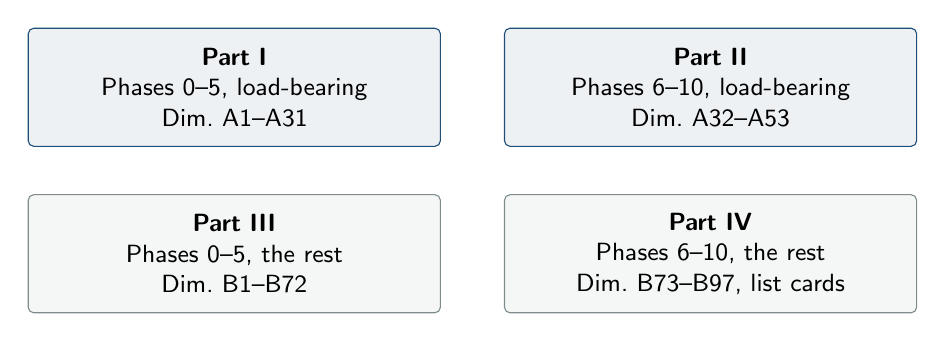
\begin{tikzpicture}[font=\small\sffamily]
\node[draw=cA,fill=cA!8,rounded corners=2pt,text width=5.0cm,align=center,minimum height=15mm] (a) {\textbf{Part I}\\ Phases 0--5, load-bearing\\ Dim.~A1--A31};
\node[draw=cA,fill=cA!8,rounded corners=2pt,text width=5.0cm,align=center,minimum height=15mm,right=8mm of a] (b) {\textbf{Part II}\\ Phases 6--10, load-bearing\\ Dim.~A32--A53};
\node[draw=cG,fill=cG!8,rounded corners=2pt,text width=5.0cm,align=center,minimum height=15mm,below=6mm of a] (c) {\textbf{Part III}\\ Phases 0--5, the rest\\ Dim.~B1--B72};
\node[draw=cG,fill=cG!8,rounded corners=2pt,text width=5.0cm,align=center,minimum height=15mm,right=8mm of c] (d) {\textbf{Part IV}\\ Phases 6--10, the rest\\ Dim.~B73--B97, list cards};
\end{tikzpicture}
\vfill
{\small Every card carries its ledger identifier, its trust label, and the page of the statement in the companion paper \emph{Exact Recovery of a Differential Operator from a Single Solution, complete edition, Phases~0--10}.\par}
\vspace{0.4cm}
{\small October 2026\par}
\end{titlepage}


% ---- begin c_front_all.tex
\chapter*{How to read this catalogue}
\addcontentsline{toc}{chapter}{How to read this catalogue}

This volume contains the proofs of the results stated in the paper \emph{Exact Recovery of a Linear Differential Operator from a Single Solution} (complete edition, Phases~0--10). It is a catalogue: every result has one card, and every card has the same shape.

\section*{The shape of a card}

\begin{dimcard}{A0}{ID-T0}{Name of the result}{\proved}{}
The full statement, with every hypothesis.
\end{dimcard}
\begin{proofidea}
One paragraph that says why the result is true, before any computation.
\end{proofidea}
\begin{proof}
\step{1}{First claim}
One claim per step, with its computation displayed on its own line.
\step{2}{Second claim}
\dots
\whyworks{one sentence that names the mechanism of the proof.}
\end{proof}
\uses{the results this proof relies on, by catalogue number.}

\section*{The four parts}

\textbf{Part~I} contains the 31 results of Phases~0--5 on which everything else rests (Dim.~A1--A31). They were selected from the project's dependency graph: a result is in Part~I if many other results depend on it, or if it is a headline theorem of the paper. Their proofs are given in full, step by step.

\textbf{Part~II} contains the load-bearing results of Phases~6--10 (Dim.~A32--A53): systems and gauge, variable coefficients, convergence and noise, the analytic encoder, the universal dictionary, and the Phase~10 corrections to results of Phases~0--5. They were selected by the same criterion: use in the extended algorithm (the section ``The extended algorithm'' of the paper of the paper), dependence in the ledger, and headline status.

\textbf{Part~III} contains all the other results of Phases~0--5, grouped by phase and ordered by identifier (Dim.~B1--B72). Short and medium proofs are given in full. Proofs that take many pages in the research files (the Burgers asymptotics, the scattering identification, the Hirota computations) are given as a condensed card, with every step and key formula and a pointer to the research file.

\textbf{Part~IV} contains the other results of Phases~6--10 (Dim.~B73--B155 and list cards). Eighty-three results have a card with a proof (Dim.~B73--B155); the others are \emph{list cards}: the statement, its trust label and the research file that holds the proof. All proofs of Part~II and Part~IV were rewritten from the research packages for this volume and were not re-audited; the trust label refers to the result as recorded in the ledger. This is a deliberate limit of this edition: for Phases~6--10 the research packages are about $150{,}000$ words, and only the proofs that the extended algorithm or a corrected statement depends on were rewritten here.

\textbf{Which edition to read.} The companion volumes for Phases~0--5 alone are \emph{paper\_fasi05} and \emph{dimostrazioni\_fasi05}. In case of a difference, this volume prevails: Phase~10 refuted or corrected several statements of Phases~0--5 (Chapter~\ref{ch:cIII6}).

\section*{Trust labels}

\begin{center}\small
\begin{tabular}{@{}L{4.4cm}L{10.0cm}@{}}
\toprule
Label & Meaning\\\midrule
\proved & complete proof, passed an independent review\\
\modulo{X} & complete except for a cited published theorem X, whose source was checked\\
\pw & complete proof, not independently reviewed\\
\cf & a published theorem, used as a black box\\
\condl & depends on a lemma that is not proved\\
\vex & checked on examples only\\
\falsest & a counterexample is proved (the card proves the counterexample)\\
\openq & unsolved\\\bottomrule
\end{tabular}
\end{center}

The reviewers were independent AI agents, not human referees. Identifiers such as C3-T1 are those of the project ledger \texttt{claims/LEDGER.md}; the research file that holds each original proof is named in the index at the end.

\section*{The backbone of Part~I (Phases~0--5)}

\begin{center}
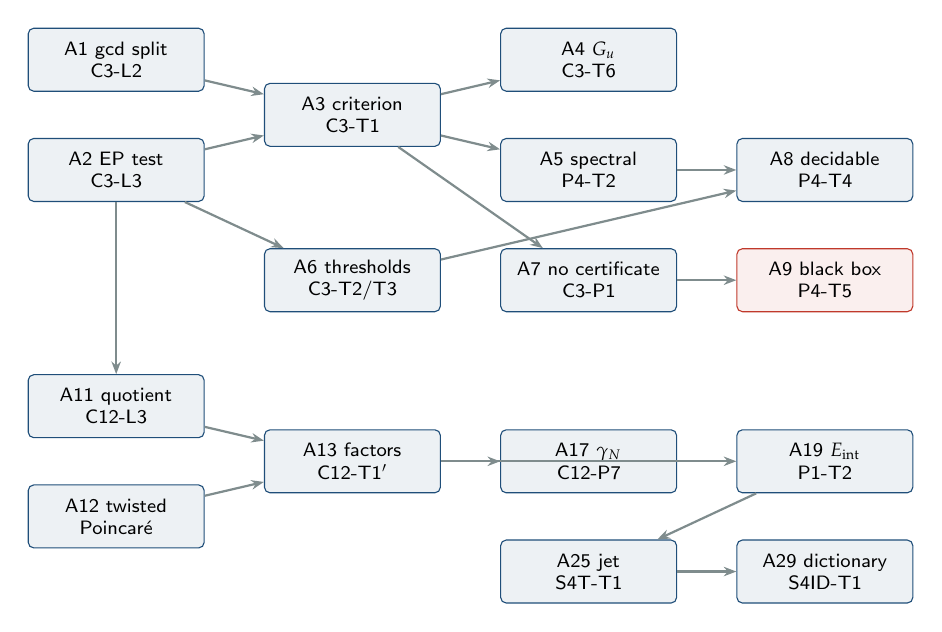
\begin{tikzpicture}[x=1cm,y=1cm,
  n/.style={draw=cA,fill=cA!8,rounded corners=2pt,font=\scriptsize\sffamily,align=center,minimum height=8mm,text width=2.0cm},
  m/.style={draw=cB,fill=cB!8,rounded corners=2pt,font=\scriptsize\sffamily,align=center,minimum height=8mm,text width=2.0cm},
  a/.style={-{Stealth[length=1.6mm]},cG,thick}]
\node[n] (L2) at (0,0) {A1 gcd split\\C3-L2};
\node[n] (L3) at (0,-1.4) {A2 EP test\\C3-L3};
\node[n] (T1) at (3,-0.7) {A3 criterion\\C3-T1};
\node[n] (T6) at (6,0) {A4 $G_u$\\C3-T6};
\node[n] (P4) at (6,-1.4) {A5 spectral\\P4-T2};
\node[n] (T3) at (3,-2.8) {A6 thresholds\\C3-T2/T3};
\node[n] (P1) at (6,-2.8) {A7 no certificate\\C3-P1};
\node[n] (T4) at (9,-1.4) {A8 decidable\\P4-T4};
\node[m] (T5) at (9,-2.8) {A9 black box\\P4-T5};
\node[n] (CL3) at (0,-4.4) {A11 quotient\\C12-L3};
\node[n] (L1p) at (0,-5.8) {A12 twisted\\Poincar\'e};
\node[n] (T1p) at (3,-5.1) {A13 factors\\C12-T1$'$};
\node[n] (P7) at (6,-5.1) {A17 $\gamma_N$\\C12-P7};
\node[n] (P1T2) at (9,-5.1) {A19 $\Eint$\\P1-T2};
\node[n] (S4) at (9,-6.5) {A29 dictionary\\S4ID-T1};
\node[n] (J) at (6,-6.5) {A25 jet\\S4T-T1};
\draw[a] (L2)--(T1); \draw[a] (L3)--(T1); \draw[a] (T1)--(T6); \draw[a] (T1)--(P4);
\draw[a] (L3)--(T3); \draw[a] (T3)--(T4); \draw[a] (P4)--(T4); \draw[a] (T1)--(P1); \draw[a] (P1)--(T5);
\draw[a] (CL3)--(T1p); \draw[a] (L1p)--(T1p); \draw[a] (T1p)--(P7); \draw[a] (T1p)--(P1T2);
\draw[a] (P1T2)--(J); \draw[a] (L3)--(CL3);
\draw[a] (J)--(S4);
\end{tikzpicture}
\end{center}
{\small The arrows mean ``is used in the proof of''. Blue: positive results; red: a negative (impossibility) result. The arrows come from the \texttt{depends\_on} edges of the project graph.}

% ---- end c_front_all.tex

\tableofcontents
\clearpage
\pagenumbering{arabic}

\part{Phases 0--5: the load-bearing proofs}

% ---- begin c_I1.tex
\chapter{Algebra and identification}\label{ch:cI1}
\chapterbrief
{$\Omega\subset\R^2$ open and connected; the ring $\ring=\C[\tau,\xi]$ acting on distributions by $\tau\mapsto\partial_t$, $\xi\mapsto\partial_x$. Classical facts used without proof: unique factorisation in $\ring$ (Gauss), the Nullstellensatz, the Chinese remainder theorem, and the fact that distributions agreeing near every point agree.}
{every identification argument reduces a question about solutions to a question about ideals and exponential-polynomials. This chapter proves those reductions in full, then the identification theorems built on them.}
{Dim.~A1--A9. They prove Chapters~3--5 of the paper: the gcd splitting, the EP test, the identification criterion, the intrinsic operator, the spectral form, the finite-data thresholds, and the decidability results.}

\begin{notebox}{Notation for the whole chapter}
$\Var(I)\subset\C^2$ is the common zero set of an ideal $I$. For a point $z=(\tau_z,\xi_z)\in\C^2$,
\[
\mathfrak m_z=(\tau-\tau_z,\ \xi-\xi_z)
\]
is its maximal ideal, and $e^{\langle z,\cdot\rangle}$ denotes $e^{\tau_zt+\xi_zx}$. $\Ann(w)=\{Q\in\ring:\ Q(\partial)w=0\}$. $\EP(\Omega)$ is the set of restrictions to $\Omega$ of finite sums $\sum_kq_k\,e^{\langle z_k,\cdot\rangle}$ with polynomials $q_k$.
\end{notebox}

%=====================================================================
\section{The algebraic toolkit}

\begin{dimcard}{A1}{C3-L2}{Splitting off the gcd}{\proved}{lem:gcd}
Let $0\ne I\subseteq\ring$ be an ideal and $G=\Gcd(I)$. Then:
\begin{enumerate}[label=(\roman*)]
\item $I=G\cdot J$ for an ideal $J$ with $\Gcd(J)=1$;
\item $\Var(J)$ is finite;
\item $(\sqrt J)^N\subseteq J$ for some $N$, and $J=\ring$ if $\Var(J)=\emptyset$.
\end{enumerate}
Two facts are proved on the way:
\begin{itemize}
\item \textbf{(V)} two nonzero coprime polynomials have finitely many common zeros;
\item \textbf{(F)} an irreducible polynomial has infinitely many zeros; hence if $\Var(\Ann w)$ is finite, some $h\in\Ann(w)$ is not divisible by a given irreducible $P_i$.
\end{itemize}
\end{dimcard}

\begin{proofidea}
Over the field $\C(\xi)$ two coprime polynomials have a B\'ezout identity; clearing denominators gives a polynomial in $\xi$ alone that vanishes at every common zero, and likewise in $\tau$. After dividing an ideal by its gcd, a generic combination of its elements is coprime to any fixed element, and (V) applies.
\end{proofidea}

\begin{proof}
\step{1}{Fact (V): coprime polynomials meet in finitely many points}
Let $f,g\ne0$ be coprime and $K=\C(\xi)$. A common factor of positive $\tau$-degree in $K[\tau]$ would give, by the Gauss lemma, a common factor in $\C[\xi][\tau]$; so $f,g$ are coprime in the principal ideal domain $K[\tau]$. Hence there are $a,b\in K[\tau]$ with
\[
af+bg=1 .
\]
Multiplying by a common denominator,
\[
a'f+b'g=r(\xi),\qquad a',b'\in\ring,\quad r\in\C[\xi]\setminus\{0\}.
\]
At a common zero $(\tau_0,\xi_0)$ the left side vanishes, so $r(\xi_0)=0$: finitely many $\xi_0$. Exchanging $\tau$ and $\xi$ gives $s(\tau)\ne0$ with $s(\tau_0)=0$. Therefore
\[
\Var(f,g)\subseteq\{r=0\}\times\{s=0\},
\]
a finite set.

\step{2}{Fact (F): an irreducible polynomial has infinitely many zeros}
If $\deg_\tau P_i\ge1$, then for all $\xi_0$ outside the finitely many zeros of the leading coefficient, $P_i(\cdot,\xi_0)$ has a root $\tau_0$. This gives infinitely many points. If $\deg_\tau P_i=0$, then $P_i$ is an irreducible polynomial in $\xi$, so $P_i=\alpha(\xi-\xi_0)$ and $\Var(P_i)=\C\times\{\xi_0\}$.

For the consequence: if every $h\in\Ann(w)$ were divisible by $P_i$, then $\Var(P_i)\subseteq\Var(\Ann w)$, an infinite set inside a finite one.

\step{3}{(i) Dividing by the gcd}
Put $J=\{f/G:\ f\in I\}$. It is closed under sums and under multiplication by $\ring$, so it is an ideal, and $I=G\cdot J$. If a prime $\pi$ divided every element of $J$, then $G\pi$ would divide every element of $I$, against the definition of $G$. So $\Gcd(J)=1$.

\step{4}{(ii) A generic combination is coprime to a fixed element}
If $J=\ring$ there is nothing to prove. Otherwise pick $0\ne f\in J$ with distinct prime factors $\pi_1,\dots,\pi_s$. By Step~3, for each $a$ there is $g_a\in J$ with $\pi_a\nmid g_a$. For $c\in\C^s$ put
\[
g_c=\sum_{b=1}^sc_b\,g_b\in J .
\]
For each $a$ the set $H_a=\{c:\ \pi_a\mid g_c\}$ is a linear subspace, and it is proper because the $a$-th unit vector is not in it. A finite union of proper subspaces does not cover $\C^s$, so some $c$ lies in no $H_a$. Then $f$ and $g_c$ are coprime, and by Step~1
\[
\Var(J)\subseteq\Var(f,g_c)\quad\text{is finite.}
\]

\step{5}{(iii) Nullstellensatz}
The polynomials vanishing on $\Var(J)$ form $\sqrt J$, which is finitely generated, so a power of it lies in $J$. If $\Var(J)=\emptyset$, then $\sqrt J=\ring$ and $1\in J$.

\whyworks{dividing by the gcd leaves an ideal with no common curve, and two curves without common component meet in finitely many points.}
\end{proof}
\uses{Gauss lemma, Nullstellensatz.}

%---------------------------------------------------------------------
\begin{dimcard}{A2}{C3-L3}{Exponential-polynomials are the finite-dimensional functions}{\proved}{lem:ep}
For $w\in\mathcal D'(\Omega)$, $\Omega$ connected, the following are equivalent:
\[
w\in\EP(\Omega)\iff\dimc_\C\ring w<\infty\iff\Var(\Ann w)\ \text{is finite.}
\]
Moreover, with distinct $z_k$:
\begin{enumerate}[label=(\alph*)]
\item $Q(\partial)\big(q\,e^{\langle z,\cdot\rangle}\big)=\big(Q(z+\partial)q\big)\,e^{\langle z,\cdot\rangle}$ for every polynomial $q$;
\item if $\sum_kq_k\,e^{\langle z_k,\cdot\rangle}=0$ on a nonempty open set, every $q_k=0$;
\item if $w=\sum_kq_k\,e^{\langle z_k,\cdot\rangle}$ with $q_k\ne0$, then $\Var(\Ann w)=\{z_k\}$.
\end{enumerate}
\end{dimcard}

\begin{proofidea}
Exponentials are independent, so an exponential-polynomial lives on finitely many points. Conversely, a finite-dimensional derivative-stable space gives two one-variable ODEs, $p(\partial_t)w=0$ and $q(\partial_x)w=0$. On a rectangle they force $w$ to be an exponential-polynomial, and connectedness glues the rectangles together.
\end{proofidea}

\begin{proof}
\step{1}{(a) Derivatives of an exponential times a polynomial}
For one derivative,
\[
\partial_t\big(q\,e^{\langle z,\cdot\rangle}\big)=\big(\partial_tq+\tau_zq\big)\,e^{\langle z,\cdot\rangle},
\]
and the same with $\partial_x$ and $\xi_z$. Iterating and using linearity gives (a).

\step{2}{(b) Exponentials are linearly independent}
The sum is real-analytic on $\R^2$ and vanishes on an open set, so it vanishes everywhere. Suppose some $q_k\ne0$, and let $K'$ be the set of such $k$. Choose $v\in\R^2$ with $\langle z_k-z_l,v\rangle\ne0$ for $k\ne l$, and $y_0$ with $\prod_{K'}q_k(y_0)\ne0$. Restricting to the line $y_0+sv$ gives
\[
f(s)=\sum_{k\in K'}r_k(s)\,e^{\mu_ks}\equiv0,\qquad \mu_k=\langle z_k,v\rangle\ \text{distinct},\quad r_k(0)\ne0 .
\]
We remove one term at a time. Multiply by $e^{-\mu_1s}$ and differentiate $\deg r_1+1$ times. The first term disappears. Each other term becomes
\[
\Big(\big(D+\mu_k-\mu_1\big)^{\deg r_1+1}r_k\Big)\,e^{(\mu_k-\mu_1)s},
\]
and since $\mu_k\ne\mu_1$ the operator $(D+c)^N$ with $c\ne0$ preserves the degree, so the new coefficient is nonzero. Induction ends with $r(s)e^{\mu s}\equiv0$, $r\ne0$: impossible.

\step{3}{(c) The zero set of the annihilator is the set of exponents}
By (a), the derivatives of $q\,e^{\langle z,\cdot\rangle}$ stay in $\C[t,x]_{\le\deg q}\cdot e^{\langle z,\cdot\rangle}$, which is finite-dimensional. If $|\beta|>\deg q$, the product $(\tau-\tau_z)^{\beta_1}(\xi-\xi_z)^{\beta_2}$ acts on $q$ as $\partial^\beta$ and kills it. So
\[
\prod_k\mathfrak m_{z_k}^{\deg q_k+1}\subseteq\Ann(w),\qquad \Var(\Ann w)\subseteq\{z_k\}.
\]
Conversely, if $Q\in\Ann(w)$ then $Q(z_k+\partial)q_k=0$ by (a) and (b). The top-degree part of $Q(z_k+\partial)q_k$ is $Q(z_k)$ times the top-degree part of $q_k$, so $Q(z_k)=0$.

\step{4}{Finite zero set implies finite dimension}
If $\Var(\Ann w)=\emptyset$ then $\Ann w=\ring$ and $w=0$. Otherwise, by A1(iii),
\[
\Ann(w)\supseteq\mathfrak I(\Var)^N,
\]
where $\mathfrak I(\Var)$ is the ideal of the finite set $\Var=\Var(\Ann w)$. By the Chinese remainder theorem
\[
\ring/\mathfrak I(\Var)^N\cong\bigoplus_{z\in\Var}\ring/\mathfrak m_z^N,
\]
which is finite-dimensional. Hence $\ring w\cong\ring/\Ann(w)$ is finite-dimensional too.

\step{5}{Finite dimension gives two ODEs}
Let $W=\ring w$, stable under $\partial_t$ and $\partial_x$. Let $p$ and $q$ be the minimal polynomials of $\partial_t|_W$ and $\partial_x|_W$. Then
\[
p(\partial_t)\,w=0,\qquad q(\partial_x)\,w=0 .
\]

\step{6}{On a rectangle the ODE in $t$ separates the variables}
Let $Q_0=I'\times J'\subset\Omega$ be an open rectangle. We claim that every $v\in\mathcal D'(Q_0)$ with $p(\partial_t)v=0$ has the form
\[
v=\sum_{j,l}c_{jl}\otimes t^le^{\lambda_jt},\qquad c_{jl}\in\mathcal D'(J'),
\]
with $\lambda_j$ the roots of $p$. Induction on $\deg p$. Write $p=(\tau-\lambda)\tilde p$. By induction $(\partial_t-\lambda)v=\sum\tilde c_{jl}\otimes t^le^{\lambda_jt}$. Each summand has a particular solution $\tilde c\otimes g(t)$:
\[
g=r(t)\,e^{\lambda_jt}\ (\deg r=l)\ \text{ if }\lambda_j\ne\lambda,\qquad g=\frac{t^{l+1}e^{\lambda t}}{l+1}\ \text{ if }\lambda_j=\lambda .
\]
With $v_p$ their sum, $\partial_t\big(e^{-\lambda t}(v-v_p)\big)=0$.

A distribution $V$ on $J'\times I'$ with $\partial_tV=0$ is $c\otimes1$. Indeed, fix $\chi\in C_c^\infty(I')$ with $\int\chi=1$. For a test function $\varphi$ put $\Phi(x)=\int\varphi(x,t)\dd t$ and
\[
\psi(x,t)=\int_{-\infty}^t\big(\varphi(x,s)-\chi(s)\Phi(x)\big)\dd s .
\]
Since $I'$ is an interval, $\psi$ has compact support, and $\varphi=\chi\otimes\Phi+\partial_t\psi$. Hence $V(\varphi)=V(\chi\otimes\Phi)$, which depends only on $\Phi$. So $v=v_p+c\otimes e^{\lambda t}$, completing the induction.

\step{7}{The ODE in $x$ makes the coefficients exponential-polynomials}
Applying $q(\partial_x)$:
\[
\sum_{j,l}q(\partial_x)c_{jl}\otimes t^le^{\lambda_jt}=0 .
\]
The functions $g_a=t^le^{\lambda_jt}$ are independent on $I'$, so there are test functions $\psi_b$ with $\int g_a\psi_b=\delta_{ab}$. Testing against $\varphi(x)\psi_b(t)$ gives $q(\partial_x)c_{jl}=0$. The one-variable case of Step~6 gives $c_{jl}\in\EP(J')$. So $w$ restricted to $Q_0$ is the restriction of an exponential-polynomial $E_{Q_0}$ on $\R^2$.

\step{8}{Connectedness glues the rectangles}
Fix $Q_0$ and $E=E_{Q_0}$. Let $A=\{y\in\Omega:\ w=E\ \text{near }y\}$. It is open and nonempty. It is closed in $\Omega$: if $y\in\bar A$, take a rectangle $Q_y\ni y$. On the open set $Q_y\cap A$ we have $E_{Q_y}=w=E$, so by Step~2 the exponential-polynomial $E_{Q_y}-E$ vanishes identically, and $w=E$ near $y$. By connectedness $A=\Omega$, so $w=E|_\Omega\in\EP(\Omega)$.

\whyworks{finite dimension turns differentiation into two commuting matrices; their eigenvalues are the exponents, and rectangles plus connectedness globalise the local form.}
\end{proof}
\uses{A1.}

\begin{caution}[title={Why rectangles in Step~6}]
On a U-shaped region, $v=\phi(x)\mathbf 1_{t>2}$ (with $\phi=0$ for $x<1$, $\phi=1$ for $x>2$) is smooth and satisfies $\partial_tv=0$, but it is not of the form $c(x)\otimes1$. So the local form is proved on rectangles and glued in Step~8. This $v$ is not a counterexample to A2: its derivative space is infinite-dimensional.
\end{caution}

%=====================================================================
\section{The identification theorems}

\begin{dimcard}{A3}{C3-T1}{Identification criterion}{\proved}{thm:ident}
Let $\Omega$ be connected, $u\in\mathcal D'(\Omega)$, $P(\partial)u=0$ with $P=c\prod_iP_i^{e_i}$ nonconstant, and
\[
w_i=\Big(\frac{P}{P_i}\Big)(\partial)u,\qquad w_i'=\Big(\frac{P}{P_i^{e_i}}\Big)(\partial)u .
\]
\begin{enumerate}[label=(\alph*)]
\item $\Ann(u)=(P)\iff w_i\notin\EP(\Omega)$ for every $i$.
\item $\Var(\Ann u)=\Var(P)\iff w_i'\notin\EP(\Omega)$ for every $i$.
\item If $P$ is squarefree, the two conditions coincide.
\item If $P$ is monic in $\tau$ of degree $m$: $\Ann(u)=(P)$ iff the only $(b_0,\dots,b_{m-1})\in\C[\xi]^m$ with $\sum_jb_j(\partial_x)\partial_t^ju=0$ is zero.
\item In general $\Ann(u)=G\cdot J$ with $G\mid P$, $\Var(J)$ finite, and $G\sim P\iff\Ann(u)=(P)$.
\end{enumerate}
\end{dimcard}

\begin{proofidea}
Write $\Ann(u)=G\cdot J$. If $G$ misses a copy of some $P_i$, then $w_i$ is killed by a power of the ideal of the finite set $\Var(J)$, so it is an exponential-polynomial. Conversely, an exponential-polynomial $w_i$ is killed by some $h$ coprime to $P_i$, and $h\cdot P/P_i$ is an annihilator of $u$ that $P$ does not divide.
\end{proofidea}

\begin{proof}
Let $I=\Ann(u)$. It contains $P$. By A1, $I=G\cdot J$ with $G=\Gcd I$ dividing $P$, so
\[
G=c'\prod_iP_i^{f_i},\qquad 0\le f_i\le e_i .
\]

\step{1}{(e) $G\sim P$ exactly when $I=(P)$}
If $G\sim P$, then $I=PJ\subseteq(P)\subseteq I$. If $I=(P)$, then $P$ divides every element of $I$ and is itself in $I$, so it is the gcd.

\step{2}{(a), first direction: if $I\ne(P)$, some $w_i$ is an exponential-polynomial}
If $I\ne(P)$, then $G\not\sim P$, so some $f_i<e_i$, and $P/P_i=G\,H$ for some $H\in\ring$. By A1(iii), $J\supseteq\mathfrak n^N$ with $\mathfrak n$ the ideal of $\Var(J)$. For $h\in\mathfrak n^N$:
\[
h\cdot\frac{P}{P_i}=G\,(Hh)\in G\,J=I,
\qquad\text{so}\qquad h(\partial)\,w_i=0 .
\]
Hence $\Ann(w_i)\supseteq\mathfrak n^N$, its zero set lies in the finite $\Var(J)$, and $w_i\in\EP$ by A2.

\step{3}{(a), second direction: an exponential-polynomial $w_i$ gives a new annihilator}
Suppose $w_i\in\EP$. Then $\Var(\Ann w_i)$ is finite, so by A1(F) some $h\in\Ann(w_i)$ has $P_i\nmid h$. Put
\[
Q=h\cdot\frac{P}{P_i}.
\]
Then $Q(\partial)u=h(\partial)w_i=0$, so $Q\in I$. If $Q=PA$, cancelling $P/P_i$ in the domain $\ring$ gives $h=P_iA$, a contradiction. So $Q\in I\setminus(P)$.

\step{4}{(b) The variety sees only whether each $f_i\ge1$}
We have $\Var(I)=\Var(G)\cup\Var(J)$, with $\Var(J)$ finite. If $f_i\ge1$, then $\Var(P_i)\subseteq\Var(G)\subseteq\Var(I)$. If $f_i=0$, then $\Var(P_i)\cap\Var(I)$ lies in the finite set
\[
\bigcup_{f_j\ge1}\big(\Var(P_i)\cap\Var(P_j)\big)\ \cup\ \Var(J),
\]
while $\Var(P_i)$ is infinite, so $\Var(P_i)\not\subseteq\Var(I)$. Hence $\Var(I)=\Var(P)$ iff all $f_i\ge1$. Finally, $f_i=0$ iff $w_i'\in\EP$: one direction is Step~2 with $P/P_i^{e_i}$ in place of $P/P_i$; for the other, an $h\in\Ann(w_i')$ with $P_i\nmid h$ gives $G\mid h\,P/P_i^{e_i}$, and $P_i$ divides neither factor, so $f_i=0$.

\step{5}{(c) and (d)}
For $e_i=1$, $w_i=w_i'$, which is (c). For (d), divide by the monic $P$ in $\C[\xi][\tau]$:
\[
Q=AP+\sum_{j<m}b_j(\xi)\,\tau^j\quad\text{uniquely}.
\]
Since $A(\partial)P(\partial)u=0$, $Q\in I$ iff $\sum_jb_j(\partial_x)\partial_t^ju=0$, and $Q\in(P)$ iff all $b_j=0$.

\whyworks{the gcd of the annihilator records the infinite part of $u$; any factor it misses leaves behind a function killed by a zero-dimensional ideal, that is, an exponential-polynomial.}
\end{proof}
\uses{A1, A2.}

\begin{example}{The proof on a wave}
Let $P=\tau^2-\xi^2$ and $u=e^{x-t}+e^{-(x+t)^2}$. For the factor $P_i=\tau+\xi$:
\[
w_i=(\partial_t-\partial_x)u=-2e^{x-t}\in\EP .
\]
Step~3 takes $h=\xi-1$, which kills $e^{x-t}$ and is not a multiple of $\tau+\xi$, and produces
\[
Q=(\xi-1)(\tau-\xi)\in\Ann(u)\setminus(P).
\]
\end{example}

%---------------------------------------------------------------------
\begin{dimcard}{A4}{C3-T6}{The intrinsic operator}{\proved}{thm:intrinsic}
Let $0\ne P\in\Ann(u)$, $P=c\prod_iP_i^{e_i}$, and
\[
S_i=\Big\{k\in\{0,\dots,e_i\}:\ \Big(\frac{P}{P_i^k}\Big)(\partial)u\in\EP\Big\}.
\]
Then $G_u=\Gcd\Ann(u)\sim\prod_iP_i^{f_i}$ with $f_i=e_i-\max S_i$. Moreover $\Ann(u)$ is principal iff $G_u(\partial)u=0$, and then $\Ann(u)=(G_u)$.
\end{dimcard}

\begin{proofidea}
The multiplicity $f_i$ of $P_i$ in $G_u$ is detected by stripping copies of $P_i$ from $P$ one at a time: as long as fewer than $e_i-f_i$ copies are removed the leftover is an exponential-polynomial, and as soon as more are removed it is not.
\end{proofidea}

\begin{proof}
\step{1}{The key equivalence}
By A1, $\Ann(u)=G_uJ_u$ with $G_u\mid P$. We show, for $1\le k\le e_i$,
\[
f_i\le e_i-k\iff\Big(\frac{P}{P_i^k}\Big)(\partial)u\in\EP .
\]
($\Rightarrow$) Then $G_u\mid P/P_i^k$; write $P/P_i^k=G_uH$. As in A3, Step~2, $h\cdot P/P_i^k\in\Ann(u)$ for every $h$ in a power of the ideal of $\Var(J_u)$, so the function is an exponential-polynomial.

($\Leftarrow$) If it is an exponential-polynomial, pick $h$ in its annihilator with $P_i\nmid h$ (A1(F)). Then $G_u$ divides $h\cdot P/P_i^k$. Comparing multiplicities of $P_i$ gives $f_i\le e_i-k$.

\step{2}{Reading off $f_i$}
The equivalence holds trivially for $k=0$. So $S_i=\{0,1,\dots,e_i-f_i\}$, and $\max S_i=e_i-f_i$. (The set is an interval because $\EP$ is stable under derivatives:
\[
\Big(\frac{P}{P_i^{k-1}}\Big)(\partial)u=P_i(\partial)\Big[\Big(\frac{P}{P_i^k}\Big)(\partial)u\Big].)
\]

\step{3}{Principality}
If $G_u(\partial)u=0$, then $(G_u)\subseteq\Ann(u)=G_uJ_u\subseteq(G_u)$. Conversely, if $\Ann(u)=(Q)$, then $Q$ is the gcd: $Q\sim G_u$, and $G_u(\partial)u=0$.

\whyworks{each copy of $P_i$ that $u$ does not need leaves an exponential-polynomial behind; counting them gives the exponent.}
\end{proof}
\uses{A1, A2, A3.}

%---------------------------------------------------------------------
\begin{dimcard}{A5}{P4-T2}{Spectral theorem for the cyclic module}{\proved}{thm:spec}
Let $W=\ring u\cong\ring/I$ with $I=\Ann(u)=G\cdot J$ as in A1. A \emph{joint eigenvector} for $z\in\C^2$ is $w\in W$, $w\ne0$, with $\mathfrak m_z(\partial)w=0$; $\sigma_p(u)$ is the set of $z$ having one.
\begin{enumerate}[label=(\roman*)]
\item Every joint eigenvector for $z$ is $c\,e^{\langle z,\cdot\rangle}$ with $c\ne0$, and $\sigma_p(u)=\Var(J)$.
\item $W\cap\EP(\Omega)=\ring\,G(\partial)u\cong\ring/J$, of finite dimension $\dimc\ring/J$.
\item $\Ann(u)$ is principal $\iff J=\ring\iff\sigma_p(u)=\emptyset\iff W\cap\EP=0$.
\item Hence, if $P(\partial)u=0$: $\Ann(u)=(P)\iff\sigma_p(u)=\emptyset$ and $G\sim P$.
\end{enumerate}
\end{dimcard}

\begin{proofidea}
Translate statements about the quotient ring $\ring/I$ (maximal ideals, socle) into statements about $W$. The only analytic input is the EP test A2.
\end{proofidea}

\begin{proof}
Two small facts are used.
\begin{itemize}
\item \textbf{(LG)} If $G\mid(\tau-\tau_z)Q$ and $G\mid(\xi-\xi_z)Q$, then $G\mid Q$: in a unique factorisation domain the gcd of the two products is $Q$.
\item \textbf{(LS)} If $M\ne0$ is a module with $\mathfrak m_z^NM=0$, some $v\ne0$ in $M$ has $\mathfrak m_zv=0$: take $y\ne0$ and $k$ maximal with $\mathfrak m_z^ky\ne0$.
\end{itemize}

\step{1}{Joint eigenvectors are single exponentials}
If $w=Q(\partial)u\ne0$ and $\mathfrak m_z^N(\partial)w=0$, then $\Var(\Ann w)\subseteq\{z\}$, so $w\in\EP$ and by A2 $w=q\,e^{\langle z,\cdot\rangle}$. The eigenvector condition gives $\partial_tq=\partial_xq=0$: $q$ is a constant.

\step{2}{$\sigma_p(u)\subseteq\Var(J)$}
Let $Q(\partial)u$ be a joint eigenvector at $z$. Then $(\tau-\tau_z)Q$ and $(\xi-\xi_z)Q$ lie in $I\subseteq(G)$, so $G\mid Q$ by (LG). Write $Q=GQ'$. Cancelling $G$:
\[
(\tau-\tau_z)Q'\in J,\qquad (\xi-\xi_z)Q'\in J,\qquad Q'\notin J .
\]
So $\mathfrak m_z\subseteq(J:Q')\ne\ring$. As $\mathfrak m_z$ is maximal, $(J:Q')=\mathfrak m_z\supseteq J$, and $z\in\Var(J)$.

\step{3}{$\Var(J)\subseteq\sigma_p(u)$}
By A1(iii), $J\supseteq\prod_{z'\in\Var(J)}\mathfrak m_{z'}^N$, and by the Chinese remainder theorem
\[
\ring/J\cong\prod_{z'\in\Var(J)}\ring/\big(J+\mathfrak m_{z'}^N\big).
\]
The factor at $z$ is nonzero and killed by $\mathfrak m_z^N$. By (LS) it contains $v\ne0$ with $\mathfrak m_zv=0$. Through the isomorphism of Step~4 this gives a joint eigenvector $(vG)(\partial)u\ne0$.

\step{4}{The exponential-polynomial part is $\ring G(\partial)u$}
Since $\ring$ is a domain,
\[
\Ann\big(G(\partial)u\big)=(I:G)=\{Q:\ QG\in GJ\}=J .
\]
$\Var(J)$ is finite, so $G(\partial)u\in\EP$ and $\ring G(\partial)u\subseteq\EP$. Conversely, let $w=Q(\partial)u\in\EP$. For each prime factor $P_i$ of $G$, with multiplicity $f_i$, A1(F) gives $h\in\Ann(w)$ with $P_i\nmid h$. Then $hQ\in I\subseteq(G)$, so $P_i^{f_i}\mid hQ$ and $P_i^{f_i}\mid Q$. Hence $G\mid Q$ and $w\in\ring G(\partial)u$. The map $Q\mapsto(QG)(\partial)u$ is onto with kernel $J$, so the space is $\cong\ring/J$.

\step{5}{(iii) and (iv)}
$J=\ring\iff\Var(J)=\emptyset$ (A1(iii)) $\iff\sigma_p(u)=\emptyset$ (Steps~2--3). Also $J=\ring\iff I=(G)$ is principal, and $W\cap\EP\cong\ring/J=0\iff J=\ring$. Finally $\Ann(u)=(P)$ iff $I$ is principal and $G\sim P$.

\whyworks{the finite part $J$ of the annihilator is exactly the module of exponentials inside $\ring u$; its points are the eigenvalues.}
\end{proof}
\uses{A1, A2.}

\begin{caution}[title={An empty spectrum alone is not enough}]
Take $u=e^{x^2}$ and $P=\tau^2$. For $Q=Q_0(\xi)+\tau Q_1$ one has $Q(\partial)u=Q_0(\partial_x)e^{x^2}$, which vanishes only if $Q_0=0$. So $\Ann(u)=(\tau)$ is principal and $\sigma_p(u)=\emptyset$, but $\Ann(u)\ne(\tau^2)$. The spectrum sees $J_u$, not $G_u$; condition (iv) needs both.
\end{caution}

%=====================================================================
\section{Finite data}

\begin{dimcard}{A6}{C3-T2}{B\'ezout threshold and jet threshold}{\proved}{thm:bezout}
\textbf{(C3-T2)} Let $u=\sum_{k=1}^Mc_k\,e^{\langle z_k,\cdot\rangle}$ with distinct $z_k\in\Var(P)$ and $c_k\ne0$, $P$ squarefree, $n\ge\deg P$. If
\[
\big|\{z_k\}\cap\Var(P_i)\big|>n\deg P_i\qquad\text{for every }i,
\]
then $\Ann(u)\cap\ring_{\le n}=P\cdot\ring_{\le n-\deg P}$. The threshold cannot be lowered uniformly.

\phantomsection\label{dim:C3-T3}\textbf{(C3-T3)} Let $0\ne u\in\EP(\Omega)$, $d=\dimc\ring u$, $p_0\in\Omega$.
\begin{enumerate}[label=(\roman*)]
\item $\Ann(u)\cap\ring_{\le n}=\{Q\in\ring_{\le n}:\ \partial^\beta(Q(\partial)u)(p_0)=0\ \forall|\beta|\le d-1\}$.
\item $\Ann(u)$ is generated in degree $\le d$, so the jet of order $2d-1$ determines it.
\item The order $2d-1$ is optimal in the worst case.
\end{enumerate}
\end{dimcard}

\begin{proofidea}
For modes: an annihilator vanishes at every exponent, and B\'ezout bounds how many exponents a curve that does not contain $\Var(P_i)$ can pass through. For jets: inside the $d$-dimensional space $\ring u$, the subspaces of elements vanishing to order $k$ at $p_0$ shrink strictly, so after $d-1$ steps they are zero.
\end{proofidea}

\begin{proof}
\step{1}{Annihilators of a sum of modes}
By A2(a)(b), $Q(\partial)u=\sum_kc_kQ(z_k)\,e^{\langle z_k,\cdot\rangle}$, which is zero iff $Q(z_k)=0$ for all $k$.

\step{2}{B\'ezout forces every $P_i$ to divide $Q$}
Let $Q\in\Ann(u)$ with $\deg Q\le n$. If $Q=0$ there is nothing to prove; a nonzero constant cannot kill $u\ne0$. Suppose $P_i\nmid Q$. Then $Q$ and $P_i$ are coprime, and B\'ezout's theorem (the homogenisations have no common component, since the line at infinity divides neither) gives
\[
\big|\Var(Q)\cap\Var(P_i)\big|\le\deg Q\cdot\deg P_i\le n\deg P_i .
\]
But by Step~1, $\{z_k\}\cap\Var(P_i)\subseteq\Var(Q)\cap\Var(P_i)$ has more points. So $P_i\mid Q$ for every $i$, and since the $P_i$ are distinct primes, $P\mid Q$.

\step{3}{The threshold is sharp}
Take $Z_n=\{(j^2,\pm j):\ j=1,\dots,n\}$, $2n$ points on $\tau=\xi^2$, and
\[
Q_n=\prod_{j=1}^n(\tau-j^2).
\]
It has degree $n$, vanishes on $Z_n$, and is not a multiple of $\tau-\xi^2$ because it does not involve $\xi$.

\step{4}{(i) Vanishing subspaces shrink strictly}
Let $W=\ring u$ and
\[
K_k=\{w\in W:\ \partial^\beta w(p_0)=0\ \text{for all }|\beta|\le k\}.
\]
If $K_k=K_{k+1}$, then $K_k$ is stable under derivatives (if $w\in K_{k+1}$ then $\partial w\in K_k$), so every $w\in K_k$ has all derivatives zero at $p_0$; being analytic on a connected set, $w=0$. So the dimensions drop strictly until they reach $0$. Since $\dim K_0=d-1$, we get $K_{d-1}=0$. For $Q\in\ring_{\le n}$, $Q(\partial)u\in W$ vanishes iff it lies in $K_{d-1}$. Any upper bound $d'\ge d$ works as well.

\step{5}{(ii) Generators of low degree}
$\ring/\Ann(u)\cong W$ has dimension $d$. In a graded monomial order, the standard monomials form a set of $d$ elements closed under division. A standard monomial $\tau^a\xi^b$ has $(a+1)(b+1)\ge a+b+1$ divisors, all standard, so $a+b+1\le d$. The minimal generators of the initial ideal therefore have degree at most $d$, and so do the elements of the reduced Gr\"obner basis, which generate $\Ann(u)$. Apply (i) with $n=d$: the jet of order $2d-1$ suffices.

\step{6}{(iii) Optimality}
Let $u=\sum_{j=1}^de^{jx}$, so $d=\dimc\ring u$, and $n=d$. Then $\Ann(u)\cap\C[\xi]_{\le d}=\C\cdot Q_0$ with $Q_0=\prod_j(\xi-j)$. Put $m_k=\partial_x^ku(p_0)$. With only $|\beta|\le d-2$ the test of (i) is the Hankel system
\[
\sum_{i=0}^dq_i\,m_{k+i}=0,\qquad k=0,\dots,d-2,
\]
which has $d-1$ equations in $d+1$ unknowns, so a kernel $N$ of dimension at least $2$. Take $Q_1\in N\setminus\C Q_0$ and $Q'=Q_0+sQ_1$ with $s$ small: it has degree $d$ and $d$ simple roots $\mu_j$. Choose $w_j$ with $\sum_jw_j\mu_j^k=m_k$ for $k<d$ (Vandermonde) and set
\[
u'=\sum_jw_j\,e^{\mu_j(x-x_0)}.
\]
The moment sequences of $u$ and $u'$ satisfy the same recursion given by $Q'$ and agree for $k\le d-1$, hence for $k\le2d-2$. So $u$ and $u'$ have the same jet of order $2d-2$, but $Q'\in\Ann(u')\setminus\Ann(u)$.

\whyworks{finitely many exponentials are finitely many points; B\'ezout counts how many points a curve must miss, and the strict drop of vanishing subspaces counts how many derivatives are needed.}
\end{proof}
\uses{A1, A2.}

%---------------------------------------------------------------------
\begin{dimcard}{A7}{C3-P1}{No finite certificate}{\proved{} (jets) / \cf{} (functionals)}{thm:nocert}
Let $\Omega$ be connected, $p_0\in\Omega$, $P$ nonconstant, $u$ smooth with $P(\partial)u=0$, $K\ge0$, and $E_P=\ker P\cap\EP(\Omega)$.
\begin{enumerate}[label=(\roman*)]
\item $\bigcap_{v\in E_P}\Ann(v)=(P)$.
\item There is $v\in E_P$ with the same jet of order $K$ at $p_0$ as $u$; in particular $\Ann(v)\supsetneq(P)$.
\end{enumerate}
On convex $\Omega$ the same holds for any finitely many continuous linear functionals (Malgrange); on a non-convex region it can fail.
\end{dimcard}

\begin{proofidea}
By duality, the possible jets of solutions are cut out by the multiples of $P$. Exponential-polynomial solutions already cut out the same space, because for every $Q$ that is not a multiple of $P$ one builds a solution $s^{e-1}e^{\langle z,\cdot\rangle}$ that $Q$ does not kill.
\end{proofidea}

\begin{proof}
Pair an operator $Q$ of degree at most $K$ with a jet by
\[
\langle Q,J_Kw\rangle=\big(Q(\partial)w\big)(p_0).
\]

\step{1}{Vanishing on all of $E_P$ means annihilating all of $E_P$}
If $(Q(\partial)v)(p_0)=0$ for every $v\in E_P$, then, since $E_P$ is stable under derivatives, all derivatives of the exponential-polynomial $Q(\partial)v$ vanish at $p_0$. It is entire with zero Taylor series, so it is $0$. Hence $Q\in\bigcap_{v\in E_P}\Ann(v)$.

\step{2}{(i) A non-multiple of $P$ misses some exponential solution}
Let $Q\ne0$ with $P\nmid Q$. Some $i$ has $f=v_{P_i}(Q)<e_i$; write $Q=P_i^fQ'$ with $P_i\nmid Q'$. The sets $\Var(P_i)\cap\Var(\nabla P_i)$ and $\Var(P_i)\cap\Var(Q')$ are finite (A1(V)), while $\Var(P_i)$ is infinite. Pick $z\in\Var(P_i)$ with
\[
\nabla P_i(z)\ne0,\qquad Q'(z)\ne0,
\]
and a coordinate $s\in\{t,x\}$ with $\partial_sP_i(z)\ne0$. On polynomials in $s$, $P_i(z+\partial)$ lowers the degree by exactly one and $Q'(z+\partial)$ preserves it. Let $v=s^{e_i-1}e^{\langle z,\cdot\rangle}$. Then $P(z+\partial)s^{e_i-1}=0$, so $v\in E_P$, while $Q(z+\partial)s^{e_i-1}$ has degree $e_i-1-f\ge0$ and is nonzero. So $Q\notin\Ann(v)$.

\step{3}{(ii) Every jet of a solution is a jet of an exponential solution}
By Steps~1--2, every $Q$ of degree $\le K$ orthogonal to the jets of $E_P$ is a multiple of $P$, hence orthogonal to the jet of $u$. In finite dimension this means
\[
J_K(u)\in J_K(E_P),
\]
so a suitable $v\in E_P$ exists. Finally $\Ann(v)\supsetneq(P)$: if $v=0$ it is $\ring$; otherwise $\Var(\Ann v)$ is finite while $\Var(P)$ is infinite.

\step{4}{General functionals and convexity}
For general continuous functionals the analogue on convex $\Omega$ is Malgrange's approximation theorem (Ann.\ Inst.\ Fourier 6, Chap.~I \S2 Thm~2) \cf. Without convexity it fails: on a U-shaped region take $P=\tau$, $u=\phi(x)\mathbf 1_{t>2}$, and
\[
\ell(w)=w(5/2,5/2)-w(1/2,5/2).
\]
Then $\ell(u)=1$ while $\ell(v)=0$ for every $v\in\ker\partial_t$ with $\Ann(v)\ne(\tau)$.

\whyworks{finite data see a finite-dimensional shadow of $\ker P$, and exponential solutions already fill every such shadow.}
\end{proof}
\uses{A1, A2.}

%---------------------------------------------------------------------
\begin{dimcard}{A8}{P4-T4}{Decidability with a bound}{\proved}{thm:decide}
In the model M2$^+$ (exact jets at $p_0$ in a computable field $K$, plus a zero-test oracle):
\begin{enumerate}[label=(\roman*)]
\item for every finite-dimensional $\mathcal L\subseteq\ring$ with a basis over $K$, $\Ann(u)\cap\mathcal L$ is computable;
\item ``$\Ann(u)\ne(P)$'' is semi-decidable;
\item if an integer $B\ge\dimc(\ring u\cap\EP)$ is given, then with $N=B+\deg P-1$,
\[
\Ann(u)=(P)\iff\Ann(u)\cap\ring_{\le N}=(P)\cap\ring_{\le N},
\]
which is decidable. The test ``$Q(\partial)u\in\EP$?'' is then decidable, and $G_u$ is computable.
\end{enumerate}
\end{dimcard}

\begin{proofidea}
Linear algebra on jets gives a decreasing chain of candidate spaces that stabilises at the true annihilators; the zero oracle confirms when it has stabilised. If identification fails, a witness of small degree exists, and the bound $B$ says how small.
\end{proofidea}

\begin{proof}
\step{1}{(i) A decreasing chain of linear spaces}
Let
\[
A_k=\{Q\in\mathcal L:\ \partial^\beta\big(Q(\partial)u\big)(p_0)=0\ \text{for all }|\beta|\le k\}.
\]
It is the kernel of a matrix with entries $\partial^{\beta+\alpha}u(p_0)\in K$, so it has a computable basis. The chain $A_0\supseteq A_1\supseteq\dots\supseteq\Ann(u)\cap\mathcal L$ stabilises, and its limit is $\Ann(u)\cap\mathcal L$, because $Q(\partial)u$ is analytic with zero Taylor series at $p_0$. Algorithm: for $k=0,1,\dots$ compute a basis of $A_k$ and ask the oracle about each element; stop when all answers are ``zero''. It stops only when $A_k\subseteq\Ann(u)$, so it is correct, and it stops at the stabilisation index.

\step{2}{(ii) Semi-decision}
For $n=\deg P,\deg P+1,\dots$ compute $\Ann(u)\cap\ring_{\le n}$ by (i) and compare its dimension with that of $P\cdot\ring_{\le n-\deg P}$. If $\Ann(u)\ne(P)$, a witness $Q$ exists and the loop stops at $n=\max(\deg Q,\deg P)$.

\step{3}{(iii) A witness of degree at most $N$}
Suppose $\Ann(u)\ne(P)$. By A3, some $w_i=(P/P_i)(\partial)u$ is an exponential-polynomial in $\ring u$, so
\[
d_i=\dimc\ring w_i\le B .
\]
By A6(ii), $\Ann(w_i)$ is generated in degree $\le d_i$, and not all generators are divisible by $P_i$ (A1(F)). Pick such a generator $h$, so $\deg h\le B$. Then
\[
Q=h\cdot\frac{P}{P_i}\in\Ann(u)\setminus(P),\qquad \deg Q\le B+\deg P-1=N .
\]
The comparison in degree $N$ is computable by (i).

\step{4}{The EP test from the bound}
Let $w=Q(\partial)u$; its oracles follow from those of $u$. If $w\in\EP$, then $\dimc\ring w\le B$, so the minimal polynomials of $\partial_t$ and $\partial_x$ on $\ring w$ have degree $\le B$: there are nonzero $a(\tau),b(\xi)$ of degree $\le B$ in $\Ann(w)$. Conversely, such $a,b$ give a finite zero set and $w\in\EP$ (A2). Both searches are computable by (i). With this test, A4 computes $G_u$.

\whyworks{a failure of identification is always witnessed in bounded degree, and the bound $B$ makes that degree explicit.}
\end{proof}
\uses{A1, A2, A3, A4, A6.}

%---------------------------------------------------------------------
\begin{dimcard}{A9}{P4-T5}{Black-box impossibility}{\proved}{thm:blackbox}
Let $P\in K[\tau,\xi]$ be nonconstant ($K$ the algebraic numbers), $\Omega$ connected, $p_0\in\Omega$ with coordinates in $K\cap\R$, and $u$ real-analytic with $P(\partial)u=0$, jets in $K$, and $\Ann(u)=(P)$ (such $u$ exists for every $P$, \led{P4-L7}). For every order $k_0$ and every finite set $\mathcal Q\subset K[\tau,\xi]$ there is an exponential-polynomial $v\in\ker P$ with
\begin{itemize}
\item the same jet of order $k_0$ at $p_0$ as $u$;
\item for every $Q\in\mathcal Q$: $Q(\partial)v=0\iff Q(\partial)u=0$;
\item $\Ann(v)\supsetneq(P)$.
\end{itemize}
Hence no algorithm in the model M2$^+$ decides ``$\Ann(\cdot)=(P)$'' correctly on all inputs.
\end{dimcard}

\begin{proofidea}
Run a correct algorithm on $u$: it halts after finitely many questions. An adversary builds $v$ among the exponential-polynomial solutions so that it gives the same answer to every one of those questions. First match the jet, then, for each $Q$ with $Q(\partial)u\ne0$, add a solution with zero jet that $Q$ does not kill, with generic coefficients.
\end{proofidea}

\begin{proof}
\step{1}{Witness points with algebraic coordinates}
Each $\Var(P_i)$ has infinitely many points with coordinates in $K$: roots of $P_i(\cdot,\xi_0)$ for $\xi_0\in K$, or $K\times\{\xi_0\}$ if $P_i$ does not involve $\tau$. For such $z$ with $\nabla P_i(z)\ne0$, pick a coordinate $s_z$ with $\partial_{s}P_i(z)\ne0$ and put
\[
g_{i,z,j}=s_z^{\,j}\,e^{\langle z,\cdot-p_0\rangle},\qquad j<e_i .
\]
As in A7, Step~2, $P(z+\partial)s_z^j=0$, so $g_{i,z,j}\in\ker P$.

\step{2}{Matching the jet}
Let $V_{k_0}$ be the span of the jets of order $k_0$ of all $g_{i,z,j}$. With the pairing of A7,
\[
V_{k_0}^\perp=(P)\cap\ring_{\le k_0};
\]
the inclusion ``$\subseteq$'' is A7, Step~2, with points chosen in $K^2$. Since $\langle PA,J_{k_0}u\rangle=0$, $J_{k_0}(u)\in V_{k_0}$. A linear system with coefficients in $K$ that is solvable over $\C$ is solvable over $K$, so some combination $v_1$ of the $g$'s has the jet of $u$.

\step{3}{A zero-jet solution for each test}
For $Q\in\mathcal Q\setminus(P)$ (so $Q(\partial)u\ne0$), pick $i$ with $f=v_{P_i}(Q)<e_i$, $Q=P_i^fQ'$, and more than $\dim\ring_{\le k_0}$ points $z\in\Var(P_i)\cap K^2$ with $\nabla P_i(z)\ne0$ and $Q'(z)\ne0$. The map
\[
c\ \mapsto\ J_{k_0}\Big(\sum_zc_z\,s_z^{e_i-1}e^{\langle z,\cdot-p_0\rangle}\Big)
\]
goes from a larger space to a smaller one, so it has a nonzero kernel vector $c$. Let $e_Q$ be the corresponding sum: its jet is $0$, while $Q(\partial)e_Q\ne0$ by A2(b).

\step{4}{A generic combination answers like $u$}
Let $v_\lambda=v_1+\sum_Q\lambda_Q\,e_Q$. It has the jet of $u$ for every $\lambda$. For each $Q$ with $Q(\partial)u\ne0$, the set $\{\lambda:\ Q(\partial)v_\lambda=0\}$ is a proper affine subspace. Finitely many proper subspaces do not cover the space, so some $\lambda$ avoids all of them. For $Q\in(P)$ both answers are ``zero''. So $v=v_\lambda$ answers every question as $u$ does, and $v\in\EP\cap\ker P$ gives $\Ann(v)\supsetneq(P)$.

\step{5}{Conclusion}
The run of the algorithm on $u$ depends only on the answers it receives. They coincide for $v$, so it outputs ``$\Ann=(P)$'' on $v$ as well, which is wrong.

\whyworks{a finite conversation with a black box can always be imitated by a finite sum of exponentials, and such sums never identify.}
\end{proof}
\uses{A2, A7.}

% ---- end c_I1.tex


% ---- begin c_I2.tex
\chapter{Decomposition and regularity}\label{ch:cI2}
\chapterbrief
{$P=c\prod_{j=1}^sQ_j$ with $Q_j=P_j^{m_j}$ pairwise coprime; $\Omega\subset\R^2$ open; $\mathcal A$ is $\mathcal D'(\Omega)$ or $C^\infty(\Omega)$; the toolkit of Chapter~\ref{ch:cI1}.}
{to prove that a solution splits into one piece per factor, with an ambiguity of exactly known size, that holes in $\Omega$ can break this, and exactly when the pieces keep the Sobolev regularity of $u$.}
{Dim.~A10--A18. They prove Chapters~6 and~7 of the paper.}

\begin{notebox}{Notation for the whole chapter}
For a module $M$ over $\ring$, $\mathrm{Sol}_{\mathcal A}(M)=\mathrm{Hom}_\ring(M,\mathcal A)$ is its solution space; for example $\mathrm{Sol}(\ring/(f))=\ker_{\mathcal A}f$. For $z=(p,q)\in\C^2$ we write $e_z=e^{pt+qx}$ and $D_t=\partial_t-p$, $D_x=\partial_x-q$. Note that $D_t(e_z\tilde w)=e_z\,\partial_t\tilde w$.
\end{notebox}

%=====================================================================
\section{Terms and factors}

\begin{dimcard}{A10}{R2-T3}{Terms do not give components}{\proved}{prop:terms}
Let $L=L_1+L_2\in\ring$.
\begin{enumerate}[label=(\alph*)]
\item In every $\ring$-module $\mathcal A$:
\[
\ker L\cap\big(\ker L_1+\ker L_2\big)\subseteq\mathrm{Sol}\big(\ring/(L,\ L_1L_2)\big)=\mathrm{Sol}\big(\ring/(L_1+L_2,\ L_1^2)\big).
\]
\item If $\mathcal A=C^\infty$ or $\mathcal D'$ of a convex $\Omega$ and $L_1,L_2$ are coprime, equality holds.
\item $\Var(L_1+L_2,\ L_1^2)=\Var(L_1)\cap\Var(L_2)$. For coprime $L_1,L_2$ the space is finite-dimensional, of dimension $2\sum_pI_p(L_1,L_2)$, and consists of exponential-polynomials with exponents at the common zeros.
\end{enumerate}
\end{dimcard}

\begin{proofidea}
A solution that splits by terms satisfies one extra equation, $L_1L_2u=0$, because the operators commute. Modulo $L$ that extra equation is $L_1^2$, and the common zeros of $L$ and $L_1^2$ are where both terms vanish.
\end{proofidea}

\begin{proof}
\step{1}{(a) The extra equation}
Let $u=u_1+u_2$ with $L_1u_1=0$ and $L_2u_2=0$. Since the operators commute,
\[
L_1L_2\,u=L_2(L_1u_1)+L_1(L_2u_2)=0 .
\]
Together with $Lu=0$ this gives $u\in\mathrm{Sol}(\ring/(L,L_1L_2))$. Modulo $L$, $L_2\equiv-L_1$, so $L_1L_2\equiv-L_1^2$ and the two ideals coincide.

\step{2}{(b) Equality from the decomposition theorem}
For coprime $L_1,L_2$ the finite module $\ring/(L_1,L_2)$ has no obstruction (A12), so the sequence of A13 is exact: every element of $\mathrm{Sol}(\ring/(L,L_1L_2))$ is killed by $L_1L_2$, hence by A13 splits as a sum of solutions of $L_1$ and of $L_2$.

\step{3}{(c) The variety}
On $\Var(L_1)$ we have $L_1+L_2=0\iff L_2=0$. Off $\Var(L_1)$, $L_1^2\ne0$. So
\[
\Var(L_1+L_2,\ L_1^2)=\Var(L_1)\cap\Var(L_2).
\]
For coprime terms this set is finite (A1(V)). The dimension follows from the additivity of intersection numbers, $I_p(F,GH)=I_p(F,G)+I_p(F,H)$, and $I_p(L_1+L_2,L_1)=I_p(L_2,L_1)$.

\whyworks{commuting terms turn a split by terms into an extra equation, which cuts the solution space down to the finitely many points where both terms vanish.}
\end{proof}
\uses{A1, A12, A13.}

\begin{example}{The heat equation as a sum of two terms}
Take $L_1=\partial_x^2$ and $L_2=-\partial_t$. The ideal is $(\xi^2-\tau,\ \xi^4)=(\tau^2,\ \xi^2-\tau)$, of dimension $4=2\cdot I_0(\xi^2,\tau)$. The solutions that split by terms are
\[
1,\qquad x,\qquad x^2+2t,\qquad x^3+6tx .
\]
The generic heat solution $e^{s^2t+sx}$ with $s\ne0$ has $L_1L_2u=-s^4u\ne0$, so it does not split.
\end{example}

%=====================================================================
\section{The factor decomposition}

\begin{dimcard}{A11}{C12-L3}{The finite quotient of two coprime factors}{\proved}{lem:C12L3}
Let $f,g,h\in\ring\setminus\{0\}$.
\begin{enumerate}[label=(\alph*)]
\item If $f,g$ are coprime, $(f,g)$ contains a nonzero $r(\xi)$ and a nonzero $s(\tau)$; hence $\dimc\ring/(f,g)<\infty$.
\item If $f$ is coprime to $g$ and to $h$, then
\[
\dimc\ring/(f,gh)=\dimc\ring/(f,g)+\dimc\ring/(f,h).
\]
\item $(f,g)=\ring\iff\Var(f)\cap\Var(g)=\emptyset$.
\end{enumerate}
\end{dimcard}

\begin{proofidea}
(a) is the B\'ezout identity of A1, Step~1. (b) is an exact sequence of finite-dimensional spaces. (c) uses that commuting operators on a nonzero finite-dimensional space have a common eigenvector.
\end{proofidea}

\begin{proof}
\step{1}{(a) A finite spanning set}
A1, Step~1 gives $r(\xi)\in(f,g)$ and symmetrically $s(\tau)\in(f,g)$, both nonzero. Then $\ring/(f,g)$ is spanned by the monomials
\[
\tau^a\xi^b,\qquad a<\deg s,\quad b<\deg r .
\]

\step{2}{(b) An exact sequence}
The sequence
\[
0\to\ring/(f,h)\xrightarrow{\ \cdot g\ }\ring/(f,gh)\to\ring/(f,g)\to0
\]
is well defined because $g\,(f,h)\subseteq(f,gh)$, and its middle is exact because the kernel of the projection is $(f,g)/(f,gh)$, the image of multiplication by $g$. Injectivity: if $ga=\alpha f+\beta gh$, then $g(a-\beta h)=\alpha f$; since $\Gcd(f,g)=1$, $f\mid a-\beta h$, so $a\in(f,h)$. Dimensions add.

\step{3}{(c) A common eigenvector gives a common zero}
($\Leftarrow$) If $f,g$ shared a nonconstant factor $\pi$, then $\emptyset\ne\Var(\pi)\subseteq\Var(f)\cap\Var(g)$ (A1(F)). So disjoint zero sets force coprimality, and (a) applies. If $(f,g)\ne\ring$, then $N=\ring/(f,g)$ is nonzero and finite-dimensional. The commuting operators $\tau,\xi$ on $N$ have a common eigenvector $v$, with eigenvalues $(p,q)$. Then $fv=gv=0$ gives $f(p,q)=g(p,q)=0$, a common zero.

($\Rightarrow$) If $(p,q)$ is a common zero, $(f,g)\subseteq\mathfrak m_{(p,q)}\ne\ring$.

\whyworks{coprime curves meet in finitely many points, and the quotient ring counts them with multiplicity.}
\end{proof}
\uses{A1.}

%---------------------------------------------------------------------
\begin{dimcard}{A12}{C12-L1'}{Twisted Poincar\'e lemma; no obstruction for finite modules}{\proved}{lem:twisted}
\phantomsection\label{dim:C12-L1p}%
Let $\Omega$ be open, connected, nonempty, with $H^1_{dR}(\Omega)=0$.
\begin{enumerate}[label=(\roman*)]
\item \textbf{(C12-L1$'$)} If $\varphi,\psi\in\mathcal A$ satisfy $D_x\varphi=D_t\psi$, there is $w\in\mathcal A$ with
\[
D_tw=\varphi,\qquad D_xw=\psi .
\]
Moreover $\{w\in\mathcal A:\ D_tw=D_xw=0\}=\C\,e_z$.
\item \textbf{(C12-L2$'$)} For every $\ring$-module $M$ with $n=\dimc M<\infty$:
\[
\mathrm{Ext}^1_\ring(M,\mathcal A)=0,\qquad \dimc\mathrm{Sol}_{\mathcal A}(M)=n,
\]
and every solution is the restriction of a unique exponential-polynomial solution on $\R^2$.
\end{enumerate}
\end{dimcard}

\begin{proofidea}
Multiplying by $e_z^{-1}$ turns the twisted derivatives into ordinary ones: (i) becomes ``a closed $1$-form is exact''. For distributions, solve locally on squares and glue; the gluing error is a smooth closed form, exact by hypothesis. (ii) follows from (i) for the simplest modules and by induction along a composition series.
\end{proofidea}

\begin{proof}
\step{1}{Removing the twist}
Put $\tilde\varphi=e_z^{-1}\varphi$ and $\tilde\psi=e_z^{-1}\psi$. The condition becomes
\[
\partial_x\tilde\varphi=\partial_t\tilde\psi,
\]
and we look for $\tilde w$ with $\partial_t\tilde w=\tilde\varphi$, $\partial_x\tilde w=\tilde\psi$; then $w=e_z\tilde w$.

\step{2}{Smooth case}
The $1$-form $\eta=\tilde\varphi\dd t+\tilde\psi\dd x$ is closed, hence exact because $H^1_{dR}(\Omega)=0$.

\step{3}{Distributions: local primitives glued by a partition of unity}
Cover $\Omega$ by open squares $U_j$ with closure in $\Omega$, and take a locally finite partition of unity $\chi_j\in C_c^\infty(U_j)$. On each square a primitive $w_j$ exists (integration in one variable, as in A2, Step~6). On an overlap $w_j-w_k$ has zero gradient, so it is a constant $c_{jk}$. Set $w=\sum_j\chi_jw_j$. On $U_k$,
\[
w-w_k=\sum_j\chi_j\,c_{jk}=:h_k\quad\text{is smooth.}
\]
So $a=\tilde\varphi-\partial_tw$ and $b=\tilde\psi-\partial_xw$ equal $-\partial_th_k$, $-\partial_xh_k$ locally. They form a smooth closed $1$-form, which is $d\theta$ for a smooth $\theta$ by hypothesis. Then $w+\theta$ is the required primitive.

\step{4}{The kernel}
If $\partial_t\tilde w=\partial_x\tilde w=0$, then $\tilde w$ is locally constant, hence constant on the connected $\Omega$.

\step{5}{(ii) The simplest module}
For $M=\ring/\mathfrak m_z$ use the Koszul resolution
\[
0\to\ring\xrightarrow{\ \beta\ }\ring^2\xrightarrow{\ \alpha\ }\ring\to\ring/\mathfrak m_z\to0 .
\]
Applying $\mathrm{Hom}(\cdot,\mathcal A)$, the solutions are $\ker(D_t,D_x)=\C e_z$ (Step~4) and $\mathrm{Ext}^1=\ker\beta^*/\mathrm{im}\,\alpha^*$, which is exactly the compatibility problem of (i): it vanishes.

\step{6}{(ii) Induction on the dimension}
A finite-dimensional $M$ has a composition series with factors $\ring/\mathfrak m_z$. The long exact sequence of $\mathrm{Ext}$ and induction on $n$ give $\mathrm{Ext}^1(M,\mathcal A)=0$ and $\dimc\mathrm{Sol}(M)=n$. On $\R^2$ the solutions are exponential-polynomials; restriction to $\Omega$ is injective (analytic functions vanishing on an open set vanish), and the dimensions agree.

\whyworks{on a region without holes, closed forms are exact, so finite systems of first-order equations are always solvable.}
\end{proof}
\uses{A2.}

%---------------------------------------------------------------------
\begin{dimcard}{A13}{C12-T1'}{Factor decomposition}{\proved}{thm:factor}
\phantomsection\label{dim:C12-T1p}%
Let $\Omega$ be open, connected, nonempty, with $H^1_{dR}(\Omega)=0$, $\mathcal A\in\{\mathcal D'(\Omega),C^\infty(\Omega)\}$, $P=c\prod_{j=1}^sQ_j$ with pairwise coprime $Q_j$.
\begin{enumerate}[label=(\roman*)]
\item $\ker_{\mathcal A}P=\ker_{\mathcal A}Q_1+\dots+\ker_{\mathcal A}Q_s$.
\item The kernel $\mathcal N$ of the sum map $\Sigma:\bigoplus_j\ker Q_j\to\ker P$ has dimension
\[
\delta(P)=\sum_{i<j}\dimc\ring/(Q_i,Q_j)<\infty,
\]
and its elements are tuples of exponential-polynomials. For $s=2$, $\mathcal N=\{(w,-w):\ w\in\ker Q_1\cap\ker Q_2\}$.
\item The decomposition is unique $\iff\delta(P)=0\iff\Var(Q_i)\cap\Var(Q_j)=\emptyset$ for all $i\ne j$.
\item If $u$ is smooth, every decomposition of $u$ in $\mathcal D'$ consists of smooth functions.
\end{enumerate}
\end{dimcard}

\begin{proofidea}
For two coprime factors there is a short exact sequence of modules. Applying $\mathrm{Hom}(\cdot,\mathcal A)$ gives a sequence of solution spaces that ends with $\mathrm{Ext}^1$ of the finite module $\ring/(f,g)$. That group vanishes on a region without holes (A12), so the sum map is onto, and its kernel is the solution space of the finite quotient.
\end{proofidea}

\begin{proof}
\step{1}{Two factors: the module sequence}
Let $f=Q_1$, $g=Q_2$. In a unique factorisation domain $(f)\cap(g)=(fg)$, and the sequence
\[
0\to\ring/(fg)\xrightarrow{\ \iota\ }\ring/(f)\oplus\ring/(g)\xrightarrow{\ \pi\ }\ring/(f,g)\to0,
\qquad \iota(1)=(1,1),\quad \pi(a,b)=a-b,
\]
is exact.

\step{2}{Two factors: the solution sequence}
Since $\ker_{\mathcal A}f=\mathrm{Hom}(\ring/(f),\mathcal A)$, applying $\mathrm{Hom}(\cdot,\mathcal A)$ gives the exact sequence
\[
0\to\mathrm{Sol}\big(\ring/(f,g)\big)\xrightarrow{\ \pi^*\ }\ker f\oplus\ker g\xrightarrow{\ \iota^*\ }\ker fg\to\mathrm{Ext}^1_\ring\big(\ring/(f,g),\mathcal A\big),
\]
with $\iota^*(u_1,u_2)=u_1+u_2$ and $\pi^*(w)=(w,-w)$.

\step{3}{Two factors: the obstruction vanishes}
By A11(a), $\ring/(f,g)$ is finite-dimensional. By A12(ii), $\mathrm{Ext}^1=0$ and $\dimc\mathrm{Sol}=\dimc\ring/(f,g)$. So $\iota^*$ is onto, which is (i), and its kernel has dimension $\dimc\ring/(f,g)$, which is (ii) for $s=2$.

\step{4}{Any number of factors: induction}
$P'=Q_2\cdots Q_s$ is coprime to $Q_1$, so $\ker P=\ker Q_1+\ker P'$, and by induction $\ker P'=\sum_{j\ge2}\ker Q_j$. Write $\Sigma=\Sigma_2\circ(\mathrm{id}\oplus\Sigma')$ with $\Sigma'$ onto. For $B$ onto, $\dim\ker(AB)=\dim\ker B+\dim\ker A$, and A11(b) gives $\dimc\ring/(Q_1,P')=\sum_{j\ge2}\dimc\ring/(Q_1,Q_j)$. Hence
\[
\delta(P)=\delta(P')+\sum_{j\ge2}\dimc\ring/(Q_1,Q_j)=\sum_{i<j}\dimc\ring/(Q_i,Q_j).
\]

\step{5}{The ambiguity consists of exponential-polynomials}
If $(w_j)\in\mathcal N$, then
\[
w_j=-\sum_{i\ne j}w_i\ \in\ \ker Q_j\cap\ker\prod_{i\ne j}Q_i=\mathrm{Sol}\Big(\ring\big/\big(Q_j,\ \textstyle\prod_{i\ne j}Q_i\big)\Big),
\]
a finite-dimensional solution space, made of exponential-polynomials by A12(ii).

\step{6}{(iii) and (iv)}
$\delta(P)=0\iff$ every $\ring/(Q_i,Q_j)=0\iff(Q_i,Q_j)=\ring\iff\Var(Q_i)\cap\Var(Q_j)=\emptyset$ (A11(c)). For (iv), take a smooth decomposition from (i) in $C^\infty$; any other decomposition in $\mathcal D'$ differs from it by an element of $\mathcal N$, which is smooth.

\whyworks{the Chinese remainder sequence is exact as modules; its only possible failure on functions is an $\mathrm{Ext}^1$ of a finite module, and that vanishes when $\Omega$ has no holes.}
\end{proof}
\uses{A11, A12.}

\begin{aside}{Where the exact number $\delta(P)$ comes from}
In terms of local intersection numbers,
\[
\delta(P)=\sum_{i<j}m_im_j\sum_zI_z(P_i,P_j).
\]
For $s\ge3$ the pairwise formula is exact, with no inclusion--exclusion correction; it was checked on three concurrent lines, three tangent parabolas, a triple point with multiplicity, and four factors.
\end{aside}

%---------------------------------------------------------------------
\begin{dimcard}{A14}{C12-P10}{Holes break the decomposition}{\proved}{prop:holes}
Let $\Omega$ contain a closed curve $\gamma$ and a point $\alpha=(t_0,x_0)\notin\Omega$ with winding number $n=\mathrm{Ind}_\gamma(\alpha)\ne0$. For
\[
P=\tau^2+\xi^2=(\tau-i\xi)(\tau+i\xi)=Q_1Q_2,
\]
the function $u=\log\big((t-t_0)^2+(x-x_0)^2\big)$ lies in $\ker_{C^\infty(\Omega)}P$ but not in $\ker_{\mathcal D'}Q_1+\ker_{\mathcal D'}Q_2$.
\end{dimcard}

\begin{proofidea}
A splitting $u=h+k$ would make $dh$ equal to the form $dw/w$ with $w=\overline{z-\alpha}$. An exact form integrates to zero around $\gamma$, but $dw/w$ integrates to $-2\pi i\,n\ne0$.
\end{proofidea}

\begin{proof}
\step{1}{The candidate component}
$u$ is harmonic off $\alpha$. Put $w=(t-t_0)-i(x-x_0)$. Then
\[
F=Q_2u=\frac{2}{w}
\]
is smooth on $\Omega$.

\step{2}{A splitting would make a form exact}
Suppose $u=h+k$ with $Q_1h=0$ and $Q_2k=0$. Then $Q_2h=F$ and $Q_1h=0$, so
\[
\partial_th=\frac F2,\qquad \partial_xh=\frac F{2i}.
\]
So the smooth form $\eta=\tfrac F2\dd t+\tfrac F{2i}\dd x=\dfrac{dw}{w}$ equals $dh$.

\step{3}{The integral around $\gamma$}
Mollify: $\eta_\epsilon=\eta*\rho_\epsilon=d(h*\rho_\epsilon)$ is exact near $\gamma$, so $\oint_\gamma\eta_\epsilon=0$. Since $\eta$ is smooth, $\eta_\epsilon\to\eta$ uniformly on $\gamma$, hence $\oint_\gamma dw/w=0$. But
\[
\oint_\gamma\frac{dw}{w}=\overline{\oint_\gamma\frac{dz}{z-\alpha}}=-2\pi i\,n\ne0,
\]
a contradiction.

\whyworks{the logarithm has monodromy around the hole, and no single-valued component can carry it.}
\end{proof}
\uses{none.}

\begin{caution}[title={For a fixed $P$ the condition is subtler}]
On the punctured disc, $P=\tau\xi$ decomposes in $C^\infty$ but not in $\mathcal D'$ (take $u=H(x)H(t)$, with $H$ the Heaviside function). The hypothesis $H^1_{dR}=0$ is what makes the theorem hold for \emph{every} $P$; the exact condition for a fixed $P$ is the cohomological criterion \led{OPF-T4} (Part~II).
\end{caution}

%=====================================================================
\section{Regularity}

\begin{dimcard}{A15}{C12-C1}{A derivative can be lost}{\falsest{} (counterexample proved)}{cex:loss}
Let $\Omega=(0,1)^2$, $f=\tau-\xi$, $g=\tau-\xi-1$. For each $m\in\N$ there is
\[
u\in H^m(\Omega)\cap C^\infty(\Omega),\qquad f(\partial)g(\partial)u=0,
\]
whose unique decomposition $u=u_1+u_2$ ($u_1\in\ker f$, $u_2\in\ker g$) has $u_1,u_2\notin H^m(\Omega)$, while $u_2=f(\partial)u\in H^{m-1}(\Omega)$. The loss is exactly one derivative.
\end{dimcard}

\begin{proofidea}
Near the corner $(0,0)$ the characteristic chords of direction $(1,1)$ are short. On a short chord the shapes $1$ and $e^t$ of the two components are nearly equal, so a function that is small on the chord can have large components. A suitable profile along the chords makes $u$ smooth while its components blow up by one derivative.
\end{proofidea}

\begin{proof}
\step{1}{Characteristic coordinates}
Use $(t,s)$ with $s=x+t$ (determinant $1$, so Sobolev norms are equivalent). Then
\[
f=\partial_t\big|_s,\qquad g=\partial_t\big|_s-1 .
\]
Near the corner the region is $\{0<t<s<1\}$: the chord at height $s$ has length $s$.

\step{2}{The function}
Let $G_0(s)=1/s$ and $G_m(s)=s^{m-1}\log s$ for $m\ge1$, and
\[
u=G(s)\,\big(e^t-1\big).
\]
Then $fu=G(s)e^t$ and $g(Ge^t)=0$, so $fgu=0$. Since $f-g=1$, $(f,g)=\ring$ and the decomposition is unique:
\[
u_1=-g(\partial)u=-G(s),\qquad u_2=f(\partial)u=e^t\,G(s).
\]

\step{3}{$u$ is in $H^m$}
The derivatives are $\partial_t^k\partial_s^ju=G^{(j)}(s)\,\partial_t^k(e^t-1)$. Integrating over $t\in(0,s)$ and using $|e^t-1|\le et$:
\[
\int_0^s\big|\partial_t^k\partial_s^ju\big|^2\dd t\le
\begin{cases}
e^2s\,|G^{(j)}(s)|^2, & k\ge1,\\[3pt]
\tfrac{e^2}{3}s^3\,|G^{(j)}(s)|^2, & k=0.
\end{cases}
\]
By induction $G^{(j)}=s^{m-1-j}(\alpha_j\log s+\beta_j)$ for $j\le m-1$ and $G^{(m)}=(m-1)!/s$. So the integrals $\int_0^1|G^{(j)}|^2s\dd s$ ($j\le m-1$) and $\int_0^1|G^{(j)}|^2s^3\dd s$ ($j\le m$) are all finite.

\step{4}{$u_2$ is not in $H^m$}
$\partial_s^mu_2=e^tG^{(m)}$ and
\[
\int\big|e^tG^{(m)}\big|^2\ \ge\ c\int_0^1s^{-2}\,s\dd s=\infty .
\]
Hence also $u_1=u-u_2\notin H^m$, while $u_2=f(\partial)u\in H^{m-1}$.

\whyworks{the component shapes become collinear on short chords, and the profile $G$ is chosen to sit exactly at the edge of integrability.}
\end{proof}
\uses{none.}

%---------------------------------------------------------------------
\begin{dimcard}{A16}{C12-T3}{Chord criterion}{\proved}{thm:chord}
Let $\Omega$ be bounded, open and convex, $c\in\R$, $d_1\ne d_2$, $f=\partial_t+c\partial_x-d_1$, $g=\partial_t+c\partial_x-d_2$. In coordinates $(t,s)$ with $s=x-ct$, let $\ell(s)$ be the length of the chord at height $s$, and $\mathcal H_i=\ker_{L^2}f_i$. Equivalent:
\begin{enumerate}[label=(\alph*)]
\item $\inf_s\ell(s)>0$;
\item every $u\in L^2$ with $fgu=0$ has components in $L^2$ with $\|u_1\|^2+\|u_2\|^2\le C\|u\|^2$;
\item $\mathcal H_1+\mathcal H_2$ is closed;
\item the Friedrichs cosine $c_F(\mathcal H_1,\mathcal H_2)<1$.
\end{enumerate}
\end{dimcard}

\begin{proofidea}
On each chord $u$ is $F(s)e^{d_1t}+G(s)e^{d_2t}$. The squared $L^2$ norm on the chord is a Gram quadratic form in $(F,G)$, uniformly positive exactly when the chords do not shrink. The other equivalences are Hilbert-space facts.
\end{proofidea}

\begin{proof}
\step{1}{The components on each chord}
Since $f-g=\kappa:=d_2-d_1\ne0$, the decomposition is unique:
\[
u_2=\kappa^{-1}f(\partial)u,\qquad u_1=-\kappa^{-1}g(\partial)u,
\]
and $u_1=e^{d_1t}F(s)$, $u_2=e^{d_2t}G(s)$ with $F,G\in L^2_{loc}$.

\step{2}{(a)$\Rightarrow$(b): a uniform Gram bound}
Let $\ell_0=\inf\ell>0$. The Gram matrix
\[
\Gamma(\alpha,\beta)=\Big(\int_\alpha^\beta e^{d_at}\,\overline{e^{d_bt}}\dd t\Big)_{a,b=1,2}
\]
is positive definite and continuous; on the compact set $\{-M\le\alpha,\ \alpha+\ell_0\le\beta\le M\}$ its smallest eigenvalue is at least some $\gamma>0$. By Fubini,
\[
\int_{\alpha(s)}^{\beta(s)}|u|^2\dd t\ \ge\ \gamma\,\big(|F(s)|^2+|G(s)|^2\big),
\]
while $\|e^{d_it}F\|^2\le B\int|F|^2$. Integrating in $s$ gives (b).

\step{3}{(b)$\Rightarrow$(c)$\Rightarrow$(d)}
$\ker_{L^2}fg$ is closed, and by (b) it equals $\mathcal H_1+\mathcal H_2$. If the sum is closed, the sum map $\mathcal H_1\oplus\mathcal H_2\to\mathcal H_1+\mathcal H_2$ is a continuous bijection of Banach spaces (the intersection is $\{0\}$), so by the open mapping theorem $\|x\|^2+\|y\|^2\le C\|x+y\|^2$. If $c_F=1$, unit vectors $x_k,y_k$ with $\mathrm{Re}\langle x_k,y_k\rangle\to-1$ would give $\|x_k+y_k\|\to0$, a contradiction.

\step{4}{(d)$\Rightarrow$(a), by contraposition}
Suppose $\inf\ell=0$. Since $\ell$ is concave, $\ell\to0$ at an end $s_-$. Choose disjoint intervals $E_k\to s_-$ with $\sup_{E_k}\ell^2\le4^{-k}$, constants $c_k=(\int_{E_k}\ell)^{-1/2}$, and $G=\sum_kc_k\mathbf 1_{E_k}$. With
\[
h_s(t)=e^{d_2t}-e^{\lambda\alpha(s)}e^{d_1t},\qquad |h_s|\le C_1\ell(s)\ \text{on the chord},
\]
the function $u=G(s)h_s(t)\in\ker fg$ has
\[
\|u\|^2\le C_1^2\sum_kc_k^2\int_{E_k}\ell^3\le C_1^2\sum_k4^{-k}<\infty,
\qquad
\|e^{d_2t}G\|^2\ge e^{-2|d_2|M}\sum_kc_k^2\int_{E_k}\ell=\infty .
\]
So $u$ is a limit of its truncations, which lie in $\mathcal H_1+\mathcal H_2$, but $u$ itself does not: the sum is not closed, and $c_F=1$.

\whyworks{the conditioning of the split on a chord is a $2\times2$ Gram matrix whose smallest eigenvalue is controlled by the chord length.}
\end{proof}
\uses{A13.}

%---------------------------------------------------------------------
\begin{dimcard}{A17}{C12-P7}{Regularity criterion: closed and dense}{\proved}{thm:hm}
Let $P=c\prod_{j=1}^NQ_j$ with pairwise coprime $Q_j$, $\mathcal H_j=\ker_{H^m(\Omega)}Q_j$, $W=\bigoplus_j\mathcal H_j$, $S(\omega)=\sum_j\omega_j$, and
\[
\gamma_N=\inf\sigma\big(S^*S\big|_{(\ker S)^\perp}\big).
\]
\begin{enumerate}[label=(\alph*)]
\item Every $u\in\ker_{H^m}P$ has components in $H^m$ $\iff$ $\sum_j\mathcal H_j$ is closed and dense in $\ker_{H^m}P$.
\item $\sum_j\mathcal H_j$ is closed $\iff\gamma_N>0$; then the minimal-energy split satisfies, optimally,
\[
\sum_j\|u_j\|_{H^m}^2\le\gamma_N^{-1}\|u\|_{H^m}^2 .
\]
\item For $N=2$: $\gamma_2=1-c_F$, the Friedrichs cosine after removing $\mathcal I=\mathcal H_1\cap\mathcal H_2$.
\item For $N\ge3$ the pairwise cosines do not decide.
\end{enumerate}
\end{dimcard}

\begin{proofidea}
The components exist in $H^m$ iff the sum map is onto $\ker_{H^m}P$. A bounded map has closed range iff it is bounded below on the orthogonal complement of its kernel, and $\gamma_N$ is the square of that lower bound. For (d), glue infinitely many $3\times3$ examples whose conditioning tends to $0$ while all pairwise angles stay large.
\end{proofidea}

\begin{proof}
\step{1}{(a) Closed and dense means equal}
$\ker_{H^m}P$ is closed in $H^m$ (because $P(\partial):H^m\to\mathcal D'$ is continuous) and contains the sum. A closed dense subspace is the whole space; the converse is clear.

\step{2}{(b) Closed range iff bounded below}
$S^*S$ is self-adjoint, positive, and leaves $(\ker S)^\perp$ invariant. On it
\[
\|S\omega\|^2=\langle S^*S\omega,\omega\rangle\ge\gamma_N\|\omega\|^2 .
\]
If $\gamma_N>0$, $S$ is bounded below on $(\ker S)^\perp$, so its range is closed. If the range is closed, $S:(\ker S)^\perp\to\mathrm{im}\,S$ is a continuous bijection between Banach spaces, so its inverse is bounded, $\|S\omega\|\ge c\|\omega\|$, and $\gamma_N\ge c^2>0$. The minimal-energy preimage $S^\dagger u$ satisfies $\|S^\dagger u\|^2\le\gamma_N^{-1}\|u\|^2$, with near-equality along spectral vectors near $\gamma_N$.

\step{3}{(c) Two spaces}
$(\ker S)^\perp=(A\oplus B)\oplus\{(z,z):\ z\in\mathcal I\}$ with $A=\mathcal H_1\ominus\mathcal I$, $B=\mathcal H_2\ominus\mathcal I$. On the second summand $S^*S=2$. On $A\oplus B$,
\[
S^*S=I+K,\qquad K(a,b)=(\Pi_Ab,\ \Pi_Ba),
\]
with $\|K\|=c_F$ and spectrum symmetric about $0$. So the bottom of the spectrum is $1-c_F$.

\step{4}{(d) Three lines in $\C^3$}
For $\varepsilon>0$ let
\[
v_1=\frac{(1,0,\varepsilon)}{\sqrt{1+\varepsilon^2}},\qquad v_2=\Big(-\tfrac12,\tfrac{\sqrt3}{2},0\Big),\qquad v_3=\Big(-\tfrac12,-\tfrac{\sqrt3}{2},0\Big),
\]
and $\ell_i=\C v_i$. Here $S^*S$ is the Gram matrix of $(v_1,v_2,v_3)$, with
\[
\det=\frac{3\varepsilon^2}{4(1+\varepsilon^2)}>0,\qquad \gamma_3(\varepsilon)\sim\frac{\varepsilon^2}{3}\to0,
\]
while the pairwise cosines are at most $\tfrac12$.

\step{5}{(d) Gluing the blocks}
Take the Hilbert direct sum over blocks with $\varepsilon_k\to0$, and $\mathcal L_i=\bigoplus_k\ell_i^{(\varepsilon_k)}$. Pairwise cosines are suprema over blocks, so they stay $\le\tfrac12$ and all pairwise sums are closed. But $S^*S=\bigoplus_kG_{\varepsilon_k}$ has bottom of spectrum $0$ and trivial kernel, so the triple sum is not closed.

\whyworks{regularity of the components is the bounded inverse theorem for the sum map, and $\gamma_N$ is its smallest singular value squared.}
\end{proof}
\uses{A13.}

%---------------------------------------------------------------------
\begin{dimcard}{A18}{OPF5B-T1}{Density on bounded convex regions}{\modulo{H\"ormander 10.2.1, Stein VI.3}}{thm:density}
Let $\Omega\subset\R^2$ be bounded, open, convex, $P=c\prod_{j=1}^NQ_j\ne0$ as in A13, $m\ge0$, and $\mathcal H_j=\ker_{H^m(\Omega)}Q_j$. Then $\sum_j\mathcal H_j$ is dense in $\ker_{H^m(\Omega)}P$. Consequently the components of every $u\in\ker_{H^m}P$ lie in $H^m$ iff $\gamma_N>0$.
\end{dimcard}

\begin{proofidea}
Approximate $u$ by solutions of $P$ defined on a neighbourhood of $\bar\Omega$, then apply the decomposition A13 on a slightly larger convex set, where the components are smooth up to $\partial\Omega$. The approximants are built by shifting $u$ slightly inward near each boundary point, gluing with a partition of unity, and correcting the gluing error with a fundamental solution. The correction gains exactly as much as the error loses, for every $P$.
\end{proofidea}

\begin{notebox}{Tools for this proof}
Write $p(\zeta)=P(i\zeta)$, $p^{(\alpha)}=\partial_\zeta^\alpha p$, and
\[
\tilde P(\zeta)=\Big(\sum_\alpha|p^{(\alpha)}(\zeta)|^2\Big)^{1/2},\qquad k_m(\zeta)=(1+|\zeta|^2)^{m/2}.
\]
$B_{2,k}$ is the space of $f$ with $k\hat f\in L^2$; $B_{2,k_m}=H^m$. A weight $k$ is \emph{temperate} if $k(\zeta+\eta)\le C(1+|\eta|)^Nk(\zeta)$.
\begin{itemize}
\item \textbf{[F1]} (H\"ormander, ALPDO II, Thm.~10.2.1) \cf: $P$ has a fundamental solution $E$ with $\varphi E\in B_{\infty,\tilde P}$ for every $\varphi\in C_c^\infty$.
\item \textbf{[F2]} (Stein, Ch.~VI \S3, Thm.~5) \cf: a bounded convex set has a bounded extension operator $H^m(\Omega)\to H^m(\R^2)$.
\item \textbf{(L1)} $\tilde P$ and $1/\tilde P$ are temperate; $|p^{(\alpha)}|\le\tilde P$, so $P^{(\alpha)}(\partial)$ maps $B_{2,k_m}$ to $B_{2,k}$ with $k=k_m/\tilde P$; multiplication by $\varphi\in C_c^\infty$ is bounded on $B_{2,k}$ for temperate $k$; and $\|(\varphi E)*g\|_{2,k\tilde P}\le\sup|\tilde P\,\widehat{\varphi E}|\cdot\|g\|_{2,k}$.
\end{itemize}
\end{notebox}

\begin{proof}
Let $u\in\ker_{H^m(\Omega)}P$ and $\varepsilon\in(0,1]$.

\step{1}{Fixed choices}
Fix $o\in\Omega$ and $\rho>0$ with $B(o,\rho)\subset\Omega$. Cover $\partial\Omega$ by balls $B(p_i,\rho/8)$, $i=1,\dots,n$. Take $\Omega_0\Subset\Omega$ containing the rest of $\bar\Omega$, and a partition of unity $\theta_0\in C_c^\infty(\Omega_0)$, $\theta_i\in C_c^\infty(B(p_i,\rho/4))$, with $\sum_i\theta_i=1$ on a neighbourhood $V$ of $\bar\Omega$. Put
\[
\tau_0=0,\qquad \tau_i=\varepsilon\,(o-p_i).
\]

\step{2}{Geometry: inward shifts stay inside}
For $y_0\in\bar\Omega\cap\bar B(p_i,\rho/2)$,
\[
B\big(y_0+\tau_i,\ \varepsilon\rho/2\big)\subset\Omega .
\]
Indeed $y_0+\tau_i+q=(1-\varepsilon)y_0+\varepsilon(z+q/\varepsilon)$ with $z=o+y_0-p_i\in\bar B(o,\rho/2)$, and $z+q/\varepsilon\in B(o,\rho)\subset\Omega$ for $|q|<\varepsilon\rho/2$; convexity does the rest. Consequently, on a neighbourhood $V_\varepsilon$ of $\bar\Omega$, every point of $\mathrm{supp}\,\theta_i$ shifted by $\tau_i$ lies in $\Omega$.

\step{3}{Shifted copies solve $P$ where they are used}
Let $\tilde u=\mathrm{Ext}\,u\in H^m(\R^2)$ [F2], $\tilde u_i=\tilde u(\cdot+\tau_i)$, $w_i=\tilde u_i-\tilde u$. Translations commute with $P(\partial)$, so $P(\partial)\tilde u_i=0$ wherever the shifted point lies in $\Omega$, in particular on $V_\varepsilon\cap\mathrm{supp}\,\theta_i$.

\step{4}{The shifts are small}
By continuity of translations in $H^m$ (in Fourier variables, dominated convergence with $|\tau_i|\le\varepsilon\,\mathrm{diam}\,\Omega$),
\[
\|w_i\|_{H^m(\R^2)}\to0\qquad(\varepsilon\to0).
\]

\step{5}{The gluing error}
Let
\[
g=\sum_{i=0}^n[P(\partial),\theta_i]\,w_i=\sum_i\sum_{\alpha\ne0}\frac{\partial^\alpha\theta_i}{\alpha!}\,(\partial_z^\alpha P)(\partial)\,w_i .
\]
It is supported in a fixed compact set, and by (L1)
\[
\|g\|_{2,k}\le C\sum_i\|w_i\|_{H^m},\qquad k=\frac{k_m}{\tilde P},
\]
with $C$ independent of $\varepsilon$.

\step{6}{The correction gains what the error loses}
Let $z=E*g$, so $P(\partial)z=g$. With $\varphi=1$ near the relevant bounded set, $z=(\varphi E)*g$ near $\bar\Omega$, and by (L1) and [F1]
\[
\|z\|_{H^m(\Omega)}\le C'\,\sup|\tilde P\,\widehat{\varphi E}|\cdot\|g\|_{2,k}\le C''\sum_i\|w_i\|_{H^m}.
\]

\step{7}{A solution on a neighbourhood of $\bar\Omega$, close to $u$}
Put $v=\sum_i\theta_i\tilde u_i-z$. On $V_\varepsilon$,
\[
P(\partial)\Big(\sum_i\theta_i\tilde u_i\Big)=\sum_i[P,\theta_i]\tilde u_i=\sum_i[P,\theta_i]w_i+\Big[P,\sum_i\theta_i\Big]\tilde u=g,
\]
because $\sum_i\theta_i\equiv1$ there. So $P(\partial)v=0$ on $V_\varepsilon\supset\bar\Omega$. On $\Omega$, $v-u=\sum_i\theta_iw_i-z$, hence
\[
\|v-u\|_{H^m(\Omega)}\le C'''\sum_i\|w_i\|_{H^m}\to0 .
\]

\step{8}{Decompose on a slightly larger convex set}
For fixed $\varepsilon$, a metric neighbourhood $W'$ of $\bar\Omega$ inside $V_\varepsilon$ is convex. Mollify, $v_\eta=v*\rho_\eta$: it is smooth on $W'$, solves $P$ there, and $v_\eta\to v$ in $H^m(\Omega)$. By A13 on $W'$, $v_\eta=\sum_jv_{\eta,j}$ with smooth $v_{\eta,j}\in\ker Q_j$. Since $\bar\Omega\subset W'$ is compact, the $v_{\eta,j}$ have bounded derivatives on $\Omega$, so $v_{\eta,j}|_\Omega\in\mathcal H_j$. Choosing first $\varepsilon$, then $\eta$, makes $\|v_\eta-u\|_{H^m(\Omega)}$ as small as we like.

\whyworks{the commutator error contains only derivatives of $P$, which are dominated by $\tilde P$, and H\"ormander's fundamental solution gains exactly $\tilde P$; no assumption on the factors is needed.}
\end{proof}
\uses{A13; [F1] H\"ormander, [F2] Stein.}

% ---- end c_I2.tex


% ---- begin c_I3.tex
\chapter{The interaction term}\label{ch:cI3}
\chapterbrief
{an evolution factor $Q=\tau-a(\xi)$, $a=\sum_{n=1}^Na_n$ with $a_n\in\C[\xi]$ the terms; a bounded rectangle $\Omega=I\times J$; $u\in\ker Q$, base time $t_0$, $u_0=u(t_0,\cdot)$, $s=t-t_0$.}
{the interaction term compares the full solution with the sum of the single-term evolutions. We prove its exact form and cost in a class of exponential type, that it is not continuous in Sobolev norms and cannot be regularised, that the Dyson series converges, and that non-commuting terms with an infinite adjoint orbit admit no finite product formula.}
{Dim.~A19--A24. They prove Chapter~8 of the paper.}

\begin{notebox}{The class $\Bclass$ and two lemmas used throughout}
For $\rho>0$,
\[
\|f\|_{B_\rho}=\sup_{j\ge0}\rho^{-j}\|f^{(j)}\|_{L^2(J)},\qquad B_\rho(J)=\{f:\ \|f\|_{B_\rho}<\infty\},
\]
and $\Bclass_\rho(\Omega)$ likewise with $\sup_{i,j}\rho^{-i-j}\|\partial_t^i\partial_x^ju\|_{L^2}$; $\Bclass=\bigcup_\rho\Bclass_\rho$. For $A(\xi)=\sum_l\alpha_l\xi^l$ write $|A|(\rho)=\sum_l|\alpha_l|\rho^l$.

\textbf{(P1-L1)} $B_\rho$ and $\Bclass_\rho$ are Banach spaces with $\|\partial_x\|\le\rho$; $\Bclass_\rho\hookrightarrow H^m$ for every $m$; every exponential-polynomial lies in $\Bclass$; for $u\in\Bclass_\rho(\Omega)$ the trace $t\mapsto u(t,\cdot)$ is continuous into $B_{\rho'}(J)$ for every $\rho'>\rho$ \proved.

\textbf{(P1-L2)} On $B_\rho$, $\|A(\partial_x)\|\le|A|(\rho)$, and $e^{sA(\partial_x)}=\sum_k\frac{s^k}{k!}A(\partial_x)^k$ converges in operator norm. These exponentials commute, satisfy $e^{s(A+A')(\partial_x)}=e^{sA(\partial_x)}e^{sA'(\partial_x)}$, and
\[
e^{sA(\partial_x)}\big(x^le^{\zeta x}\big)=\partial_\zeta^l\big(e^{sA(\zeta)}e^{\zeta x}\big)\qquad\proved .
\]
Both are proved in Part~II (Dim.~B for P1-L1, P1-L2).
\end{notebox}

%=====================================================================
\section{Exact form and cost}

\begin{dimcard}{A19}{P1-T2}{Closed form of the interaction}{\proved}{thm:eint}
Let $u\in\Bclass_\rho(\Omega)$ with $Q(\partial)u=0$, $\rho'>\rho$, $u_n(t)=e^{s\,a_n(\partial_x)}u_0$.
\begin{enumerate}[label=(\roman*)]
\item $u_n$ is the unique solution in $\Bclass$ of $(\partial_t-a_n(\partial_x))v=0$ with $v(t_0)=u_0$, and $u(t)=e^{s\,a(\partial_x)}u_0$.
\item In $B_{\rho'}(J)$,
\[
\Eint^{\mathrm{add}}(t)=\sum_{|S|\ge2}\ \prod_{n\in S}\big(e^{s\,a_n(\partial_x)}-\Id\big)u_0,\qquad \Eint^{\mathrm{mult}}\equiv0 .
\]
\item If $u_0=\int e^{\zeta x}\dd\mu_0(\zeta)$ with $\mu_0$ compactly supported, then with $z_n=e^{s\,a_n(\zeta)}-1$,
\[
\Eint^{\mathrm{add}}(t)=\int e_{\ge2}(z)\,e^{\zeta x}\dd\mu_0(\zeta),\qquad e_{\ge2}(z)=\prod_n(1+z_n)-1-\sum_nz_n .
\]
\end{enumerate}
\end{dimcard}

\begin{proofidea}
Everything happens in a commutative Banach algebra of bounded operators. The single-term flows commute and their product is the full flow. Subtracting the ``first-order'' part $\Id+\sum_n(e^{sa_n}-\Id)$ from the expanded product leaves exactly the subsets with at least two elements.
\end{proofidea}

\begin{proof}
\step{1}{(i) Flows are unique in $\Bclass$}
By P1-L1, $u$ is a continuous curve in $B_{\rho'}$. A solution in $\Bclass$ of $\partial_tv=A(\partial_x)v$ with datum $v(t_0)$ is $e^{(t-t_0)A}v(t_0)$; uniqueness follows from the group property on $B_{\rho_2}$ for large $\rho_2$. Apply this with $A=a$ and with $A=a_n$.

\step{2}{(ii) The full flow is the product of the single flows}
By P1-L2,
\[
e^{s\,a(\partial_x)}=\prod_{n=1}^Ne^{s\,a_n(\partial_x)},
\]
so $\Eint^{\mathrm{mult}}=0$.

\step{3}{(ii) Expanding the product}
Write $e^{s\,a_n}=\Id+\Delta_n$ with $\Delta_n=e^{s\,a_n}-\Id$. The $\Delta_n$ commute, so
\[
\prod_{n=1}^N(\Id+\Delta_n)=\sum_{S\subseteq\{1,\dots,N\}}\ \prod_{n\in S}\Delta_n .
\]
The empty set gives $u_0$; the singletons give $u_n(t)-u_0$. Subtracting them from $u(t)$ leaves the sum over $|S|\ge2$.

\step{4}{(iii) Mode by mode}
$\zeta\mapsto e^{\zeta x}\in B_{\rho'}$ is continuous on the support of $\mu_0$, so the integral is a Bochner integral and bounded operators pass under it. On one mode,
\[
\prod_{n\in S}\big(e^{s\,a_n(\partial_x)}-\Id\big)e^{\zeta x}=\prod_{n\in S}z_n\;e^{\zeta x}.
\]
Summing over $|S|\ge2$ gives $e_{\ge2}(z)$.

\whyworks{commuting bounded operators obey the algebra of numbers, and the interaction is the part of a product of $N$ factors that involves at least two of them.}
\end{proof}
\uses{P1-L1, P1-L2.}

\begin{example}{A stationary state is pure interaction}
Take $a_1=-c\xi$, $a_2=D\xi^2$ and the stationary mode $u=e^{cx/D}$, so $a(c/D)=0$. With $\theta=c^2s/D$:
\[
z_1=e^{-\theta}-1,\qquad z_2=e^{\theta}-1,\qquad
\Eint^{\mathrm{add}}=z_1z_2\,u=-4\sinh^2\!\Big(\frac\theta2\Big)\,e^{cx/D}.
\]
\end{example}

%---------------------------------------------------------------------
\begin{dimcard}{A20}{P1-T3}{Cost: $O(N)$ versus $\Theta(2^N)$}{\proved}{thm:cost}
Model: $u_0=\sum_{k=1}^Mp_k(x)e^{\zeta_kx}$ with $\deg p_k\le L$; terms $a_n$ of degree $d_n$; unit-cost arithmetic and $\exp$.
\begin{enumerate}[label=(\alph*)]
\item One value of $\Eint^{\mathrm{add}}(t)$ costs
\[
O\Big(M\big[N(L+1)^2+(L+1)\textstyle\sum_n(d_n+1)\big]\Big).
\]
\item All order aggregates $E^{(k)}=\sum_{|S|=k}\prod_{n\in S}\Delta_nu_0$, $2\le k\le N$, cost $O\big(M[N^2(L+1)^2+(L+1)\sum_n(d_n+1)]\big)$.
\item The full table of cross terms has $M(2^N-N-1)$ entries and costs $\Theta\big(M\,2^N(L+1)^2\big)$.
\end{enumerate}
\end{dimcard}

\begin{proofidea}
By A19(iii), each mode contributes $e_{\ge2}(z)$ times the mode, and $e_{\ge2}$ is a product minus a sum: it can be evaluated without ever expanding the product. Polynomial prefactors are handled by truncated power series in $\zeta$.
\end{proofidea}

\begin{proof}
\step{1}{The quantity to compute for one summand}
By A19(iii) and P1-L2, the part of $\Eint$ coming from $x^le^{\zeta_kx}$ is
\[
\partial_\zeta^l\Big[e_{\ge2}\big(z(\zeta)\big)\,e^{\zeta x}\Big]_{\zeta=\zeta_k}.
\]
So we need the Taylor coefficients of $e_{\ge2}(z(\zeta))$ at $\zeta_k$ up to order $L$. Put $\eta=\zeta-\zeta_k$ and work modulo $\eta^{L+1}$.

\step{2}{(a) Four operations per summand}
\begin{enumerate}[label=(\arabic*)]
\item $a_n(\zeta_k+\eta)\bmod\eta^{L+1}$ by repeated synthetic division: $O((L+1)(d_n+1))$.
\item $\exp\big(s\,a_n\big)\bmod\eta^{L+1}$ by the recurrence $f'=g'f$: $O((L+1)^2)$.
\item $\prod_n(1+z_n)$: $N-1$ truncated products, $O(N(L+1)^2)$.
\item Subtract $1+\sum_nz_n$ and read off the coefficients.
\end{enumerate}
Summing over $n$ and over the $M$ summands gives (a).

\step{3}{(b) All orders by dynamic programming}
The aggregate of order $k$ is the elementary symmetric function $e_k(z)$, the coefficient of $\lambda^k$ in $\prod_n(1+\lambda z_n)$. Multiplying in one factor at a time, step $n$ updates at most $n$ coefficients, each a truncated product: $O(N^2(L+1)^2)$ per summand.

\step{4}{(c) The full table}
Each cross term $c_S$ is a separate output, so the output alone has $M(2^N-N-1)$ entries of size $L+1$. They are obtained by $c_S=c_{S\setminus\{\max S\}}\cdot z_{\max S}$, one truncated product per subset, which matches the lower bound up to the factor $L+1$.

\whyworks{a product can be evaluated in linear time; only listing its expansion is exponential.}
\end{proof}
\uses{A19, P1-L2.}

%=====================================================================
\section{Instability}

\begin{dimcard}{A21}{P1-P1(e)}{The interaction is not continuous in $H^m$}{\falsest{} (continuity is false; proof of the counterexample)}{thm:nocont}
\phantomsection\label{dim:P1-P1e}%
Let $Q=\tau+c\xi-D\xi^2$ with $c,D>0$, terms $a_1=-c\xi$ and $a_2=D\xi^2$, $I=(0,T)$, and any base time $t_0\in\bar I$. For every $m\in\N$,
\[
\sup\Big\{\frac{\|\Eint^{\mathrm{add}}\|_{L^2(\Omega)}}{\|u\|_{H^m(\Omega)}}:\ u\in\EP,\ Qu=0,\ u\ne0\Big\}=\infty .
\]
Hence $u\mapsto\Eint^{\mathrm{add}}$ has no continuous extension from $\Bclass\cap\ker Q$ to $\ker_{H^m}Q$.
\end{dimcard}

\begin{proofidea}
On a bounded interval, real exponentials $e^{\zeta x}$ with large $\zeta$ are legitimate data. The diffusion flow alone amplifies them by $e^{D\zeta^2s}$, while the true solution grows only like $e^{(D\zeta^2-c\zeta)s}$. The interaction term must cancel the difference, and the ratio grows like $e^{c\zeta T}$, faster than any power of $\zeta$.
\end{proofidea}

\begin{proof}
\step{1}{The test solutions}
For real $\zeta>c/D$ let
\[
u_\zeta=e^{\alpha t+\zeta x},\qquad \alpha=D\zeta^2-c\zeta>0 .
\]
Then $Qu_\zeta=0$ and $\|u_\zeta\|_{H^m(\Omega)}\le C_m(1+\zeta)^m\,e^{\alpha T}\,\|e^{\zeta x}\|_{L^2(J)}$.

\step{2}{The interaction of one mode}
By A19(iii),
\[
\Eint^{\mathrm{add}}=e^{\alpha t_0}\,z_1z_2\,e^{\zeta x},\qquad z_1=e^{-c\zeta s}-1,\quad z_2=e^{D\zeta^2s}-1 .
\]

\step{3}{Case $t_0<T$}
Put $T'=T-t_0>0$. For $s\in[T'/2,T']$ and $\zeta$ large, $|z_1|\ge\tfrac12$ and $|z_2|\ge\tfrac12e^{D\zeta^2s}$. Integrating over $t\in[T-\zeta^{-2},T]$:
\[
\|\Eint^{\mathrm{add}}\|^2\ge c\,\zeta^{-2}\,e^{2\alpha t_0+2D\zeta^2T'}\,\|e^{\zeta x}\|^2 .
\]
Dividing by $\|u_\zeta\|_{H^m}^2$, and using $2D\zeta^2T'-2\alpha(T-t_0)=2c\zeta T'$, the ratio of squares is at least
\[
c_m\,\zeta^{-4m-2}\,e^{2c\zeta(T-t_0)}\longrightarrow\infty .
\]

\step{4}{Case $t_0=T$}
Now $s\in[-T,0]$, $z_1=e^{c\zeta|s|}-1$, and $|z_2|=1-e^{-D\zeta^2|s|}\ge\tfrac12$ for large $\zeta$. For $t\in[0,T/2]$, $|z_1|\ge\tfrac12e^{c\zeta T/2}$, and the ratio is at least $c'_m(1+\zeta)^{-4m}e^{c\zeta T}\to\infty$.

\step{5}{No continuous extension}
$u\mapsto\Eint^{\mathrm{add}}$ is linear and unbounded on a dense subspace, so it has no continuous extension.

\whyworks{a bounded interval admits real exponential modes, and on them one term alone grows much faster than the full equation.}
\end{proof}
\uses{A19.}

\begin{caution}[title={Where this does not happen}]
On $\R$ with $L^2$ data the modes are $e^{i\kappa x}$, every $|z_n|\le2$ for dissipative or dispersive terms, and the interaction is bounded: $\|\Eint\|\le2\|u_0\|$ for advection--diffusion \led{P2-P5}. The failure is a feature of \emph{bounded} domains.
\end{caution}

%---------------------------------------------------------------------
\begin{dimcard}{A22}{P2-T2}{No regularisation removes the interaction}{\proved}{thm:noreg}
\phantomsection\label{dim:P2-T4}%
\textbf{(P2-T2)} Let $\Omega=I\times J$, $a=\sum_{n=1}^Na_n$ with distinct $a_n$ and $a-a_n\ne0$ for all $n$, $D_n=\ker_{H^m}(\partial_t-a_n(\partial_x))$, $M=\overline{\sum_nD_n}$, and $u\in\ker_{H^m}(\partial_t-a(\partial_x))$. Put
\[
g=\prod_{n=1}^N(a-a_n)\in\C[\xi],\qquad K=\deg g,\qquad Q=\prod_n(\tau-a_n),\qquad k=\deg Q .
\]
\begin{enumerate}[label=(\alph*)]
\item $Q(\partial)u=g(\partial_x)u$, and $\|E^\perp(u)\|_{H^m}\ge\|g(\partial_x)u\|_{H^{m-k}}/C_Q$, where $E^\perp(u)$ is the component of $u$ orthogonal to $M$.
\item $E^\perp(u)=0\iff g(\partial_x)u=0$; this space has dimension $K$ and consists of exponential-polynomials.
\item Every split by terms, with any regulariser, leaves a residual of norm at least $\|E^\perp(u)\|$.
\end{enumerate}
\textbf{(P2-T4)} If maps $R_\alpha$ with Lipschitz constants $L_\alpha$ converge pointwise to $\Phi$ on a set $V$, then $\mathrm{Lip}(\Phi)\le\liminf L_\alpha$. Every exact selection of components has Lipschitz constant at least $\gamma_N^{-1/2}$.
\end{dimcard}

\begin{proofidea}
Every per-term piece is killed by $Q=\prod_n(\tau-a_n)$, so $Q$ kills the closed span $M$. On a solution of the full equation, $Q$ acts as the polynomial $g(\partial_x)$. So $\|Q(\partial)u\|$ measures the distance of $u$ from $M$, and only the finitely many solutions killed by $g$ have distance zero. P2-T4 is the fact that a pointwise limit of uniformly Lipschitz maps is Lipschitz with the same constant.
\end{proofidea}

\begin{proof}
\step{1}{(a) $Q$ acts as $g$ on solutions}
Divide $Q\in\C[\xi][\tau]$ by the monic $\tau-a(\xi)$:
\[
Q=(\tau-a)H+r(\xi),\qquad r(\xi)=Q\big(a(\xi),\xi\big)=\prod_n(a-a_n)(\xi)=g(\xi).
\]
Since constant-coefficient operators commute in $\mathcal D'$, $Q(\partial)u-g(\partial_x)u=H(\partial)(\partial_t-a(\partial_x))u=0$.

\step{2}{(a) The distance from $M$}
Each $v\in D_n$ is killed by its own factor $\tau-a_n$ of $Q$, hence by $Q$; by continuity $Q$ kills $M$. Write $u=P_Mu+E^\perp(u)$. The map $Q(\partial):H^m\to H^{m-k}$ is bounded with norm $C_Q$ (\led{P2-L1}), so
\[
\|g(\partial_x)u\|_{H^{m-k}}=\|Q(\partial)E^\perp(u)\|_{H^{m-k}}\le C_Q\,\|E^\perp(u)\|_{H^m}.
\]

\step{3}{(b) The exceptional space}
If $E^\perp(u)=0$, Step~2 gives $g(\partial_x)u=0$, so $u$ is killed by the ideal $\mathfrak J=(\tau-a,\ g)$. The map $\ring\to\C[\xi]$, $\tau\mapsto a(\xi)$, is onto with kernel $(\tau-a)$, so
\[
\ring/\mathfrak J\cong\C[\xi]/(g),\qquad \dimc=K .
\]
By A12, the solutions form a $K$-dimensional space of exponential-polynomials. Conversely, such $u$ split by factors of $Q$ (A13) with components in $\Bclass\subset H^m$ (\led{P1-P2(c)}), so $u\in M$.

\step{4}{(c) Any regulariser}
For any representation $S\omega$, $u-S\omega\in u+M$, so $\|u-S\omega\|\ge\mathrm{dist}(u,M)=\|E^\perp(u)\|$.

\step{5}{(P2-T4) Lipschitz constants pass to the limit}
For $v,w\in V$: $\|R_\alpha v-R_\alpha w\|\le L_\alpha\|v-w\|$, and the left side tends to $\|\Phi v-\Phi w\|$. Taking the supremum over $v\ne w$ gives $\mathrm{Lip}(\Phi)\le\liminf_\alpha L_\alpha$. For an exact selection $\sigma$ ($S\sigma(u)=u$), $\sigma(u)-\sigma(0)$ is a preimage of $u$, so its norm is at least that of the minimal preimage, $\|S^\dagger u\|$; hence $\mathrm{Lip}(\sigma)\ge\|S^\dagger\|=\gamma_N^{-1/2}$ (A17).

\whyworks{the per-term pieces all satisfy one extra equation, and on solutions of the full equation that extra equation is a nonzero polynomial in $\partial_x$.}
\end{proof}
\uses{A12, A13, A17, P2-L1, P1-P2.}

\begin{example}{Advection--diffusion}
For $a_1=-c\xi$ and $a_2=D\xi^2$: $g=(D\xi^2)(-c\xi)=-cD\xi^3$, $K=3$, and $Q(\partial)u=-cD\,u_{xxx}$. The exceptional space is
\[
\{E^\perp=0\}=\spn\big\{1,\ x-ct,\ (x-ct)^2+2Dt\big\},
\]
with, for example,
\[
(x-ct)^2+2Dt=\underbrace{\Big[(x-ct)^2-\tfrac{2D}{c}(x-ct)\Big]}_{\in D_1}+\underbrace{\tfrac{2D}{c}\,x}_{\in D_2}.
\]
\end{example}

%=====================================================================
\section{Perturbation and non-commuting terms}

\begin{dimcard}{A23}{P3-T1}{Dyson--Phillips converges for every time}{\proved}{thm:dyson}
\textbf{(a)} On $X=L^2(\R)$ let $A_0=a(\partial_x)$, $a(\xi)=\sum_{l\le q}\alpha_l\xi^l$, $\alpha_q\ne0$, and $V=\sum_{k\le r}b_k(x)\partial_x^k$ with bounded $b_k$ and $r<q$.
\begin{enumerate}[label=(a\arabic*)]
\item The condition (Par): $\mathrm{Re}\,a(i\kappa)\le\omega-\delta|\kappa|^q$ for some $\delta>0$, holds iff $q$ is even and $\mathrm{Re}(\alpha_qi^q)<0$.
\item Under (Par), the Dyson--Phillips series of $e^{t(A_0+\varepsilon V)}$ converges in operator norm, uniformly on every $[0,T]$, is entire in $\varepsilon$, and its sum is the semigroup generated by $A_0+\varepsilon V$.
\end{enumerate}
\textbf{(b)} The same holds on $L^2(0,L)$ for $A_0=D\partial_x^2$ with Dirichlet conditions and $V=b_1\partial_x+b_0$.
\end{dimcard}

\begin{proofidea}
The principal term smooths: $\|\partial^kS_0(s)\|$ blows up only like $s^{-k/q}$. Since the perturbation has order $r<q$, the singularity $s^{-r/q}$ is integrable. Iterating gives Beta integrals, and the series is bounded by a Mittag-Leffler function, which is entire.
\end{proofidea}

\begin{proof}
\step{1}{The abstract estimate (P3-L2)}
Suppose $\|S_0(t)\|\le Me^{\omega t}$ and, for $s\in(0,T]$,
\[
\|VS_0(s)\|\le K\,s^{-\beta}e^{\omega s},\qquad \beta\in[0,1),\quad \gamma=1-\beta .
\]
Define $S^{(0)}=S_0$ and $S^{(n)}(t)x=\int_0^tS^{(n-1)}(t-s)\,VS_0(s)x\dd s$. By induction,
\[
\|S^{(n)}(t)\|\le Me^{\omega t}\,\frac{\big(K\Gamma(\gamma)\big)^n\,t^{n\gamma}}{\Gamma(1+n\gamma)} .
\]
The induction step is the Beta integral
\[
\int_0^t(t-s)^{(n-1)\gamma}s^{\gamma-1}\dd s=t^{n\gamma}\,\frac{\Gamma\big((n-1)\gamma+1\big)\Gamma(\gamma)}{\Gamma(n\gamma+1)} .
\]

\step{2}{Convergence and analyticity}
The bound sums to $Me^{\omega t}E_\gamma\big(K\Gamma(\gamma)t^\gamma\big)$, where $E_\gamma(w)=\sum_nw^n/\Gamma(1+n\gamma)$ is the Mittag-Leffler function, entire by Stirling. Replacing $V$ by $\varepsilon V$ gives a power series in $\varepsilon$ with infinite radius.

\step{3}{The sum is the right semigroup}
By Miyadera--Voigt (Engel--Nagel, Thm.~III.3.14, Cor.~III.3.15--16) \cf, $A_0+\varepsilon V$ generates a semigroup $S$ satisfying the variation-of-constants formula. The series satisfies the same formula; the difference $\Delta$ satisfies $\Delta(t)=\int_0^t\Delta(t-s)\,\varepsilon VS_0(s)\dd s$, and iterating with the Beta integral gives $\|\Delta\|\le C\,(|\varepsilon|K\Gamma(\gamma))^nt^{n\gamma}/\Gamma(1+n\gamma)\to0$.

\step{4}{(a1) The symbol criterion}
Let $p(\kappa)=\mathrm{Re}\,a(i\kappa)=\mathrm{Re}(\alpha_qi^q)\kappa^q+p_{<q}(\kappa)$. If $q$ is even and $\mathrm{Re}(\alpha_qi^q)=-2\delta<0$, then $p(\kappa)\le-2\delta\kappa^q+C(1+|\kappa|^{q-1})\le\omega-\delta|\kappa|^q$. Conversely, (Par) forces $p\to-\infty$ like $-\delta|\kappa|^q$ on both sides, so $\deg p=q$, the leading coefficient is negative, and $q$ cannot be odd.

\step{5}{(a2) The hypothesis of Step~1 holds with $\beta=r/q$}
By Plancherel, for $s>0$,
\[
\|\partial^kS_0(s)\|=\sup_\kappa|\kappa|^ke^{s\,p(\kappa)}\le e^{\omega s}\sup_{y\ge0}y^ke^{-s\delta y^q}=e^{\omega s}\Big(\frac{k}{q\delta e\,s}\Big)^{k/q}.
\]
With $\|b_k\cdot\|\le\|b_k\|_\infty$ and $s^{-k/q}\le T^{(r-k)/q}s^{-r/q}$ on $(0,T]$, this gives the bound of Step~1 with $\beta=r/q<1$.

\step{6}{(b) Dirichlet}
In the sine basis $e_n=\sqrt{2/L}\sin(n\pi x/L)$,
\[
\|\partial S_0(s)f\|^2=\sum_n|f_n|^2\mu_n^2e^{-2D\mu_n^2s}\le\frac{\|f\|^2}{2eDs},
\]
so Step~1 applies with $\beta=\tfrac12$.

\whyworks{a smoothing principal term pays for a lower-order perturbation, and the payment is an integrable singularity in time.}
\end{proof}
\uses{Engel--Nagel (Miyadera--Voigt).}

\begin{caution}[title={The hypotheses cannot be dropped \led{P3-C1}}]
With a perturbation of the same order ($A_0=\partial^2$, $V=-2\partial^2$) the terms have norm $(2n)^ne^{-n}/n!\sim2^n/\sqrt{2\pi n}$ and the series diverges. With a dispersive principal term ($A_0=i\partial^2$, $V=i\partial$) the sum does not even generate a semigroup on $L^2$.
\end{caution}

%---------------------------------------------------------------------
\begin{dimcard}{A24}{P1-T5}{No finite product of flows for an infinite adjoint orbit}{\proved}{thm:lie}
Let $\mathcal A$ be a unital associative $\C$-algebra and $X,Y\in\mathcal A$ such that
\[
X,\quad Y_0=Y,\quad Y_1=\mathrm{ad}_XY,\quad Y_2=\mathrm{ad}_X^2Y,\ \dots
\]
are linearly independent. Then there is no finite word $(Z_1,\dots,Z_d)\in\{X,Y\}^d$, no common polydisc $U=\{|t|<r_0\}\times\{|\varepsilon|<\varepsilon_0\}$, and no functions $g_i$ holomorphic on $U$ with $g_i(0,\varepsilon)=0$ and $g_i(t,0)\equiv0$ whenever $Z_i=Y$, such that
\[
e^{t(X+\varepsilon Y)}=\prod_{i=1}^de^{g_i(t,\varepsilon)Z_i}\qquad\text{in }\mathcal A[[t]]\ \text{for all }|\varepsilon|<\varepsilon_0 .
\]
\end{dimcard}

\begin{proofidea}
Differentiate the identity in $\varepsilon$ at $\varepsilon=0$. The left side produces the moments $t^{k+1}/(k+1)$ of the independent elements $Y_k$. The right side, being a finite word, produces a sum of at most $p$ exponential-type terms, whose Hankel matrices have rank at most $p$. But the Hankel matrices of the moments are Hilbert matrices, of full rank.
\end{proofidea}

\begin{proof}
\step{1}{At zero coupling}
For $\varepsilon=0$ the $Y$-factors are the identity, so $e^{tX}=e^{G(t)X}$ with $G=\sum_{Z_i=X}g_i(t,0)$. If $G\ne t$, let $m$ be the order of $G-t$; the coefficient of $t^m$ in $e^{(G-t)X}=1$ gives $(G-t)_mX=0$, impossible since $X\ne0$. So $G=t$.

\step{2}{Derivative in $\varepsilon$: the left side}
Coefficients of $t^m$ on both sides live in the finite-dimensional span of words of length $\le m$, and depend holomorphically on $\varepsilon$, so we may differentiate. By the formal Duhamel formula,
\[
\partial_\varepsilon e^{t(X+\varepsilon Y)}\Big|_{\varepsilon=0}=e^{tX}\int_0^te^{-\sigma X}Ye^{\sigma X}\dd\sigma=e^{tX}\sum_{k\ge0}(-1)^k\frac{t^{k+1}}{(k+1)!}\,Y_k .
\]

\step{3}{Derivative in $\varepsilon$: the right side}
At $\varepsilon=0$ all factors are exponentials of $X$. The $X$-factors contribute $r(t)Xe^{tX}$ with $r=\sum_{Z_i=X}\partial_\varepsilon g_i(t,0)$. The $Y$-factors contribute $q_i(t)\,e^{G_iX}Ye^{(t-G_i)X}$, with $q_i=\partial_\varepsilon g_i(t,0)$ and $G_i$ the sum of the earlier $X$-times. Multiply on the left by $e^{-tX}$ and use
\[
e^{-\tau X}\,Y\,e^{\tau X}=\sum_k(-1)^k\frac{\tau^k}{k!}\,Y_k,\qquad \tau_i=t-G_i .
\]

\step{4}{Comparing coefficients}
The result is
\[
rX+\sum_k(-1)^kY_k\sum_{i:Z_i=Y}q_i\,\frac{\tau_i^k}{k!}=\sum_k(-1)^k\frac{t^{k+1}}{(k+1)!}\,Y_k .
\]
By independence, $r=0$ and, for every $k\ge0$,
\[
\sum_{i:Z_i=Y}q_i(t)\,\tau_i(t)^k=\frac{t^{k+1}}{k+1}.
\]

\step{5}{A rank contradiction}
Fix $t\in(0,r_0)$ and let $p=\#\{i:Z_i=Y\}$. The sequence $m_k=t^{k+1}/(k+1)=\sum_{i=1}^pq_i\tau_i^k$ has Hankel matrices
\[
H_n=[m_{i+j}]_{i,j<n}=W^{\mathsf T}\,\mathrm{diag}(q)\,W,\qquad W_{ij}=\tau_i^j,
\]
of rank at most $p$. On the other hand
\[
H_n=t\,\mathrm{diag}(t^i)\,\mathrm{Hilb}_n\,\mathrm{diag}(t^j),\qquad \mathrm{Hilb}_n=\Big[\frac1{i+j+1}\Big],
\]
and the Hilbert matrix is positive definite (the Gram matrix of monomials in $L^2(0,1)$), so $H_n$ has rank $n$. For $n=p+1$ this is a contradiction.

\whyworks{a finite product of flows can only produce finitely many ``exponential moments'', while the true first-order interaction needs infinitely many independent ones.}
\end{proof}
\uses{none.}

\begin{example}{Where the hypothesis holds, and where it does not}
In the Weyl algebra, $X=x^a\partial$ and $Y=\partial$ with $a\ge3$ give $Y_k=c_k\,x^{k(a-1)}\partial$ with $c_k\ne0$: distinct degrees, so the hypothesis holds. For $\partial^2$ and $x^k$ with $k\ge3$ it fails (each is locally nilpotent on the other), and the question is open \led{P1-Q3}.
\end{example}

% ---- end c_I3.tex


% ---- begin c_I4.tex
\chapter{Nonlinear equations}\label{ch:cI4}
\chapterbrief
{scalar evolutions $u_t=\sum_nT_n(u)$ with $T_n$ differential polynomials (Burgers: $T_1=-uu_x$, $T_2=\nu u_{xx}$); smooth periodic data $u_0$; for shocks, the Hopf--Lax and Cole--Hopf representations.}
{to prove the nonlinear results of the paper: the $t^2$ jet of the interaction, its closed form before the shock, its sizes $\Theta(\nu)$ and $\nu|\log\nu|$ after the shock, the exact sequence of dictionary identification, and the two identification thresholds (Burgers $N$-shocks, KdV $N$-solitons).}
{Dim.~A25--A31. They prove Chapter~9 of the paper. Three proofs (A27, A28, A31) are long in the research files; here they are given as a complete chain of steps with every key formula, and marked \emph{condensed}.}

\begin{notebox}{Notation for the whole chapter}
For a differential polynomial $P$ in the jet variables $y_0=u$, $y_1=u_x$, \dots, the \emph{evolutionary derivation} is
\[
D_P=\sum_k\partial_x^k(P)\,\frac{\partial}{\partial y_k},
\]
so that $D_P(Q)=Q'[P]$, the derivative of $Q$ in the direction $P$. For Burgers with datum $u_0$ on the circle $\mathbb T$ we use the inviscid flow $v=S_B(t)u_0$ (of $-uu_x$ alone), the heat flow $h=S_A(t)u_0$ (of $\nu u_{xx}$ alone), and the Lagrangian map
\[
X(t,a)=a+t\,u_0(a),\qquad J(t,a)=1+t\,u_0'(a),\qquad t^*=-\frac{1}{\min u_0'} .
\]
\textbf{[F1]} (Lax--Oleinik = Kru\v zkov entropy solution) and \textbf{[F2]} (Hopf's formula for viscous Burgers) are classical \cf; [F2] is proved in the research files, [F1] is Kru\v zkov 1970, Thm.~1 \S3.
\end{notebox}

%=====================================================================
\section{The interaction term}

\begin{dimcard}{A25}{S4T-T1}{Jet of the nonlinear interaction}{\proved}{thm:jet}
Let $\hat S_n(s)=\sum_k\frac{s^k}{k!}D_{T_n}^k$ be the formal flow of $T_n$, $\hat u(s)$ the Taylor series of $u$ at $t_0$, and
\[
\hat E^{\mathrm{add}}(s)=\hat u(s)-u_0-\sum_n\big(\hat S_n(s)u_0-u_0\big).
\]
\begin{enumerate}[label=(\roman*)]
\item The coefficient of $s^k/k!$ in $\hat E^{\mathrm{add}}$ is $\sum_{\mathbf w}D_{\mathbf w}u_0$, over the words $\mathbf w=(n_1,\dots,n_k)$ with at least two distinct letters, $D_{\mathbf w}=D_{T_{n_1}}\cdots D_{T_{n_k}}$. In particular
\[
[s^2]\,\hat E^{\mathrm{add}}=\frac12\sum_{m\ne n}T_n'[u_0]\big(T_m(u_0)\big).
\]
\item For Burgers ($A=\nu u_{xx}$, $B=-uu_x$):
\[
[s^2]\,\hat E^{\mathrm{add}}=-\nu\,\big(2u_0'u_0''+u_0u_0'''\big),
\]
and for $u_0=\varepsilon\sin x$ this is $\tfrac32\nu\varepsilon^2\sin2x$.
\end{enumerate}
\end{dimcard}

\begin{proofidea}
The full flow is the exponential of the \emph{sum} of the derivations. A power of a sum expands over all words in the letters, while each single-term flow is the exponential of one letter. They agree on the constant words, so the difference is exactly the mixed words.
\end{proofidea}

\begin{proof}
\step{1}{The Taylor series of the true solution}
Since $u_t=F(u)=\sum_nT_n(u)$, by induction
\[
\partial_t^ku(t_0)=D_F^k\,u_0,\qquad D_F=\sum_nD_{T_n},
\]
using that $P\mapsto D_P$ is linear.

\step{2}{Expanding the power of a sum}
In the associative algebra of operators on differential polynomials,
\[
\Big(\sum_nD_{T_n}\Big)^k=\sum_{\mathbf w\in\{1,\dots,N\}^k}D_{\mathbf w}.
\]
The constant words $(n,\dots,n)$ contribute $D_{T_n}^ku_0$, which are exactly the Taylor coefficients of $\hat S_n(s)u_0$. What remains is the sum over the mixed words: this is (i).

\step{3}{Order two}
For $k=2$ the mixed words are the ordered pairs $(m,n)$ with $m\ne n$, and
\[
D_{T_m}D_{T_n}u_0=D_{T_m}(T_n)=T_n'[u_0]\big(T_m(u_0)\big).
\]
Dividing by $2!$ gives the formula.

\step{4}{Burgers}
With $A'[w]=\nu w_{xx}$ and $B'[w]=-(u_0w)_x$:
\[
A'[B]+B'[A]=-\nu\,(u_0u_0')''-\nu\,(u_0u_0'')'=-\nu\,\big(4u_0'u_0''+2u_0u_0'''\big).
\]
Half of it is $-\nu(2u_0'u_0''+u_0u_0''')$. For $u_0=\varepsilon\sin x$,
\[
2u_0'u_0''+u_0u_0'''=-3\varepsilon^2\sin x\cos x=-\tfrac32\varepsilon^2\sin2x .
\]

\whyworks{the single-term flows reproduce exactly the words with one letter, so the interaction is the sum of the mixed words, which start at order two.}
\end{proof}
\uses{none.}

\begin{aside}{Why every coefficient is $O(\nu\varepsilon^2)$}
A word with $a$ letters $A$ and $b$ letters $B$, applied to $u_0=\varepsilon w_0$, has degree $1+b$ in $\varepsilon$ and a factor $\nu^a$. A mixed word has $a,b\ge1$, so every coefficient is $O(\nu\varepsilon^2)$: there is no term of order $\varepsilon$.
\end{aside}

%---------------------------------------------------------------------
\begin{dimcard}{A26}{S4T-T2}{Closed form before the shock}{\proved}{thm:preshock}
Let $u_0$ be smooth and real, $0<T<t^*$, $X=X(t,a)$, $J=J(t,a)$. For $t\in[0,T]$,
\[
\Eint^{\mathrm{add}}(t,X)=\nu t\Big[\frac{u_0''(a)}{J^2}-u_0''(X)\Big]+R^{\mathrm{add}},
\]
with $\|R^{\mathrm{add}}(t)\|_\infty\le\nu^2C(t)$. In the small-data regime $u_0=\varepsilon w_0$, $\varepsilon T\max(-w_0')\le\theta<1$, the remainder is $\le C(\theta,w_0,T)\,\nu^2\varepsilon^2t^3$.
\end{dimcard}

\begin{proofidea}
Expand the viscous solution around the inviscid one, $u=v+\nu\delta+O(\nu^2)$. The first-order coefficient $\delta$ solves a linear transport equation along the characteristics, and in Lagrangian coordinates it integrates exactly. Every remainder is controlled by a maximum principle along characteristics, with constants that do not depend on $\nu$ before the shock.
\end{proofidea}

\begin{proof}
Two tools are proved in Part~II: the comparison principle \led{S4T-L0} (for $g_t+bg_x+cg-\nu g_{xx}$ with $|c|\le K$, $\|g(t)\|_\infty\le e^{Kt}(\|g(0)\|_\infty+\int_0^t\|Lg\|_\infty)$) and the pre-shock derivative bounds \led{S4T-L1} ($\|\partial_x^jw\|_\infty\le K_j$ on $[0,T]$, independent of $\nu$, for both the viscous and the inviscid solution).

\step{1}{The difference $e=u-v$ is $O(\nu)$}
Since $uu_x-vv_x=ue_x+v_xe$,
\[
e_t+u\,e_x+v_x\,e=\nu\,u_{xx},\qquad e(0)=0 .
\]
The comparison principle with $c=v_x$ gives $\|e(t)\|_\infty\le\nu\,\varepsilon_0(t)$, $\varepsilon_0=K_2te^{K_1t}$. Differentiating once and twice gives in the same way $\|e_x\|\le\nu\varepsilon_1$ and $\|e_{xx}\|\le\nu\varepsilon_2$.

\step{2}{The first-order coefficient in Lagrangian form}
Let $\delta$ solve the linear transport equation
\[
\delta_t+(v\,\delta)_x=v_{xx},\qquad \delta(0)=0 .
\]
Along $X(t,a)$ we have $J_t=v_x(t,X)\,J$ and $v_{xx}(t,X)=u_0''(a)/J^3$, so
\[
\frac{d}{dt}\big(\delta J\big)=J\,v_{xx}=\frac{u_0''(a)}{J^2},\qquad
\delta(t,X)=\frac{t\,u_0''(a)}{J^2}.
\]

\step{3}{The second-order remainder}
$w=e-\nu\delta$ solves $w_t+(vw)_x=\nu e_{xx}-ee_x$, $w(0)=0$. The comparison principle gives $\|w(t)\|_\infty\le\nu^2\rho(t)$ with $\rho=te^{K_1t}(\varepsilon_2+\varepsilon_0\varepsilon_1)$.

\step{4}{The heat flow}
By Taylor's formula with integral remainder for $h=S_A(t)u_0$,
\[
\big\|h(t)-u_0-\nu t\,u_0''\big\|_\infty\le\frac{\nu^2t^2}{2}\,\|u_0''''\|_\infty .
\]

\step{5}{Assembling}
$\Eint^{\mathrm{add}}=(u-u_0)-(v-u_0)-(h-u_0)=e-(h-u_0)$, so
\[
\Eint^{\mathrm{add}}=\nu\big(\delta-t\,u_0''\big)+w-\big(h-u_0-\nu tu_0''\big),
\]
and at $(t,X)$ the first term is $\nu t\big[u_0''(a)/J^2-u_0''(X)\big]$.

\step{6}{The small-data refinement}
The crude remainder contains $\tfrac{t^2}2\|u_0''''\|$, which is linear in $\varepsilon$. The remainder $\hat w=w-(h-u_0-\nu tu_0'')$ solves
\[
\hat w_t+(v\hat w)_x-\nu\hat w_{xx}=\nu^2\partial_x^2\big(\delta-tu_0''\big)-(v\,r_h)_x-e\,e_x,\qquad \hat w(0)=0,
\]
and each source term is $O(\nu^2t^2)$ and quadratic in $\varepsilon$: the first by a mixed Taylor expansion in $(t,\lambda)$ for the datum $\lambda u_0$ (it vanishes to second order in $t$ and in $\lambda$), the other two directly. The comparison principle gives the bound $C\nu^2\varepsilon^2t^3$.

\whyworks{before the shock the characteristics do not cross, so the viscous correction is a linear transport along them that integrates in closed form.}
\end{proof}
\uses{S4T-L0, S4T-L1 (Part~II), [F2].}

%=====================================================================
\section{After the shock \emph{(condensed proofs)}}

\begin{notebox}{The Hopf--Lax picture}
Put $U_0(y)=\int_0^yu_0$ and, for fixed $t$,
\[
\Phi_x(y)=U_0(y)+\frac{(x-y)^2}{2t},\qquad m(x)=\min_y\Phi_x(y).
\]
\textbf{[F1]}: the inviscid solution is $v(t,x)=(x-a)/t$ with $a$ a minimiser of $\Phi_x$. \textbf{[F2]}: the viscous solution is
\[
u(t,x)=\frac{x-\langle y\rangle_x}{t},\qquad \langle f\rangle_x=\frac{\int f(y)\,e^{-\Phi_x(y)/2\nu}\dd y}{\int e^{-\Phi_x(y)/2\nu}\dd y}.
\]
So $u-v=(a-\langle y\rangle_x)/t$: the whole difference is the distance between the minimiser and the Gibbs mean at temperature $2\nu$. Hypothesis $(H_t)$: every minimiser has $J>0$, and only finitely many $x_1,\dots,x_K$ (the shocks) have two minimisers $a_i^-<a_i^+$. Put
\[
\rho_i=\tfrac12\log\frac{J(a_i^-)}{J(a_i^+)},\qquad \kappa(y)=\frac{t\,u_0''(y)}{J(y)^2}.
\]
\end{notebox}

\begin{dimcard}{A27}{OPA-T1}{The interaction after the shock is $\Theta(\nu)$}{\modulo{[F1] Kru\v zkov}}{thm:shock}
Under $(H_t)$, for fixed $t>0$ and $\nu\to0$,
\begin{align*}
\|\Eint^{\mathrm{add}}(t)\|_{L^1(\mathbb T)}&=\nu\Lambda_{\mathrm{add}}+o(\nu),\\
\Lambda_{\mathrm{add}}&=\int_0^{2\pi}t\,\Big|\frac{u_0''(a(x))}{J(a(x))^2}-u_0''(x)\Big|\dd x+4\sum_{i=1}^K\log\Big(2\cosh\frac{\rho_i}{2}\Big).
\end{align*}
If $t>t^*$ then $K\ge1$ and $\Lambda_{\mathrm{add}}\ge4\log2>0$: the order is exactly $\nu$. The estimate is not uniform in $t$ ($\Lambda\to\infty$ as $t\downarrow t^*$).
\end{dimcard}

\begin{proofidea}
Away from the shocks the Gibbs measure concentrates at a single minimiser, and Laplace's method gives $u-v=\nu\kappa+O(\nu^{3/2})$. Near a shock it concentrates on two minimisers, with weights given by a logistic function of $(x-x_i)/\nu$. The difference between that smooth step and the sharp jump integrates to $4\nu\log(2\cosh(\rho_i/2))$.
\end{proofidea}

\begin{proof}
\step{1}{Uniform structure (compactness)}
Under $(H_t)$ there are $\delta,j_0,\eta,r_0>0$ such that: $J\ge j_0$ near every minimiser; away from the shock intervals $(x_i-r_0,x_i+r_0)$ the minimiser $a(x)$ is unique and $\Phi_x-m(x)\ge\eta$ at distance $\ge\delta$ from it; near $x_i$ there are two $C^3$ branches $a_i^\pm(x)$, and
\[
\Delta_i(x)=\Phi_x(a_i^+(x))-\Phi_x(a_i^-(x)),\qquad \Delta_i(x_i)=0,\qquad \Delta_i'(x)=-\frac{a_i^+-a_i^-}{t}\le-\frac{4\delta}{t}.
\]

\step{2}{Laplace with explicit remainders}
If $\psi(0)=\psi'(0)=0$ and $\lambda\le\psi''\le\Lambda$ near $0$, then with $\langle\cdot\rangle$ the mean for $e^{-\psi/\varepsilon}$,
\[
\langle z\rangle=-\varepsilon\,\frac{\psi'''(0)}{2\psi''(0)^2}+O(\varepsilon^{3/2}),\qquad \langle|z|^k\rangle\le m_k\varepsilon^{k/2}.
\]
(Integrate by parts twice against $e^{-\psi/\varepsilon}$.) The tails where $\Phi_x-m\ge\eta$ contribute $O(e^{-\eta/4\nu})$.

\step{3}{Smooth region}
With $\varepsilon=2\nu$, $\psi(z)=\Phi_x(a+z)-m$, $\psi''=J/t$, $\psi'''=u_0''$:
\[
u-v=\frac{a-\langle y\rangle_x}{t}=\nu\,\kappa(a(x))+O(\nu^{3/2})
\]
uniformly away from the shocks.

\step{4}{Shock layer: logistic weights}
Near $x_i$, the Gibbs mass splits between the two wells with weight $\sigma=L(\ell(x))$ on the right one, $L(z)=1/(1+e^{-z})$, and
\[
\ell(x)=-\frac{\Delta_i(x)}{2\nu}+\rho_i(x)+O(\nu^{1/2}),
\]
the term $\rho_i$ coming from the ratio of the two Gaussian widths $\sqrt{J(a^\mp)}$. With $H=\mathbf 1_{x>x_i}$,
\[
u-v=\frac{a^+-a^-}{t}\,(H-\sigma)+\nu\kappa(a(x))+R,\qquad |R|\le C\nu|H-\sigma|+C\nu^{3/2}.
\]
Since $|H-\sigma|\le Ce^{-2\delta|x-x_i|/t\nu}$, the two pieces overlap only on a set of size $O(\nu|\log\nu|)$ and can be integrated separately.

\step{5}{The layer integral}
Put $x=x_i+\nu w$. Then $\ell\to D_iw/2+\rho_i$ with $D_i=(a_i^+-a_i^-)/t$, and by dominated convergence
\[
\int\frac{a^+-a^-}{t}|H-\sigma|\dd x=2\nu\Big[\int_{-\infty}^0L(z+\rho_i)\dd z+\int_0^\infty\big(1-L(z+\rho_i)\big)\dd z\Big]+o(\nu).
\]
Using $\int_{-\infty}^cL=\log(1+e^c)$ and $\int_c^\infty(1-L)=\log(1+e^{-c})$, this is
\[
2\nu\log\big((1+e^{\rho_i})(1+e^{-\rho_i})\big)=4\nu\log\Big(2\cosh\frac{\rho_i}{2}\Big).
\]

\step{6}{From $u-v$ to $\Eint$}
Summing Steps~3--5 gives $\|u-v\|_{L^1}=\nu\Lambda_{uv}+o(\nu)$. Since $\Eint^{\mathrm{add}}=(u-v)-(h-u_0)$ and $h-u_0=\nu tu_0''+O(\nu^2)$ uniformly (A26, Step~4), the same computation with $\kappa(a(x))-tu_0''(x)$ in place of $\kappa(a(x))$ gives $\Lambda_{\mathrm{add}}$.

\whyworks{at small viscosity the solution is a Gibbs average over the minimisers of the Hopf--Lax functional; a shock is a tie between two minimisers, smoothed into a logistic step of width $\nu$.}
\end{proof}
\uses{[F1], [F2]; research file \texttt{work/OP-ANA}, \S2 (Lemmas 1--3).}

%---------------------------------------------------------------------
\begin{dimcard}{A28}{OPF5A-T2}{Uniform rate $\nu|\log\nu|$ across the shock time}{\modulo{[F1] Kru\v zkov}}{thm:uniform}
\phantomsection\label{dim:OPF5A-T1}%
Assume the shock is born at a single generic cusp (condition (G$^*$)): $u_0'$ has a unique global minimum at $a^*$, nondegenerate, so that $\kappa_3=u_0'''(a^*)>0$. Then there are $\tau_0,C,\nu_0$ such that, uniformly for $t\in(0,t^*+\tau_0]$ and $\nu\le\nu_0$,
\[
\Big|\,\|S(t)u_0-S_B(t)u_0\|_{L^1}-2\nu\log\frac{1}{\max(|t-t^*|,\sqrt\nu)}\Big|\le C\nu .
\]
The same holds for $\|\Eint^{\mathrm{add}}\|_{L^1}$. In particular $\sup_t\|\Eint^{\mathrm{add}}\|_{L^1}=\nu|\log\nu|+O(\nu)$, with coefficient exactly $1$. At $t=t^*$ the next term is $\Gamma\nu$, with $\Gamma=\Gamma_{\mathrm{out}}+\log\frac{\kappa_3}{4}+P$ and the universal constant $P=1.188654\ldots$ \led{OPF5A-T1}.
\end{dimcard}

\begin{proofidea}
Near the cusp the Hopf--Lax functional is quartic instead of quadratic. The Laplace expansion of A27 still holds outside a shrinking window, and there it integrates to a logarithm of $J$, which vanishes like $\alpha^2$ at the cusp. Inside the window a rescaling turns the problem into a universal tilted double well, whose contribution is $O(\nu)$.
\end{proofidea}

\begin{proof}
\step{1}{Exact expansion of the Gibbs mean}
Integration by parts on $\R$ gives $\langle\psi'\rangle=0$ and $\langle z\psi'\rangle=2\nu$. With $\psi'(z)=pz+\tfrac q2z^2+\rho_3(z)$, $p=J_t(a)/t$, $q=u_0''(a)$, $|\rho_3|\le C|z|^3$:
\[
\langle z\rangle=-\frac{\nu q}{p^2}+E_1,\qquad E_1=\frac{q^2}{4p^2}\langle z^3\rangle+\frac{q}{2p^2}\langle z\rho_3\rangle-\frac{\langle\rho_3\rangle}{p}.
\]

\step{2}{Geometry of the cusp}
Write $a=a^*+\alpha$ and $\eta=1-t/t^*$. For $t\le t^*$,
\[
\eta+c\alpha^2\le J_t\le\eta+C\alpha^2,\qquad c(z^4+A^2z^2)\le\psi(z)\le C(z^4+A^2z^2),
\]
with $A^2=\eta+\alpha^2$, so the Gibbs width is $w=\min(\nu^{1/4},\sqrt\nu/A)$ and $\langle|z|^k\rangle\le C_kw^k$.

\step{3}{Outer region $A\ge\nu^{1/4}$}
There $p\ge cA^2$, $|q|\le CA$, $|E_1|\le C\nu^{3/2}/A^5$, and with $\dd x=J_t\dd a$,
\[
\int_{\mathcal O}|E_1|\dd x\le C\nu^{3/2}\int_{A\ge\nu^{1/4}}A^{-3}\dd\alpha\le C\nu .
\]
The main part is $\nu\int t|u_0''|/J_t\dd a$. Near $a^*$, $tu_0''=\partial_aJ_t$, so the integral is a logarithm of $J_t$ between the inner edge ($J_t\asymp\max(\sqrt\nu,\eta)$) and $J_t\asymp1$:
\[
\nu\int_{\mathcal O}|\kappa_t|\dd x=2\nu\log\frac{1}{\max(\sqrt\nu,\eta)}+O(\nu).
\]

\step{4}{Inner region $A<\nu^{1/4}$}
Its measure in $x$ is $\le C\nu^{3/4}$ and there $|u-v|\le\langle|z|\rangle/t\le C\nu^{1/4}$: contribution $O(\nu)$. Together with Step~3 this proves the formula for $t\le t^*$ (the result \led{OPF5A-T1}).

\step{5}{After the cusp: the normal form}
For $t=t^*+\tau$ the outer region $|\alpha|\ge K'\sqrt\tau$ works as before and gives $2\nu\log(1/\tau)+O(\nu)$, which is also the lower bound. In the inner region rescale
\[
a=a^*+\sqrt\tau A,\qquad x=X_t(a^*)-t\tau^{3/2}\xi,\qquad \Psi_\tau(\xi,A)=\tau^{-2}\big[\Phi_x(a^*+\sqrt\tau A)-\Phi_x(a^*)\big].
\]
Then $\Psi_\tau\to\Psi_0=\xi A+\frac{\kappa_3}{24}A^4-\frac{A^2}{2t^{*2}}$ in $C^4$ on compacts: a tilted double well whose global minimisers are nondegenerate. The effective viscosity is $\hat\nu=\nu/\tau^2$, and the A27 estimate applied uniformly to this compact family (\led{OPF5A-L3$'$}) gives
\[
\int_{\mathrm{inner}}|u-v|\dd x=\tau^2\int|A_m-\langle A\rangle_\xi|\dd\xi\le\tau^2C\hat\nu=C\nu .
\]

\step{6}{From $u-v$ to $\Eint$}
As in A27, Step~6, with $\|h-u_0\|_{L^1}\le2\pi\nu t\|u_0''\|_\infty+O(\nu^2)$.

\whyworks{at the cusp the Lagrangian Jacobian vanishes quadratically, so integrating $|\partial_aJ|/J$ produces exactly one logarithm of $1/\nu$, with coefficient one.}
\end{proof}
\uses{A27, [F1], [F2]; research file \texttt{work/OP-F5A} (L2, L3$'$, Lemma U).}

%=====================================================================
\section{Identification in a dictionary}

\begin{dimcard}{A29}{S4ID-T1}{Dictionary criterion}{\proved}{thm:dict}
Let $u$ be smooth on an open $\Omega$ and solve $F(u)=0$ with $F=y_t-N(y,y_x,\dots)$. Let $[F]$ be the differential ideal generated by $F$, $V$ a linear space of differential polynomials, $I(u)=\{G:\ G(u)=0\}$, $\psi$ the normal-form map that eliminates $y_t$ and its derivatives using $F$ (so $\ker\psi=[F]$ and $G-\psi(G)\in[F]$), and $\mathcal J_u$ the relations satisfied by $u$ among the remaining jet variables.
\begin{enumerate}[label=(\alph*)]
\item $I(u)\cap V=(\psi|_V)^{-1}(\mathcal J_u)$.
\item The sequence
\[
0\to[F]\cap V\to I(u)\cap V\xrightarrow{\ \psi\ }\mathcal J_u\cap\psi(V)\to0
\]
is exact; for finite-dimensional $V$, $\dim(I(u)\cap V)=\dim([F]\cap V)+\dim(\mathcal J_u\cap\psi(V))$.
\item $I(u)\cap V=[F]\cap V\iff\mathcal J_u\cap\psi(V)=0$.
\end{enumerate}
\end{dimcard}

\begin{proofidea}
On a solution, every differential polynomial equals its normal form, because their difference lies in $[F]$. So a relation of $u$ is a polynomial whose normal form is a relation among the free jet variables. The part that the equation explains ($[F]$) is the kernel; the part that only $u$ explains is the image.
\end{proofidea}

\begin{proof}
\step{1}{(a) Reduction to normal forms}
For $G\in V$, $G-\psi(G)\in[F]$ vanishes on the solution $u$, so
\[
G(u)=\psi(G)(u).
\]
Hence $G\in I(u)$ iff $\psi(G)$ vanishes on $u$, that is, $\psi(G)\in\mathcal J_u$.

\step{2}{(b) Exactness}
The kernel of $\psi$ on $I(u)\cap V$ is $\ker\psi\cap V=[F]\cap V$. By (a) the image lies in $\mathcal J_u\cap\psi(V)$. Conversely, every element of $\mathcal J_u\cap\psi(V)$ is $\psi(G)$ with $G\in V$, and $G\in I(u)$ by (a). The dimension formula follows from exactness.

\step{3}{(c)}
Read off from (b): the middle term equals the left one iff the right one is zero.

\whyworks{the normal form splits every relation of $u$ into a part forced by the equation and a part forced only by the particular solution.}
\end{proof}
\uses{none.}

\begin{caution}[title={The literal statement is false}]
In a complete dictionary $\mathcal D_{d,k}$, $[F]\cap V$ already contains $\partial_xF$ and other consequences, so ``$I(u)\cap V=\C F$'' fails for every $u$, except in the special case $(d,k)=(2,n)$ \led{S4ID-P1}. The correct statement is (c).
\end{caution}

%---------------------------------------------------------------------
\begin{dimcard}{A30}{S4ID-T2}{Burgers with $N$ shocks}{\proved}{thm:burgersN}
Let $F_B=y_t+y_0y_1-\nu y_2$, distinct nonzero $k_1,\dots,k_N$, $E_i=\exp(k_ix+\nu k_i^2t+c_i)$, $\varphi=1+\sum_iE_i$ (nonvanishing on $\Omega$), non-resonance (NR): $\sum_im_i(\nu k_i^2,k_i)\ne0$ for $m\in\Z^N\setminus\{0\}$, and $u=-2\nu\varphi_x/\varphi$. Let $e_m$ be defined by $z\prod_i(z-k_i)=\sum_{m=1}^{N+1}e_mz^m$, $Y_m$ the complete Bell polynomials, and
\[
R_N=\sum_{m=1}^{N+1}e_m\,Y_m\Big(-\frac{y_0}{2\nu},\dots,-\frac{y_{m-1}}{2\nu}\Big).
\]
\begin{enumerate}[label=(\alph*)]
\item $\mathcal J_u\cap\C[y_0,\dots,y_{N-1}]=0$.
\item $\mathcal J_u\cap\C[y_0,\dots,y_N]=R_N\cdot\C[y_0,\dots,y_N]$, with $\deg R_N=N+1$.
\item In the evolutionary dictionary of order $K=N$ and degree $d$, $u$ identifies Burgers iff $d\le N$; with the conjecture S4ID-K1, now proved as \led{OP-T7}, the same holds for every $K\ge N$.
\end{enumerate}
\end{dimcard}

\begin{proofidea}
By Cole--Hopf, the jet of $w=u/(-2\nu)$ is the sequence of cumulants of a measure with $N$ atoms at the $k_i$ (plus the atom $0$). $N$ atoms leave $N$ free parameters, so the first $N$ jet variables are independent, and the moments of $N+1$ atoms satisfy exactly one linear relation, which in cumulants is $R_N$.
\end{proofidea}

\begin{proof}
\step{1}{Reduction to formal variables}
By (NR) the monomials $E^m$ have distinct exponents, so they are linearly independent (A2). Hence $X_i\mapsto E_i$ embeds $\C(X)$ into the meromorphic functions on $\Omega$, intertwining $D(X_i)=k_iX_i$ with $\partial_x$. So $p\in\mathcal J_u$ iff $p$ vanishes on the formal jet of $u=-2\nu\,D\varphi/\varphi$, $\varphi=1+\sum_iX_i$.

\step{2}{Moments}
Put $p_i=X_i/\varphi$ and $r_j=D^j\varphi/\varphi=\sum_ik_i^jp_i$. The $p_i$ generate $\C(X)$, so they are algebraically independent. From $Dr_j=r_{j+1}-w\,r_j$ with $w=D\varphi/\varphi$, induction gives
\[
r_j=Y_j(w,Dw,\dots),\qquad Y_j=w_{j-1}+(\text{polynomial in }w_0,\dots,w_{j-2}).
\]

\step{3}{(a) Independence}
By the triangular form, $\C[w,\dots,D^{N-1}w]=\C[r_1,\dots,r_N]$. And $(r_1,\dots,r_N)^{\mathsf T}=V\,(p_1,\dots,p_N)^{\mathsf T}$ with the Vandermonde matrix $V=(k_i^j)$, invertible. So $r_1,\dots,r_N$, hence $w,\dots,D^{N-1}w$, are algebraically independent.

\step{4}{(b) The relation}
The moments satisfy
\[
\sum_{m=1}^{N+1}e_m\,r_m=\sum_ip_i\sum_me_mk_i^m=\sum_ip_i\,k_i\prod_l(k_i-k_l)=0 .
\]
So $R_N\in\mathcal J_u$. Only $Y_{N+1}$ contains $w_N$, with coefficient $1$, and $e_{N+1}=1$: $R_N=-y_N/(2\nu)+\beta(y_0,\dots,y_{N-1})$, of degree $N+1$. For $p\in\mathcal J_u\cap\C[y_0,\dots,y_N]$, divide by $R_N$ as a polynomial of degree one in $y_N$: the remainder lies in $\C[y_0,\dots,y_{N-1}]\cap\mathcal J_u=0$ by (a).

\step{5}{(c) The criterion}
By A29(c), identification in $V=\C y_t\oplus A_{\le d,\le N}$ holds iff $\mathcal J_u\cap A_{\le d,\le N}=0$. By (b) this is the set of multiples of $R_N$ of degree $\le d$, which is zero iff $d<N+1$.

\whyworks{Cole--Hopf turns the $N$-shock solution into a mixture of $N$ exponentials, and $N$ exponentials satisfy exactly one moment relation of order $N$.}
\end{proof}
\uses{A2, A29; \led{OP-T7} for $K>N$ (Part~II).}

%---------------------------------------------------------------------
\begin{dimcard}{A31}{OPF5C-T2}{KdV $N$-solitons: degree $(N+2)2^{N-1}$}{\modulo{Novikov 1974}}{thm:kdv}
\phantomsection\label{dim:S4ID-T3}%
For the $N$-soliton of KdV with generic distinct wave numbers ($k\in U_0$), the relations among the jet variables $y_0,\dots,y_N$ form a principal ideal $(\Pi_N)$. Normalising $\Pi_N$ monic in $y_N$:
\[
\deg_{y_N}\Pi_N=2^N,\qquad \deg\Pi_N=(N+2)\,2^{N-1}.
\]
($N=1,2,3$: degrees $3$, $8$, $20$.) Consequently the evolutionary dictionary of order $N$ and degree $d$ identifies KdV iff $d<(N+2)2^{N-1}$.
\end{dimcard}

\begin{proofidea}
The jets of $N$-solitons lie on a variety cut out by Novikov's stationary equations, written in Mumford coordinates. A weighted B\'ezout argument shows that this variety is a free module of rank $2^N$ over the first $N$ jet variables: $y_N$ takes $2^N$ values over each point, one for each choice of signs $k_i\mapsto\pm k_i$. The minimal polynomial of $y_N$ is therefore of degree $2^N$ in $y_N$, and its total degree is read from the weights.
\end{proofidea}

\begin{proof}
\step{1}{Principal ideal}
As in A30, Step~1, reduce to formal variables. The first $N$ jet variables are independent (Vandermonde in $2k_i^2k_i^j$), and $y_0,\dots,y_N$ are $N+1$ elements of a field of transcendence degree $N$. So the ideal of relations in $\C[y_0,\dots,y_N]$ is a nonzero prime of height one, hence principal, $(\Pi_N)$ \led{S4ID-T3(b)}.

\step{2}{Novikov's variety (Nov$'$)}
In Mumford coordinates $(U,V)$, with $f_k(\lambda)=\lambda\prod_i(\lambda+\kappa_i)^2$, the jets of the $N$-soliton satisfy
\[
U\ \big|\ V^2+f_k
\]
(Novikov 1974) \cf. The change of variables from jets $(y_0,\dots,y_{2N-1})$ to Mumford coordinates is a weighted triangular automorphism with weights $\mathrm{wt}\,y_j=j+2$ \led{OPF5C-L1}.

\step{3}{A free module of rank $2^N$}
The $N$ equations of the variety are weighted homogeneous of weights $4N+2-2m$. Their only common zero with $k=0$ and $y_0=\dots=y_{N-1}=0$ is the origin \led{OPF5C-L3}. By the weighted B\'ezout theorem (Hironaka's criterion) the coordinate ring is free over $\C[k,y_0,\dots,y_{N-1}]$ of rank
\[
\frac{\prod_{m=0}^{N-1}(4N+2-2m)}{\prod_{j=N}^{2N-1}(j+2)}=\frac{\prod_{i=N+2}^{2N+1}2i}{\prod_{i=N+2}^{2N+1}i}=2^N .
\]

\step{4}{The $2^N$ branches are distinct}
Replacing $k_i$ by $\pm k_i$ does not change $f_k$, so the $2^N$ sign choices give $2^N$ local sections of the variety near the zero potential. Their values of $y_N$ have distinct linear parts (the multisets $\{\pm k_i\}$ differ), so the characteristic polynomial $\chi_k$ of multiplication by $y_N$ is squarefree \led{OPF5C-L5}. Hence $\Pi_N=\chi_k$, of degree $2^N$ in $y_N$.

\step{5}{Total degree from the weights}
Multiplication by $y_N$ has weight $N+2$, so the coefficient of $z^{2^N-i}$ in the universal $\chi$ has weight $i(N+2)$, and every monomial has weight at most $W=(N+2)2^N$. Since $\mathrm{wt}\,y_j\ge2$, the degree is at most $W/2$. The monomial $y_0^{W/2}$ appears with a nonzero constant coefficient, because no point of the rational fibre has jet $(c,0,\dots,0)$ with $c\ne0$ \led{OPF5C-L4}. So $\deg\Pi_N=W/2=(N+2)2^{N-1}$.

\step{6}{The criterion}
As in A30, Step~5, using A29(c) and Step~1.

\whyworks{each soliton can be read with either sign of its wave number, which gives $2^N$ branches over the jet of order $N-1$, and the weighted grading turns that count into the total degree.}
\end{proof}
\uses{A29, A30 (Step~1), Novikov (Nov$'$), Blum-Smith Cor.~2.4.19 (Hironaka criterion); research file \texttt{work/OP-F5C}, \S1.}

% ---- end c_I4.tex


\part{Phases 6--10: the load-bearing proofs}

% ---- begin c_III1.tex
\chapter[Systems and gauge]{Systems and gauge}\label{ch:cIII1}
\chapterbrief
{$R=\C[\zeta_1,\dots,\zeta_n]$ with $\zeta_j\leftrightarrow\partial_j$; $P\in R^{l\times k}$ acts on the left on $u\in\mathcal A^k$, with $\mathcal A=C^\infty(\Omega)$ or $\mathcal D'(\Omega)$ and $\Omega\subset\R^n$ open, connected, non-empty.}
{to prove when a vector solution $u$ determines a matrix operator $P$, when a sum of kernels is the kernel of a least common left multiple, and how gauge changes what a single field can reveal.}
{Dim.~A32--A35. They prove the section ``Systems of equations and gauge'' of the paper of the paper.}

\begin{notebox}{Notation for the whole chapter}
$U_P=R^{1\times l}P\subseteq R^{1\times k}$ is the row module and $M_P=R^{1\times k}/U_P$ the module of the system, so $\mathrm{Sol}_{\mathcal A}(P)\cong\mathrm{Hom}_R(M_P,\mathcal A)$. For $u\in\mathcal A^k$, $\Ann(u)=\{r\in R^{1\times k}: r(\partial)u=0\}$ and $M_u=R^{1\times k}/\Ann(u)\cong R u\subseteq\mathcal A$. We say \emph{$u$ identifies $P$} if $\Ann(u)=U_P$, i.e.\ if $M_P\to\mathcal A$, $[r]\mapsto r(\partial)u$, is injective. The \emph{socle} of $M$ at a maximal ideal $\mathfrak m$ is $\mathrm{soc}_{\mathfrak m}(M)=\mathrm{Hom}_R(R/\mathfrak m,M)$. $\mathrm{Ass}(M)$ is the set of associated primes.
\end{notebox}

\section{Existence of an identifying solution}

\begin{dimcard}{A32}{SYS-EX}{Existence of an identifying solution: socles of dimension at most one}{\proved}{thm:sysex}
Let $\Omega\subseteq\R^n$ be a non-empty open connected set and $M$ a finitely generated $R$-module. The following are equivalent:
\begin{enumerate}[label=(\roman*)]
\item there is an injective homomorphism $M\hookrightarrow\mathcal A$;
\item $\dim_\C\mathrm{soc}_{\mathfrak m}(M)\le1$ for every maximal ideal $\mathfrak m$ of $R$.
\end{enumerate}
In particular, for $P\in R^{l\times k}$: \emph{there exists $u\in\mathrm{Sol}_{\mathcal A}(P)$ that identifies $P$ if and only if $\dim\mathrm{Hom}_R(R/\mathfrak m,M_P)\le1$ for every maximal $\mathfrak m$.} The solution can be taken in $C^\infty(\Omega)$.

\emph{Status of novelty.} For $\Omega=\R^n$ this is known (Oberst; Pommaret; Macaulay). The only new point is that $\Omega$ is arbitrary, also not $P$-convex (SYS-EX, $\Omega$ arbitrary; see A35).
\end{dimcard}

\begin{proofidea}
A socle of dimension $\ge2$ at $\mathfrak m_\lambda$ would have to embed in the one-dimensional space $\C e^{\lambda\cdot x}$: that is the obstruction. Conversely, one builds explicit entire solutions, one family of integrals of exponentials over small real patches of each prime variety, and extends from an essential submodule using that $C^\infty(\R^n)$ is injective.
\end{proofidea}

\begin{proof}
\step{1}{(i)$\Rightarrow$(ii): the socle obstruction (SYS-N1)}
A homomorphism $\varphi$ maps $\mathrm{soc}_{\mathfrak m_\lambda}(M)$ into $\{f\in\mathcal A:(\partial_j-\lambda_j)f=0\ \forall j\}$. On a connected $\Omega$ this space is $\C e^{\lambda\cdot x}$: writing $f=e^{\lambda\cdot x}g$ gives $\nabla g=0$ in $\mathcal D'(\Omega)$, so $g$ is constant. A linear map from a space of dimension $\ge2$ to a line is not injective.

\step{2}{Two standard lemmas}
\emph{SYS-L0.} Let $\varphi:M\to F$ be a homomorphism and $E\subseteq M$ essential (every nonzero submodule meets $E$ nontrivially). Then $\varphi$ is injective iff $\varphi|_E$ is: $\ker\varphi\cap E=\ker\varphi|_E=0$ forces $\ker\varphi=0$.

\emph{SYS-L1.} A finitely generated $M$ has a finite family $x_{\mathfrak p,j}$, $\mathfrak p\in\mathrm{Ass}(M)$, $j\le\mu_{\mathfrak p}$, with $Rx_{\mathfrak p,j}\cong R/\mathfrak p$, whose sum $E=\bigoplus Rx_{\mathfrak p,j}\cong\bigoplus_{\mathfrak p}(R/\mathfrak p)^{\mu_{\mathfrak p}}$ is direct and essential. For $\mathfrak p=\mathfrak m$ maximal, $\mu_{\mathfrak m}\le\dim\mathrm{soc}_{\mathfrak m}(M)$.

\step{3}{(ii)$\Rightarrow$(i): entire solutions on each prime variety (SYS-EX-1)}
Two facts are needed. (EX-L1) If $\nu$ is a complex measure of compact support in $\C^n$ and $\Lambda\nu(x)=\int e^{\zeta\cdot x}\dd\nu(\zeta)$ vanishes on a non-empty open $\Omega$, then $\int h\dd\nu=0$ for every polynomial $h$: $\Lambda\nu$ is entire, hence zero, and its Taylor coefficients at $0$ are the moments $\int\zeta^\alpha\dd\nu$. (EX-L2) For a prime $\mathfrak q$ with $d=\dim V(\mathfrak q)\ge1$ there are linear forms $\ell$, a connected open $U\subseteq\C^d$ meeting $\R^d$ and a holomorphic section $s:U\to V(\mathfrak q)$ with $\ell\circ s=\mathrm{id}$, such that a polynomial vanishing on $s(B)$ for a real ball $B\subset U\cap\R^d$ lies in $\mathfrak q$. (By Noether normalisation, $\ell|_{V(\mathfrak q)}$ is finite and surjective; it is an unramified covering away from a proper Zariski-closed $\Delta$, which contains no real open set.)

For every non-maximal $\mathfrak q\in\mathrm{Ass}(M)$ choose disjoint closed real balls $B_{\mathfrak q,1},\dots,B_{\mathfrak q,\mu_{\mathfrak q}}\subset U\cap\R^d$ and set
\[
f_{\mathfrak q,j}(x)=\int_{B_{\mathfrak q,j}}e^{s(y)\cdot x}\dd y .
\]
For $r\in\mathfrak q$, $r(\partial)f_{\mathfrak q,j}=\int r(s(y))e^{s(y)\cdot x}\dd y=0$. For maximal $\mathfrak m_\lambda$ put $f_\lambda=e^{\lambda\cdot x}$ (here $\mu=1$ by (ii)). For the heat equation, $\mathfrak q=(\tau-\xi^2)$, $s(y)=(y^2,y)$ and $f(t,x)=\int_0^1e^{y^2t+yx}\dd y$ solves $f_t=f_{xx}$.

\step{4}{The map $\psi:E\to C^\infty(\Omega)$ is injective}
Suppose $\ker\psi\ne0$. It has an associated prime $\mathfrak q\in\mathrm{Ass}(E)=\mathrm{Ass}(M)$ and contains $z=\sum c_{\mathfrak p,j}x_{\mathfrak p,j}$ with $\Ann(z)=\mathfrak q$. Since each $R/\mathfrak p$ is a domain, $\Ann(z)=\bigcap_{c_{\mathfrak p,j}\ne0}\mathfrak p$; a finite intersection of primes equal to a prime $\mathfrak q$ contains their product, hence contains one of them, so $\mathfrak q$ itself occurs and all other primes present contain $\mathfrak q$. This gives a relation on $\Omega$
\[
\sum_jr_{\mathfrak q,j}(\partial)f_{\mathfrak q,j}+\sum_{\mathfrak p\supsetneq\mathfrak q}\sum_jr_{\mathfrak p,j}(\partial)f_{\mathfrak p,j}=0,\qquad\text{some }r_{\mathfrak q,j}\notin\mathfrak q .
\]
If $\mathfrak q=\mathfrak m_\lambda$ is maximal, only one term remains: $r(\lambda)e^{\lambda\cdot x}=0$, so $r\in\mathfrak m_\lambda$, a contradiction. If $\mathfrak q$ is not maximal, the left side is $\Lambda\nu$ for $\nu=\nu_{\mathfrak q}+\nu'$ with $\nu'$ supported on $\bigcup_{\mathfrak p\supsetneq\mathfrak q}V(\mathfrak p)$. By EX-L1, $\int h\dd\nu=0$ for all polynomials $h$. Pick $h_0\in\prod_{\mathfrak p\supsetneq\mathfrak q}\mathfrak p$ with $h_0\notin\mathfrak q$ (possible since $\mathfrak q$ is prime); then $h_0\nu'=0$. Taking $h=h_0\cdot g(\ell)$ with $g$ an arbitrary polynomial gives
\[
\sum_j\int_{B_{\mathfrak q,j}}g(y)F_j(y)\dd y=0,\qquad F_j=(h_0\circ s)(r_{\mathfrak q,j}\circ s).
\]
By Stone--Weierstrass the polynomials are dense in $C(\bigcup_jB_{\mathfrak q,j})$, so every $F_j\equiv0$. By EX-L2, $h_0\circ s$ is real-analytic and not identically zero on $B_{\mathfrak q,j}$, so its zero set is null; hence $r_{\mathfrak q,j}\circ s=0$ on a dense set, hence everywhere, and EX-L2 gives $r_{\mathfrak q,j}\in\mathfrak q$: a contradiction.

\step{5}{Extension from $E$ to $M$}
$C^\infty(\R^n)$ is an injective $R$-module (Ehrenpreis--Malgrange--Palamodov; cited, \cf). So $\psi$ extends to $\Psi:M\to C^\infty(\R^n)$, and $\rho_\Omega\circ\Psi$ is injective by SYS-L0, because its kernel meets $E$ in $\ker\psi=0$. Taking $M=M_P$ and $u=(\varphi(e_1),\dots,\varphi(e_k))$ gives $r(\partial)u=\varphi([r])$, hence $\Ann(u)=U_P$.

\whyworks{the only thing a single function can do to a socle is send it to a line; and entire solutions built from different real patches of a prime variety are as independent as the polynomials, which is exactly what injectivity needs.}
\end{proof}
\uses{SYS-L0, SYS-L1, EX-L1, EX-L2; Malgrange (injectivity of $C^\infty(\R^n)$, \cf).}

\begin{example}{An ODE system}
For $n=1$ and $P=\mathrm{diag}(s-1,s-1)$ the socle at $(s-1)$ has dimension $2$: no solution ever identifies $P$. For $P=\begin{pmatrix}s-1&1\\0&s-2\end{pmatrix}$ the socles have dimension $1$, and $u=(ae^x-be^{2x},\,be^{2x})$ with $ab\ne0$ identifies it. In general (SYS-T0, known) an ODE system of rank $r$ with invariant factors $e_1\mid\dots\mid e_r$ has an identifying solution iff $e_1=\dots=e_{r-1}=1$.
\end{example}

\begin{dimcard}{A33}{SYS-C1}{Square non-singular systems in $n\ge2$ variables}{\proved}{thm:sysc1}
Let $n\ge2$ and $P\in R^{k\times k}$ with $\det P\ne0$. Then $\mathrm{soc}_{\mathfrak m}(M_P)=0$ for every maximal $\mathfrak m$, so on every open connected $\Omega$ there is $u\in\mathrm{Sol}(P)$ that identifies $P$. Moreover $\mathrm{Ass}(M_P)$ is the set of prime factors of $\det P$.
\end{dimcard}

\begin{proofidea}
Because $\det P\ne0$, the module $M_P$ has projective dimension $1$ and $\mathfrak m$ has grade $n\ge2$, so there is no room for a socle.
\end{proofidea}

\begin{proof}
\step{1}{An exact sequence}
Right multiplication by $P$ gives the exact sequence $0\to R^{1\times k}\to R^{1\times k}\to M_P\to0$ ($P$ is injective since $\det P\ne0$). Apply $\mathrm{Hom}_R(R/\mathfrak m,-)$:
\[
\mathrm{Hom}(R/\mathfrak m,R^k)\to\mathrm{Hom}(R/\mathfrak m,M_P)\to\mathrm{Ext}^1_R(R/\mathfrak m,R)^k .
\]
The left term is $0$ ($R$ is a domain). The right term is $0$ because $\mathrm{grade}(\mathfrak m,R)=n\ge2$ ($\mathfrak m$ is generated by the regular sequence $\zeta_j-\lambda_j$), so $\mathrm{Ext}^i(R/\mathfrak m,R)=0$ for $i<n$. Hence $\mathrm{soc}_{\mathfrak m}(M_P)=0$ and A32 applies.

\step{2}{The associated primes}
$(\subseteq)$ $\mathrm{pd}\,M_P\le1$, so by Auslander--Buchsbaum $\mathrm{depth}\,M_{\mathfrak p}\ge\mathrm{ht}\,\mathfrak p-1$. If $\mathfrak p\in\mathrm{Ass}(M_P)$, the depth is $0$, so $\mathrm{ht}\,\mathfrak p\le1$; $\mathfrak p\ne0$ since $M_P$ is torsion, and $\mathfrak p\supseteq\mathrm{Ann}(M_P)\ni\det P$. So $\mathfrak p$ is a prime factor of $\det P$.

$(\supseteq)$ $\mathrm{Supp}\,M_P=V(\mathrm{Fitt}_0)=V(\det P)$. A prime factor $(f)$ of $\det P$ is minimal in the support (the only smaller prime is $0\notin\mathrm{Supp}$), and minimal primes of the support are associated.

\whyworks{a non-singular square system is a torsion module of grade one; the socle sits where the depth is zero, and in dimension $\ge2$ no maximal ideal is such a point.}
\end{proof}
\uses{A32.}

\begin{example}{Dirac 3+1, Klein--Gordon, Lam\'e}
These systems have $\det P\ne0$ and $n=4$ (or $3$ for the Lam\'e system in space), so each has an identifying field, even when a prime of $\mathrm{Ass}(M_P)$ has multiplicity~$2$. Multiplicity on a non-maximal prime never prevents existence; it only constrains which $u$ works, through an independence test over $R/\mathfrak p$.
\end{example}

\section{Sums of kernels}

\begin{dimcard}{A34}{SYS-S1}{Sum of kernels and the least common left multiple}{\proved}{thm:syss1}
Let $Q_1\in R^{a\times k}$, $Q_2\in R^{b\times k}$ with $U_P\subseteq U_{Q_i}$, put $U_i=U_{Q_i}$ and $N=R^{1\times k}/(U_1+U_2)$.
\begin{enumerate}[label=(\alph*)]
\item On every non-empty open $\Omega$: $\mathrm{Sol}(Q_1)+\mathrm{Sol}(Q_2)=\mathrm{Sol}(P)\ \Rightarrow\ U_1\cap U_2=U_P$.
\item If $U_1\cap U_2=U_P$ and $\mathrm{Ext}^1_R(N,\mathcal A)=0$, then $\mathrm{Sol}(Q_1)+\mathrm{Sol}(Q_2)=\mathrm{Sol}(P)$. This holds when $\Omega$ is convex, and when $N$ has finite length and $H^1_{dR}(\Omega)=0$ (for example $\Omega$ simply connected).
\item $\mathrm{Sol}(Q_1)\cap\mathrm{Sol}(Q_2)=\mathrm{Sol}(N)$; for connected $\Omega$ it is finite-dimensional iff $\ell(N)<\infty$, and then it consists of exponential-polynomials and has dimension $\delta_{\mathrm{sys}}=\ell(N)$.
\end{enumerate}
For $k=1$, $n=2$ and coprime $Q_1,Q_2$ one recovers C12-T1$'$ (A13), with $\delta_{\mathrm{sys}}=\delta(P)$.
\end{dimcard}

\begin{proofidea}
The two statements (a) and (b) are the two halves of the exactness of $0\to\mathrm{Sol}(N)\to\mathrm{Sol}(Q_1)\oplus\mathrm{Sol}(Q_2)\to\mathrm{Sol}(P)\to\mathrm{Ext}^1(N,\mathcal A)$. The obstruction to surjectivity is the connecting map into $\mathrm{Ext}^1$, which de Rham cohomology kills when $N$ has finite length.
\end{proofidea}

\begin{proof}
\step{1}{(a) A common multiple not in $U_P$ gives a separating solution}
Let $r\in(U_1\cap U_2)\setminus U_P$. Then $r(\partial)$ kills $\mathrm{Sol}(Q_1)+\mathrm{Sol}(Q_2)$. Since $0\ne[r]\in M_P$ and $R[r]\cong R/\Ann([r])$, choose a maximal $\mathfrak m_\lambda\supseteq\Ann([r])$ and the map $R[r]\to R/\mathfrak m_\lambda\to C^\infty(\R^n)$, $[r]\mapsto e^{\lambda\cdot x}$. Extend it to $M_P\to C^\infty(\R^n)$ (injectivity, as in A32 Step~5) and restrict to $\Omega$: we get $v\in\mathrm{Sol}_\Omega(P)$ with $r(\partial)v=e^{\lambda\cdot x}\ne0$, so $v\notin\mathrm{Sol}(Q_1)+\mathrm{Sol}(Q_2)$.

\step{2}{(b) The exact sequences}
If $U_1\cap U_2=U_P$, the sequence $0\to M_P\to M_{Q_1}\oplus M_{Q_2}\to N\to0$, $[r]\mapsto([r],[r])$ and $([a],[b])\mapsto[a-b]$, is exact: in the middle, $a-b=c_1+c_2$ gives $([a],[b])=([r],[r])$ for $r=a-c_1$; on the left the kernel is $(U_1\cap U_2)/U_P=0$. Applying $\mathrm{Hom}_R(-,\mathcal A)$,
\[
0\to\mathrm{Sol}(N)\to\mathrm{Sol}(Q_1)\oplus\mathrm{Sol}(Q_2)\to\mathrm{Sol}(P)\to\mathrm{Ext}^1_R(N,\mathcal A).
\]
So if $\mathrm{Ext}^1(N,\mathcal A)=0$ the sum map is onto. On a convex $\Omega$, $\mathcal A$ is injective and Ext vanishes.

\step{3}{(b) Finite length and de Rham cohomology}
The Koszul resolution of $R/\mathfrak m_\lambda$ gives $\mathrm{Ext}^p_R(R/\mathfrak m_\lambda,\mathcal A)=H^p$ of the Koszul complex of $(\partial_j-\lambda_j)$ on $\mathcal A$. Conjugating by $e^{-\lambda\cdot x}$ turns it into the Koszul complex of $(\partial_1,\dots,\partial_n)$, i.e.\ the de Rham complex of $\Omega$ (with currents when $\mathcal A=\mathcal D'$; de Rham's theorem identifies the cohomologies). So $\mathrm{Ext}^1(R/\mathfrak m_\lambda,\mathcal A)\cong H^1_{dR}(\Omega;\C)=0$. $N$ has a composition series with factors $R/\mathfrak m$, and for $0\to N'\to N\to R/\mathfrak m\to0$ the long exact sequence contains $\mathrm{Ext}^1(R/\mathfrak m,\mathcal A)\to\mathrm{Ext}^1(N,\mathcal A)\to\mathrm{Ext}^1(N',\mathcal A)$; by induction on the length, $\mathrm{Ext}^1(N,\mathcal A)=0$.

\step{4}{(c) Intersection and ambiguity}
$u$ is killed by $U_1$ and $U_2$ iff it is killed by $U_1+U_2$, so $\mathrm{Sol}(Q_1)\cap\mathrm{Sol}(Q_2)=\mathrm{Sol}(N)$. If $\ell(N)<\infty$, induction with $\dim\mathrm{Hom}(R/\mathfrak m,\mathcal A)=1$ (A32 Step~1) gives $\dim\mathrm{Sol}(N)\le\ell(N)$; and since $\mathrm{Ann}(N)\supseteq\prod\mathfrak m_i^e$ has finite colength, $\mathrm{Sol}(N)\subset\EP$ (A2). Equality holds because the $\mathfrak m_\lambda$-torsion submodule of $\mathcal A$ is $e^{\lambda\cdot x}\C[x]\cong E_R(R/\mathfrak m_\lambda)$ (Macaulay inverse systems) and Matlis duality gives $\dim\mathrm{Hom}(N_\lambda,E(R/\mathfrak m_\lambda))=\ell(N_\lambda)$. Conversely, if $\ell(N)=\infty$, $\mathrm{Ass}(N)$ contains a non-maximal $\mathfrak p$ and $R/\mathfrak p\hookrightarrow N$; the entire functions $f_g=\int_Be^{s(y)\cdot x}g(y)\dd y$ ($g$ a polynomial) are linearly independent solutions (EX-L1 and Stone--Weierstrass), and they extend to $N$ by injectivity of $C^\infty(\R^n)$. So $\dim\mathrm{Sol}(N)=\infty$.

\whyworks{kernels add up exactly when the connecting map into $\mathrm{Ext}^1$ vanishes; for finite-length quotients that Ext is a copy of $H^1_{dR}$, which is why simple connectivity, and nothing more, is needed there.}
\end{proof}
\uses{A2, A13, A32.}

\begin{falsebox}{Simple connectivity is not enough when $N$ has infinite length}{\falsest}\label{cex:cIIIS1C}
\textbf{SYS-S1-C \led{counterexample}.} There exist a simply connected open $\Omega\subset\R^2$ and $Q_1,Q_2\in R^{1\times2}$ with $U_1\cap U_2=U_P$ but $\mathrm{Sol}(Q_1)+\mathrm{Sol}(Q_2)\subsetneq\mathrm{Sol}(P)$, in $C^\infty(\Omega)$ and in $\mathcal D'(\Omega)$.
\end{falsebox}
\begin{proof}[Construction in $C^\infty$]
Coordinates $(t,x)$. Let $\Omega=(0,3)\times(0,3)\setminus([1,3)\times[1,2])$, a ``U'' domain (simply connected: it retracts onto the base $(0,1)\times(0,3)$). Take $k=2$, $Q_1=(1,0)$, $Q_2=(1,\partial_x)$. Then $U_1\cap U_2=0=U_P$ and $\mathrm{Sol}(P)=\mathcal A^2$, while $U_1+U_2=R(1,0)+R(0,\xi)$, so $N\cong R/(\xi)$ has infinite length. Moreover
\[
\mathrm{Sol}(Q_1)+\mathrm{Sol}(Q_2)=\{(v_1,v_2):\ v_1\in\partial_xC^\infty(\Omega)\}.
\]
$\partial_x$ is not onto $C^\infty(\Omega)$: fix $\rho\in C_c^\infty((1,2))$ with $\int\rho=1$ and $\beta\in C^\infty(\R)$, $\beta=0$ on $(-\infty,\tfrac12]$, $\beta=1$ on $[\tfrac34,\infty)$, and put $f(t,x)=\beta(t)\rho(x)/(1-t)$ for $t<1$, $f=0$ elsewhere; $f\in C^\infty(\Omega)$. If $\partial_xh=f$, then for $t\in(\tfrac34,1)$
\[
h(t,\tfrac52)-h(t,\tfrac12)=\int_{1/2}^{5/2}f(t,x)\dd x=\frac1{1-t}\to\infty\quad(t\to1^-),
\]
but $h$ is continuous at $(1,\tfrac12)$ and $(1,\tfrac52)\in\Omega$: contradiction. Hence $(-f,0)\in\mathrm{Sol}(P)\setminus(\mathrm{Sol}(Q_1)+\mathrm{Sol}(Q_2))$.

\emph{Variant with a genuine equation:} $k=3$, $Q_1=\begin{pmatrix}1&0&0\\0&0&\tau\end{pmatrix}$, $Q_2=\begin{pmatrix}1&\xi&0\\0&0&\tau\end{pmatrix}$, $P=(0,0,\tau)$.

\emph{The case $\mathcal D'(\Omega)$.} With the $f$ above, $\partial_xh=f$ is solvable in $\mathcal D'$. Use instead $f=\beta(t)\rho(x)e^{1/(1-t)}$ for $t<1$. On $A=(0,1)\times(0,3)$, $B=(0,3)\times(0,1)$, $C=(0,3)\times(2,3)$ the distribution solutions of $\partial_x(\cdot)=0$ are $k(t)\otimes1$, so $h=F+k_A$ on $A$ (with $F=\int_{1/2}^xf$), $h=k_B$ on $B$, $h=k_C$ on $C$; on $A\cap B$, $F=0$, and on $A\cap C$, $F=\beta e^{1/(1-t)}$. Hence $k_C-k_B=\beta e^{1/(1-t)}$ on $(0,1)$ with $k_C-k_B\in\mathcal D'((0,3))$. But $e^{1/(1-t)}$ extends to no distribution near $t=1$: testing against $\varphi_\varepsilon\ge0$ supported in $[1-2\varepsilon,1-\varepsilon]$ gives $\ge c\varepsilon e^{1/(2\varepsilon)}$, whereas an extension of order $N$ would give $O(\varepsilon^{-N})$.
\end{proof}
\whyworks{the obstruction is not topological: it is the failure of $\Omega$ to be $P$-convex for $\partial_x$. Simple connectivity suffices only when the quotient $N$ is a finite-length module.}

\section{Hamiltonian Dirac systems}

\begin{dimcard}{A35}{H-DIRAC}{Dirac coefficients are read exactly from an identifying field}{\proved}{thm:hdirac}
Let $\mathcal C=\{L=I_4\partial_t+\sum_{k=1}^3\alpha^k\partial_k+B:\ \alpha^k,B\in\mathrm{Mat}_4(\C)\}$ (no Clifford relations assumed), $\Omega\subset\R^{1+3}$ open connected non-empty.
\begin{enumerate}[label=(\alph*)]
\item If $\psi\in\mathrm{Sol}(L_0)$ identifies $L_0\in\mathcal C$ and $L\in\mathcal C$ satisfies $L\psi=0$, then $L=L_0$.
\item For every $L_0\in\mathcal C$ there is an identifying $\psi\in C^\infty(\Omega)^4$.
\item For massive Dirac in $3+1$, in chiral form $D=\begin{pmatrix}-m&X\\Y&-m\end{pmatrix}$, $M_D\cong(R/\mathfrak q)^{1\times2}$ with $\mathfrak q=(KG-m^2)$ prime and $KG=p_0^2-|p|^2$; $\psi$ identifies $D$ iff $(\psi_3,\psi_4)$ are $R/\mathfrak q$-independent. In $1+1$, $M_{D_2}\cong R/\mathfrak q$ and $\psi$ identifies $D_2$ iff $\psi_2\notin\EP$.
\end{enumerate}
\end{dimcard}

\begin{proofidea}
The coefficient of $\partial_t$ is normalised to $I$, so any other first-order operator killing $\psi$ differs from $L_0$ by a left multiple $WL_0$ with $W$ of lower degree; comparing the top-degree part forces $W=0$ because $\tau I+\alpha\cdot\xi$ is not a zero divisor.
\end{proofidea}

\begin{proof}
\step{1}{(a) $L=VL_0$ and $W=V-I$}
The rows of $L$ lie in $\Ann(\psi)=R^{1\times4}L_0$, so $L=VL_0$ with $V\in R^{4\times4}$. Put $W=V-I$, so that $L-L_0=WL_0$. The left side contains no $\tau$ and has degree $\le1$.

\step{2}{The leading part cannot cancel}
Suppose $W\ne0$ and let $W_d\ne0$ be its top homogeneous component, of degree $d$. The degree-$(d+1)$ part of $WL_0$ is $W_dH$ with $H=\tau I+\sum\alpha^k_0\xi_k$. Since $\det H=\tau^4+\cdots\ne0$, $W_dH=0$ would give $W_d\det H=W_dH\,\mathrm{adj}H=0$, hence $W_d=0$. If $d\ge1$ the degree $d+1\ge2$ contradicts ``degree $\le1$''; if $d=0$, $W$ is constant and $WL_0$ has $\tau$-coefficient $W\ne0$, contradicting the absence of $\tau$ in $L-L_0$. So $W=0$ and $L=L_0$.

\step{3}{(b) Existence}
$\det L_0$ is monic of degree $4$ in $\tau$, so non-zero, and A33 ($n=4$) gives an identifying $\psi$.

\step{4}{(c) The chiral form}
In $M_D$ the rows of $D$ vanish. The first two give $e_{\rm top}=\tfrac1mXe_{\rm bot}$; substituting in the last two gives $\tfrac1m(YX-m^2)e_{\rm bot}=\tfrac{KG-m^2}{m}e_{\rm bot}=0$. So $M_D\cong R^{1\times2}/R^{1\times2}(KG-m^2)I_2=(R/\mathfrak q)^2$, free over $R/\mathfrak q$ with basis $e_3,e_4$; SYS-L0 on $E=M_D$ gives the criterion. In $1+1$, $M_{D_2}\cong R/\mathfrak q$ is cyclic, and in $\C[\tau,\xi]$ every ideal strictly containing the height-one prime $\mathfrak q$ has finite colength, so $\Ann(\psi_2)\supsetneq\mathfrak q$ iff $\psi_2\in\EP$ (A2).

\whyworks{normalising the time derivative removes the left-$GL$ ambiguity $D\sim VD$ of the covariant form $\gamma^\mu\partial_\mu$; what is left is rigid.}
\end{proof}
\uses{A2, A32, A33.}

\begin{caution}[title=Scope]
The criterion is an independence statement, not a test: for a given $\psi$ it cannot be certified from finitely many data (A7). The statement needs $\Omega$ connected: on $B_1\sqcup B_2$ take $\psi_2=e^{\lambda\cdot x}$ on $B_1$ and $0$ on $B_2$.
\end{caution}

% ---- end c_III1.tex


% ---- begin c_III2.tex
\chapter[Variable coefficients]{Variable coefficients}\label{ch:cIII2}
\chapterbrief
{a rectangle $\Omega=I\times J\subset\R^2$; the free Schr\"odinger operator $L_0=i\partial_t+\partial_x^2$; potentials $V(x)$ or $V(t,x)$; solutions $u$ in the class (SF): $u\in C^{1,2}(\Omega)$ and $L_0u=Vu$ almost everywhere. $\mathcal K$ is an algebra of functions closed under $\partial_t,\partial_x$.}
{to prove what a single solution reveals about a variable coefficient: that for a huge coefficient class nothing is revealed, that for the class $V(x)$ every non-zero solution reveals $V$, that for $V(t,x)$ the data can fall silent, and how stable the reconstruction is.}
{Dim.~A36--A40. They prove the section ``Variable coefficients'' of the paper of the paper.}

\section{Structured identification}

\begin{dimcard}{A36}{VAR-N1}{Rank-one annihilator for large classes (VAR-N1); identification is injectivity of $\Phi_u$ (VAR-T1(a))}{\proved}{thm:varn1}
\textbf{(VAR-N1)} Let $\Omega\subset\R^2$ be open, $\mathcal K$ a unital commutative algebra of complex functions on $\Omega$ closed under $\partial_t,\partial_x$, and $\mathcal K[\partial]=\mathcal K\langle\partial_t,\partial_x\rangle$. Let $u\in C^\infty(\Omega)$ have no zeros, with $a=u_t/u$ and $b=u_x/u$ in $\mathcal K$. Then
\[
\Ann_{\mathcal K[\partial]}(u)=\mathcal K[\partial](\partial_t-a)+\mathcal K[\partial](\partial_x-b),\qquad \mathcal K[\partial]/J\cong\mathcal K\cdot u ,
\]
the isomorphism being the residue map $\rho_u(Q)=(Qu)/u$.

\textbf{(VAR-T1(a))} Let $L_\theta=L_0+\sum_k\theta_kT_k$ be an affine family and $\Phi_u(\theta)=\sum_k\theta_k(T_ku)$. The set $\{\theta:L_\theta u=0\}$ is empty or equal to $\theta_0+\ker\Phi_u$; so $\theta$ is identified by $u$ iff $\ker\Phi_u=0$.
\end{dimcard}

\begin{proofidea}
Every derivative of $u$ is $u$ times an element of $\mathcal K$, and the elements $\partial_t-a,\partial_x-b$ already reduce each derivative to its coefficient. So nothing but $u$ itself is contained in the module $\mathcal K[\partial]u$.
\end{proofidea}

\begin{proof}
\step{1}{The coefficients $r_\alpha=\partial^\alpha u/u$ lie in $\mathcal K$}
By induction on $|\alpha|$: $r_0=1$ and $r_{\alpha+e_x}=\partial_x(r_\alpha u)/u=(r_\alpha)_x+r_\alpha b$, similarly in $t$ with $a$; $\mathcal K$ is closed under derivation and product.

\step{2}{$\partial^\alpha-r_\alpha\in J$}
True for $\alpha=0$. If $\partial^\beta-r_\beta\in J$ and $\alpha=\beta+e_x$, then
\[
\partial^\alpha=\partial_x(\partial^\beta-r_\beta)+\partial_xr_\beta,\qquad \partial_xr_\beta=r_\beta(\partial_x-b)+r_\beta b+(r_\beta)_x\equiv r_\alpha\pmod J .
\]
So $Q=\sum q_\alpha\partial^\alpha\equiv\sum q_\alpha r_\alpha=\rho_u(Q)\pmod J$. If $Qu=0$ then $\rho_u(Q)=0$, so $Q\in J$; conversely $J\subseteq\Ann(u)$ since $(\partial_t-a)u=(\partial_x-b)u=0$.

\step{3}{The isomorphism and part (a)}
$Q\mapsto Qu=\rho_u(Q)u$ is onto $\mathcal K u$ (because $\rho_u(f)=f$) with kernel $J$. For (a): $L_\theta u-L_{\theta_0}u=\Phi_u(\theta-\theta_0)$ and $\Phi_u$ is linear; on $\{u\ne0\}$, $\Phi_u(\theta)=u\sum_k\theta_k\rho_u(T_k)$.

\whyworks{if the class of coefficients is closed under differentiation, a zero-free $u$ can absorb any coefficient into $a$ and $b$: the pair $(\mathcal D u,u)$ is isomorphic to $(\mathcal K,1)$.}
\end{proof}
\uses{none beyond the definitions.}

\begin{caution}[title=The hypothesis ``no zeros'' cannot be dropped]
With zeros the statement fails: $u=t-x^2$ near $0$ satisfies no law $\partial_t+\alpha\partial_x+\beta$ with smooth $\alpha,\beta$ (at $0$ it would give $1=0$).
\end{caution}

\section{The potential $V(x)$ is read from any non-zero solution}

\begin{dimcard}{A37}{VAR-T1b}{Every non-zero solution identifies $V(x)$}{\proved}{thm:vart1b}
Let $\Omega=I\times J$, $V\in L^\infty_{\rm loc}(J)$ complex, $u$ in (SF) with $L_0u=V(x)u$ a.e., $u\not\equiv0$, and $X_0=\{x\in J:u(t,x)=0\ \forall t\in I\}$. Then:
\begin{enumerate}[label=(\roman*)]
\item $X_0$ is closed and discrete in $J$; in particular $\mathrm{int}\,X_0=\emptyset$ and $|X_0|=0$;
\item if $W\in L^\infty_{\rm loc}(J)$ and $L_0u=W(x)u$ a.e., then $W=V$ a.e. (everywhere if both are continuous);
\item $V(x)=(iu_t+u_{xx})/u$ at every $(t,x)$ with $u(t,x)\ne0$ (a.e., or everywhere if $u\in C^{1,2}$ and $V$ is continuous).
\end{enumerate}
\end{dimcard}

\begin{proofidea}
If $u$ vanished on infinitely many lines $x=x_n\to x_0$, cutting $u$ at $x_0$ would give a new solution vanishing on a half-strip; then unique continuation across a graph $x=g(t)$, proved with a Carleman weight, forces $u\equiv0$.
\end{proofidea}

\begin{proof}
\step{1}{A Carleman estimate (VAR-L0)}
Fix $g\in C^\infty(\R)$, $t_0\in\R$, $a,b>0$; put $s=x-g(t)$, $B=\{|t-t_0|\le a,|s|\le b\}$, $\mu=1/(4b)$ and the weight
\[
\varphi(t,x)=-s+\mu s^2-(t-t_0)^2 .
\]
There is $\lambda_0$ such that for $\lambda\ge\lambda_0$ and every $w$ with compact support in $\mathrm{int}\,B$ (with $w,w_t,w_{xx}\in L^2$)
\[
\mu\lambda^3\int e^{2\lambda\varphi}|w|^2\le\int e^{2\lambda\varphi}|L_0w|^2 .
\]
For $z\in C_c^\infty$ one conjugates, $e^{\lambda\varphi}L_0e^{-\lambda\varphi}=S+A$ with $S=\partial_x^2+\lambda^2\varphi_x^2+i\partial_t$ symmetric and $A=-2\lambda\varphi_x\partial_x-\lambda\varphi_{xx}-i\lambda\varphi_t$ antisymmetric, and
\[
\|(S+A)z\|^2=\|Sz\|^2+\|Az\|^2+([S,A]z,z),\qquad ([S,A]z,z)=\int\!\big[4\lambda\varphi_{xx}|z_x|^2+4\lambda\varphi_{xt}\,\mathrm{Im}(z_x\bar z)+(4\lambda^3\varphi_x^2\varphi_{xx}-\lambda\varphi_{xxxx}+\lambda\varphi_{tt})|z|^2\big].
\]
On $B$, $\varphi_x\in[-\tfrac32,-\tfrac12]$, $\varphi_{xx}=2\mu$, $\varphi_{xxxx}=0$; absorbing the cross term in $4\lambda\varphi_{xx}|z_x|^2=8\lambda\mu|z_x|^2$ gives $([S,A]z,z)\ge(2\mu\lambda^3-\lambda C_1)\|z\|^2\ge\mu\lambda^3\|z\|^2$ for $\lambda\ge(C_1/\mu)^{1/2}$. Mollifying extends the estimate to $w$ as stated.

\step{2}{Unique continuation across a graph (VAR-L1)}
Let $u$ vanish on $\{x<g(t)\}$ near $p_0=(t_0,g(t_0))$. Choose $\varepsilon$ small and $\chi\in C^\infty$ with $\chi=1$ on $[-\varepsilon,\infty)$, $\chi=0$ on $(-\infty,-2\varepsilon]$; set $w=\chi(\varphi)u$. Then $\mathrm{supp}\,w\subset\{\varphi\ge-2\varepsilon,\ s\ge0\}\subset\mathrm{int}\,B$ and $L_0w=\chi(\varphi)Vu+R$ with $R$ supported in $\{-2\varepsilon\le\varphi\le-\varepsilon\}$. The Carleman estimate gives, for $\lambda$ large,
\[
\tfrac12(\mu\lambda^3)^{1/2}\|e^{\lambda\varphi}w\|\le\|e^{\lambda\varphi}R\|\le e^{-\lambda\varepsilon}\|R\|_{L^2}.
\]
On $\Lambda=\{\varphi\ge-\varepsilon/2\}$, $w=u$ and $\|e^{\lambda\varphi}w\|\ge e^{-\lambda\varepsilon/2}\|u\|_{L^2(\Lambda)}$, so $\|u\|_{L^2(\Lambda)}\le2(\mu\lambda^3)^{-1/2}e^{-\lambda\varepsilon/2}\|R\|\to0$: $u=0$ near $p_0$.

\step{3}{Globalisation (VAR-L2)}
If $u=0$ on $I\times(\alpha,\beta)$ then $u\equiv0$ on $\Omega$: the set $W$ of points near which $u=0$ is open; Step~2 with $g\equiv\beta$ puts $I\times(\alpha,\beta]$ in $W$, and a continuation argument along the graphs $\varphi_s(t)=\beta+(s-\beta)\psi(t)$ (with $\psi$ a bump on a time interval) pushes the zero region to the right until it fills $\Omega$; the left side is symmetric under $x\mapsto-x$.

\step{4}{(i) $X_0$ is discrete}
Let $x_n\to x_0$ in $X_0$, $x_n\ne x_0$. $X_0$ is closed, so $u(\cdot,x_0)\equiv0$, and $u_x(\cdot,x_0)=\lim(u(\cdot,x_n)-u(\cdot,x_0))/(x_n-x_0)=0$. Put $\tilde u=1_{x\ge x_0}u$: it is continuous, $\tilde u_x=1_{x\ge x_0}u_x$ is continuous (no jump), so $\tilde u_{xx}=1_{x\ge x_0}u_{xx}$ and $\tilde u$ is in (SF) with potential $V1_{x\ge x_0}\in L^\infty_{\rm loc}$. $\tilde u$ vanishes on the strip $I\times(\alpha,x_0)$, hence by Step~3 $\tilde u\equiv0$, i.e.\ $u=0$ on $I\times[x_0,\sup J)$; this contains a non-empty strip, so Step~3 applied to $u$ itself gives $u\equiv0$, a contradiction. (The accumulation of the zero lines is used only to get $u_x(\cdot,x_0)=0$, which makes $\tilde u$ a strong solution.)

\step{5}{(ii) and (iii)}
By A36(a) with $T_1=-1$: $(V-W)u=0$ a.e. For $x\notin X_0$ there is $t$ with $u(t,x)\ne0$, hence $u\ne0$ on a rectangle around $(t,x)$, and by Fubini $V=W$ a.e. there. By (i), $J\setminus X_0$ has full measure; if $V,W$ are continuous they agree on a dense set, so everywhere. (iii) is the equation itself where $u\ne0$.

\whyworks{a Schr\"odinger solution cannot hide: it has infinite propagation speed, and unique continuation from a strip is strong enough to forbid isolated vertical zero lines from accumulating.}
\end{proof}
\uses{A36.}

\begin{example}{The harmonic oscillator and Airy}
For $V=x^2$ and the Hermite functions $h_0,\dots,h_3$ (and $h_0+h_1$), $X_0$ is empty or $\{0\}$ and $V=(iu_t+u_{xx})/u$ recovers $x^2$ exactly. The same formula recovers the P\"oschl--Teller and Airy potentials (SymPy checks).
\end{example}

\section{Time-dependent potentials: silent strips}

\begin{dimcard}{A38}{VAR-T1c}{Time-dependent potentials: identification outside silent strips}{\proved}{thm:vart1c}
Let $\Omega=I\times J$, $u$ in (SF), $Z(u)=\{u=0\}$.
\begin{enumerate}[label=(\roman*)]
\item In the class $V\in C(\Omega)$ the potentials compatible with $u$ are $V+\{W:W=0\text{ on }\Omega\setminus Z(u)\}$; so $V$ is identified iff $\mathrm{int}\,Z(u)=\emptyset$ (a.e.\ version: iff $|Z(u)|=0$).
\item If $L_0u=Vu$ with $V\in L^\infty_{\rm loc}$ and $\mathrm{int}\,Z(u)\ne\emptyset$, there is an open interval $T'\subset I$ with $u=0$ on $T'\times J$ (a \emph{silent strip}).
\item Silent strips exist for $u\not\equiv0$: Tychonoff's series gives a solution vanishing for $t\le0$ and non-zero for $t>0$.
\end{enumerate}
The claim ``every $u\not\equiv0$ identifies $V(t,x)$'' is \textbf{false}.
\end{dimcard}

\begin{proofidea}
Apply A36(a) to the difference of two compatible potentials; for the strips use A37 Step~3; for the counterexample use the classical Tychonoff solution of the heat equation, adapted to Schr\"odinger.
\end{proofidea}

\begin{proof}
\step{1}{(i) The difference has to vanish where $u\ne0$}
Two compatible potentials differ by $W$ with $Wu=0$, i.e.\ $W=0$ on $\Omega\setminus Z(u)$. If $\mathrm{int}\,Z(u)\ne\emptyset$ take $W\in C_c(\mathrm{int}\,Z(u))\ne0$; if $\mathrm{int}\,Z(u)=\emptyset$, a continuous $W$ vanishing on the dense set $\Omega\setminus Z(u)$ is zero.

\step{2}{(ii) Silent strips}
A ball $B((t_0,x_0),r)\subset Z(u)$ gives $u=0$ on $T'\times(x_0-\tfrac r2,x_0+\tfrac r2)$ with $T'=(t_0-\tfrac r2,t_0+\tfrac r2)$; A37 Step~3 on $T'\times J$ gives $u=0$ on $T'\times J$.

\step{3}{(iii) Tychonoff's series}
Let $g(t)=e^{-t^{-2}}$ for $t>0$, $g=0$ for $t\le0$, and
\[
u(t,x)=\sum_{k\ge0}(-i)^k\frac{g^{(k)}(t)}{(2k)!}x^{2k}\quad\text{on }(-1,1)^2 .
\]
Termwise, $u_{xx}=\sum_k(-i)^{k+1}g^{(k+1)}x^{2k}/(2k)!=-iu_t$, so $L_0u=0$. The Cauchy estimate $|g^{(k)}(t)|\le k!(\theta t)^{-k}e^{-1/(2t^2)}$ ($\theta=1/10$) bounds the $k$th term by $(x^2/(\theta t))^k e^{-1/(2t^2)}/k!$ (since $k!/(2k)!\le1/k!$), a locally uniformly convergent majorant with sum tending to $0$ as $t\to0^+$. So $u\in C^\infty$, $u\equiv0$ for $t\le0$ and $u(t,0)=g(t)\ne0$ for $t>0$. Every $V(t,x)=W(t,x)1_{t<0}$ is then compatible with $u$.

\whyworks{unique continuation holds in $x$ but not in $t$: a bounded domain without boundary conditions can let data switch on from the boundary, and while the data is silent the potential is not seen.}
\end{proof}
\uses{A36, A37.}

\begin{caution}[title=Open]
For $V\in L^\infty$ it is not known whether $|Z(u)|>0$ with $\mathrm{int}\,Z(u)=\emptyset$ can occur (VAR-Q10); the case $V\in L^\infty$, $|Z|>0$, $\mathrm{int}\,Z=\emptyset$ was settled in Phase~10 with an explicit example (Chapter~\ref{ch:cIII5}).
\end{caution}

\section{Stability}

\begin{dimcard}{A39}{VAR-P3}{Stability of the reconstruction of $V$}{\proved}{thm:varp3}
Let $K=[t_1,t_2]\times[x_1,x_2]$, $u_i\in C^{1,2}(K)$ with $L_0u_i=V_iu_i$, $|u_1|\ge\delta>0$ on $K$, $e=u_1-u_2$.
\begin{enumerate}[label=(\alph*)]
\item (Lipschitz) $\|V_1-V_2\|_{L^\infty(K)}\le\delta^{-1}(1+\|V_2\|_{L^\infty})\|e\|_{C^{1,2}(K)}$.
\item (No continuity from $C^1$) with $u_1=e^{-iEt}$, $u_2=e^{-iEt}\varphi_2$, $\varphi_2=1+\varepsilon k^{-1}\sin kx$, $\varepsilon=k^{-1/2}$: $\|e\|_{C^1}\le2k^{-1/2}\to0$ but $\|V_1-V_2\|_\infty\ge k^{1/2}/2\to\infty$.
\item (H\"older under an a priori bound) if $M\ge\|e_{tt}\|_\infty,\|e_{xxx}\|_\infty$, then
\[
\|V_1-V_2\|_\infty\le C\delta^{-1}(1+\|V_2\|_\infty)\big(\|e\|^{1/3}M^{2/3}+\|e\|^{1/2}M^{1/2}+\|e\|\big),
\]
and the exponent $1/3$ is sharp.
\end{enumerate}
It is a \emph{modulus of continuity}, not a certificate: it gives no algorithm that certifies an error from noisy data without a priori bounds.
\end{dimcard}

\begin{proof}
\step{1}{(a) A direct identity}
From $L_0u_i=V_iu_i$: $L_0e=(V_1-V_2)u_1+V_2e$, so $V_1-V_2=(L_0e-V_2e)/u_1$ on $K$; take sup norms.

\step{2}{(b) An explicit oscillation}
$V_2=E+\varphi_2''/\varphi_2$ with $\varphi_2''=-\varepsilon k\sin kx$, so $\|V_1-V_2\|_\infty=\sup|\varepsilon k\sin kx/(1+\varepsilon k^{-1}\sin kx)|\ge k^{1/2}/2$ for $\varepsilon=k^{-1/2}$.

\step{3}{(c) Interpolation}
Two Taylor inequalities on an interval of length $\ell$: for $f\in C^2$, $\|f'\|\le2(\|f\|\|f''\|)^{1/2}+4\|f\|/\ell$ (one-sided Taylor with $h=\min(\ell/2,2(\|f\|/\|f''\|)^{1/2})$); for $f\in C^3$, $\|f''\|\lesssim\|f\|^{1/3}\|f'''\|^{2/3}+\cdots$ (second difference with $h\le\ell/4$). Applied to $e_t$ and $e_{xx}$ in the formula of (a) they give the stated H\"older bound.

\whyworks{the reconstruction $V=(iu_t+u_{xx})/u$ divides by $u$ and uses two derivatives: the loss is of order two and the division amplifies near zeros, hence a modulus rather than a stability constant.}
\end{proof}
\uses{A36.}

\begin{dimcard}{A40}{VAR-P4}{When the phase is unobserved only $V$ modulo constants is read}{\proved}{thm:varp4}
Under the hypotheses of A37, observe $[u]=\{e^{i\theta(t)}u:\theta\in C^1(I;\R)\}$ (model DM-$\varphi$).
\begin{enumerate}[label=(\alph*)]
\item The potentials $W\in L^\infty_{\rm loc}(J)$ such that some element of $[u]$ solves $L_0v=W(x)v$ are exactly $\{V+c:c\in\R\}$.
\item With the phase observed, $V$ is unique (A37).
\item For $u=e^{-iEt}\phi(x)$, $\phi$ alone determines $V-E=\phi''/\phi$ and nothing else: $(V,E)\mapsto(V+c,E+c)$.
\item For $P(\partial_t,L_q)u=0$ with $L_q=-\partial_x^2+q$ and $P$ unknown, $(P,q)$ is defined only up to $q\to q+c$, $P(\tau,\ell)\to P(\tau,\ell-c)$: a redundancy of the parametrisation (present with DM3 too), removed by a normalisation such as $q(x_0)=0$.
\end{enumerate}
\end{dimcard}

\begin{proof}
\step{1}{(a) The phase changes the potential by $\theta'(t)$}
If $v=e^{i\theta}u$, $L_0v=e^{i\theta}(-\theta'u+L_0u)=(V(x)-\theta'(t))v$. If also $L_0v=W(x)v$, then $V(x)-W(x)=\theta'(t)$ a.e.\ on $\{u\ne0\}$ \emph{only}: $u$ may be silent on strips (A38), where $\theta'$ is free.

\step{2}{$\theta'$ is constant on each component of $\{t:u(t,\cdot)\not\equiv0\}$}
Let $S_+=\{t\in I:u(t,\cdot)\not\equiv0\}$, open and non-empty. Around each point with $u\ne0$ there is a rectangle on which $V(x)-W(x)=\theta'(t)$; by Fubini $\theta'$ is locally constant on $S_+$, so equal to $c_i$ on each component $I_i$.

\step{3}{The constants agree}
On $I_i\times J$, $u$ is a non-zero (SF) solution, so by A37(i) the set $X_i=\{x:u(t,x)\ne0\text{ for some }t\in I_i\}$ is open with discrete complement, and $V-W=c_i$ a.e.\ on $X_i$. Two such sets are co-discrete, so they intersect in positive measure and $c_i=c_j$. Hence $W=V-c$ a.e.; conversely $\theta(t)=-ct$ gives $W=V+c$.

\step{4}{(c) and (d)}
(c) is the stationary case of (a). (d): $L_{q+c}=L_q+c$ and $P(\partial_t,L_{q+c}-c)=P(\partial_t,L_q)$ as operators.

\whyworks{a global phase costs a function of $t$ only, and a potential depending on $x$ alone can absorb only constants; the silent strips cannot interfere because the phase is free there but the data say nothing.}
\end{proof}
\uses{A37, A38.}

% ---- end c_III2.tex


% ---- begin c_III3.tex
\chapter[Convergence and noise]{Convergence, noise and limits of learning}\label{ch:cIII3}
\chapterbrief
{$\Omega\subset\R^n$ open connected, $p_0\in\Omega$, $u$ real-analytic on $\Omega$ (hypothesis (H-an)); the datum at step $K$ is the jet $j_Ku=(\partial^\gamma u(p_0))_{|\gamma|\le K}$ (model DM2), or $u$ known up to a noise of norm $\delta$ (model DM-$\delta$). $R_{\le m}$ is the space of operators of degree $\le m$.}
{to prove what can and cannot be learned from a growing amount of data: identification in the limit holds with an explicit rule, but it never comes with a certificate, no learner can decide whether a law exists, and from noisy data one gets stability only relative to a finite level of the dictionary.}
{Dim.~A41--A43. They prove the section ``Convergence, noise and the limits of learning'' of the paper of the paper.}

\begin{notebox}{Notation for the whole chapter}
For $m\le K$ put
\[
N_{m,K}=\{Q\in R_{\le m}:\ \partial^\beta(Q(\partial)u)(p_0)=0\ \text{ for all }|\beta|\le K-m\}.
\]
It is computable from $j_Ku$: in matrix form, the kernel of the matrix $M_{m,K}(j)$ with entries $j_{\alpha+\beta}$ (rows $\beta$, columns $\alpha$). $\nu_m(u)=\max\{\mathrm{ord}_{p_0}(Qu):Q\in R_{\le m}\setminus\Ann(u)\}$.
\end{notebox}

\section{Identification in the limit}

\begin{dimcard}{A41}{CONV-T1}{Stabilisation by level (CONV-L1), and identification in the limit (CONV-T1)}{\proved}{thm:convt1}
Assume (H-an).
\begin{enumerate}[label=(\alph*)]
\item (CONV-L1) $N_{m,K+1}\subseteq N_{m,K}$; $\bigcap_{K\ge m}N_{m,K}=\Ann(u)\cap R_{\le m}$; and $\nu_m(u)<\infty$ with $N_{m,K}=\Ann(u)\cap R_{\le m}$ iff $K\ge K^*(m)=m+\nu_m(u)$.
\item (CONV-T1) The \emph{minimal-degree rule} $m^*(K)=\min\{m\le K:N_{m,K}\ne0\}$, $O_K=\gcd(N_{m^*(K),K})$ satisfies: if $\Ann(u)\ne0$ with minimal degree $d$, then $m^*(K)=d$ and $O_K=g_d=\gcd(\Ann(u)\cap R_{\le d})$ for $K\ge K^*(d)$; if $\Ann(u)=(P)$ then $O_K=P$; if $\Ann(u)=0$ then $m^*(K)\to\infty$.
\item With an a priori bound $B$ such that $\Ann(u)$ is generated in degree $\le B$, $\gcd(N_{B,K})=G_u$ for $K\ge K^*(B)$.
\item The output sequence $(O_K)$ takes at most $(d+1)(d+2)/2$ distinct values, for every $u$.
\item The time of convergence is not bounded by any function of $d$ (for $n=2$: $u=1+x^{N+2}e^{x^2}$ has $\Ann(u)=(\tau)$ and $K^*=N+2$).
\item (No correct certificate) For $n\ge2$ there is no $K$ and no $\{0,1\}$-valued function $c$ of $j_Ku$ with: $c(j_Ku)=1\Rightarrow\Ann(u)=(O_K)$ for every analytic $u$, and $c=1$ for some $u$ with non-trivial principal $\Ann$.
\end{enumerate}
\end{dimcard}

\begin{proofidea}
The conditions defining $N_{m,K}$ shrink as $K$ grows, and their limit is the annihilator because an analytic function with zero Taylor series vanishes. Finite dimensionality of $R_{\le m}$ makes the stabilisation happen at a finite step; but nothing says when, and any finite jet is shared with a polynomial, which kills certificates.
\end{proofidea}

\begin{proof}
\step{1}{(a) A decreasing chain that stabilises}
The conditions of $N_{m,K+1}$ contain those of $N_{m,K}$. $Q$ lies in all of them iff the Taylor series of $Qu$ at $p_0$ vanishes iff $Qu\equiv0$ (analyticity and connectedness). For finiteness put $W_m=R_{\le m}/(\Ann(u)\cap R_{\le m})$ and $F_k=\{[Q]:\mathrm{ord}_{p_0}(Qu)\ge k\}$: a decreasing chain of subspaces of a finite-dimensional space with intersection $0$, so $F_{k_0}=0$ for some $k_0$ and $\nu_m\le k_0-1$. Finally, for $Q\notin\Ann(u)$, $Q\in N_{m,K}\iff\mathrm{ord}(Qu)\ge K-m+1$.

\step{2}{(b) The rule}
For $m<d$, $\Ann(u)\cap R_{\le m}=0$ so $N_{m,K}=0$ for $K\ge K^*(m)$; for $m=d$ and $K\ge K^*(d)$, $N_{d,K}=\Ann(u)\cap R_{\le d}\ne0$. So $m^*(K)=d$ and $O_K=g_d$. If $\Ann(u)=(P)$, every non-zero element has degree $\ge\deg P$, so $\Ann\cap R_{\le d}=\C P$. If $\Ann(u)=0$, for fixed $m$ all $N_{m',K}$ with $m'\le m$ vanish for large $K$, so $m^*(K)>m$.

\step{3}{(c) and (d)}
(c) is (a) with $m=B$: $N_{B,K}=\Ann(u)\cap R_{\le B}$ generates $\Ann(u)$, and the gcd of a generating set of an ideal of a UFD is the gcd of the ideal. (d) For $K\ge1$, $N_{K,K}\ne0$ ($\dim R_{\le K}\ge3$, one linear equation), so $m^*(K)\le K$; $N_{m,K}=0\Rightarrow N_{m,K+1}=0$, so $m^*$ is non-decreasing; at fixed $m^*$, $N_{m,K+1}\subseteq N_{m,K}$ makes $\deg O_K$ non-decreasing, and equal degrees give associated $O_K$. So $O_K$ is a function of the pair $(m^*(K),\deg O_K)$, monotone in lexicographic order, with at most $(d+1)(d+2)/2$ values.

\step{4}{(e) Non-uniform time}
Let $f(x)=1+x^{N+2}e^{x^2}$. $\tau$ kills $u$. If $Q=\tau Q_1+q(\xi)\in\Ann(u)$ with $q\ne0$, then $q(\partial_x)f=0$ on an interval, so $f$ would be an exponential-polynomial (analyticity), contradicting the growth $e^{x^2}$; so $\Ann(u)=(\tau)$. Computing orders: $\nu_0=0$, and for $m=1$, $Qu=af+cf'$ with $f'=(N+2)x^{N+1}e^{x^2}+\cdots$ of order $N+1$, so $K^*(1)=N+2$.

\step{5}{(f) No certificate}
Suppose $c$ and $u$ with $\Ann(u)=(P)$, $P$ non-constant, $c(j_Ku)=1$. Let $u'=T_Ku$ be the Taylor polynomial of order $K$: $j_Ku'=j_Ku$ and $\Ann(u')$ contains all monomials of degree $K+1$, so $R_n/\Ann(u')$ is finite-dimensional, whereas $R_n/(P)$ is infinite-dimensional for $n\ge2$. So $\Ann(u')\ne(P)$, while the rule and $c$ see the same data: $c(j_Ku')=1$ would assert $\Ann(u')=(O_K(u'))=(P)$, false.

\whyworks{the data at each finite stage are shared by a polynomial, whose annihilator is a different ideal; hence no stage can be certified, even though from some stage on the rule is right.}
\end{proof}
\uses{A2, A7.}

\begin{example}{Convergence at an unpredictable time}
For $u=1+x^{N+2}e^{x^2}$ the rule outputs $O_K=1$ (``no law of degree $1$ found'') for $1\le K\le N+1$ and $O_K=\tau$ from $K=N+2$ on, for every $N$. Nothing in the first $N+1$ derivatives announces $\tau$.
\end{example}

\begin{dimcard}{A42}{CONV-T2}{No learner decides whether a law exists: analytic Gold theorem (CONV-T2, T2$'$)}{\proved}{thm:convt2}
Let $n\ge1$ and $(\varphi_K)_{K\ge0}$ be \emph{any} sequence of maps $\varphi_K:\R^{J_K}\to\{\text{law},\text{no law}\}$ on jets of order $\le K$ (no computability, continuity or measurability assumed). Then there is a real entire function $u$ on $\R^n$ such that $\varphi_K(j_Ku)$ does not converge to the correct answer (``law'' if $\Ann(u)\ne0$, ``no law'' if $\Ann(u)=0$). (T2$'$) For $n\ge2$ the same holds with $u$ restricted to the class $\{\Ann(u)\text{ principal non-zero}\}\cup\{\Ann(u)=0\}$; hence no learner identifies $\Ann$ on that class.
\end{dimcard}

\begin{proofidea}
Build $u$ as a limit of polynomials: at each stage, add Taylor coefficients, chosen outside a proper algebraic set, that make every operator of degree $\le k$ fail to annihilate $u$; but wait until the learner has said ``law'' on the current polynomial, which it must eventually do. The learner then says ``law'' infinitely often on a function with $\Ann=0$.
\end{proofidea}

\begin{proof}
\step{1}{Step zero}
If some polynomial $p$ has $\varphi_K(j_Kp)\not\to$ ``law'', take $u=p$ ($\partial_t^{\deg p+1}\in\Ann(p)$). Assume $\varphi_K(j_Kp)\to$ ``law'' for every polynomial $p$.

\step{2}{An avoidance lemma}
Let $g_0(z)=e^{|z|^2}$. (i) $Q(\partial)(h\,g_0)\ne0$ for every non-zero polynomial $h$ and $Q\ne0$: its top-degree part is $Q_{\rm top}(2z)h_{\rm top}\,e^{|z|^2}\ne0$. (ii) For $m,L$ put $N^{>L}_{m,K}(g_0)=\{Q\in R_{\le m}:\partial^\beta(Qg_0)(0)=0\ \text{for }L<|\beta|\le K-m\}$; the intersection over $K$ consists of the $Q$ with $Qg_0$ a polynomial of degree $\le L$, so $\tau^{L+1}Q\in\Ann(g_0)=0$ and $Q=0$. By finite dimension there is $\bar K(m,L)$ with $N^{>L}_{m,\bar K}(g_0)=0$: the submatrix of rows $|\beta|>L$ has full column rank, so some minor $\Delta\ne0$ at the jet of $g_0$. (iii) $\Delta$ is a real polynomial in the coefficients $y=(j_\gamma)_{L<|\gamma|\le\bar K}$, not identically zero, so its zero set has empty interior and there is $y^*$ with $|y^*_\gamma|\le\gamma!/|\gamma|!$ and $\Delta(y^*)\ne0$. Any analytic $u'$ whose jet has coefficients $y^*$ in orders $(L,\bar K]$ has $\Ann(u')\cap R_{\le m}=0$.

\step{3}{Construction and limit}
Build polynomials $p_k$ and integers $H_0<H_1<\cdots$ with $\varphi_{H_k}(j_{H_k}p_k)=$ ``law''. At step $k$ apply the lemma with $m=k$, $L=H_k$, add the block $y^*_k$ in orders $(H_k,L'_k]$, and by Step~1 pick $H_{k+1}>L'_k$ with ``law'' on the new polynomial. Put $u=\lim p_k$. Its Taylor coefficients satisfy $|c_\gamma|\le1/|\gamma|!$, so $u$ is entire and real. For each $k$, $j_{H_{k+1}}u=j_{H_{k+1}}p_{k+1}$, hence $\varphi_{H_{k+1}}(j_{H_{k+1}}u)=$ ``law'' infinitely often, while the block $y^*_k$ gives $\Ann(u)\cap R_{\le k}=0$ for every $k$: $\Ann(u)=0$. So $\varphi$ is wrong on $u$.

\step{4}{(T2$'$) The principal class}
Test functions $v=q+\varepsilon t^{N-1}e^{|x|^2}$ with $q$ a real polynomial of degree $\le M$, $N=M+2$, have $\Ann(v)=(\tau^N)$ (divide $Q$ by $\tau^N$; the remainder gives a polynomial plus $e^{|x|^2}$ times a polynomial, impossible unless each coefficient vanishes) and $j_Mv=j_Mq$. Redo the construction with $v_k=q_k+\varepsilon_kt^{N_k-1}e^{|x|^2}$, $\varepsilon_k=1/(N_k-1)!$, $N_k=L'_k+2$, which lies in the class and on which the learner must say ``law''; the tails occupy orders $>H_{k+1}$, so the limit $u$ is entire (the tails are dominated by $e^{|t|}e^{\sum|x_i|^2}$), the learner says ``law'' infinitely often, and $\Ann(u)=0$.

\whyworks{any rule that is eventually right on all polynomials can be fooled by a function that agrees with polynomials longer and longer yet is differentially transcendental.}
\end{proof}
\uses{A7, A41.}

\begin{caution}[title=Reading]
``$\Ann(u)\ne0$'' is \emph{verifiable in the limit} (the rule ``say law at step $K$ if $m^*(K)=m^*(K-1)$'' is eventually right when $\Ann\ne0$ and wrong infinitely often when $\Ann=0$), but not \emph{decidable in the limit}.
\end{caution}

\section{Noisy data}

\begin{dimcard}{A43}{CONV-T4}{Discontinuity (T3), conditional stability (T4), and a discrepancy rule (T5)}{\proved}{thm:convt45}
\textbf{(T3)} Let $X$ be a topological vector space of functions on $\Omega$ continuously embedded in $\mathcal D'(\Omega)$, in which polynomials are dense and $e^{|z|^2}\in X$ (for example $H^m(\Omega)$ on a bounded Lipschitz domain). Then $\{\Ann=0\}$ and $\{\Ann\ne0\}$ are both dense, and $u\mapsto\Ann(u)$ is discontinuous everywhere.

\textbf{(T4)} Let $\Omega$ be bounded Lipschitz, $\Phi(u):\C^M\to L^2$, $\lambda\mapsto\sum_{|\alpha|\le n_0}\lambda_\alpha\partial^\alpha u$, with $\Phi(u)\lambda^*=0$, $|\lambda^*|=1$ and second singular value $\sigma_2(\Phi(u))\ge\rho>0$.
\begin{enumerate}[label=(\alph*)]
\item If $\|\tilde u-u\|_{H^{n_0}}\le\delta$ and $\tilde\lambda$ minimises $\|\Phi(\tilde u)\lambda\|$ on $|\lambda|=1$, then $\sin\angle(\tilde\lambda,\lambda^*)\le2\delta/\rho$; the order $\delta/\rho$ is optimal.
\item If $\|\tilde u_0-u\|_{L^2}\le\delta$ and $\|u\|_{H^{n_0+s}}\le\mathfrak M$, the same holds with $\delta$ replaced by $C(2\delta)^{s/(n_0+s)}(2\mathfrak M)^{n_0/(n_0+s)}$.
\item (Misfit certificate) If $\|\tilde u-u\|_{H^{n_0}}\le\delta$ and $\sigma_1(\Phi(\tilde u))>\delta$, then $\Ann(u)\cap\mathcal D_{n_0}=0$.
\end{enumerate}

\textbf{(T5)} With $d\ge1$ the minimal degree of $\Ann(u)\ne0$ and $s_m=\sigma_1(\Phi_m(u))>0$ for $m<d$, the discrepancy rule $m(\delta)=\min\{m:\sigma_1(\Phi_m(\tilde u))\le\delta_m\}$ gives $m(\delta)=d$ and $\sin\angle(\tilde\lambda(\delta),P)\to0$ at rate $\delta$ (or $\delta^{s/(d+s)}$) when $\delta<\delta_0=\tfrac12\min_{m<d}s_m$; if $\Ann(u)=0$, $m(\delta)\to\infty$. The threshold $\delta_0$ cannot be bounded below from the data.
\end{dimcard}

\begin{proofidea}
Singular-value perturbation (Weyl) gives (a) and (c); interpolation between $L^2$ and $H^{n_0+s}$ via Stein's extension gives (b); the discrepancy rule picks the first level at which the smallest singular value is below the noise level; the threshold fails to be computable because a tiny smooth perturbation creates a law of low degree with tiny margin.
\end{proofidea}

\begin{proof}
\step{1}{(T3) Both sets are dense}
Polynomials are dense and have $\Ann\ne0$. For $\{\Ann=0\}$: the map $Q\mapsto Q(\partial)e^{|z|^2}|_\Omega$ from $R_{\le m}$ to $\mathcal D'(\Omega)$ is injective, so choose test functions $\psi_i\in C_c^\infty$ with $\det(\langle Q_\alpha(\partial)g_0,\psi_i\rangle)\ne0$. The map $v\mapsto\langle Q_\alpha(\partial)v,\psi_i\rangle$ is continuous on $X$, and $D(\varepsilon)=\det\langle Q_\alpha(\partial)(u+\varepsilon g_0),\psi_i\rangle$ is a polynomial in $\varepsilon$ not identically zero, so non-zero for all but finitely many $\varepsilon$. For each $m$ only finitely many $\varepsilon$ are bad; the union over $m$ is countable, so there are arbitrarily small $\varepsilon$ that are good for every $m$, and then $\Ann(u+\varepsilon g_0)=0$ (\emph{condensed}: the package \S2.1 writes the determinant argument in full).

\step{2}{(T4a) A singular-vector estimate}
Put $E=\Phi(\tilde u)-\Phi(u)$; by Cauchy--Schwarz $\|E\|\le\delta$. Write $\tilde\lambda=c\lambda^*+w$, $w\perp\lambda^*$, so $|w|=\sin\angle$. Then
\[
\rho|w|\le\|\Phi(u)w\|=\|\Phi(u)\tilde\lambda\|\le\|\Phi(\tilde u)\tilde\lambda\|+\delta\le\|\Phi(\tilde u)\lambda^*\|+\delta\le\|\Phi(u)\lambda^*\|+2\delta=2\delta .
\]
Optimality: for $A=\mathrm{diag}(0,\rho)$, $E=\begin{pmatrix}0&0\\\delta&0\end{pmatrix}$ the minimal singular vector of $A+E$ has sine $\delta/\sqrt{\rho^2+\delta^2}$.

\step{3}{(T4b) and (T4c)}
(b) $e=\tilde u-u$ has $\|e\|_{L^2}\le2\delta$, $\|e\|_{H^{n_0+s}}\le2\mathfrak M$. With Stein's universal extension operator and H\"older's inequality in Fourier variables with exponents $(n_0+s)/s$ and $(n_0+s)/n_0$,
\[
\int(1+|\xi|^2)^{n_0}|\hat f|^2\le\Big(\int|\hat f|^2\Big)^{\frac s{n_0+s}}\Big(\int(1+|\xi|^2)^{n_0+s}|\hat f|^2\Big)^{\frac{n_0}{n_0+s}},
\]
so $\|e\|_{H^{n_0}}\le C\|e\|_{L^2}^{s/(n_0+s)}\|e\|_{H^{n_0+s}}^{n_0/(n_0+s)}$; then (a). (c) Weyl: $|\sigma_1(\Phi(\tilde u))-\sigma_1(\Phi(u))|\le\|E\|\le\delta$, so $\sigma_1(\Phi(u))>0$.

\step{4}{(T5) The discrepancy rule}
In the branch $\|\tilde u-u\|_{H^d}\le\delta$: for $m<d$, $\sigma_1(\Phi_m(\tilde u))\ge s_m-\delta>\delta$ when $\delta<s_m/2$, so $m$ is not chosen; for $m=d$, $\sigma_1(\Phi_d(\tilde u))\le\|\Phi_d(\tilde u)q\|\le\delta$ for a unit $q\in\Ann\cap R_{\le d}$. So $m(\delta)=d$, and the angle estimate of (T4a) with the kernel of dimension $r$ gives $\mathrm{dist}(\tilde\lambda,\Ann\cap R_{\le d})\le2\delta/\rho_d$. If $\Ann(u)=0$, every $s_m>0$, so for each $M$ and small $\delta$ no level $m\le M$ is chosen.

\step{5}{The threshold is not computable from the data}
Let $p=t^dx_1^d\cdots x_{n-1}^d$; one checks $\Ann(p)\cap R_{\le d}=0$ (the lowest-degree part $Q_{\rm low}$ of $Q$ maps $p$ to a nonzero polynomial). For almost every $\varepsilon$ the same determinant argument as in Step~1 gives $\Ann(u+\varepsilon p)\cap R_{\le d}=0$: a small smooth multiple of $p$ destroys the law of degree $d$ and leaves a margin that tends to $0$ with $\varepsilon$. The package builds from this, for every $N$ and $\eta>0$, a function $u'$ with $u'-u\in C^\infty(\bar\Omega)$, $\|u'-u\|_{H^N}\le\eta$, $\Ann(u')\ne0$ and $\delta_0(u')\le\eta$ (\emph{condensed}: the explicit choice of $u'$ is in the package, \S2.3 item~3). Hence no function $\Psi(\tilde u,\delta)>0$ of the data alone is a lower bound for $\delta_0(v)$ over all admissible $v$.

\whyworks{noise can only be handled relative to a finite level of the dictionary and with a margin $\rho$; both the level and the margin are properties of the unknown $u$, not of the data.}
\end{proof}
\uses{A7, A41, A42.}

\begin{example}{The heat equation from noisy data}
For the heat kernel $u=(t+1)^{-1/2}e^{-x^2/(4(t+1))}$ (minimal degree $d=2$, $\Ann(u)=(\tau-\xi^2)$), the discrepancy rule returned $m(\delta)=2$ for $\delta=10^{-3}$ and $10^{-4}$ in a SymPy/numerical check, and the observed ratio $\sin\angle/(2\delta/\sigma_2)$ never exceeded $0.27$ in $4000$ random trials.
\end{example}

% ---- end c_III3.tex


% ---- begin c_III4.tex
\chapter[The analytic encoder]{The analytic encoder}\label{ch:cIII4}
\chapterbrief
{a symmetric interval $J=[x_0-a,x_0+a]$ (translated so that $x_0=0$), $q\in C^1(J;\C)$, the operators $L_q=-\partial_x^2+q$ and $L_0=-\partial_x^2$; an \emph{encoder} is a linear map $W$ acting in $x$ only, with $\dim\ker W<\infty$ on its domain, intertwining $L_q$ with $L_0+c$ for a constant $c$, and explicit.}
{to prove that a variable potential $q$ can be removed by an explicit change of variables (a Volterra transformation operator), which reduces every equation $P(\partial_t,L_q)u=0$ to the constant-coefficient one; that this encoder is unique and stable; and that no time-independent encoder exists for a genuinely time-dependent potential.}
{Dim.~A44--A47. They prove the section ``The analytic encoder'' of the paper of the paper.}

\begin{notebox}{Notation for the whole chapter}
$\Delta=\{(x,s):|s|\le|x|\le a\}=\Delta_+\cup\Delta_-$ is the union of two triangles meeting at the origin. The Goursat problem is
\[
K_{xx}-K_{ss}=q(x)K\ \text{ on }\Delta,\qquad K(x,x)=\tfrac12\int_0^xq,\qquad K(x,-x)=0 .\tag{G}
\]
The operator $Tf(x)=f(x)+\int_{-x}^{x}K(x,s)f(s)\dd s$ is the \emph{Volterra transformation operator}, and $W=T^{-1}$.
\end{notebox}

\section{The Volterra encoder}

\begin{dimcard}{A44}{ENC-1}{The symmetric Volterra transformation operator (ENC-1, ENC-U1)}{\proved}{thm:enc1}
Let $q\in C^1(J;\C)$ ($q$ complex is allowed).
\begin{enumerate}[label=(\arabic*)]
\item There is a unique $K\in C(\Delta)$, of class $C^2$ on each $\Delta_\pm$, solving (G).
\item For every $f\in C^2(J)$, without boundary conditions, $Tf\in C^2(J)$ and
\[
L_qTf=TL_0f,\qquad (Tf)(0)=f(0),\qquad (Tf)'(0)=f'(0).
\]
\item $T$ is a bijection of $C(J)$ and of $C^2(J)$; its inverse is $W=I+\int_{-x}^xH(x,s)\cdot\dd s$ with $H_{xx}-H_{ss}=-q(s)H$, $H(x,x)=-\tfrac12\int_0^xq$, $H(x,-x)=0$; and $WL_q=L_0W$ on $C^2(J)$.
\item If $q\in C^\infty(J)$, $T$ and $W$ are bijections of $C^\infty(J)$.
\item With $Q=\|q\|_\infty$: $\|K\|_\infty\le\frac{aQ}2e^{a\sqrt Q}$; $\|K_q-K_{q'}\|_\infty\le C(a,Q,Q')\|q-q'\|_\infty$; $\|T\|,\|W\|\le1+2a\|K\|_\infty$ on $C(J)$ and on $L^2(J)$.
\item $T$ depends on the base point $x_0$ already for constant $q$.
\end{enumerate}
\textbf{(ENC-U1)} Among operators $T=I+\int_{-x}^xK(x,s)\cdot\dd s$ with $K\in C(\Delta)\cap C^2(\Delta_\pm)$ and $L_qT=TL_0$, the set is the line $\{T_{k_0}:k_0\in\C\}$ with $K(x,-x)\equiv k_0$, $K(x,x)=k_0+\frac12\int_0^xq$, and $(T_{k_0}f)'(0)=f'(0)+2k_0f(0)$. So $T=T_0$ is the unique one preserving Cauchy data at $x_0$.
\end{dimcard}

\begin{proofidea}
Pass to characteristic coordinates, where the Goursat problem becomes a Volterra integral equation solved by successive approximations; the intertwining is a Leibniz computation in which every boundary and interior term cancels; the inverse is the same construction with the opposite sign of $q$.
\end{proofidea}

\begin{proof}
\step{1}{(1) Goursat problem}
Put $\xi=x+s$, $\eta=x-s$, $K(x,s)=\Phi(\xi,\eta)$; then $K_{xx}-K_{ss}=4\Phi_{\xi\eta}$ and (G) is equivalent to
\[
\Phi(\xi,\eta)=\tfrac12\int_0^{\xi/2}q+\tfrac14\int_0^\xi\!\!\int_0^\eta q\big(\tfrac{\alpha+\beta}2\big)\Phi(\alpha,\beta)\dd\beta\dd\alpha .\tag{G$'$}
\]
Successive approximations $\Phi_0=\frac12\int_0^{\xi/2}q$, $\delta_n=\Phi_n-\Phi_{n-1}$ satisfy $|\delta_n|\le\frac{aQ}2\frac{(Q|\xi\eta|/4)^n}{(n!)^2}$ (using $\int_0^{|\xi|}\!\int_0^{|\eta|}(\alpha\beta)^n=\frac{|\xi\eta|^{n+1}}{(n+1)^2}$), and $|\xi\eta|\le a^2$ on $\Delta$; the series converges uniformly with the bound of (5), and the same bound on a difference gives uniqueness. Differentiating (G$'$) gives $\Phi_\xi,\Phi_\eta,\Phi_{\xi\eta}=\frac14q(\frac{\xi+\eta}2)\Phi$ and $\Phi_{\xi\xi},\Phi_{\eta\eta}$ continuous because $q\in C^1$.

\step{2}{(2) Intertwining}
Fix $x\ne0$, $g=Tf$. By Leibniz with $K(x,-x)\equiv0$,
\[
g'=f'+K(x,x)f(x)+\int_{-x}^xK_xf\dd s,
\]
\[
g''=f''+\tfrac{\mathrm d}{\mathrm dx}K(x,x)f(x)+K(x,x)f'(x)+K_x(x,x)f(x)+K_x(x,-x)f(-x)+\int K_{xx}f .
\]
Two integrations by parts give $\int_{-x}^xKf''=K(x,x)f'(x)-K_s(x,x)f(x)+K_s(x,-x)f(-x)+\int K_{ss}f$. In $L_qg-TL_0f$ the coefficient of $f(x)$ is $q-\frac{\mathrm d}{\mathrm dx}K(x,x)-K_x(x,x)-K_s(x,x)=q-2\frac{\mathrm d}{\mathrm dx}K(x,x)=0$; that of $f(-x)$ is $-K_x(x,-x)+K_s(x,-x)=-\frac{\mathrm d}{\mathrm dx}K(x,-x)=0$; those of $f'(x),f'(-x)$ cancel; and under the integral $-K_{xx}+K_{ss}+qK=0$. At $x=0$: $g'$ is continuous with value $f'(0)$ from both sides, $g''=qg+T(f'')$ has equal limits, hence $g\in C^2(J)$; and $g(0)=f(0)$, $g'(0)=f'(0)+2K(0,0)f(0)=f'(0)$.

\step{3}{(3) The inverse}
Let $T'=I+\int H$ with $H$ the kernel of the same type and $-q$; the computation of Step~2 with roles exchanged gives $L_0T'=T'L_q$ and $T'$ preserves Cauchy data. Put $S=T'T$: it commutes with $L_0$, preserves Cauchy data and has the form $I+\int_{-x}^xR(x,s)\dd s$ with $R$ continuous. For each $k\in\C$, $Se^{k\cdot}$ solves $y''=k^2y$ with data $(1,k)$, so $Se^{k\cdot}=e^{k\cdot}$, i.e.\ $\int_{-x}^xR(x,s)e^{ks}\dd s=0$ for all $k$; by uniqueness of the Fourier--Laplace transform of a compactly supported continuous function, $R\equiv0$ and $S=I$. The operator $V:f\mapsto\int_{-x}^xK(x,s)f(s)\dd s$ is quasi-nilpotent ($|V^nf(x)|\le\|K\|^n(2|x|)^n\|f\|/n!$), so $T$ is invertible on $C(J)$ by a Neumann series; hence $T'=T^{-1}$ and $T$ is bijective on $C^2(J)$.

\step{4}{(4) and (5)}
(4) The identity $g''=qg+T(f'')$ and induction give $f\in C^{2m},q\in C^{2m-2}\Rightarrow Tf\in C^{2m}$. (5) The difference $\delta\Phi$ of two solutions satisfies $\delta\Phi=\delta\Phi_0+\frac14\iint[q\,\delta\Phi+(q-q')\Phi_{q'}]$ with $|\delta\Phi_0|\le a\|q-q'\|/2$; the same iteration gives $\|\delta\Phi\|\le(\frac a2+\frac{a^2\|\Phi_{q'}\|}4)e^{a\sqrt Q}\|q-q'\|$. On $L^2$ the integral part is Hilbert--Schmidt with norm $\le\sqrt2\,a\|K\|_\infty$.

\step{5}{(6) Dependence on the base point}
For $q\equiv c$, $T^{(x_0)}e^{ik\cdot}(x)=e^{ikx_0}\big[\cos\mu(x-x_0)+ik\frac{\sin\mu(x-x_0)}\mu\big]$ with $\mu^2=k^2-c$, which differs from $e^{ikx}=T^{(x_1)}e^{ik\cdot}(x)$ at $x=x_1$ when $\mu\ne k$.

\step{6}{(ENC-U1) Classification}
For any $K$ of this regularity, $L_qTf-TL_0f=A(x)f(x)+B(x)f(-x)+\int_{-x}^xC(x,s)f(s)\dd s$ with $A=q-2\frac{\mathrm d}{\mathrm dx}K(x,x)$, $B=-2\frac{\mathrm d}{\mathrm dx}K(x,-x)$, $C=K_{ss}-K_{xx}+qK$. If this vanishes for all $f\in C^2$, taking $f$ supported inside $(-|x|,|x|)$ gives $C\equiv0$; then $f(x)=1$, $f(-x)=0$ gives $A=0$, and similarly $B=0$. So $K(x,-x)=k_0$ is constant and $K(x,x)=k_0+\frac12\int_0^xq$; Goursat has a unique solution with $\Phi_0=k_0+\frac12\int_0^{\xi/2}q$. Conversely each $T_{k_0}$ works.

\whyworks{a Volterra operator with a triangular kernel has no spectrum, so it is invertible; and the Goursat conditions are exactly those that make the interior and boundary terms of the Leibniz expansion cancel.}
\end{proof}
\uses{none beyond Fourier--Laplace uniqueness. The status is \pw: the statement is classical (Marchenko, Povzner, Levitan) but the exact theorem numbers and constants were not checked against the sources.}

\begin{example}{$q$ constant}
For $q\equiv c\ne0$ no differential intertwiner of any order satisfies $WL_c=L_0W$ (ENC-K0: the recursion on the coefficients $w_j$ forces $w_0$ to be a polynomial of degree $n$ with non-zero leading coefficient, contradicting $w_0''+cw_0=0$). With the relaxed requirement $WL_c=(L_0+c)W$ the identity $W=I$ works. The Volterra operator with $T_0e^{ik\cdot}=e^{ikx_0}[\cos\mu(x-x_0)+ik\sin\mu(x-x_0)/\mu]$ is the genuinely non-trivial one.
\end{example}

\begin{dimcard}{A45}{ENC-C1}{One encoder for every equation in $(\partial_t,L_q)$}{\proved}{cor:encc1}
Let $q\in C^\infty(J^\circ)$, $\Omega=I\times J^\circ$ and $u\in C^\infty(\Omega)$. For every polynomial $P$,
\[
P(\partial_t,L_q)u=0\iff P(\partial_t,L_0)(Wu)=0 .
\]
The same $W$ serves Schr\"odinger, heat, wave, Klein--Gordon and every polynomial in $(\partial_t,L_q)$.
\end{dimcard}

\begin{proof}
\step{1}{The kernel does not depend on $t$}
$W$ acts in $x$ and commutes with $\partial_t$; differentiation under the integral is legitimate because $u$ is smooth on compacts. Exhaust $J^\circ$ by intervals $J_{a'}$, $a'<a$; the kernels agree by uniqueness of (G).

\step{2}{Powers of $L_q$}
From $WL_q=L_0W$ on $C^\infty$, induction gives $WL_q^j=L_0^jW$, hence $W\,P(\partial_t,L_q)=P(\partial_t,L_0)\,W$. Since $W$ is bijective on $C^\infty(J^\circ)$ (A44(4)), $P(\partial_t,L_q)u=0\iff P(\partial_t,L_0)Wu=0$.

\whyworks{the encoder is a function of $x$ only, so it commutes with everything in $t$, and an intertwiner of $L_q$ with $L_0$ is automatically an intertwiner of every polynomial in $L_q$.}
\end{proof}
\uses{A44.}

\section{What an encoder cannot do}

\begin{dimcard}{A46}{ENC-P0b}{No time-independent encoder for a time-dependent potential}{\pw}{thm:encp0}
\textbf{(classical version, ENC-P0(b)$^{\rm cl}$)} Let $J$ be an open interval, $V\in C(I\times J)$, $c\in C(I)$, and let $W:C^\infty(J)\to C^\infty(J)$ be linear with $\dim\ker W<\infty$ and
\[
W\big(-\partial_x^2+V(t,\cdot)\big)f=\big(-\partial_x^2+c(t)\big)Wf\qquad\forall t\in I,\ f\in C_c^\infty(J).
\]
Then $V(t,x)-V(s,x)=c(t)-c(s)$ for all $t,s,x$.

\textbf{($L^2$ version, ENC-P0(b))} The same conclusion holds a.e.\ for $W\in B(L^2(J))$ independent of $t$ with $\dim\ker W<\infty$ on $L^2(J)$, $WD\subset D$, and $V(t)\in L^\infty$.
\end{dimcard}

\begin{proofidea}
Subtracting the intertwining identities at two times gives $W(mf)=0$ for a function $m$ built from the difference of potentials; if $m\ne0$ somewhere, the infinitely many independent functions $m\varphi_k$ with disjoint supports lie in $\ker W$.
\end{proofidea}

\begin{proof}
\step{1}{Subtract at two times}
Subtracting the identities at $t$ and $s$ gives $W(mf)=0$ for all $f\in C_c^\infty(J)$, with
\[
m=V(t,\cdot)-V(s,\cdot)-\big(c(t)-c(s)\big),
\]
a continuous function.

\step{2}{Contradiction with the finite kernel}
If $m(x^*)\ne0$ then $m\ne0$ on an interval $U\ni x^*$. Choose non-zero $\varphi_1,\varphi_2,\dots\in C_c^\infty(U)$ with disjoint supports: the functions $m\varphi_k$ are linearly independent and all lie in $\ker W$, contradicting $\dim\ker W<\infty$. For the $L^2$ version use measurable sets $E_k\subset\{|m|>\varepsilon\}$ of finite positive measure.

\whyworks{finiteness of the kernel is the whole content of ``structured''; without it the zero map or the interaction picture $W(t)=U_0(t)U_V(t)^{-1}$ would be an encoder.}
\end{proof}
\uses{none.}

\begin{caution}[title=Scope]
The classical version covers the Volterra encoder of A44 (injective on $C^0$). Time-dependent encoders do exist: they are interaction pictures $W(t)=U_0(\theta(t))W(0)U_V(t)^{-1}$, and a pointwise representative plus gauge with $\theta=\mathrm{id}$ exists exactly for $V=\alpha(t)x^2+\beta(t)x+\gamma(t)$ with $\alpha\equiv0$ (ENC-P0$'$). The first version's synthesis ``exceptions change the time'' was false as written (Avron--Herbst).
\end{caution}

\begin{dimcard}{A47}{ENC-N1p}{Blind encoders and identifiability: a reduction lemma (ENC-N1$'$)}{\proved}{lem:encn1}
Fix a family $\mathcal W=\{W_V\}$ of encoders. A \emph{blind encoder} is a map $E$ from classes of solutions to outputs with $E([u])=[N_VW_Vu']$ for all $V$ and $u'\in\mathcal S_V$, $u'\sim u$. Let (C) be coherence: $u\in\mathcal S_V$, $u'\in\mathcal S_{V'}$, $u\sim u'$ implies $[N_VW_Vu]=[N_{V'}W_{V'}u']$, and (S) separation. Then:
\begin{enumerate}[label=(\roman*)]
\item a blind encoder exists iff (C) holds;
\item identifiability modulo $\sim$ implies (C), hence existence;
\item (C)$\wedge$(S) $\iff$ identifiability, by definition;
\item (witness: blind without identifiability) in model DM-$\varphi$ with $\mathcal V=\{q_0+c\}$ and $W_{q_0+c}$ the Volterra encoder of $q_0-q_0(x_0)$, (C) holds but $V$ is identified only modulo constants;
\item existence depends on the family: for the strict Volterra family normalised at $x_0$, (C) fails.
\end{enumerate}
The correct formulation is: \emph{blind encoder $\iff$ identifiability modulo the gauge group of the data model}, for a family that respects the gauge.
\end{dimcard}

\begin{proof}
\step{1}{(i)--(iii)}
(i) $E$ exists iff $[N_VW_Vu']$ does not depend on the choice of $(V,u')$, which is (C). (ii) If $u\sim u'\ne0$ then $V=V'$ and by the single-$V$ remark $u'=e^{i\theta_0}u$ with $\theta_0$ constant; $W_V$ commutes with constant phases. (iii) $\Leftarrow$ is (ii); $\Rightarrow$: if $V\ne V'$ with $u\sim u'\ne0$, (S) contradicts (C).

\step{2}{(iv) The witness}
$W_{\hat q}L_{q_0+c}=(L_0+q_0(x_0)+c)W_{\hat q}$ with $\hat q=q_0-q_0(x_0)$, and $W_{\hat q}$ commutes with phases in $t$. For $u\in\mathcal S_{q_0}$, $u'=e^{-ict}u\in\mathcal S_{q_0+c}$ is equivalent to $u$, and $N_{V'}W_{\hat q}u'=e^{i(q_0(x_0)+c)t}e^{-ict}W_{\hat q}u\approx N_VW_{\hat q}u$.

\step{3}{(v) Dependence on the family}
For $q_0=0$ and $u=e^{-i\lambda t}\cos\sqrt\lambda(x-x_0)\in\mathcal S_0$, $u'=e^{-ict}u\in\mathcal S_c$: $W_0u=u$ but $W_cu'=e^{-i(\lambda+c)t}\cos\sqrt{\lambda+c}\,(x-x_0)$, not equivalent modulo phases.

\whyworks{``blind'' just says the output does not remember which potential produced the data; that is coherence, and coherence is implied by, but strictly weaker than, identifiability.}
\end{proof}
\uses{A36, A37, A40, A44.}

% ---- end c_III4.tex


% ---- begin c_III5.tex
\chapter[Dictionary and misfit]{The universal dictionary and the misfit certificate}\label{ch:cIII5}
\chapterbrief
{$\Omega\subset\R^N$ open, $N=1+d$, $R=\C[\tau,\xi]$; a \emph{filtered dictionary} $\mathcal D_0\subset\mathcal D_1\subset\cdots$ of finite sets of operators (atoms), $\mathcal D_\infty=\bigcup\mathcal D_n$; a \emph{level} $n$ is $\mathrm{span}\,\mathcal D_n=\mathrm{span}\{D_0,\dots,D_{N_n}\}$; $u$ \emph{fits} at level $n$ if some non-zero $c$ gives $\sum c_iD_iu=0$, otherwise it has a \emph{misfit}.}
{to prove what ``a dictionary that takes everything into account'' can and cannot be: it exists in the sense of approximation (Peetre's theorem), it cannot give exact identification of every operator (Baire), a misfit can be certified by finite data but a fit never can, and a stopping rule exists with a guarantee under a threshold that the data cannot supply.}
{Dim.~A48--A51. They prove the section ``The universal dictionary and the misfit certificate'' of the paper of the paper.}

\section{Universality}

\begin{dimcard}{A48}{DICT-U1}{Every local linear operator is a limit of dictionary elements}{\proved}{thm:dictu1}
\textbf{(U1-a)} Let $T:C^\infty(\Omega)\to C^\infty(\Omega)$ be linear with $\mathrm{supp}\,Tu\subset\mathrm{supp}\,u$. Then $Tu=\sum_\alpha a_\alpha\partial^\alpha u$ with $a_\alpha\in C^\infty(\Omega)$ locally finite (on each compact only $|\alpha|\le r(K)$ occur).

\textbf{(U1)(a)} Let $(\chi_j)$ be an explicit locally finite smooth partition of unity subordinate to an exhaustion of $\Omega$, and $\mathcal D^{\rm loc}_n=\{\chi_j(y)y^\beta\partial^\alpha:\ j,|\alpha|,|\beta|\le n\}$. Every linear local $T$ is a limit, in the topology $\tau_1$ (locally bounded order, coefficients converging in $C^\infty(K)$), of elements of $\mathrm{span}_{\mathbb Q(i)}\mathcal D^{\rm loc}_\infty$.

\textbf{(N0)} With $\mathcal D^{\rm pol}_n=\{y^\beta\partial^\alpha:|\alpha|,|\beta|\le n\}$, $T$ is a pointwise limit of operators with polynomial coefficients iff $T$ has globally finite order on $\Omega$.
\end{dimcard}

\begin{proofidea}
Peetre's theorem says a linear local operator has locally finite order; then the coefficients are read off by applying $T$ to monomials, and they are approximated by polynomials. N0 uses Banach--Steinhaus: equicontinuity forces a uniform order.
\end{proofidea}

\begin{proof}
\step{1}{(U1-a) Peetre's theorem (cited)}
If $D:C^\infty\to C^\infty$ is linear with $\mathrm{supp}\,Ds\subset\mathrm{supp}\,s$, then for each compact $K$ there is $r$ with $j^r_ys=0\Rightarrow Ds(y)=0$ for $y\in K$ (Peetre 1959--60; Kol\'a\v r--Michor--Slov\'ak, Thm 19.1; \cf). So $j^r_yu\mapsto Tu(y)$ is well defined and linear on jets, hence $Tu(y)=\sum_{|\alpha|\le r}a_\alpha(y)\partial^\alpha u(y)$. For smoothness of $a_\alpha$, apply $T$ to $m_\beta=\chi z^\beta/\beta!$ near $y$: $T(m_\beta)(y)=\sum_{\alpha\le\beta}a_\alpha(y)y^{\beta-\alpha}/(\beta-\alpha)!$ is a triangular system for the $a_\alpha$ with smooth data.

\step{2}{(U1)(a) Approximation}
Polynomials are dense in $C^\ell(K)$: for $g$ smooth near $K$, mollify $\chi g$ with a Gaussian to get an entire function, whose Taylor series converges with all derivatives uniformly on $K$, then round the coefficients to $\mathbb Q(i)$. Let $r_j$ be the order of $T$ on $\mathrm{supp}\,\chi_j$; choose polynomials $p_{\alpha,j,n}$ with $\|a_\alpha-p_{\alpha,j,n}\|_{C^n(\mathrm{supp}\chi_j)}\le2^{-n}/(1+\|\chi_j\|_{C^n})$ and put $T_n=\sum_{j\le n}\chi_j\sum_{|\alpha|\le r_j}p_{\alpha,j,n}\partial^\alpha$. On each compact only finitely many $\chi_j$ matter, and $T_n\to T$ in $\tau_1$.

\step{3}{(N0) Pointwise limits}
($\Leftarrow$) If the order is $\le k$ globally, choose polynomials $p_{\alpha,n}$ with $\|a_\alpha-p_{\alpha,n}\|_{C^n(K_n)}\le1/n$. ($\Rightarrow$) $C^\infty(\Omega)$ is Fr\'echet, so a pointwise convergent sequence $\{T_n\}$ is equicontinuous (Banach--Steinhaus): on a compact $K$ with interior there are $k,K',C$ with $\sup_K|T_nu|\le C\|u\|_{C^k(K')}$ for all $n,u$. A $T_n$ with a non-zero coefficient of order $>k$ would contradict this bound; the contradiction is obtained from the principal symbol of the highest-order coefficient at a point of $\mathrm{int}\,K$ (\emph{condensed}: the explicit test functions are in the package \S1.1).

\whyworks{a local operator sees a function only through finitely many derivatives at each point (Peetre), so it is a differential operator with smooth coefficients, and smooth coefficients are polynomial limits.}
\end{proof}
\uses{Peetre (\cf), Banach--Steinhaus.}

\begin{example}{An operator of infinite global order}
On $\Omega=\R$ take $T=\sum_k\varphi_k(x)\partial_x^k$ with $\varphi_k\in C_c^\infty((k,k+1))$ non-zero. It is local and linear, of globally infinite order: it is not a pointwise limit of polynomial-coefficient operators, but it is a limit in $\mathcal D^{\rm loc}$ by (a).
\end{example}

\section{The negative theorem}

\begin{dimcard}{A49}{DICT-N1}{No countable dictionary identifies everything}{\proved}{thm:dictn1}
\begin{enumerate}[label=(\roman*)]
\item (Baire) Let $X$ be an infinite-dimensional $F$-space and $\{a_k:P_k\to X\}$ countably many continuous maps from $\sigma$-compact $P_k\subset\R^{p_k}$. Then $\bigcup_ka_k(P_k)$ is meagre. In particular for any countable dictionary the exactly representable operators form a meagre set in each class of coefficients.
\item No finite set of data certifies the fit or the identification (A50, A7, A9).
\item (iii) (Non-monotonicity) If $N\ge2$, $u\in\EP(\Omega)$, $u\not\equiv0$, $D=\dim R\cdot u$, then for every $n$ with $\binom{n+N-1}{N-1}>D$ and every $L\in\Ann(u)$ with $\deg L\ge1$: $\Ann(u)\cap R_{\le n}\supsetneq(L)\cap R_{\le n}$.
\item (iv) A procedure with finite outputs over a finite alphabet (also as a stabilising limit) emits only countably many operators, so it never emits $\partial_t-c\partial_x$ for all but countably many $c$.
\item (v) Let $V_0\subset V_1\subset\cdots$ be finite-dimensional spaces of differential polynomials in $u$ and $B_n=\{u:\exists P\in V_n\setminus0,\ P[u]=0\}$. Then $B_n$ is closed and nowhere dense (so $\bigcup B_n$ is meagre) and is \emph{shy} (Christensen): the generic $u$ satisfies no equation of the dictionary, in the topological sense and in the sense of measure.
\end{enumerate}
\end{dimcard}

\begin{proofidea}
(i) A compact set in an infinite-dimensional space has empty interior (Riesz), so countably many images of compacts are meagre. (v) Move $u$ in a ``direction of escape'' $w$ along which the determinant of the dictionary applied to $u+sw$ is a non-zero polynomial in $s$, so only finitely many $s$ lie in $B_n$.
\end{proofidea}

\begin{proof}
\step{1}{(i) Baire}
Each $a_k(P_k)$ is a countable union of images of compacts, i.e.\ of compacts. A compact $C$ in a Hausdorff topological vector space of infinite dimension has empty interior: if $C\supset x+V$ with $V$ a neighbourhood of $0$, $V$ would lie in a compact neighbourhood of $0$, and a locally compact Hausdorff TVS has finite dimension (Riesz). $C$ is closed, hence nowhere dense; apply Baire. (With rational parameters each $a_k$ has countable image, and the conclusion holds without any continuity.)

\step{2}{(iii) A dimension count}
$Q\mapsto Qu$ on $R_{\le n}$ has kernel $\Ann(u)\cap R_{\le n}$ and image of dimension $\le D$, so $\dim(\Ann(u)\cap R_{\le n})\ge\binom{n+N}N-D$. Also $\dim((L)\cap R_{\le n})=\dim R_{\le n-\deg L}\le\binom{n-1+N}N$. Since $\binom{n+N}N-\binom{n+N-1}N=\binom{n+N-1}{N-1}>D$, the first dimension is larger, and $(L)\cap R_{\le n}\subset\Ann(u)\cap R_{\le n}$ because $L\in\Ann(u)$. (For $N=1$ the statement is false: $\Ann(u)$ is principal.)

\step{3}{(iv) Countability}
Finite strings over a finite alphabet are countable; a stabilised sequence has a limit string; the image of a countable set is countable. The family $\{\partial_t-c\partial_x\}_{c\in\R}$ is uncountable and each member is identified by suitable solutions (C3-T4).

\step{4}{(v) Escape directions}
Take a degree-adapted basis $P_1,\dots,P_M$ of $V_n$ (top-degree parts $P_i^{\rm top}$ linearly independent; possible by choosing complements in the filtration by degree), $e_i=\deg P_i$. \emph{Closed:} if $u_k\to u$ with $\sum c^{(k)}_iP_i[u_k]=0$, $|c^{(k)}|=1$, pass to a convergent subsequence $c^{(k)}\to c$ and use continuity of $P_i[\cdot]$. \emph{Escape:} by the non-degeneracy lemma (ND-NL: if $Q_1,\dots,Q_M$ are linearly independent as functions on $U\times J^r$, there is $w\in C_c^\infty(U)$ with $Q_i[w]$ independent) take $w$ with $P_1^{\rm top}[w],\dots,P_M^{\rm top}[w]$ independent and test functionals $\ell_j$ with $\det(\ell_j(P_i^{\rm top}[w]))\ne0$. For any $u$, $P_i[u+sw]=s^{e_i}P_i^{\rm top}[w]+(\text{lower in }s)$, so $p_u(s)=\det(\ell_j(P_i[u+sw]))$ is a polynomial in $s$ with non-zero coefficient of $s^{\sum e_i}$. If $u+sw\in B_n$ the $P_i[u+sw]$ are dependent and $p_u(s)=0$: at most finitely many $s$. So the complement of $B_n$ is dense (meagre), and the probability measure of $sw$, $s\in[0,1]$ uniform, gives $\mu(B_n-u)=0$ for every $u$: $B_n$ is shy; a countable union of shy sets is shy.

\whyworks{a countable list of finite-dimensional families can only cover a ``thin'' set, and the thinness is of both kinds, topological and measure-theoretic, because every direction of escape is a polynomial identity in one real parameter.}
\end{proof}
\uses{A2, A7, A9, A50.}

\begin{caution}[title=What the theorem does not say]
``Everything'' holds in the sense of approximation (A48) plus a misfit certificate (A50), not as exact identification. For a differential operator with $C^\infty$ coefficients and one data function the statement ``no operator is identified'' (the first form of N1(vi)) is false; it was withdrawn and replaced by the rank theorem (Chapter~\ref{ch:cIV3}).
\end{caution}

\section{Fit and misfit}

\begin{dimcard}{A50}{DICT-A}{Misfit has a finite certificate; fit never does (Theorem A, MF1--MF3)}{\proved}{thm:dicta}
Let $\mathrm{span}\{D_0,\dots,D_N\}$ be a level of linear continuous operators $C^\infty(\Omega)\to\mathcal D'(\Omega)$, independent over $\C$; $U_n=\{u:D_0u,\dots,D_Nu\text{ independent}\}$ (misfit), $F_n=C^\infty\setminus U_n$ (fit).
\begin{enumerate}[label=(\roman*)]
\item $U_n$ is open, and every $u\in U_n$ has a finite certificate ($N+1$ test functions) valid in a neighbourhood.
\item $F_n$ is closed with empty interior: no finite set of \emph{approximate} data certifies a fit.
\item For differential atoms and any continuous functionals $\ell_1,\dots,\ell_M$ on $C^\infty(\Omega)$, every $u\in F_n$ has a $v\in U_n$, arbitrarily close, with $\ell_j(v)=\ell_j(u)$: a fit is not certifiable even from \emph{exact} finite data.
\end{enumerate}
Certificates: (MF1) $\mathrm{dist}(v,W)=\max\{|\varphi(v)|:\|\varphi\|\le1,\varphi|_W=0\}$; (MF2) in a Hilbert space $r_n^2=\det G(D_0u,\dots,D_Nu)/\det G(D_1u,\dots,D_Nu)$; (MF3) weak form: independence is equivalent to $\det\langle f_i,\psi_j\rangle\ne0$ for some test functions from a fixed countable dense set, with robustness $|\sigma_k(A)-\sigma_k(B)|\le\|A-B\|$.
\end{dimcard}

\begin{proofidea}
Linear independence is an open condition witnessed by a non-vanishing determinant, so misfit is open and certified by finitely many test functions. A fit is a closed condition with empty interior because locality lets one perturb $u$ on disjoint small balls to restore independence without changing finitely many functionals.
\end{proofidea}

\begin{proof}
\step{1}{(MF1) The distance formula}
For $w\in W$, $|\varphi(v)|=|\varphi(v-w)|\le\|v-w\|$. Conversely with $\delta=\mathrm{dist}(v,W)>0$ define $\varphi_0(w+\lambda v)=\lambda\delta$ on $\mathrm{span}(W,v)$; since $\|\lambda v+w\|\ge|\lambda|\delta$, $\|\varphi_0\|\le1$, and Hahn--Banach extends it with $\varphi(v)=\delta$.

\step{2}{(MF2) The Gram quotient}
Replacing the first row and column of $G(D_0u,\dots)$ by those of $\mathrm{res}=D_0u-P_WD_0u$ (elementary operations) gives $\mathrm{diag}(\|\mathrm{res}\|^2,G(D_1u,\dots))$, since $\mathrm{res}\perp W$; and $\varphi=\langle\cdot,\mathrm{res}\rangle/\|\mathrm{res}\|$ has $\varphi(D_iu)=0$, $\varphi(D_0u)=\|\mathrm{res}\|$.

\step{3}{(MF3) The weak form}
$f_0,\dots,f_N\in\mathcal D'$ are independent iff some $\det\langle f_i,\psi_j\rangle\ne0$: if $\sum c_if_i=0$ the columns are dependent; otherwise the image of $\psi\mapsto(\langle f_i,\psi\rangle)_i$ is a proper subspace orthogonal to some $c\ne0$, giving $\sum\bar c_if_i=0$. For differential atoms $\langle D_iu,\psi\rangle=\langle u,D_i^t\psi\rangle$: no derivative of $u$ is needed.

\step{4}{(i)--(ii)}
(i) By MF3, $\det A(u)\ne0$ for some $\psi_j$; $u\mapsto A(u)$ is continuous on $C^\infty$ (and in the $\mathcal D'$ topology when $D_i^t\psi_j\in C_c^\infty$), so $\det A(v)\ne0$ nearby. (ii) $F_n$ is the complement of (i); it has empty interior by A49(v) with the non-degeneracy lemma, and a set of approximate data contains a neighbourhood of $u$.

\step{5}{(iii) Exact finite data}
Let $Z=\bigcap_j\ker\ell_j$, closed of codimension $\le M$. The idea is to use locality: perturb $u$ by a function $w\in Z$ built from pieces supported in small disjoint balls, so that the perturbation does not change the finitely many data but restores independence of the $D_iv$, and $v=u+\varepsilon w$ lies in $U_n$ for small $\varepsilon\ne0$. (\emph{Condensed}: the choice of the balls is in the package \S3.3, where a flaw of the first version, ``independence on an open set implies independence on each ball'', was repaired; numerical check: $u=e^{-t}\sin x$ with fit in $\{\partial_t,\partial_x^2\}$, three functionals, relative $\lambda_{\min}=4.5\cdot10^{-2}$.) The statement is open for non-local atoms.

\whyworks{the asymmetry is topological: ``$\ne$'' is open, ``$=$'' is closed and thin; and locality lets one repair equality by a perturbation invisible to finitely many measurements.}
\end{proof}
\uses{A49.}

\begin{example}{Certifying a misfit}
Test whether $u=e^{-t}\sin x$ satisfies a law in the level $\{\partial_t,\partial_x\}$: the Gram matrix of $(u_t,u_x)$ in $L^2$ is non-singular with $\lambda_{\min}>0$, so $\varphi=\langle\cdot,\mathrm{res}\rangle/\|\mathrm{res}\|$ is a finite certificate that no first-order law holds. The same $u$ \emph{does} fit the level $\{\partial_t,\partial_x^2\}$ ($u_t=-u$, $u_{xx}=-u$), and no finite data can certify that.
\end{example}

\begin{dimcard}{A51}{DICT-GR}{Stopping rule (G-R) and identification in the limit with a dictionary (I-LIM)}{\proved}{thm:dictgr}
\textbf{(G-R)} Let $n_0$ be the least level with an affine fit, $L\in\mathcal A_{n_0}$ with $Lu=0$, and assume (H-ID): $\Ann(u)\cap\mathrm{span}\,\mathcal D_n=\langle L\rangle_n$ for all $n\ge n_0$. Then the test R1 ($r_n=\mathrm{dist}(D_0u,W_n)$) stops exactly at $n_0$, and the rule R2 (coherence) signals failure when the kernel at a higher level is strictly larger than $\langle L\rangle_n$.

\textbf{(I-LIM, approximate branch)} Let $\Omega$ be bounded Lipschitz, $u\in H^m$, $\mathcal K_R=\{L=D_0+\sum_{\alpha\in A}c_\alpha\partial^\alpha:\|c_\alpha\|_{C^{s,1}}\le R\}$ (compact in $C^s$), (H-ID) uniqueness in $\mathcal K_{R'}$ and (H2) bounded approximability by $\tilde L_n\in\mathrm{span}\,\mathcal D_n\cap\mathcal K_{R'}$ with $\|\tilde L_n-L\|_{C^s}\le\varepsilon_n\to0$. Then the modulus $\omega(\eta)=\sup\{\|L'-L\|_{C^s}:L'\in\mathcal K_{R'},\ \|L'u\|_{L^2}\le\eta\}\to0$, every minimiser $L_n$ of $\|L'u\|$ on $\mathrm{span}\,\mathcal D_n\cap\mathcal K_{R'}$ satisfies $\|L_n-L\|\le\omega(C_u\varepsilon_n)$, $C_u=\sum_\alpha\|\partial^\alpha u\|_{L^2}$, and with data $\tilde u$, $\|\tilde u-u\|_{H^m}\le\delta$: $\|L_n^\delta-L\|\le\omega(C_u\varepsilon_n+2C_{R'}\delta)$.
\end{dimcard}

\begin{proofidea}
Compactness of $\mathcal K_{R'}$ plus uniqueness (H-ID) gives that small residual means close coefficients; the rest is the triangle inequality.
\end{proofidea}

\begin{proof}
\step{1}{(a) The modulus tends to $0$}
Otherwise there are $\varepsilon_0>0$ and $L'_j\in\mathcal K_{R'}$ with $\|L'_ju\|\to0$, $\|L'_j-L\|\ge\varepsilon_0$. By compactness $L'_j\to L^*$ in $C^s$ with $L^*\in\mathcal K_{R'}$; the map (coefficients)$\mapsto L'u$ is continuous $C^0\to L^2$ ($\|(L'-L'')u\|\le\sum\|c'_\alpha-c''_\alpha\|_\infty\|\partial^\alpha u\|_{L^2}$), so $L^*u=0$ and $\|L^*-L\|\ge\varepsilon_0$, against (H-ID).

\step{2}{(b) and (c)}
$\|L_nu\|\le\|\tilde L_nu\|=\|(\tilde L_n-L)u\|\le C_u\varepsilon_n$, then apply (a). For data $\tilde u$ and $L'\in\mathcal K_{R'}$, $\|L'\tilde u-L'u\|\le C_{R'}\delta$ with $C_{R'}=\|D_0\|_{H^m\to L^2}+|A|R'$; hence $\|L_n^\delta u\|\le\|L_n^\delta\tilde u\|+C_{R'}\delta\le\|\tilde L_n\tilde u\|+C_{R'}\delta\le C_u\varepsilon_n+2C_{R'}\delta$.

\step{3}{(G-R) The stopping test}
By (H-ID), for $n<n_0$ there is no affine fit, so $r_n>0$, and at $n_0$ the fit exists, so $r_{n_0}=0$ (computed by MF2 on a maximal independent subfamily of $W_n$). For $n>n_0$ the coherence rule R2 compares $\Ann(u)\cap\mathrm{span}\,\mathcal D_n$ with $\langle L\rangle_n$; a strictly larger kernel means $u$ is a closed-form datum or does not identify (A49(iii), A5).

\step{4}{When (H-ID) holds}
With a single coefficient and $\{\partial^{\alpha_1}u\ne0\}$ dense, (H-ID) holds for every $R'$ (rank theorem, Chapter~\ref{ch:cIV3}). For $|A|=1$, $D_0=\partial_t$, $|\partial^{\alpha_1}u|\ge\gamma>0$ and a cone condition on $\Omega$, the modulus is H\"older of exponent $2/(N+2)$: $\|L^\delta_{n(\delta)}-L\|_{C^0}=O((\varepsilon_n+\delta)^{2/(N+2)})$.

\whyworks{identification in the limit with a dictionary is a compactness argument; what the data can never supply is the margin: the rate depends on $\varepsilon_n$, the approximability of the true law.}
\end{proof}
\uses{A41, A43, A49, A50.}

% ---- end c_III5.tex


% ---- begin c_III6.tex
\chapter[Phase 10 corrections]{Phase 10: corrections to the results of Phases 0--5}\label{ch:cIII6}
\chapterbrief
{the setting of Phases~1--3: the commuting-terms class $\mathfrak B$ on a bounded rectangle (Chapter~\ref{ch:cI3}), and the factor decomposition $\ker P=\sum\ker Q_j$ in Sobolev spaces on bounded Lipschitz regions (Chapter~\ref{ch:cI2}).}
{to record the proofs that changed what Phases~0--5 had claimed: a statement that turned out false as written (the continuity no-go for any operator with two terms), its correct form, and the counterexample showing that density of the sum of kernels fails on regions with holes, which also settles the question ``closed but not dense''.}
{Dim.~A52--A53. They prove the section ``What Phase 10 changed'' of the paper of the paper. They prevail over the statements of Phases~0--5 with the same identifiers (ledger sections F10-A, F10-C2, F10-TRIAGE).}

\section{The continuity no-go with constant terms}

\begin{notebox}{Setting}
$\Omega=I\times J$ is a bounded rectangle, $I=(0,T)$, $\mathfrak B$ the class of Chapter~\ref{ch:cI3}, $t_0\in\bar I$ the base time, $s=t-t_0$. Consider
\[
Q=\tau-\sum_{n=1}^Na_n(\xi)-\sum_{k=1}^Kc_k,\qquad a_n\in\C[\xi]\ \text{non-constant},\ c_k\in\C,
\]
$a=\sum a_n$, $\kappa=\sum c_k$, $Q'=\tau-a(\xi)$. A \emph{term} is a monomial $\lambda_k\xi^{l_k}$; a monomial of degree $0$ (linear reaction $\lambda_0\,\mathrm{id}$) is a term. On $\mathfrak B\cap\ker Q$,
\[
E^{\rm add}(u)(t)=u(t)-u_0-\sum_n\big(e^{sa_n(\partial)}u_0-u_0\big)-\sum_k\big(e^{sc_k}-1\big)u_0,
\]
and $E'$ is the same object for $Q'$.
\end{notebox}

\begin{dimcard}{A52}{S10A-T1}{P1-Q6: the no-go for $\Eint$ holds with two non-constant terms, and fails with constants only (S10A-L1, T1, C1)}{\proved}{thm:s10at1}
\begin{enumerate}[label=(\alph*)]
\item (S10A-L1) $M:v\mapsto e^{\kappa(t-t_0)}v$ is a linear bijection $\mathfrak B\cap\ker Q'\to\mathfrak B\cap\ker Q$ with $c_m\|v\|_{H^m}\le\|Mv\|_{H^m}\le C_m\|v\|_{H^m}$, and for $u=Mv$
\[
E^{\rm add}(u)=E'(v)+B(v),\qquad B(v)=\big(e^{s\kappa}-1\big)v(t)-\sum_k\big(e^{sc_k}-1\big)v_0,\quad \|B(v)\|_{L^2}\le C\|v\|_{H^1}.
\]
\item (S10A-T1) For $m\ge1$, $E^{\rm add}$ is bounded $H^m\to L^2$ iff $E'$ is; if $E'$ is unbounded in $H^m$ for every $m\ge0$, so is $E^{\rm add}$; if $N\le1$, $E^{\rm add}$ is bounded for every $m\ge1$.
\item (S10A-C1) For monomial terms of distinct degrees $0\le l_1<\dots<l_M$: $E^{\rm add}$ is unbounded $H^m\to L^2$ for all $m$ and $t_0$ iff $\#\{k:l_k\ge1\}\ge2$; otherwise bounded for every $m\ge1$.
\end{enumerate}
Consequently the literal statement of P1-Q6, ``no continuity for any operator with at least two non-proportional terms'', is \textbf{false}: reaction--diffusion $u_t=Du_{xx}+ru$ has $E^{\rm add}$ continuous from $H^1$, with
\[
E^{\rm add}(u)=(e^{sr}-1)\big(v(t)-v_0\big),\qquad G_\zeta(s)=(e^{sD\zeta^2}-1)(e^{sr}-1)\ \text{on modes }e^{a(\zeta)t+\zeta x}.
\]
\end{dimcard}

\begin{proofidea}
A constant term only multiplies the solution by $e^{\kappa s}$ and shifts the interaction by a bounded, lower-order piece; so it neither creates nor destroys the no-go, which comes from the non-constant terms.
\end{proofidea}

\begin{proof}
\step{1}{(a) The constants separate}
If $u=e^{\kappa s}v$ then $\partial_tu-a(\partial_x)u-\kappa u=e^{\kappa s}(\partial_tv-a(\partial_x)v)$, so $Q(\partial)u=0\iff Q'(\partial)v=0$. The class $\mathfrak B$ is stable under multiplication by $e^{\gamma t}$: by Leibniz $e^{\gamma t}\mathfrak B_\rho\subset\mathfrak B_{\rho+|\gamma|}$, and the $H^m$ estimates follow with $e^{\pm\kappa s}$ smooth and bounded with all derivatives on $\bar I$. With $u_0=v_0$ and $u(t)=e^{\kappa s}v(t)$, substituting in the definition gives $E^{\rm add}(u)-E'(v)=(e^{\kappa s}-1)v(t)-\sum_k(e^{sc_k}-1)v_0=B(v)$. The bound $\|B(v)\|_{L^2(\Omega)}\le C\|v\|_{H^1(\Omega)}$ uses the trace $\|v_0\|_{L^2(J)}\le C_I\|v\|_{H^1(\Omega)}$.

\step{2}{(b) Transfer of boundedness}
$E^{\rm add}\circ M=E'+B$ with $B$ bounded $H^1\to L^2$ and $M$ an isomorphism of $H^m$: so $E^{\rm add}$ is bounded iff $E'$ is. If $E'$ is unbounded in $H^{m+1}$, then (applying this with $m+1\ge1$) $E^{\rm add}$ has $\|E^{\rm add}u_j\|/\|u_j\|_{H^{m+1}}\to\infty$, and $\|u_j\|_{H^m}\le\|u_j\|_{H^{m+1}}$ gives the same blow-up in $H^m$. For $N=1$, P1-T2(i) gives $e^{sa_1(\partial)}v_0=v(t)$, so $E'=0$ and $E^{\rm add}\circ M=B$; for $N=0$, $E'(v)=v(t)-v_0$ is bounded $H^1\to L^2$ as in (a).

\step{3}{(c) Monomial terms}
If at least two monomials have degree $\ge1$, the no-go of Chapter~\ref{ch:cI3} (OPA-T3(b), unbounded for every $m$ and $t_0$) applies to $Q'$, and (b) transfers it to $Q$. With at most one, (b) gives boundedness. For reaction--diffusion, (a) with $N=1$ gives $E'=0$ and the formula; the mode computation is the product $(e^{sD\zeta^2}-1)(e^{sr}-1)$ of the two single-term increments (A19).

\whyworks{boundedness of the interaction is decided by the non-constant part of the operator; constants only multiply by a bounded exponential.}
\end{proof}
\uses{A19, A21, A22; P1-T2(i), OPA-T3 (Chapter~\ref{ch:cI3}).}

\begin{example}{The numerical dichotomy}
On $\Omega=(0,1)^2$ in $H^1$: for reaction--diffusion the ratio $R(\zeta)$ decreases, $0.031,0.0084,0.0021,0.00054$ for $\zeta=5,10,20,40$; for advection--diffusion--reaction $u_t=u_{xx}-u_x+2u$ it explodes, $0.79,\,30.9,\,1.7\cdot10^5,\,2.0\cdot10^{13}$, with the same dichotomy for $t_0=\tfrac12$ and $t_0=1$.
\end{example}

\section{Holes: the sum of kernels is closed but not dense}

\begin{dimcard}{A53}{S10A-P1}{On a region with a hole the sum of kernels is not dense (P2-Q1, C12-P7)}{\proved}{prop:s10ap1}
Let $P=\Delta=4\partial_z\partial_{\bar z}$, $Q_1=\partial_t+i\partial_x$, $Q_2=\partial_t-i\partial_x$ (coprime, $\delta(P)=1$); $\mathcal H_1$ are the holomorphic and $\mathcal H_2$ the anti-holomorphic functions in $H^m$.
\begin{enumerate}[label=(\roman*)]
\item On the annulus $A=\{1<|z|<2\}$ (Lipschitz, not convex, $b_1=1$), for every $m\ge0$, $\log|z|\in\ker_{H^m(A)}\Delta\setminus\overline{\mathcal H_1+\mathcal H_2}$: the sum is \emph{not dense}. For every $m\ge1$, moreover,
\[
\ker_{H^m(A)}\Delta=(\mathcal H_1+\mathcal H_2)\oplus\C\log|z| :
\]
the sum is \emph{closed, of codimension $1=b_1$, and not dense}.
\item If $\Omega$ is bounded Lipschitz with a cycle $\gamma\subset\Omega$ and a point $a\notin\Omega$ with $\mathrm{Ind}_\gamma(a)\ne0$, then $\log|z-a|\notin\overline{\mathcal H_1+\mathcal H_2}$ for every $m\ge0$.
\end{enumerate}
Consequently P2-Q1 is \textbf{false} on non-convex regions in general (density holds on convex regions, A18), and (i) is a \emph{differential} example of ``closed but not dense'', the question left open in C12-P7.
\end{dimcard}

\begin{proofidea}
A flux through a closed curve is a continuous functional on harmonic functions in $L^2$; it vanishes on holomorphic and anti-holomorphic functions (their derivative has a single-valued primitive) but not on $\log|z|$.
\end{proofidea}

\begin{proof}
\step{1}{The flux functional is continuous}
For a smooth cycle $\gamma\Subset\Omega$ and $h\in\ker_{L^2}\Delta$ put $\Phi_\gamma(h)=\int_\gamma\partial_nh\dd s=\int_\gamma{*dh}$. With $\delta=\mathrm{dist}(\gamma,\partial\Omega)/2$ the mean-value property and Cauchy's gradient estimate on a ball of radius $\delta/2$ give, for $y\in\gamma$,
\[
|\nabla h(y)|\le C'\delta^{-2}\|h\|_{L^2(\Omega)},\qquad\text{hence}\qquad |\Phi_\gamma(h)|\le C_\gamma\|h\|_{L^2}\le C_\gamma\|h\|_{H^m}.
\]
(Numerically on the annulus, $\sup_{r=3/2}|\partial_rh|/\|h\|_{L^2}\le0.78$ on $r^{\pm n}\cos n\theta$, $n\le8$.)

\step{2}{It vanishes on $\mathcal H_1+\mathcal H_2$ and not on $\log|z|$}
For $f$ holomorphic, $df=f'dz$ and ${*dz}=-i\,dz$, so ${*df}=-if'dz$ and $\Phi_\gamma(f)=-i\oint_\gamma f'(z)\dd z=0$ because $f'$ has the single-valued primitive $f$; the anti-holomorphic case is conjugate. For $h=\log|z|$ on a circle, $\Phi(h)=2\pi\ne0$. By continuity $\Phi_\gamma$ vanishes on the closure of $\mathcal H_1+\mathcal H_2$, so $\log|z|$ is not in it. This proves (i)'s first claim for every $m\ge0$, and (ii) the same way with the cycle $\gamma$ and the point $a$.

\step{3}{Exact codimension on the annulus for $m\ge1$}
A harmonic $h$ on $A$ has a Laurent form $h=f+\bar g+c\log|z|$ with $f,g$ holomorphic \emph{single-valued} and $c=\Phi(h)/2\pi$. If $\Phi(h)=0$ then $h=f+\bar g$, and one must check $f,\bar g\in H^m(A)$. Now $f'=\partial_zh\in H^{m-1}(A)$ (uses $m\ge1$). In polar coordinates, for $1<r<2$ and $r_0=3/2$,
\[
|f(re^{i\theta})-f(r_0e^{i\theta})|^2\le|r-r_0|\int_1^2|f'(\varrho e^{i\theta})|^2\dd\varrho ,
\]
so $\|f-f(r_0e^{i\cdot})\|_{L^2(A)}\le C\|f'\|_{L^2(A)}$ and $f(r_0e^{i\theta})$ is bounded; the derivatives of $f$ of order $1..m$ are derivatives of $f'\in H^{m-1}$, hence $f\in H^m(A)$; likewise for $\bar g$. So $\ker\Phi=\mathcal H_1+\mathcal H_2$ and $\ker_{H^m}\Delta=\ker\Phi\oplus\C\log|z|$, with $\ker\Phi$ closed (kernel of a continuous functional).

\whyworks{the obstruction is topological: a hole gives a period, and a period is a continuous functional that the sum of holomorphic and anti-holomorphic pieces cannot see.}
\end{proof}
\uses{A13, A14, A17, A18.}

\begin{caution}[title=What remains open]
(1) Non-Lipschitz regions (for example a disc with a slit, simply connected but not Lipschitz). (2) The exact codimension for general $P$ on a multiply connected region: for the Laplacian the flux gives it; in general one would need continuous ``period'' functionals in $H^m$. (3) Closedness on the annulus for $m=0$. In Phase~10 the Lipschitz simply connected case was proved modulo two cited facts [F1], [F2] (S10A-T3, A18 extension), and the extension of A18 to non-convex regions was shown to be \emph{false} (S10B-C1).
\end{caution}

% ---- end c_III6.tex


\part{Phases 0--5: the other results}

% ---- begin c_II1.tex
\chapter{Phases 0--1: the ODE prototype, identification, decidability}\label{ch:cII1}
\chapterbrief
{the toolkit of Part~I, Chapter~\ref{ch:cI1} (A1--A9). For the companion matrix: $P\in\C[\xi][\tau]$ monic in $\tau$ of degree $k$, $C(\xi)$ its companion matrix (ones on the superdiagonal, last row $(-p_0,\dots,-p_{k-1})$), $v(\tau)=(1,\tau,\dots,\tau^{k-1})^{\mathsf T}$.}
{to prove the remaining results of Chapters~3--5 of the paper: the one-variable prototype, the projectors of the companion matrix, the refinements of identification (evolutions, waves, symmetries, local data) and the decidability results beyond A8--A9.}
{Dim.~B1--B21. Two elementary facts are used throughout: (F0) $C(\xi)v(\tau)=\tau v(\tau)-P(\tau,\xi)e_k$, so $v(\tau_0)$ is an eigenvector when $P(\tau_0,\xi_0)=0$; (F1$'$) $e_k$ is a cyclic vector of $C$, so the minimal polynomial of $C$ is $P$.}

%=====================================================================
\section{The one-variable prototype and the companion matrix}

\begin{dimcard}{B1}{R4-T1}{ODE identification}{\proved}{prop:ode-ident}
Let $u\in\ker p(D)$, $D=d/dx$, $\deg p=m$. The minimal annihilator of $u$ has degree $\dimc\spn\{u,u',u'',\dots\}$, the number of basis functions $x^je^{\lambda x}$ actually present in $u$. It equals $p$ iff the Wronskian of $u,\dots,u^{(m-1)}$ does not vanish.
\end{dimcard}
\begin{proof}
\step{1}{The derivative space}
In one variable every ideal of $\C[\xi]$ is principal, so $\Ann(u)=(q)$ with $q$ the minimal annihilator, and $\C[\xi]u\cong\C[\xi]/(q)$ has dimension $\deg q$.

\step{2}{Which basis functions are present}
Write $u=\sum_jq_j(x)e^{\lambda_jx}$. By A2(c) in one variable, $(D-\lambda_j)^{\deg q_j+1}$ kills the $j$-th summand and no lower power does, so $q=\prod_j(\xi-\lambda_j)^{\deg q_j+1}$, of degree equal to the number of functions $x^le^{\lambda_jx}$ present.

\step{3}{The Wronskian}
$q=p$ iff $\deg q=m$ iff $u,\dots,u^{(m-1)}$ are linearly independent iff their Wronskian is not identically zero.
\whyworks{in one variable the derivative space of $u$ is the quotient by its minimal annihilator.}
\end{proof}
\uses{A2.}

%---------------------------------------------------------------------
\begin{dimcard}{B2}{II-L1}{First-order reduction as a module equivalence}{\pw}{}
(a) $\ring^{1\times k}/\ring^{1\times k}(\tau I-C(\xi))\cong\ring/(P)$, with $\bar e_1\mapsto\bar1$. (b) The $t$-jet map $J:u\mapsto(u,\partial_tu,\dots,\partial_t^{k-1}u)$ is a bijection from $\ker P$ onto the solutions of $(\partial_t-C(\partial_x))U=0$, with inverse $U\mapsto U_1$, and $J(f(\partial)w)=f(\partial_x,C(\partial_x))J(w)$.
\end{dimcard}
\begin{proof}
\step{1}{(a) The presentation}
Map $e_i\mapsto\tau^{i-1}$. The rows $\tau e_i-e_{i+1}$ go to $0$, and the last row $\tau e_k+\sum_jp_je_{j+1}$ goes to $P\equiv0$, so the map passes to the quotient and is onto. In the quotient $e_{i+1}\equiv\tau e_i$, so the module is cyclic, generated by $\bar e_1$, and its annihilator is exactly $(P)$.

\step{2}{(b) The jet map}
If $Pu=0$, $U=J(u)$ satisfies $\partial_tU_i=U_{i+1}$ and $\partial_tU_k=-\sum_jp_j(\partial_x)U_{j+1}$: this is $(\partial_t-C(\partial_x))U=0$. Conversely the first $k-1$ equations give $U_i=\partial_t^{i-1}U_1$ and the last gives $P(\partial)U_1=0$. Intertwining holds for $f=\tau$ by the equation itself, and for $f=\xi$ trivially.
\whyworks{the companion system is a presentation of the same cyclic module $\ring/(P)$.}
\end{proof}
\uses{none.}

%---------------------------------------------------------------------
\begin{dimcard}{B3}{II-T1}{When the companion form exists}{\pw}{}
(i) $\ring/(P)$ is a finitely generated $\C[\xi]$-module iff the leading coefficient of $P$ in $\tau$ is a nonzero constant; then it is free with basis $1,\tau,\dots,\tau^{k-1}$ and $\tau$ acts by $C(\xi)^{\mathsf T}$. (ii) For $P,Q$ monic in $\tau$: $C_P\sim C_Q\iff P=Q\iff\ring/(P)\cong\ring/(Q)$. (iii) If the principal symbol does not vanish at $(1,0)$, (i) holds with $k=\deg P$; the converse is false (heat).
\end{dimcard}
\begin{proof}
\step{1}{(i)}
For monic $P$, division by $P$ in $\C[\xi][\tau]$ gives the basis. Conversely, if the module is generated by $g_1,\dots,g_n$ over $\C[\xi]$, then $\tau g_i=\sum a_{ij}g_j$, and the determinant trick gives a monic $h(\tau)=\det(\tau I-(a_{ij}))$ killing the module, so $h=Pq$ and $1=\mathrm{lc}_\tau(P)\,\mathrm{lc}_\tau(q)$.

\step{2}{(ii)}
$\det(\tau I-C_P)=P$, similarity preserves it, and an isomorphism of modules preserves the annihilator $(P)$.

\step{3}{(iii)}
The coefficient of $\tau^m$ is $\sigma_m(1,0)$. Counterexample to the converse: $P=\tau-\xi^2$ has $\sigma_2(1,0)=0$ but a companion form of size one.
\whyworks{a companion form is a choice of a non-characteristic time direction.}
\end{proof}
\uses{B2.}

%---------------------------------------------------------------------
\begin{dimcard}{B4}{II-P2}{The principal symbol sees only infinity}{\pw}{}
(a) $\sigma_m(P+Q)=\sigma_m(P)$ if $\deg Q<m$: the principal symbol is not a complete invariant. (b) The projective closure of $\Var(P)$ meets the line at infinity exactly at the zeros of $\sigma_m$. (c) $\sigma_m$ transforms as a binary form under linear changes of variables.
\end{dimcard}
\begin{proof}
\step{1}{(a)}
The top-degree part does not change. Example: $\partial_t-\partial_x^2$ and $\partial_t-\partial_x^2+c$ have the same $\sigma_2=-\xi^2$ but different kernels.
\step{2}{(b), (c)}
$P^h(\tau,\xi,\zeta)=\sum_d\zeta^{m-d}\sigma_d$, so at $\zeta=0$ only $\sigma_m$ remains; the top-degree part commutes with linear substitution.
\whyworks{the principal symbol is the restriction of the equation to the line at infinity.}
\end{proof}
\uses{none.}

%---------------------------------------------------------------------
\begin{dimcard}{B5}{II-T2}{Projectors of the companion matrix, and their poles}{\proved}{prop:proj}
Let $P=Q_1\cdots Q_s$ with $Q_j$ monic in $\tau$ and pairwise coprime over $K=\C(\xi)$; $B_j=P/Q_j$, $r_j=\mathrm{Res}_\tau(Q_j,B_j)\in\C[\xi]$.
\begin{enumerate}[label=(\alph*)]
\item $r_j\ne0$, and $U_jQ_j+V_jB_j=r_j$ with $U_j,V_j\in\C[\xi][\tau]$.
\item $\Pi_j=(V_jB_j)(\xi,C(\xi))/r_j(\xi)$ are orthogonal idempotents commuting with $C$, summing to $I$; $\Pi_j$ projects onto $\ker Q_j(C)$ along $\ker B_j(C)$. At a point $\xi_0$ with $r_j(\xi_0)\ne0$ the same holds with kernel $\ker B_j(\xi_0,C_0)$.
\item The poles of $\Pi_j$ are exactly the $\xi$-coordinates of the points of $\Var(Q_j)\cap\Var(B_j)$.
\item On solutions: if $u=\sum_iu_i$ with $u_i\in\ker Q_i$, then $(V_jB_j)(\partial)u=r_j(\partial_x)u_j$.
\end{enumerate}
\end{dimcard}
\begin{proofidea}
This is the Chinese remainder theorem over the field $\C(\xi)$, evaluated at the companion matrix; the resultant is the common denominator, and it vanishes exactly where two factor curves meet.
\end{proofidea}
\begin{proof}
\step{1}{(a) Resultant identity}
$Q_j$ and $B_j$ are monic and coprime over $K$, so their resultant is nonzero, and Cramer's rule on the Sylvester matrix gives $U_jQ_j+V_jB_j=r_j$ with coefficients in $\C[\xi]$.

\step{2}{(b) Idempotents}
$e_j=V_jB_j/r_j\equiv1\pmod{Q_j}$ and $\equiv0\pmod{Q_i}$ for $i\ne j$. So $e_j^2\equiv e_j$, $e_ie_j\equiv0$, $\sum e_j\equiv1$ modulo $P$. Since $P(C)=0$ (F1$'$, Cayley--Hamilton), $f\mapsto f(C)$ is a ring homomorphism from $K[\tau]/(P)$, and the $\Pi_j=e_j(C)$ inherit these relations. If $Q_j(C)w=0$ then $\Pi_jw=w$; and $Q_j(C)\Pi_j=(V_jP)(C)/r_j=0$. So the image is $\ker Q_j(C)$; $B_j(C)(I-\Pi_j)=(U_jP)(C)/r_j=0$ gives the kernel.

\step{3}{(c) Poles}
If no point of $\Var(Q_j)\cap\Var(B_j)$ has abscissa $\xi_0$, the specialised polynomials are coprime and $r_j(\xi_0)\ne0$. Conversely, if $\Pi_j$ were holomorphic at a common point $(\tau_0,\xi_0)$, its value $\Pi_0$ would be an idempotent commuting with the cyclic $C_0$, hence a polynomial in $C_0$, hence a sum of spectral projectors; but $\tau_0$ is a root of both $Q_j$ and $B_j$ at $\xi_0$, and $C_0$ has a single Jordan block there, so $\Pi_0$ cannot both keep and kill it.

\step{4}{(d) On solutions}
For $i\ne j$, $(V_jB_j)(\partial)u_i=0$ because $Q_i\mid B_j$. And $(V_jB_j)(\partial)u_j=(r_j-U_jQ_j)(\partial)u_j=r_j(\partial_x)u_j$.
\whyworks{the resultant is the universal denominator of the Chinese remainder idempotents.}
\end{proof}
\uses{B2.}

\begin{example}{Wave}
For $(\tau-\xi)(\tau+\xi)$: $r=2\xi$ and
\[
\Pi_1=\begin{pmatrix}\tfrac12&\tfrac1{2\xi}\\[2pt]\tfrac\xi2&\tfrac12\end{pmatrix},
\]
with a pole at $\xi=0$, the abscissa of the crossing point of the two lines.
\end{example}

%---------------------------------------------------------------------
\begin{dimcard}{B6}{II-T3}{Polynomial projectors iff disjoint varieties}{\proved}{prop:poly-proj}
\phantomsection\label{dim:II-C2}%
For $P=P_1P_2$ and any $\Omega$, equivalent: (i) $\Var(P_1)\cap\Var(P_2)=\emptyset$; (ii) $(P_1,P_2)=\ring$; (iii) $\ring/(P)\cong\ring/(P_1)\times\ring/(P_2)$; (iv) some $E_1\in\ring$ is the identity on $\ker P_1$ and zero on $\ker P_2$; (v) $\ker P_1\cap\ker P_2=\{0\}$. Under (ii), $\ker P=\ker P_1\oplus\ker P_2$ on every $\Omega$. \textbf{(II-C2)} If (i) holds for nonconstant $P_1,P_2$, their principal symbols share a linear factor.
\end{dimcard}
\begin{proof}
\step{1}{(i)$\iff$(ii)$\iff$(iii)}
Weak Nullstellensatz; Chinese remainder theorem for comaximal ideals.

\step{2}{(ii)$\Rightarrow$(iv),(v), and the splitting}
From $aP_1+bP_2=1$ put $E_1=bP_2$: $E_1u_1=(1-aP_1)u_1=u_1$ and $E_1u_2=0$. Every $u\in\ker P$ splits as $(bP_2)(\partial)u+(aP_1)(\partial)u$, with the two pieces in $\ker P_1$ and $\ker P_2$.

\step{3}{(iv),(v)$\Rightarrow$(i)}
A common zero $(\tau_0,\xi_0)$ gives $w=e^{\tau_0t+\xi_0x}\in\ker P_1\cap\ker P_2$, $w\ne0$, contradicting (v) and, via $w=E_1w=0$, (iv).

\step{4}{(II-C2)}
Two projective plane curves always meet (B\'ezout). Under (i) they meet only at infinity, that is (B4(b)) at a common zero of the principal symbols.
\whyworks{a polynomial projector is a B\'ezout identity, which exists exactly when the curves never meet.}
\end{proof}
\uses{B4.}

%---------------------------------------------------------------------
\begin{dimcard}{B7}{II-T4}{Only factors give single-valued projectors}{\proved}{}
For $P$ monic in $\tau$ and a set $S$ of roots $\tau_a(\xi)$ (with full multiplicities), the spectral projector $\Pi_S$ of $C(\xi)$ is rational in $\xi$ iff $Q_S=\prod_{a\in S}(\tau-\tau_a)^{\mu_a}$ lies in $\C[\xi][\tau]$, that is, iff $S$ is a union of irreducible factors of $P$. There are exactly $2^r$ rational projectors, $r$ the number of distinct irreducible factors.
\end{dimcard}
\begin{proof}
\step{1}{Rational projector $\Rightarrow$ rational factor}
$\Pi_S=g(C)$ with $g$ of degree $<k$; since $I,\dots,C^{k-1}$ are independent with coefficients in $K$, Cramer gives $g\in K[\tau]$. Then $Q_S=\gcd(P,g-1)$ (with multiplicities) is computed by Euclid in $K[\tau]$, so $Q_S\in K[\tau]$, and by Gauss in $\C[\xi][\tau]$.

\step{2}{Rational factor $\Rightarrow$ rational projector}
B5(b) with $s=2$.
\whyworks{the branches of an irreducible factor are permuted by monodromy, so no single-valued projector separates them.}
\end{proof}
\uses{B5.}

%---------------------------------------------------------------------
\begin{dimcard}{B8}{II-P5}{Normality of the companion matrix}{\proved}{}
For a companion matrix $C$ of $p(s)=s^k+\sum_{j<k}p_js^j$, equivalent: (1) $C$ normal; (2) $C$ has an orthonormal eigenbasis; (3) the roots are simple and $\lambda_a\bar\lambda_b$ is a nontrivial $k$-th root of unity for all $a\ne b$; (4) $k=1$; or $k=2$ with $|p_0|=1$ and $\bar p_0p_1=-\bar p_1$; or $k\ge3$ with $p=s^k-c$, $|c|=1$. \textbf{The earlier claim ``normal iff $p=s^k-c$'' is false for $k=2$} \falsest: $s^2+s-1$ has the symmetric companion matrix $\begin{pmatrix}0&1\\1&-1\end{pmatrix}$.
\end{dimcard}
\begin{proof}
\step{1}{Normal forces simple roots}
A normal matrix is diagonalisable, and a cyclic one (F1$'$) is diagonalisable only with simple roots.

\step{2}{Orthogonality of eigenvectors}
With simple roots the eigenvectors are $v(\lambda_a)$, and
\[
\langle v(\lambda_a),v(\lambda_b)\rangle=\sum_{j<k}z^j,\qquad z=\lambda_a\bar\lambda_b,
\]
which vanishes iff $z\ne1$ and $z^k=1$. This proves (1)$\iff$(3).

\step{3}{$k\ge3$}
With three indices, $|\lambda_a|^2=|\lambda_a\lambda_b||\lambda_a\lambda_c|/|\lambda_b\lambda_c|=1$, so the roots are $\lambda_1$ times all $k$-th roots of unity and $p=s^k-\lambda_1^k$.

\step{4}{$k=2$}
Direct computation:
\[
CC^*-C^*C=\begin{pmatrix}1-|p_0|^2&-p_1\bar p_0-\bar p_1\\-p_0\bar p_1-p_1&|p_0|^2-1\end{pmatrix}.
\]
\whyworks{the eigenvectors of a companion matrix are Vandermonde vectors, orthogonal only for roots on a rotated circle of roots of unity.}
\end{proof}
\uses{none.}

%=====================================================================
\section{Refinements of identification}

\begin{dimcard}{B9}{II-C1}{The $t$-jet is a cyclic vector}{\proved}{prop:cyclic}
For $P$ monic in $\tau$ of degree $k$: $\Ann(u)=(P)$ iff no nonzero $(b_0,\dots,b_{k-1})\in\C[\xi]^k$ has $\sum_jb_j(\partial_x)\partial_t^ju=0$.
\end{dimcard}
\begin{proof}
\step{1}{Division by $P$}
This is A3(d): every $Q$ is $AP+\sum_{j<k}b_j(\xi)\tau^j$ uniquely, $Q\in\Ann(u)$ iff $\sum b_j(\partial_x)\partial_t^ju=0$, and $Q\in(P)$ iff all $b_j=0$.
\whyworks{modulo $P$, every operator is a $\C[\xi]$-combination of the first $k$ time derivatives.}
\end{proof}
\uses{A3.}

%---------------------------------------------------------------------
\begin{dimcard}{B10}{C3-T4}{Evolutions: Hermite interpolation}{\proved}{thm:evol}
Let $P=\tau-a(\xi)$. (a) $\Ann(u)=(P)\iff u\notin\EP$. (b) If $u=\sum_kq_ke^{\langle z_k,\cdot\rangle}$ (distinct $z_k$, $q_k\ne0$), $\delta_k=\deg_xq_k$, $D=\sum_k(\delta_k+1)$ and $\deg a\le n$, then
\[
\{b\in\C[\xi]_{\le n}:\ \tau-b\in\Ann(u)\}=a+\prod_k(\xi-\xi_k)^{\delta_k+1}\cdot\C[\xi]_{\le n-D}.
\]
\end{dimcard}
\begin{proof}
\step{1}{(a)}
A3(a) with one factor and $P/P_1=1$.
\step{2}{(b) Reduction to an ODE in $x$}
$\tau-b=P+(a-b)(\xi)$, so $\tau-b\in\Ann(u)$ iff $c(\partial_x)u=0$ with $c=a-b$, $\deg c\le n$.
\step{3}{(b) Triangular conditions}
By A2(a),(b), $c(\partial_x)u=0$ iff for each $k$
\[
c(\xi_k+\partial_x)q_k=\sum_j\frac{c^{(j)}(\xi_k)}{j!}\,\partial_x^jq_k=0 .
\]
Since $\partial_x^jq_k$ has $x$-degree exactly $\delta_k-j$, the system is triangular and equivalent to $c^{(j)}(\xi_k)=0$ for $j\le\delta_k$, that is, $\prod_k(\xi-\xi_k)^{\delta_k+1}\mid c$.
\whyworks{each mode with a polynomial prefactor of degree $\delta$ fixes $\delta+1$ Hermite data of the symbol.}
\end{proof}
\uses{A2, A3.}

%---------------------------------------------------------------------
\begin{dimcard}{B11}{C3-T5}{Wave, Klein--Gordon, telegraph, beam}{\proved}{ex:wave-ident}
(a) Wave $P=(\tau-c\xi)(\tau+c\xi)$, $c\in\R\setminus\{0\}$, $u=f(x-ct)+g(x+ct)$: $\Ann(u)=(P)\iff f\notin\EP$ and $g\notin\EP$. (b) $\tau^2-\xi^2+\mu^2$ ($\mu\ne0$) and $\tau^2+\alpha\tau-c^2\xi^2$ ($\alpha,c\ne0$) are irreducible: identified iff $u\notin\EP$. (c) Beam $\tau^2+\xi^4$: identified iff $(\partial_t\pm i\partial_x^2)u\notin\EP$ for both signs.
\end{dimcard}
\begin{proof}
\step{1}{(a) The partial quotients}
\[
w_1=(\partial_t+c\partial_x)u=2c\,g'(x+ct),\qquad w_2=(\partial_t-c\partial_x)u=-2c\,f'(x-ct).
\]
\step{2}{(a) Pull-backs}
$F(x-ct)\in\EP(\Omega)$ iff $F\in\EP(J_F)$: if an exponential-polynomial $E$ equals $F(x-ct)$ on $\Omega$, then $(\partial_t+c\partial_x)E=0$ on $\Omega$, hence everywhere (A2(b)), so $E=F_0(x-ct)$ with $F_0\in\EP$, and $F=F_0$ on $J_F$. In one variable $f\in\EP\iff f'\in\EP$. Apply A3(a).
\step{3}{(b), (c)}
A nondegenerate conic is irreducible (bordered determinant $-\mu^2$, resp.\ $c^2\alpha^2/4$, nonzero). For the beam apply A3(a) to the two factors.
\whyworks{each factor of the wave operator carries one profile, and each profile must be non-exponential.}
\end{proof}
\uses{A2, A3.}

%---------------------------------------------------------------------
\begin{dimcard}{B12}{C3-C1}{The spectrum of an expansion is not intrinsic}{\falsest{} (counterexample proved)}{cex:C3C1}
The claim ``if $u=\sum_{z\in Z}c_ze^{\langle z,\cdot\rangle}$ on a bounded $\Omega$ with all $c_z\ne0$ and $Z\cap\Var(P_i)$ infinite for each $i$, then $\Ann(u)=(P)$'' is false.
\end{dimcard}
\begin{proof}
\step{1}{The counterexample}
$P=\tau+\xi$, $\Omega\subset\{|x-t|<\pi\}$. On $(-\pi,\pi)$,
\[
e^s=\sum_{k\in\Z}c_ke^{iks},\qquad c_k=\frac{\sinh(\pi)\,(-1)^k}{\pi(1-ik)}\ne0,
\]
in $L^2$, hence in $\mathcal D'(\Omega)$. So $u=e^{x-t}$ has infinitely many exponents $(-ik,ik)$ on $\tau+\xi=0$, but $\tau+1,\ \xi-1\in\Ann(u)$.
\step{2}{Diagnosis}
The expansion is not unique: $(-1,1)$ also lies on the line, giving a nontrivial relation. On a window of length $\ge2\pi$, Fourier uniqueness restores the criterion \led{C3-P4}.
\whyworks{on a bounded domain a function has many exponential expansions, so their exponents are not invariants.}
\end{proof}
\uses{none.}

%---------------------------------------------------------------------
\begin{dimcard}{B13}{C3-C2}{Exponential-polynomial data never identify}{\pw}{}
If $u\in\EP(\Omega)$ and $P(\partial)u=0$ with $P$ nonconstant, then $\Ann(u)\ne(P)$.
\end{dimcard}
\begin{proof}
\step{1}{Finite versus infinite}
$\Var(\Ann u)$ is finite (A2(c)), while $\Var(P)$ is infinite (A1(F)).
\whyworks{finitely many exponentials sit on finitely many points of a curve.}
\end{proof}
\uses{A1, A2.}

%---------------------------------------------------------------------
\begin{dimcard}{B14}{C3-P3}{Translation symmetry}{\pw}{prop:sym}
Let $\ell=\alpha\tau+\beta\xi\ne0$, $\ell(\partial)u=0$ and $P(\partial)u=0$, $P$ nonconstant. (i) If $P\not\sim\ell$, $\Ann(u)\ne(P)$. (ii) If $\ell\nmid P$, $u\in\EP$. (iii) Every dictionary containing the monomials of $P$ and $\ell$ has a Gram kernel of dimension $\ge2$.
\end{dimcard}
\begin{proof}
\step{1}{(i)}
$\ell\in\Ann(u)$; if $\Ann(u)=(P)$ then $P\mid\ell$, so $P\sim\ell$.
\step{2}{(ii)}
$\ell$ is irreducible and does not divide $P$, so they are coprime; $\Var(\Ann u)\subseteq\Var(P,\ell)$ is finite and $u\in\EP$ (A2).
\step{3}{(iii)}
$P$ and $\ell$ are independent elements of the annihilator.
\whyworks{a constant-coefficient symmetry is itself an equation, and two independent equations leave only finitely many exponentials.}
\end{proof}
\uses{A1, A2.}

%---------------------------------------------------------------------
\begin{dimcard}{B15}{C3-P4}{Spectral criterion under uniqueness of the expansion}{\pw}{}
Let $P$ be squarefree, $u=\sum_{z\in Z}c_ze^{\langle z,\cdot\rangle}$ in $\mathcal D'(\Omega)$, $Z\subset\Var(P)$ countable, $c_z\ne0$, and assume uniqueness of such expansions (H-uniq). Then $\Ann(u)=\{Q:\ Q|_Z=0\}$, and $\Ann(u)=(P)$ iff $Z\cap\Var(P_i)$ is infinite for every $i$.
\end{dimcard}
\begin{proof}
\step{1}{Annihilators}
$Q(\partial)u=\sum c_zQ(z)e^{\langle z,\cdot\rangle}$, zero iff $Q|_Z=0$ by (H-uniq).
\step{2}{($\Leftarrow$)}
If $Q|_Z=0$ and $Z\cap\Var(P_i)$ is infinite, then $Q$ and $P_i$ have infinitely many common zeros, so $P_i\mid Q$ (A1(V)); hence $P\mid Q$.
\step{3}{($\Rightarrow$)}
If $F=Z\cap\Var(P_i)$ is finite, $Q=(P/P_i)\prod_{z\in F}\ell_z$ with linear $\ell_z(z)=0$ vanishes on $Z$ and is not a multiple of $P$.
\whyworks{with a unique expansion, the exponents are the points where annihilators must vanish.}
\end{proof}
\uses{A1.}

%---------------------------------------------------------------------
\begin{dimcard}{B16}{C3-P5}{Local data}{\pw{} (a) / \cf{} (b)}{prop:local}
(a) For $P=\tau+\xi$, $F(s)=e^s+\varphi(s)$ with a nonzero bump $\varphi\in C_c^\infty(2,3)$ and $u=F(x-t)$: on $(0,1)\times(-5,5)$, $\Ann(u)=(\tau+\xi)$; on $(0,1)^2$, $u=e^{x-t}$ and $\Ann$ is zero-dimensional. (b) For elliptic $P$, $\Ann(u|_{\Omega'})=\Ann(u)$ for every connected $\Omega'\subset\Omega$ (Petrowsky analyticity) \cf.
\end{dimcard}
\begin{proof}
\step{1}{(a)}
If $u\in\EP$ on the large rectangle, $F$ would be an exponential-polynomial on $(-6,5)$, analytic, equal to $e^s$ on $(-1,1)$ hence everywhere, but $F\ne e^s$ on $(2,3)$. On the small square $x-t\in(-1,1)$ and $u=e^{x-t}$.
\step{2}{(b)}
$Q(\partial)u$ solves the elliptic equation, so it is analytic; if it vanishes on $\Omega'$ it vanishes on $\Omega$.
\whyworks{a non-analytic bump can hide outside a smaller window; analyticity forbids it.}
\end{proof}
\uses{A2.}

%=====================================================================
\section{Decidability and variable coefficients}

\begin{dimcard}{B17}{P4-C1}{Restriction does not identify in the Weyl algebra}{\pw}{prop:weyl}
(a) For every nonzero smooth $u$ of one variable, the action $A_1\to\mathrm{End}(A_1\cdot u)$ is injective. (b) For $u=e^x$ and $\mathcal L=\spn\{1,\partial\}$ the restriction to $\mathcal L$ is injective, yet $\partial-1\in\Ann(u)\cap\mathcal L$. (c) The correct object is the evaluation $L\mapsto Lu$, whose kernel is $\Ann(u)\cap\mathcal L$.
\end{dimcard}
\begin{proof}
\step{1}{(a)}
The kernel of the action is a two-sided ideal not containing $1$; $A_1$ is simple, so it is $0$.
\step{2}{(b)}
$(\partial-1)e^x=0$. If $c_0+c_1\partial$ acts as zero on $\C[x]e^x$, applying it to $xe^x$ gives $c_0x+c_1(1+x)=0$, so $c_0=c_1=0$.
\whyworks{in a noncommutative ring, killing the generator does not kill the cyclic module.}
\end{proof}
\uses{none.}

%---------------------------------------------------------------------
\begin{dimcard}{B18}{OP-ALG-T1}{Decidability in the holonomic model}{\modulo{(AC)}}{thm:holo}
\phantomsection\label{dim:P4-T6}%
In the analytic holonomic model M3 (and for analytic solutions with D-finite Cauchy data, \led{P4-T6}), under (AC): ``$L_*u=0$?'' is decidable for every operator with polynomial coefficients; ``$Q(\partial)u\in\EP$?'' is decidable; ``$\Ann(u)=(P)$?'' and ``$\Var(\Ann u)=\Var(P)$?'' are decidable and $G_u$ is computable; a bound $B$ and generators of $\Ann(u)$ are computable.
\end{dimcard}
\begin{proof}
\step{1}{Zero test}
Holonomic functions are closed under the operators involved; a holonomic function given with enough initial values is zero iff those values are zero (OP-ALG-P1), which is a finite check in a computable field under (AC).
\step{2}{EP test}
For $w=Q(\partial)u$ compute eliminating operators in $t$ alone and in $x$ alone; $w\in\EP$ iff their constant-coefficient parts $a^*(\partial_t)$, $b^*(\partial_x)$ kill $w$ (OP-ALG-L4, P2), two zero tests.
\step{3}{Identification and $G_u$}
A3 and A4 with at most $\sum_ie_i$ EP tests.
\step{4}{Bound and generators}
$w_0=G_u(\partial)u\in\EP$ has $\ring u\cap\EP=\ring w_0$ (A5); its eliminants give a finite-dimensional stable space containing $\ring w_0$, hence $B$; A6(ii) and A8(i) give generators.
\whyworks{holonomic functions carry finite certificates of their own equations, which supply the bound that a black box lacks.}
\end{proof}
\uses{A3, A4, A5, A6, A8; research file \texttt{work/OP-ALG}.}

%---------------------------------------------------------------------
\begin{dimcard}{B19}{OP-ALG-T3}{The minimal sufficient datum}{\pw}{}
The minimal datum that makes ``$\Ann(u)=(P)$'' decidable in M2$^+$ is equivalent to a degree $D$ such that, if identification fails, a witness of degree $\le D$ exists. The bound $B$ of A8 is equivalent to knowing $G_u$, and it is strictly stronger than the minimal datum on some regions when $\sum_ie_i\ge2$.
\end{dimcard}
\begin{proof}
\step{1}{$D$ suffices and is computable from any sufficient datum}
Given $D$, compare annihilators in degree $\max(D,\deg P)$ (A8(i)). Conversely, from the answer, run the semi-decision A8(ii), which returns a witness degree when identification fails.
\step{2}{$B\equiv G_u$}
A8(iii) computes $G_u$ from $B$; conversely, from $G_u$, $w_0=G_u(\partial)u$ is an exponential-polynomial and searching annihilators $a(\tau)$, $b(\xi)$ of $w_0$ gives $B=\deg a\cdot\deg b$.
\whyworks{deciding needs only the degree of a witness, while $B$ describes the whole exponential part.}
\end{proof}
\uses{A5, A8.}

%---------------------------------------------------------------------
\begin{dimcard}{B20}{OP-ALG-T4}{Saturated identification criterion}{\pw}{thm:sat}
Let $\mathfrak D$ be a ring of operators $\mathfrak A[\partial_t]$ with $\mathfrak A$ a domain of operators in $x$, $P$ monic in $\partial_t$ of degree $m$, $Pu=0$. Equivalent: (a) $\Ann_{\mathfrak D}(u)=\mathfrak DP$; (b) the $t$-jet is free over $\mathfrak A$; (c) $\mathrm{rank}_{\mathfrak A}(\mathfrak D u)=m$; (d) no $Q\notin\mathfrak DP$ has $Qu$ in the $\mathfrak A$-torsion.
\end{dimcard}
\begin{proof}
\step{1}{Division}
$Q=AP+Q_0$ with $\deg_{\partial_t}Q_0<m$, $Qu=Q_0u$, and $Q\in\mathfrak DP$ iff $Q_0=0$.
\step{2}{The equivalences}
(a)$\iff$(b): a strictly larger annihilator is a nonzero $Q_0$ of degree $<m$ killing $u$. (b)$\iff$(c): $\mathfrak Du\cong\mathfrak A^m/N$ with $N$ the module of relations, torsion-free. (b)$\iff$(d): a relation is a $Q_0$ with $Q_0u=0$; conversely $bQ_0u=0$ with $b\ne0$ gives the relation $bQ_0$.
\whyworks{as in B9, modulo $P$ everything is a combination of the first $m$ time derivatives.}
\end{proof}
\uses{B9.}

%---------------------------------------------------------------------
\begin{dimcard}{B21}{OP-ALG-C1}{With variable coefficients the finite test fails}{\pw}{}
With $\theta=x\partial_x$, $P_1=\partial_t-\theta$, $P_2=\partial_t-\theta+1$, $P=P_1P_2$, $u_2=e^{-t}\exp(x^2e^{2t})$ and $u^{(\lambda)}=(1+\lambda\partial_x)u_2$: $\Ann(u^{(\lambda)})\ne\mathfrak DP$ for every $\lambda$, yet neither partial quotient $P_1u^{(\lambda)}=-u_2$ nor $P_2u^{(\lambda)}=\lambda\partial_xu_2$ is torsion. So the literal transfer of A3(a) is false. \textbf{(OP-ALG-P5)} In the full Weyl algebra $A_2$, a holonomic solution never identifies its equation.
\end{dimcard}
\begin{proof}
\step{1}{The identities}
$P_1P_2=P_2P_1$, $P_2-P_1=1$, $P_1\partial_x=\partial_xP_2$, so $(1+\lambda\partial_x)P=P_1Q_\lambda$ with $Q_\lambda=P_2+\lambda\partial_xP_1$, and $Q_\lambda u^{(\lambda)}=0$ with $Q_\lambda\notin\mathfrak DP$.
\step{2}{(P5)}
A holonomic $u$ is killed by a nonzero $L$ in $x$ alone, so $u$ is torsion and B20(d) fails with $Q=1$.
\whyworks{without a gcd, annihilators of noncommutative operators are not controlled by finitely many quotients.}
\end{proof}
\uses{B20.}

\section{Results used without proof}

\listcard{C3-P1[gen]}{Malgrange density: on convex $\Omega$ exponential solutions are dense in $\ker P$; finitely many continuous functionals never certify identification.}{\cf}{Malgrange, Ann.\ Inst.\ Fourier 6, Chap.~I \S2 Thm~2 (primary source checked).}
\listcard{II-T9}{With variable coefficients in $\C(x)[\partial]$, identification needs the pair (module, cyclic vector).}{\cf}{Ore 1933; van der Put--Singer.}
\listcard{R6-T3}{``The companion matrix is normal iff $p=s^m-c$, $|c|=1$'' for every $m$.}{\falsest}{Counterexample $s^2+s-1$ in B8; true for $m\ge3$.}

% ---- end c_II1.tex


% ---- begin c_II2.tex
\chapter{Phase 2: decomposition and regularity}\label{ch:cII2}
\chapterbrief
{Part~I, Chapter~\ref{ch:cI2} (A10--A18): the finite quotient, the twisted Poincar\'e lemma, the factor decomposition, the regularity criterion and density.}
{to prove the remaining decomposition results: the one-dimensional lemmas on rectangles, constructive projectors, the Vandermonde formula, interior regularity, the cases where the $H^m$ split holds, the cohomological criterion for regions with holes, and the closedness results for families of transports. The chapter ends with the complements on variable-coefficient identification proved in the same research package.}
{Dim.~B22--B42.}

%=====================================================================
\section{Rectangles and convex sets}

\begin{dimcard}{B22}{C12-L1}{One-dimensional lemmas on a rectangle}{\proved}{}
On $\Omega=I\times J$: (a) $\{\varphi\in\mathcal D'(\Omega):\partial_x\varphi=0\}=\{c\otimes1:\ c\in\mathcal D'(I)\}$; (b) there is a linear $\mathcal J$ with $\partial_x\mathcal J=\mathrm{id}$ and $[\partial_t,\mathcal J]=0$; (c) the twisted Poincar\'e lemma holds on $\Omega$; (d) $\{w:\ D_tw=D_xw=0\}=\C\,e_{(p,q)}$.
\end{dimcard}
\begin{proof}
\step{1}{(a), (b)}
Fix $\theta\in C_c^\infty(J)$ with $\int\theta=1$. Every test function splits as $\psi=\partial_xK\psi+\Psi\otimes\theta$ with $\Psi(t)=\int\psi(t,x)\dd x$ and $K\psi$ compactly supported. If $\partial_x\varphi=0$, then $\langle\varphi,\psi\rangle=\langle c,\Psi\rangle$ with $\langle c,\chi\rangle=\langle\varphi,\chi\otimes\theta\rangle$. Define $\langle\mathcal J\varphi,\psi\rangle=-\langle\varphi,K\psi\rangle$.
\step{2}{(c), (d)}
Remove the twist by $e=e_{(p,q)}$. With $w_0=\mathcal J\tilde\psi$, $\partial_x(\partial_tw_0-\tilde\varphi)=0$, so $\partial_tw_0-\tilde\varphi=c\otimes1$ by (a); subtract a primitive $C\otimes1$ of $c\otimes1$. For (d), $\tilde w=c\otimes1$ with $c'=0$.
\whyworks{on a rectangle every equation in one variable can be integrated with the other variable as a parameter.}
\end{proof}
\uses{none.}

%---------------------------------------------------------------------
\begin{dimcard}{B23}{C12-L2}{Finite-dimensional modules on a rectangle}{\proved}{}
For a finite-dimensional $\ring$-module $M$ and $\mathcal A$ on a rectangle: $\mathrm{Ext}^1_\ring(M,\mathcal A)=0$, $\dimc\mathrm{Sol}_{\mathcal A}(M)=\dimc M$, and every solution is an exponential-polynomial.
\end{dimcard}
\begin{proof}
\step{1}{Simple modules}
For $M=\ring/\mathfrak m_z$ the Koszul resolution reduces both claims to B22(c), (d).
\step{2}{Induction}
A common eigenvector of $\tau,\xi$ on $M$ gives a simple submodule $S$; the long exact sequence for $0\to S\to M\to M/S\to0$ and induction give the two claims.
\step{3}{Exponential-polynomials}
The minimal polynomials $s(\tau)$, $r(\xi)$ of $\tau,\xi$ on $M$ kill every solution value, and A2, Steps~5--7, applies.
\whyworks{finite modules are built from points, and each point contributes one exponential.}
\end{proof}
\uses{B22, A2.}

%---------------------------------------------------------------------
\begin{dimcard}{B24}{C12-L5}{Functions constant along a direction on a convex set}{\proved}{}
If $D\subset\R^2_{(s,r)}$ is open and convex and $\varphi\in\mathcal D'(D)$ has $\partial_r\varphi=0$, then $\varphi=F(s)$ for a unique $F\in\mathcal D'(\mathrm{pr}_sD)$; if $\varphi\in L^2_{loc}$, so is $F$.
\end{dimcard}
\begin{proof}
\step{1}{Local form and gluing}
On each rectangle $Q\subset D$, B22(a) gives $\varphi=F_Q\otimes1$. Two rectangles whose projections overlap are joined by a thin rectangle along a segment inside $D$ (convexity), so the $F_Q$ agree and glue.
\step{2}{$L^2$}
$F=\int\varphi(\cdot,r)\theta(r)\dd r$ locally, and Cauchy--Schwarz.
\whyworks{convexity makes every fibre of the projection connected.}
\end{proof}
\uses{B22.}

%---------------------------------------------------------------------
\begin{dimcard}{B25}{C12-T1}{Factor decomposition on rectangles and convex sets}{\proved}{}
On a rectangle (and on every convex set), statements (i)--(iv) of A13 hold.
\end{dimcard}
\begin{proof}
\step{1}{Reduction}
Rectangles and convex sets are simply connected, so this is a special case of A13. The original proof replaces A12 by B23.
\whyworks{as for A13.}
\end{proof}
\uses{A13, B23.}

%---------------------------------------------------------------------
\begin{dimcard}{B26}{C12-P1}{Constructive projectors}{\proved}{}
(a) For $s=2$, $Q_2(\partial)u\in\ker Q_1$, and the components $u_1$ are exactly the solutions of $\{Q_1w=0,\ Q_2w=Q_2u\}$, unique up to $\ker Q_1\cap\ker Q_2$. (b) If all factor curves are disjoint, $u_j=E_j(\partial)u$ with Chinese remainder idempotents $E_j\in\ring$, and $u\in H^m\Rightarrow u_j\in H^{m-\deg E_j}$. (c) If $r=AQ_1+BQ_2\in\C[\xi]$ and $s=A'Q_1+B'Q_2\in\C[\tau]$, every component satisfies
\[
r(\partial_x)u_1=B(\partial)Q_2(\partial)u,\qquad s(\partial_t)u_1=B'(\partial)Q_2(\partial)u .
\]
\end{dimcard}
\begin{proof}
\step{1}{(a)}
$Q_1Q_2u=0$; if $u=u_1+u_2$ then $Q_2u_1=Q_2u$, and two solutions differ by an element of $\ker Q_1\cap\ker Q_2$.
\step{2}{(b)}
From $A_iQ_i+B_i\prod_{j\ne i}Q_j=1$ put $E_i=B_i\prod_{j\ne i}Q_j$; then $Q_iE_i=B_iP$ and $\sum_iE_i\equiv1\pmod P$. Each derivative costs one Sobolev order.
\step{3}{(c)}
$r(\partial_x)u_1=(AQ_1+BQ_2)u_1=BQ_2u_1=BQ_2u$.
\whyworks{every element of the ideal $(Q_1,Q_2)$ turns into an equation that a component must satisfy.}
\end{proof}
\uses{A11.}

%---------------------------------------------------------------------
\begin{dimcard}{B27}{C12-T2}{Vandermonde formula}{\proved}{}
For $P=\prod_{j=1}^k(\tau-a_j(\xi))$ with distinct $a_j$, $V(\xi)=[a_j^l]$, $\Delta=\det V=\prod_{i<j}(a_j-a_i)$:
\[
\Delta(\partial_x)\,u_j=\sum_{l=0}^{k-1}\mathrm{adj}(V)_{jl}(\partial_x)\,\partial_t^lu,\qquad \delta(P)=\deg\Delta .
\]
The split is unique iff $\Delta$ is a nonzero constant, and then $u_j=\Delta^{-1}\sum_l\mathrm{adj}(V)_{jl}(\partial_x)\partial_t^lu$.
\end{dimcard}
\begin{proof}
\step{1}{The jet in terms of the components}
$\partial_tu_j=a_j(\partial_x)u_j$, so $\partial_t^lu=\sum_ja_j(\partial_x)^lu_j$, that is $U=V(\partial_x)\mathbf u$.
\step{2}{Inverting}
Multiply by $\mathrm{adj}\,V$ and use $\mathrm{adj}(V)V=\Delta I$.
\step{3}{The ambiguity}
$\ring/(\tau-a_i,\tau-a_j)\cong\C[\xi]/(a_i-a_j)$, so $\delta(P)=\sum_{i<j}\deg(a_i-a_j)=\deg\Delta$.
\whyworks{the time derivatives of $u$ are the components weighted by a Vandermonde matrix in the symbols.}
\end{proof}
\uses{A13.}

\begin{example}{Wave}
For $(\tau-\xi)(\tau+\xi)$, $\Delta=-2\xi$ and the formula is d'Alembert's $\partial_xu_+=\tfrac12(\partial_xu+\partial_tu)$.
\end{example}

%---------------------------------------------------------------------
\begin{dimcard}{B28}{C12-P2}{Reducibility in second-order time; first order}{\proved{} (Lean-checked algebra)}{}
\phantomsection\label{dim:C12-P3}%
(C12-P2) $P=\tau^2+b(\xi)\tau+c(\xi)$ is reducible iff $D=b^2-4c$ is a square $d^2$ in $\C[\xi]$; then $P=(\tau-a_+)(\tau-a_-)$, $a_\pm=(-b\pm d)/2$, and $\delta(P)=\deg d$. (C12-P3) An evolution $\tau-a(\xi)$ has exactly one component.
\end{dimcard}
\begin{proof}
\step{1}{(P2)}
A factor of degree $0$ in $\tau$ divides the leading coefficient $1$, so a nontrivial factorisation has two monic linear factors $\tau-\alpha$, $\tau-\beta$ with $\alpha+\beta=-b$, $\alpha\beta=c$, $(\alpha-\beta)^2=D$. And $\delta=\deg(a_+-a_-)$ by B27.
\step{2}{(P3)}
A primitive polynomial of degree one in $\tau$ is irreducible (Gauss).
\whyworks{a quadratic in $\tau$ factors exactly when its discriminant is a square.}
\end{proof}
\uses{B27.}

\begin{example}{Klein--Gordon and telegraph}
For $\tau^2-\xi^2+m^2$, $D=4(\xi^2-m^2)$ is a square iff $m=0$; for $\tau^2+a\tau-\xi^2$, $D=a^2+4\xi^2$ is a square iff $a=0$. So both are single components.
\end{example}

%---------------------------------------------------------------------
\begin{dimcard}{B29}{C12-T4}{Interior regularity of the components}{\proved}{}
\phantomsection\label{dim:C12-L4}%
\textbf{(C12-L4)} If $p(\partial_x)w$ and $q(\partial_t)w$ lie in $H^k_{loc}$, with $\deg p=\deg q=D\ge1$, then $w\in H^{k+D}_{loc}$. \textbf{(C12-T4)} For coprime, non-comaximal $Q_1,Q_2$, with $r,s$ as in B26(c), $D=\deg r\deg s$ and $e$ the degree of the operators $BQ_2$, $B'Q_2$: every component of $u\in H^m_{loc}\cap\ker Q_1Q_2$ lies in $H^{m-e+D}_{loc}$.
\end{dimcard}
\begin{proof}
\step{1}{(L4) A Fourier estimate}
$|p(i\kappa)|\ge c|\kappa|^D-C(1+|\kappa|)^{D-1}$, and likewise for $q$, so
\[
(1+\omega^2+\kappa^2)^{D/2}\le C\big(1+|p(i\kappa)|+|q(i\omega)|\big).
\]
Localise with cutoffs; each commutator costs one order less, so finitely many steps reach $H^{k+D}_{loc}$.
\step{2}{(T4)}
Apply B26(c) with $p=r^{\deg s}$, $q=s^{\deg r}$ in the ideal, then (L4).
\whyworks{an ODE in $x$ and an ODE in $t$ together form a quasi-elliptic pair, which regularises.}
\end{proof}
\uses{B26.}

Interior regularity is never lost; A15 shows the loss happens only at the boundary.

%---------------------------------------------------------------------
\begin{dimcard}{B30}{C12-P4}{Two cases where the $H^m$ split holds}{\proved}{}
(a) $P=\tau\xi$ on a bounded rectangle, every $m$: $c_F=0$ after removing the constants. (b) The wave $\tau^2-\xi^2$ on the square $(0,1)^2$, every $m$: $\|u_+\|^2+\|u_-\|^2\le C\|u\|^2$ after normalisation, and $c_F<1$.
\end{dimcard}
\begin{proof}
\step{1}{(a)}
By B25, $u=A(t)\otimes1+1\otimes B(x)$. Integrating against $\theta(x)$ shows $A\in H^m$, hence $B\in H^m$. If $\int A=0$, the $H^m$ product of $A\otimes1$ and $1\otimes B$ reduces to the $\alpha=0$ term $\int A\int B=0$.
\step{2}{(b) Characteristic coordinates}
With $s=x+t$, $r=x-t$ the square becomes the rhombus $|r|<s<2-|r|$, and $u=F(s)+G(r)$ (B24).
\step{3}{(b) Five pieces}
On the central square $(\tfrac12,\tfrac32)\times(-\tfrac12,\tfrac12)$, averaging against test functions controls $F$ and $G$ by $u$. On each of the four corner triangles one of the two profiles is already controlled (its argument stays in the central range), so the other is $u$ minus it. The five pieces cover the rhombus.
\whyworks{when the two families of characteristics are transversal, every point sees one profile on a long chord.}
\end{proof}
\uses{B24, B25.}

%---------------------------------------------------------------------
\begin{dimcard}{B31}{C12-P5}{Variable coefficients: LCLM instead of the product}{\modulo{Ore 1933}}{}
For $L_1,L_2\in\C(x)[\partial]$ on an interval $J$ without singular points: $\ker\mathrm{LCLM}(L_1,L_2)=\ker L_1+\ker L_2$ and $\ker\mathrm{GCRD}(L_1,L_2)=\ker L_1\cap\ker L_2$. The product $L_1L_2$ does not work: $\ker((x\partial-1)\partial)\ne\ker(x\partial-1)+\ker\partial$.
\end{dimcard}
\begin{proof}
\step{1}{Inclusions}
$G=UL_1+VL_2$, $L_i=W_iG$, $M=AL_1=BL_2$ hold as identities of operators, and continuity extends them across the poles of the rational coefficients. So $\ker G=\ker L_1\cap\ker L_2$ and $\ker L_i\subseteq\ker M$.
\step{2}{Dimensions}
By Ore's identity $\mathrm{ord}M+\mathrm{ord}G=\mathrm{ord}L_1+\mathrm{ord}L_2$ \cf, so $\dim(\ker L_1+\ker L_2)=\mathrm{ord}M=\dim\ker M$.
\whyworks{in a noncommutative ring the least common left multiple plays the role of the product.}
\end{proof}
\uses{Ore 1933.}

%=====================================================================
\section{Regions with holes}

\begin{dimcard}{B32}{OPF-T4}{Cohomological criterion}{\pw{} ((i), (ii) need only sheaf theory)}{thm:cohom}
Let $\Omega$ be connected, $\mathcal N$ the $\delta(P)$-dimensional space of global exponential tuples with sum $0$, $\mathcal K_j$, $\mathcal K_P$ the solution sheaves. (i) $0\to\underline{\mathcal N}_\Omega\to\bigoplus_j\mathcal K_j\xrightarrow{\Sigma}\mathcal K_P\to0$ is exact. (ii) $\operatorname{coker}\Sigma_\Omega\cong\ker\big[\iota:H^1(\Omega;\C)\otimes\mathcal N\to\bigoplus_jH^1(\Omega;\mathcal K_j)\big]$; so the decomposition holds on $\Omega$ iff $\iota$ is injective, and $\dimc\operatorname{coker}\le\delta(P)\,b_1(\Omega)$. (iii) For the Laplacian on a disc with $k$ holes the cokernel has dimension exactly $k$ \cf.
\end{dimcard}
\begin{proof}
\step{1}{(i) Exactness on small discs}
On every disc A13 gives surjectivity and kernel $\mathcal N$; restriction between discs is the identity on $\mathcal N$, so the kernel sheaf is the constant sheaf $\underline{\mathcal N}$.
\step{2}{(ii) The long exact sequence}
\[
0\to\mathcal N\to\bigoplus_j\ker Q_j\xrightarrow{\Sigma_\Omega}\ker P\xrightarrow{\ \partial\ }H^1(\Omega;\underline{\mathcal N})\xrightarrow{\ \iota\ }\bigoplus_jH^1(\Omega;\mathcal K_j).
\]
So $\operatorname{coker}\Sigma_\Omega\cong\mathrm{im}\,\partial=\ker\iota$, and $H^1(\Omega;\underline{\mathcal N})\cong H^1(\Omega;\C)\otimes\mathcal N$ has dimension $\delta(P)\,b_1(\Omega)$.
\step{3}{(iii)}
Elliptic factors are surjective on every planar open set \cf, so $H^1(\Omega;\mathcal K_j)=0$ and the cokernel is all of $H^1\otimes\mathcal N$; for the Laplacian $\delta=1$, with basis $\log|z-a_l|^2$.
\whyworks{the obstruction to splitting is the monodromy of the shared exponentials around the holes.}
\end{proof}
\uses{A13; sheaf cohomology.}

%=====================================================================
\section{Closedness of sums of kernels}

\begin{dimcard}{B33}{P2-T3}{Two subspaces: exact constants}{\proved}{}
\phantomsection\label{dim:P2-C2}%
For closed $\mathcal H_1,\mathcal H_2$ with intersection $\mathcal I$: $\ker S=\{(z,-z):z\in\mathcal I\}$; on $(\ker S)^\perp$ the spectrum of $S^*S$ lies in $[1-c_F,1+c_F]\cup\{2\}$ and contains $1\pm c_F$. The minimal-energy split is stable iff $c_F<1$, with optimal constant $(1-c_F)^{-1}$. \textbf{(P2-C2)} For $N\ge2$ subspaces the same holds with $\gamma_N$; Tikhonov regularisation converges to the minimal-energy split, and its norm blows up when $\gamma_N=0$.
\end{dimcard}
\begin{proof}
\step{1}{Spectrum}
This is A17, Steps~2--3: $S^*S=I+K$ on $A\oplus B$ with $\|K\|=c_F$ and symmetric spectrum, and $S^*S=2$ on the diagonal of $\mathcal I$.
\step{2}{Tikhonov}
$\omega_\alpha=(S^*S+\alpha)^{-1}S^*u$; in the spectral resolution of $S^*S$ it converges to $S^\dagger u$ when $u\in\mathrm{im}\,S$, and $\|\omega_\alpha\|\to\infty$ for $u\in\overline{\mathrm{im}\,S}\setminus\mathrm{im}\,S$.
\whyworks{the sum map is a block operator whose off-diagonal part has norm equal to the cosine of the angle.}
\end{proof}
\uses{A17.}

%---------------------------------------------------------------------
\begin{dimcard}{B34}{P2-C1}{Where regularising the factor split fails}{\proved}{}
(a) For two parallel transports on a convex $\Omega$ in $L^2$ the sum is dense in $\ker fg$; if the chords shrink, some $u$ has no $L^2$ components, and for every such $u$ the Tikhonov split diverges while its residual tends to $0$. (b) On the square, for the function of A15, either every regularisation leaves a residual, or $c_F=1$ and the regularised components diverge.
\end{dimcard}
\begin{proof}
\step{1}{(a) Density}
In coordinates $(t,s)$, $u=e^{d_1t}F(s)+e^{d_2t}G(s)$; truncating $F$, $G$ to compact intervals of $s$ gives elements of $\mathcal H_1+\mathcal H_2$ converging to $u$.
\step{2}{Divergence}
B33 with $c_F=1$ (A16).
\whyworks{dense but not closed means: approximable, but only by pieces of unbounded size.}
\end{proof}
\uses{A16, B33.}

%---------------------------------------------------------------------
\begin{dimcard}{B35}{OPF-T5}{Density via contracting symmetries}{\pw}{}
Let $\Omega$ be bounded and convex, and suppose affine maps $\Phi_\lambda(y)=o+A_\lambda(y-o)$, $A_\lambda\to I$, satisfy $P(A_\lambda^{\mathsf T}z)=\kappa_\lambda P(z)$ and $\Phi_\lambda(\bar\Omega)\subset\Omega$. Then $\sum_j\ker_{H^m}Q_j$ is dense in $\ker_{H^m}P$ for every $m$. This covers homogeneous $P$ (the wave on every convex set) and quasi-homogeneous $P$ on axis-parallel rectangles (the beam).
\end{dimcard}
\begin{proof}
\step{1}{Shrink, mollify, decompose}
$u\circ\Phi_\lambda\to u$ in $H^m$ and solves $P$ (the symmetry). Mollify on a convex neighbourhood of $\Phi_\lambda(\bar\Omega)$, pull back: a smooth solution on a convex neighbourhood of $\bar\Omega$, which splits by A13 into components smooth up to the boundary.
\whyworks{a symmetry of $P$ pulls a solution slightly inward without leaving the solution space.}
\end{proof}
\uses{A13.}

This is superseded on convex sets by A18, which needs no symmetry.

%---------------------------------------------------------------------
\begin{dimcard}{B36}{OPF-P6}{Parallel families: pairwise closed iff totally closed}{\pw}{}
For $Q_j=\partial_t+c\partial_x-d_j$ ($d_j$ distinct) on a bounded convex $\Omega$ in $L^2$, equivalent: (a) the chords have $\inf\ell>0$; (b) $\sum_j\mathcal H_j$ closed; (c) every pairwise sum closed; (d) some pairwise sum closed.
\end{dimcard}
\begin{proof}
\step{1}{Structure}
The factors are comaximal, so the split is unique, $u=\sum_je^{d_jt}F_j(s)$.
\step{2}{(a)$\Rightarrow$(b)}
The $N\times N$ Gram matrix of $\{e^{d_jt}\}$ on chords of length $\ge\ell_0$ is uniformly positive definite, as in A16, Step~2.
\step{3}{(d)$\Rightarrow$(a)}
If $\inf\ell=0$, A16, Step~4, applied to any pair shows that pair is not closed.
\whyworks{for parallel transports everything happens chord by chord, and all pairs see the same chords.}
\end{proof}
\uses{A16.}

%---------------------------------------------------------------------
\begin{dimcard}{B37}{OPF-P7}{Separable families: the sum is always closed}{\pw}{}
If every factor depends on $t$ alone or on $x$ alone, $P=A(\tau)B(\xi)$ on a bounded rectangle, then $\sum_j\ker_{H^m}Q_j$ is closed in $H^m$ for every grouping.
\end{dimcard}
\begin{proof}
\step{1}{A bounded projector}
With a basis $e_l$ of $\ker A(\partial_t)$ and biorthogonal $\psi_l\in C_c^\infty(I)$, $\pi_Au=\sum_le_l(t)\int u(t',x)\psi_l(t')\dd t'$ is a bounded idempotent on $H^m$ with image $\ker_{H^m}A(\partial_t)$; likewise $\pi_B$.
\step{2}{Closed sum}
The $t$-factors sum to $\mathrm{im}\,\pi_A$ and the $x$-factors to $\mathrm{im}\,\pi_B$; two ranges of commuting bounded projectors have a closed sum, $\mathrm{im}(\pi_A+\pi_B-\pi_A\pi_B)$.
\whyworks{separated variables give commuting projectors.}
\end{proof}
\uses{B23.}

%---------------------------------------------------------------------
\begin{dimcard}{B38}{OPR2-T2}{Real transports in $L^2$}{\pw{} \emph{(condensed)}}{prop:transports}
For real transports $Q_j=v_j\cdot\nabla-d_j$ on a bounded convex $\Omega$, grouped in classes of parallel directions, assume that of any two classes at least one has chords bounded below. Then $\sum_j\ker_{L^2}Q_j$ is closed iff every class with at least two factors has chords bounded below; in particular pairwise closed implies totally closed.
\end{dimcard}
\begin{proof}
\step{1}{Class projectors}
For a class with chords bounded below, B36 gives a closed sum with a chord-by-chord projector whose kernel is bounded.
\step{2}{Compact cross products}
For two transversal classes, the product of their projectors has a kernel integrable over the transversal chords, hence is compact, under the hypothesis on the chords.
\step{3}{Closed sum}
A finite sum of closed subspaces whose projectors have compact pairwise products and trivial intersections is closed (Fredholm argument). If a class with two factors has shrinking chords, B36 shows the class sum itself is not closed.
\whyworks{transversal transports interact compactly, so only parallel ones can destroy closedness.}
\end{proof}
\uses{B36; research file \texttt{work/OP-R2}.}

%---------------------------------------------------------------------
\begin{dimcard}{B39}{OPR2-T1}{Heat times transport: density}{\pw}{}
For $P=(\tau-\xi^2)(\tau+c\xi)$ on a rectangle, $\ker_{H^m}(\partial_t-\partial_x^2)+\ker_{H^m}(\partial_t+c\partial_x)$ is dense in $\ker_{H^m}P$ for every $m$ and $c$; so the components lie in $H^m$ iff $c_F<1$.
\end{dimcard}
\begin{proof}
\step{1}{From A18}
A rectangle is bounded and convex, so A18 applies directly. (The original proof used local inward translations at the corners and the hypoellipticity of the heat operator.)
\whyworks{as for A18.}
\end{proof}
\uses{A18.}

%---------------------------------------------------------------------
\begin{dimcard}{B40}{OPF5B-P8}{The tangent model of a wedge is closed}{\pw}{}
On the infinite wedge $C=\{r\omega(\varphi):\ 0<\varphi<\beta\}$, $\beta<\pi$, with pairwise non-parallel homogeneous transports whose lines all cut $C$ in bounded chords, there is $\gamma_*>0$ with $\|\sum_jf_j\|^2\ge\gamma_*\sum_j\|f_j\|^2$ for $f_j\in\mathcal H_j$.
\end{dimcard}
\begin{proof}
\step{1}{Structure}
$f\in\mathcal H_j$ iff $f(y)=F(n_j\cdot y)$ with $F\in L^2(s\dd s)$, since the chords have length proportional to $s$.
\step{2}{Mellin transform}
The Mellin transform in $r$ is unitary and maps $\mathcal H_j$ to $\{F^\sharp(\sigma)\,a_j(\varphi)^{-1+i\sigma}\}$, with $\|a_j^{-1+i\sigma}\|_{L^2(0,\beta)}$ independent of $\sigma$.
\step{3}{Fibrewise Gram matrices}
The norm of a sum becomes an integral over $\sigma$ of quadratic forms with the Gram matrix $G(\sigma)$ of the functions $a_j^{-1+i\sigma}$, which is positive definite and has a positive infimum of its smallest eigenvalue (the limits $\sigma\to\pm\infty$ decouple by oscillation).
\whyworks{dilation invariance diagonalises the problem, leaving one finite Gram matrix per frequency.}
\end{proof}
\uses{none.}

%=====================================================================
\section{Complements: variable-coefficient identification}

\begin{dimcard}{B41}{OPF5B-T2}{Saturated criterion for non-monic $P$}{\pw}{}
\phantomsection\label{dim:OPF5B-P3}\phantomsection\label{dim:OPF5B-C4}%
Let $P=\sum_{j\le m}p_j\partial_t^j$ with $p_m\in\mathfrak A\setminus0$, $\mathfrak K$ the Ore localisation. For $Pu=0$, equivalent: (a$'$) $\Ann_{\mathfrak D}(u)\subseteq\mathfrak KP$; (b) the $t$-jet is free over $\mathfrak A$; (c) $\mathrm{rank}_{\mathfrak A}\mathfrak Du=m$; (d$'$) no $Q\notin\mathfrak KP$ has $Qu$ torsion. \textbf{(OPF5B-P3)} If $p_m=\pi(x)$ is a function and $\mathfrak D/\mathfrak DP$ has no $\pi$-torsion, B20 holds verbatim. \textbf{(OPF5B-C4)} The radial heat kernel $t^{-1}e^{-x^2/4t}$ identifies the radial heat operator $x\partial_t-\partial_xx\partial_x$; the Bessel modes $e^{-k^2t}J_0(kx)$ do not.
\end{dimcard}
\begin{proof}
\step{1}{Localise}
In $\mathfrak K$, $P=p_m\hat P$ with $\hat P$ monic; divide by $\hat P$ and clear denominators with the Ore condition to turn a non-multiple annihilator into a nontrivial relation of degree $<m$, as in B20.
\step{2}{Rank}
Localisation is exact: $\mathrm{rank}\,\mathfrak Du=\dim_K\mathfrak K/\mathfrak K\Ann(u)\le m$, with equality iff $\Ann(u)\subseteq\mathfrak KP$.
\step{3}{(C4)}
The right action of $P_r$ on $\mathfrak D/x\mathfrak D\cong\C[\eta,T]$ is $f\mapsto Tf'-\eta f-\eta^2f'$, injective (leading coefficient $-(d+1)c_d$), so there is no $x$-torsion. The heat kernel is not killed by any nonzero operator in $x$ alone (its derivatives are polynomials of growing degree times the Gaussian); the Bessel modes satisfy Bessel's ODE.
\whyworks{a non-monic operator behaves like a monic one after inverting its leading coefficient, provided nothing is lost to torsion.}
\end{proof}
\uses{B20.}

%---------------------------------------------------------------------
\begin{dimcard}{B42}{OPF5B-T6}{Repeated socle: no finite test}{\pw}{}
\phantomsection\label{dim:OPF5B-L5}\phantomsection\label{dim:OPF5B-P7}%
Assume some solution $u^*$ identifies $P$ (monic) and $\mathrm{End}_{\mathfrak D}(\mathfrak D/\mathfrak DP)$ contains infinitely many non-injective endomorphisms $E_\lambda$ with pairwise trivially intersecting kernels. Then for every finite set of tests $\mathcal T_f$ the criterion ``$\Ann(u)=\mathfrak DP$ iff $Tu$ is not torsion for all $T\in\mathcal T_f$'' fails for some solution. The hypothesis holds for $P=P_1P_2$, $P_2=P_1+c$, whenever a nonzero $J$ with $P_1J\in\mathfrak DP_2$ exists (example: $\theta=x\partial_x$, $J=\partial_x$).
\end{dimcard}
\begin{proof}
\step{1}{Solutions from endomorphisms (OPF5B-L5)}
$E(\bar Q)=\overline{QR}$ with $PR\in\mathfrak DP$; $u_R=Ru^*$ solves $P$, and $u_R$ identifies iff $E_R$ is injective.
\step{2}{Beating a finite test}
Each test $T$ lies in at most one kernel $\ker E_\lambda$; choose $\lambda$ outside the finitely many used. Then $u_\lambda$ passes every test but does not identify.
\step{3}{The example (OPF5B-P7)}
$\mathfrak D/\mathfrak DP\cong\mathfrak D/\mathfrak DP_1\oplus\mathfrak D/\mathfrak DP_2$ via $\bar Q\mapsto(\bar Q,\bar Q)$, and $E_\lambda(x_1,x_2)=(0,x_2+\lambda Jx_1)$ has kernel $\{(x_1,-\lambda Jx_1)\}$, pairwise trivially intersecting.
\whyworks{a repeated simple factor offers infinitely many ways to fail, more than any finite list of tests can detect.}
\end{proof}
\uses{B20.}

\section{Results used without proof}

\listcard{C12-P6}{No orthogonality of components at fixed time in general.}{\cf}{Shohat, Amer.\ J.\ Math.\ (checked, CIT-AUDIT-2).}
\listcard{C12-Q2}{Closedness of the sum for $N\ge3$ general differential factors.}{\openq}{Solved for real transports (B38), separable families (B37), wedges in the tangent model (B40).}
\listcard{OPF-Q3}{Density for quasi-homogeneous $P$ on non-rectangular convex sets.}{closed by A18}{A18 covers every bounded convex set.}

% ---- end c_II2.tex


% ---- begin c_II3.tex
\chapter{Phase 3: the interaction term}\label{ch:cII3}
\chapterbrief
{Part~I, Chapter~\ref{ch:cI3} (A19--A24): the class $\Bclass$, the closed form, the cost, the instability, Dyson--Phillips and the no-go for infinite adjoint orbits.}
{to prove the supporting lemmas of the class $\Bclass$, the results on factors and second-order evolutions inside $\Bclass$, the solvable and non-solvable Lie cases, the interaction created by a boundary, the exact frontier between continuous and discontinuous interaction, the balance decomposition, and the residual-based no-go results.}
{Dim.~B43--B60.}

%=====================================================================
\section{The class $\Bclass$}

\begin{dimcard}{B43}{P1-L1}{Properties of $\Bclass$}{\proved}{def:B}
(a) $B_\rho$, $\Bclass_\rho$ are Banach spaces and $\|\partial_x\|_{B_\rho\to B_\rho}\le\rho$. (b) $\Bclass_\rho\hookrightarrow H^m$ for every $m$. (c) Every exponential-polynomial lies in $\Bclass$. (d) For $u\in\Bclass_\rho$, $t\mapsto u(t,\cdot)$ extends to $\bar I$ and lies in $C(\bar I;B_{\rho'})$ for $\rho'>\rho$.
\end{dimcard}
\begin{proof}
\step{1}{(a)}
A Cauchy sequence has all derivatives Cauchy in $L^2$; the limits satisfy $g_{j+1}=g_j'$, so $g_0\in H^\infty$ with $g_0^{(j)}=g_j$, uniformly in $j$. Shifting the index gives $\|f'\|_{B_\rho}\le\rho\|f\|_{B_\rho}$.
\step{2}{(b), (c)}
$\|u\|_{H^m}^2\le\binom{m+2}{2}\max(1,\rho)^{2m}\|u\|_{\Bclass_\rho}^2$. For $x^le^{\zeta x}$ the $j$-th derivative is $e^{\zeta x}$ times a polynomial with coefficients $O(j^l|\zeta|^j)$, and $j^l(|\zeta|/\rho)^j$ is bounded for $\rho>|\zeta|$.
\step{3}{(d)}
$H^1(I;L^2(J))\hookrightarrow C(\bar I;L^2(J))$ applied to $\partial_x^ju$, with the geometric decay $(\rho/\rho')^j$.
\whyworks{$\Bclass$ is the space where derivatives grow at most geometrically, so exponentials of polynomials in $\partial_x$ converge.}
\end{proof}
\uses{none.}

\begin{dimcard}{B44}{P1-L2}{Flows of terms in $\Bclass$}{\proved}{}
On $B_\rho$: $\|A(\partial_x)\|\le|A|(\rho)$; $e^{sA(\partial_x)}$ converges in norm with $\|e^{sA}\|\le e^{|s||A|(\rho)}$; the family is entire in $s$, a group, independent of $\rho$; exponentials of different polynomials commute and $e^{s(A+A')}=e^{sA}e^{sA'}$; and $e^{sA(\partial_x)}(x^le^{\zeta x})=\partial_\zeta^l\big(e^{sA(\zeta)}e^{\zeta x}\big)$.
\end{dimcard}
\begin{proof}
\step{1}{Norm and commutation}
$\|A(\partial)\|\le\sum|\alpha_l|\|\partial\|^l$. Polynomials in one operator commute, and in a Banach algebra $e^{X+Y}=e^Xe^Y$ for commuting $X,Y$ (Cauchy product).
\step{2}{Action on modes}
$\zeta\mapsto e^{\zeta x}\in B_\rho$ is holomorphic for $|\zeta|<\rho$ and $A(\partial)^ke^{\zeta x}=A(\zeta)^ke^{\zeta x}$; a bounded operator commutes with $\partial_\zeta^l$.
\whyworks{on $\Bclass$ the derivative is a bounded operator, so its polynomials have exponentials.}
\end{proof}
\uses{B43.}

\begin{dimcard}{B45}{P1-L3}{The Cauchy problem in the class}{\proved}{}
\phantomsection\label{dim:P1-L4}\phantomsection\label{dim:P1-L5}%
(P1-L3) A continuous curve $v$ in $B_\rho$ with $(\partial_t-A(\partial_x))v=0$ is $v(t)=e^{(t-t_0)A}v(t_0)$; conversely these are solutions in $\Bclass$. (P1-L4) For $r\in\C[\xi]$ the Volterra primitive $w=\int_{x_0}^xG(x-y)F(t,y)\dd y$ ($G$ the fundamental solution of $r(\partial)$) satisfies $r(\partial_x)w=F$ and maps $\Bclass_\rho$ into $\Bclass_R$. (P1-L5) Formal lemmas in $\mathcal A[[t]]$: $e^{gX}Ye^{-gX}=\sum_kg^k\mathrm{ad}_X^kY/k!$, and for $U=\prod_ie^{g_iX_i}$, $U'U^{-1}=\sum_ig_i'\,\mathrm{Ad}(P_{i-1})X_i$.
\end{dimcard}
\begin{proof}
\step{1}{(L3)}
Testing the equation against $\varphi\otimes\psi$ shows that the distributional time derivative of $v$, as a $B_\rho$-valued distribution, is $A(\partial)v$; a Banach-valued distribution with zero derivative is constant, so $\frac{d}{dt}\big(e^{-(t-t_0)A}v\big)=0$.
\step{2}{(L4)}
Variation of constants gives $r(\partial_x)w=F$. For $j\ge\delta=\deg r$, $\partial_x^jw$ is expressed through $\partial_x^{j-\delta}F$ and lower derivatives of $w$; induction gives $\sup_i\rho^{-i}\|\partial_t^i\partial_x^jw\|\le KR^j$.
\step{3}{(L5)}
Both sides of each identity solve the same formal ODE with the same initial value.
\whyworks{uniqueness in $\Bclass$ is what excludes Tychonoff and boundary-fed solutions.}
\end{proof}
\uses{B43, B44.}

\begin{dimcard}{B46}{P1-P1}{Single flows are not determined without a class}{\proved{} / \cf{} (Tychonoff)}{prop:nonuniq}
(a) For $a_n=\xi$ the solutions with a given datum on $J$ are $F(x+t)$ for any extension $F$: infinitely many. (b) For $a_n=\xi^2$ there are nonzero heat solutions with zero datum; those with datum $u_0$ form an infinite-dimensional affine space. (c) So without a class $\Eint$ is not a function of $u$; in $\Bclass$ it is unique.
\end{dimcard}
\begin{proof}
\step{1}{(a)}
In coordinates $(t,y=x+t)$ the equation is $\partial_tw=0$ on a parallelogram, so $w=F(y)$, fixed on $J$ and free elsewhere.
\step{2}{(b)}
Tychonoff's $v(t,x)=\sum_kg^{(k)}(t)\,x^{2k}/(2k)!$ with $g(t)=e^{-t^{-2}}$ for $t>0$, $0$ otherwise, is smooth and vanishes for $t\le0$ \cf. Its time shifts $v(t-\sigma,x)$ are independent: on the first interval only the earliest survives, and $v(s,0)=g(s)\ne0$.
\step{3}{(c)}
B45(L3).
\whyworks{on a bounded domain both the transport and the heat flow need information that the datum does not contain.}
\end{proof}
\uses{B45.}

%=====================================================================
\section{Factors and second-order evolutions in $\Bclass$}

\begin{dimcard}{B47}{P1-P2}{Factors in $\Bclass$}{\proved}{}
\phantomsection\label{dim:P1-P3}%
On a bounded rectangle, $u\in\Bclass\cap\ker P$: (a) if the factor curves are disjoint, the components $E_j(\partial)u$ lie in $\Bclass$; (b) if one decomposition lies in $\Bclass$, all do; (c) for $P=\prod_j(\tau-a_j(\xi))$, every decomposition lies in $\Bclass$. \textbf{(P1-P3)} The interaction per term inside each factor is then defined modulo a finite-dimensional space of exponential-polynomials, of dimension at most $\delta(P)$.
\end{dimcard}
\begin{proof}
\step{1}{(a), (b)}
$\Bclass$ is closed under derivatives; the ambiguity consists of exponential-polynomials, which lie in $\Bclass$.
\step{2}{(c)}
By B27, $\Delta(\partial_x)u_j=F_j\in\Bclass$. B45(L4) gives $w\in\Bclass$ with $\Delta(\partial_x)w=F_j$; then $h=u_j-w\in\ker\Delta(\partial_x)=\mathcal D'(I)\otimes V_\Delta$, and $(\partial_t-a_j)h\in\Bclass$ turns the coefficients into solutions of a linear ODE system in $t$ with $\Bclass$ data, hence of geometric growth.
\step{3}{(P3)}
Changing decomposition adds $(w_j)\in\mathcal N$, which changes each interaction term linearly by an exponential-polynomial.
\whyworks{the Vandermonde formula expresses each component through derivatives of $u$, up to an ODE in $x$ that preserves geometric growth.}
\end{proof}
\uses{B27, B45.}

\begin{dimcard}{B48}{P1-P4}{Second-order factors: propagator and Gauss form}{\proved}{}
\phantomsection\label{dim:II-T7}%
For $Q=\tau^2+b(\xi)\tau+c(\xi)$ and $u\in\Bclass_\rho\cap\ker Q$: (a) $U=(u,\partial_tu)$ satisfies $U(t)=e^{(t-t_0)C(\partial_x)}U(t_0)$, with $e^{tC}$ given by the canonical fundamental system $\varphi_1,\varphi_2$ of $\varphi''+b(\zeta)\varphi'+c(\zeta)\varphi=0$; (b) for $|t|<T^*(\rho')$, with $T^*\ge\log2/K(\rho')$, the Gauss factorisation
\[
e^{tC}=\begin{pmatrix}1&0\\\varphi_1'/\varphi_1&1\end{pmatrix}\begin{pmatrix}\varphi_1&0\\0&e^{-tb}/\varphi_1\end{pmatrix}\begin{pmatrix}1&\varphi_2/\varphi_1\\0&1\end{pmatrix}
\]
holds. \textbf{(II-T7)} Mode by mode, the Wei--Norman (Gauss) form is global iff $\varphi_1(t;\zeta)$ has no zero.
\end{dimcard}
\begin{proof}
\step{1}{(a)}
B45(L3) for systems; the entries of $e^{tC(\zeta)}$ solve the scalar ODE in $t$ with the canonical initial values.
\step{2}{(b)}
Multiply out the three matrices and use the Wronskian $\varphi_1\varphi_2'-\varphi_1'\varphi_2=e^{-tb}$. An entire function without zeros on $|\zeta|\le\rho'$ is invertible in the closed algebra generated by $\partial_x$; $\varphi_1(t;\zeta)=1+O(t^2)$ has no zero for $|t|\le\log2/K$.
\whyworks{a $2\times2$ matrix factors into lower, diagonal and upper parts exactly where its top-left entry does not vanish.}
\end{proof}
\uses{B45.}

%=====================================================================
\section{Non-commuting terms}

\begin{dimcard}{B49}{P1-T4}{Solvable Lie algebra: exact global formula}{\proved{} (Lie's theorem \cf)}{thm:lie}
If the terms generate a solvable Lie algebra $\mathfrak g$ of dimension $d$, then for every $A\in\mathfrak g$ there are entire functions $g_1,\dots,g_d$, obtained by $d$ quadratures, with $e^{tA}=\prod_{i=1}^de^{g_i(t)X_i}$; hence $\Eint^{\mathrm{mult}}$ has a closed form with $d$ scalar functions.
\end{dimcard}
\begin{proof}
\step{1}{A flag of ideals}
By Lie's theorem there is a basis with $\mathfrak i_k=\spn\{X_k,\dots,X_d\}$ ideals \cf; $\mathrm{ad}_{X_j}$ acts on $\mathfrak i_k/\mathfrak i_{k+1}$ by a scalar $\lambda_{jk}$.
\step{2}{A triangular Wei--Norman system}
By B45(L5), $\mathrm{Ad}(P_{i-1})X_i=\sum_{l\ge i}M_{il}X_l$ with entire $M_{il}$ and $M_{ii}=\exp(\sum_{j<i}\lambda_{ji}g_j)\ne0$. The system $\sum_{i\le l}g_i'M_{il}=c_l$ is triangular: $g_1=c_1t$, and each $g_l$ is a quadrature of an entire function.
\whyworks{a solvable algebra can be climbed one ideal at a time, each step a scalar ODE.}
\end{proof}
\uses{B45.}

\begin{dimcard}{B50}{P1-P5}{Non-solvable: local only}{\proved}{}
\phantomsection\label{dim:P1-C1}%
For every finite-dimensional $\mathfrak g$ the Wei--Norman factorisation exists with analytic germs $g_i$ near $t=0$; globality can fail: in $\mathfrak{sl}_2$ with $A=E-F$ in Gauss order, $g_{21}(t)=-\tan t$. \textbf{(P1-C1)} The earlier claim ``infinite Lie algebra $\Rightarrow$ no finite factorisation of $\Eint^{\mathrm{mult}}$'' is false as stated \falsest: $\Eint^{\mathrm{mult}}=e^{-tT_2}e^{-tT_1}e^{t(T_1+T_2)}$ is always a product of three exponentials.
\end{dimcard}
\begin{proof}
\step{1}{Local existence}
The map $g'\mapsto\sum_ig_i'\mathrm{Ad}(P_{i-1}(g))X_i$ is given by an entire matrix $\Xi(g)$ with $\Xi(0)=I$; the analytic ODE $g'=\Xi(g)^{-1}c$ has a local solution.
\step{2}{The example}
Direct computation in $\mathrm{Mat}_2$: the Gauss coordinates of $e^{t(E-F)}$, a rotation, involve $\tan t$.
\step{3}{(C1)}
Definition of $\Eint^{\mathrm{mult}}$; the right question is A24.
\whyworks{coordinates of the second kind exist near the identity but can run into singularities.}
\end{proof}
\uses{B45.}

%=====================================================================
\section{Boundaries}

\begin{dimcard}{B51}{P1-P6}{A boundary creates an interaction of order one}{\proved}{prop:boundary}
On $L^2(0,L)$ with Dirichlet diffusion $A_1=D\partial^2$, inflow transport $A_2=-c\partial$ and the advection--diffusion generator $A$: $S_2(t)=0$ for $t\ge L/c$, while $S(t)$ is injective. So for $t\ge L/c$, $\Eint^{\mathrm{mult}}(t)=S(t)$: the relative splitting error is $1$ for every nonzero datum.
\end{dimcard}
\begin{proof}
\step{1}{The transport empties the interval}
$S_2(t)f(x)=f(x-ct)\mathbf 1_{x>ct}$, which is $0$ for $ct\ge L$.
\step{2}{The full flow is injective}
$A$ is similar, by $e^{-cx/2D}$, to a self-adjoint operator, so $S(t)$ is an analytic semigroup of self-adjoint type, injective.
\whyworks{the boundary condition belongs to the sum of the terms and cannot be shared between them.}
\end{proof}
\uses{none.}

\begin{dimcard}{B52}{OPA-T2}{Boundary interaction: sharp rate}{\proved}{}
\phantomsection\label{dim:P3-T3}\phantomsection\label{dim:OPF5A-T5}%
For advection--diffusion with Dirichlet conditions on $(0,L)$ and a datum $u_0\in C^{k+1}$ vanishing at the ends, with contact order $k$ (first nonzero derivative at an endpoint):
\[
\|E(t)\|=K_k\,t^{k/2+3/4}\big(1+O(t^{1/2})\big),\qquad
K_k=|c|\,N_{k-1}\,D^{k/2-1/4}\,\frac{\sqrt{u_0^{(k)}(0)^2+u_0^{(k)}(L)^2}}{(k-1)!},
\]
for the first-order interaction (OPA-T2) and, with $\tilde N_k=kN_{k-1}$, for the full $\Eint^{\mathrm{mult}}$ (OPF5A-T5). Uniformly: $\|E(t)\|\le1.301\,|c|D^{1/4}\|u_0'\|_\infty t^{5/4}$. Flat data give $O(t^p)$ for every $p$. \textbf{(P3-T3)} The first-order matrix elements are $V_{mn}=-4c\,mn/(L(m^2-n^2))$ for $m+n$ odd and $0$ otherwise (a reflection symmetry).
\end{dimcard}
\begin{proof}
\step{1}{A commutator identity}
The first-order interaction is $\int_0^tS_1(t-s)[\,\cdot\,]S_1(s)\dd s$ applied to $Vu_0$; the commutator of $V=-c\partial$ with the Dirichlet heat flow is a boundary term involving $u_0'$ at the ends \led{OPA-L2}.
\step{2}{Localisation at the ends}
Near each end the Dirichlet heat kernel is that of the half-line, and $u_0(y)=\gamma y^k/k!+O(y^{k+1})$.
\step{3}{Scaling}
With $x=\sqrt{Dt}\,w$ the boundary term becomes $t^{k/2+3/4}$ times a universal profile, whose $L^2$ norm is $N_{k-1}$; the corrections are $O(t^{1/2})$ relative.
\step{4}{Full interaction}
A conjugation reduces $\Eint^{\mathrm{mult}}$ to the same boundary terms plus a remainder $O(t^{k+5/4})$ and an exponentially small image term \led{OPF5A-L5}.
\whyworks{the boundary interaction is born where the datum meets the wall, and the heat flow sees the wall at distance $\sqrt{Dt}$.}
\end{proof}
\uses{A23; research files \texttt{work/OP-ANA} \S3, \texttt{work/OP-F5A} (L5, T5).}

%=====================================================================
\section{Where the interaction is continuous}

\begin{dimcard}{B53}{OPA-T3}{The exact frontier of discontinuity}{\proved}{}
\phantomsection\label{dim:OPA-P3}%
For an evolution $\tau-\sum_na_n(\xi)$ on a bounded rectangle: (b) if the terms are at least two distinct non-constant monomials, $u_0\mapsto\Eint^{\mathrm{add}}$ is unbounded from $(\Bclass\cap\ker Q,H^m)$ to $L^2$, for every $m$ and every base time. \textbf{(OPA-P3)} If the terms are affinely proportional, $a_n=\theta_na+\kappa_n$ with real $\theta_n$, and $t_0+\theta_n(t-t_0)\in\bar I$ (TC), then
\[
\Eint^{\mathrm{add}}(u)(t)=u(t)+(N-1)u(t_0)-\sum_ne^{(t-t_0)\kappa_n}u\big(t_0+\theta_n(t-t_0)\big),
\]
which is continuous in $H^1$; without (TC) it is unbounded. The general non-proportional case (e) is proved modulo the Tur\'an--Nazarov inequality \cf.
\end{dimcard}
\begin{proof}
\step{1}{Exponential test data}
On $u=e^{a(\zeta)t+\zeta x}$ with real $\zeta$ the interaction is $e_{\ge2}(z)\,u$, $z_n=e^{sa_n(\zeta)}-1$ (A19). If some term grows faster than the full symbol along a ray of $\zeta$ (condition (S)), the ratio to any $H^m$ norm grows exponentially, as in A21.
\step{2}{Proportional terms}
$e^{sa_n(\partial)}=e^{s\kappa_n}e^{s\theta_na(\partial)}$, and $e^{\tau a(\partial)}u_0=u(t_0+\tau)$ for $t_0+\tau\in\bar I$: the flows of the terms are time-rescaled copies of the true solution, controlled by $\|u\|_{H^1}$.
\whyworks{the interaction is continuous only when every term is a rescaled copy of the whole equation.}
\end{proof}
\uses{A19, A21, B43.}

\begin{dimcard}{B54}{P3-T6}{Balance decomposition}{\pw}{}
For $u\in H^m(\Omega)$ with $(\partial_t-\sum_ia_i(\partial_x))u=0$, $m\ge\max(\deg a_i,1)$, put $u^{(i)}=\int_{t_0}^ta_i(\partial_x)u(s)\dd s$. Then
\[
u=u_0\otimes1+\sum_iu^{(i)},\qquad \|u^{(i)}\|_{H^{m-d_i}}\le C\|u\|_{H^m}.
\]
In $\Bclass$ the $u^{(i)}$ solve a coupled Faddeev system whose Neumann series converges on every bounded time interval, with $\|\mathbb K^n\|\le(\kappa_0|I|)^n/n!$.
\end{dimcard}
\begin{proof}
\step{1}{Balance}
Integrate the equation in time: $u(t)-u_0=\sum_i\int_{t_0}^ta_i(\partial_x)u$. Each term loses $d_i$ derivatives in $x$ and gains one in $t$.
\step{2}{Faddeev system}
$\partial_tu^{(i)}=a_i(\partial)u=a_i(\partial)(u_0+\sum_ju^{(j)})$, so $u^{(i)}=G_ia_i(\partial)(u_0+\sum_{j\ne i}u^{(j)})$ with the Green operator $G_i$ of $\partial_t-a_i$; the off-diagonal Volterra operators have the factorial bound.
\whyworks{a split that uses the true solution, not the single-term flows, inherits its continuity.}
\end{proof}
\uses{B44.}

%=====================================================================
\section{Regularisation of the term split}

\begin{dimcard}{B55}{P2-T1}{Every regulariser has the same limit residual}{\proved}{}
\phantomsection\label{dim:P2-L1}%
Let $S:W\to H$ be linear with closure of the range $M$, $R$ any regulariser with $S(\mathrm{dom}\,R)$ dense in $M$, and $\omega_\alpha$ near-minimisers of $\tfrac12\|S\omega-u\|^2+\alpha R(\omega)$ (errors $\varepsilon_\alpha\to0$). Then $u-S\omega_\alpha\to P_M^\perp u$, so the limit residual is $\mathrm{dist}(u,M)$ for every regulariser. \textbf{(P2-L1)} If $Q$ kills $M$, then $\|E^\perp(u)\|_{H^m}\ge\|Q(\partial)u\|_{H^{m-k}}/C_Q$.
\end{dimcard}
\begin{proof}
\step{1}{Upper bound}
For any $v\in\mathrm{dom}R$, $\tfrac12\|S\omega_\alpha-u\|^2\le\tfrac12\|Sv-u\|^2+\alpha R(v)+\varepsilon_\alpha$; let $\alpha\to0$, then choose $Sv$ close to $P_Mu$.
\step{2}{Lower bound}
$\|u-S\omega\|\ge\mathrm{dist}(u,M)$ always; Pythagoras in $u=P_Mu+P_M^\perp u$ gives norm convergence.
\step{3}{(L1)}
$Q(\partial)u=Q(\partial)E^\perp(u)$ and $Q(\partial)$ is bounded $H^m\to H^{m-k}$.
\whyworks{a regulariser only chooses among representations; it cannot reach what lies outside their closure.}
\end{proof}
\uses{none.}

\begin{dimcard}{B56}{P2-P3}{The regulariser acts only on the ambiguity}{\proved}{}
\phantomsection\label{dim:P2-P2}%
The exact representations of $u$ form $\omega^\dagger+\ker S$. For convex, lower semicontinuous, coercive $R$ the regularised solutions converge (along subsequences) to an $R$-minimal exact representation, to $S^\dagger u$ for $R=\tfrac12\|\cdot\|^2$. On a rectangle $\ker S$ has dimension $\delta(P)$ for factors and $\sum_{n<m}\deg(a_n-a_m)$ for terms. \textbf{(P2-P2)} For ODEs, the sum of the per-term kernels is $\ker\mathrm{lcm}(p_n)(D)$.
\end{dimcard}
\begin{proof}
\step{1}{Bounded minimisers}
$R(\omega_\alpha)\le R(\omega^\dagger)+\varepsilon_\alpha/\alpha$ and coercivity bound $\omega_\alpha$; weak limits are exact and $R$-minimal by weak lower semicontinuity (Mazur).
\step{2}{Dimensions}
A13(ii) for factors; for terms $\ring/(\tau-a_n,\tau-a_m)\cong\C[\xi]/(a_n-a_m)$.
\step{3}{(P2)}
The roots of the lcm, with maximal multiplicities, give a basis contained in the union of the per-term kernels.
\whyworks{all methods agree up to a finite-dimensional gauge, where the regulariser picks a representative.}
\end{proof}
\uses{A13.}

\begin{dimcard}{B57}{P2-P4}{Linear encoders do not help}{\proved}{}
(a) A bounded, boundedly invertible linear encoder $E$ preserves closedness of sums and distances up to the constants $m_E$, $\|E\|$. (b) An injective compact encoder can make a non-dense $M$ have dense image, but then the encoded components diverge.
\end{dimcard}
\begin{proof}
\step{1}{(a)}
$m_E\|u-v\|\le\|Eu-Ev\|\le\|E\|\|u-v\|$; isomorphisms preserve closed subspaces.
\step{2}{(b)}
With $Ee_k=e_k/k$ and $M=w^\perp$, $w\propto\sum_ke_k/k$: $y\perp EM$ forces $Ey\in\C w$, impossible in $\ell^2$ unless $y=0$. If $Em_k\to Eu$ with $u\notin M$ and $m_k$ bounded, a weak limit would give $u\in M$.
\whyworks{stable encodings preserve geometry; unstable ones hide it by sending pieces to infinity.}
\end{proof}
\uses{none.}

\begin{dimcard}{B58}{P2-P5}{Where the interaction is stable}{\proved}{}
(a) In $\Bclass_\rho$: $\sup_t\|\Eint(t)\|_{B_{\rho'}}\le e_{\ge2}(\beta)\|u_0\|_{B_{\rho'}}$ with $\beta_n=e^{|I||a_n|(\rho')}-1$. (b) On $\R$ with $L^2$ data: $\|\Eint(t)\|_{L^2}\le e_{\ge2}(\beta)\|u_0\|$ with $\beta_n=\sup|e^{ta_n(i\kappa)}-1|$; for advection--diffusion $\|\Eint\|\le2\|u_0\|$.
\end{dimcard}
\begin{proof}
\step{1}{(a)}
A19(ii) and $\|e^{sa_n}-I\|\le e^{|s||a_n|(\rho')}-1$; $e_{\ge2}$ has nonnegative coefficients.
\step{2}{(b)}
Plancherel: $\widehat{\Eint}=e_{\ge2}(z)\hat u_0$ and $|e_{\ge2}(z)|\le e_{\ge2}(|z|)$. For advection--diffusion $|z_1|\le2$, $|z_2|\le1$.
\whyworks{stability of the interaction is a property of the data class, not of the method.}
\end{proof}
\uses{A19, B44.}

\begin{dimcard}{B59}{P3-C1}{The hypotheses of Dyson--Phillips cannot be dropped}{\proved}{}
(a) Same order ($A_0=\partial^2$, $V=-2\partial^2$): the Dyson terms have norm $(2n)^ne^{-n}/n!\sim2^n/\sqrt{2\pi n}$ and $A_0+V$ generates no semigroup. (b) Dispersive principal term ($A_0=i\partial^2$, $V=i\partial$): $A_0+V$ generates no semigroup. (c) $A_0=i\partial^2$, $V=\partial$: the sum generates a group but the Dyson terms are unbounded.
\end{dimcard}
\begin{proof}
\step{1}{Multipliers}
All operators are Fourier multipliers; in (a) $\sup_y(2ty)^ne^{-ty}/n!=(2n)^ne^{-n}/n!$.
\step{2}{Non-generation}
The spectrum of a multiplier is the closure of its symbol's range; in (a), (b) the real part is unbounded above, so by Hille--Yosida there is no generator.
\whyworks{without smoothing by the principal term, each perturbation step costs a full derivative.}
\end{proof}
\uses{A23.}

\begin{dimcard}{B60}{OPF-T2}{Repeated factors: the multiplicity term}{\pw}{}
\phantomsection\label{dim:OPF-T1}%
For $Q=(\tau-a(\xi))^e$ and $u\in\Bclass$, $U=(u^{(0)},\dots,u^{(e-1)})$ with $u^{(k)}=(\partial_t-a)^ku$ satisfies $U(t)=e^{s(a(\partial_x)I+N_e)}F$ with the nilpotent shift $N_e$; the multiplicity term commutes with the others, its flow is polynomial in $s$ (secular growth), and $\Eint^{\mathrm{mult}}=0$. \textbf{(OPF-T1)} For every $P$, every factor decomposition of $u\in\Bclass$ lies in $\Bclass$.
\end{dimcard}
\begin{proof}
\step{1}{(T2)}
$\partial_tU=(a(\partial_x)I+N_e)U$, a system with commuting constant-coefficient generator; B45(L3) for systems.
\step{2}{(T1)}
For each $j$, B26(c) gives $r(\partial_x)u_j$ and $s(\partial_t)u_j$ in $\Bclass$; B45(L4) inverts $r(\partial_x)$ inside $\Bclass$, and the remaining finite-dimensional part is controlled as in B47.
\whyworks{a repeated factor adds a nilpotent term, which commutes with everything and grows polynomially.}
\end{proof}
\uses{B26, B45, B47.}

\section{Results used without proof here}

\listcard{TROP-3$'$, TROP-4}{Uniform-in-time bound of the interaction on dissipative faces of the Newton polygon; no uniform bound on conservative faces.}{\proved}{Proofs in \texttt{work/SCOUT-TROP/VERDETTO.md} (audited); not reproduced. TROP-5..8: \pw.}
\listcard{R5-P6, R5-T4}{Global Wei--Norman for Ornstein--Uhlenbeck; Duhamel with bound.}{\proved}{Proofs in \texttt{work/CHECK/DECLASSAMENTI.md} \S B; not reproduced.}
\listcard{P3-T2, P3-T4, P3-T5}{Path formula for Dyson terms; closed form for an $\varepsilon x$ perturbation; Appell and Rosenbloom--Widder duals.}{\proved{} / \pw}{Proofs in \texttt{work/P3}; not reproduced.}
\listcard{OPA-P4}{Splitting error at full coupling equals the first-order term to relative $O(t^{1/2})$.}{\proved}{Now contained in B52 (OPF5A-T5).}
\listcard{P1-Q6}{No-go of continuity for every operator with at least two terms.}{closed}{By B53 (monomials) and B53(e) mod Tur\'an--Nazarov.}
\listcard{P1-Q3, P1-Q7}{No finite product of flows for $\partial^2$ and $x^k$, $k\ge3$; A24 without the switching-off hypothesis.}{\openq}{}

% ---- end c_II3.tex


% ---- begin c_II4.tex
\chapter{Phase 4: nonlinear equations}\label{ch:cII4}
\chapterbrief
{Part~I, Chapter~\ref{ch:cI4} (A25--A31), and its notation: Burgers flows $S$, $S_B$, $S_A$, the Lagrangian map $X$, $J$, the Hopf--Lax functional $\Phi_x$, and the dictionary setting.}
{to prove the tools behind A26--A28 (comparison principle, pre-shock bounds), the blow-up at the shock time, the jumps after the shock, the $\sqrt\nu$ splitting error, the KdV--Burgers remainder, and the remaining identification results (the negative theorem for complete dictionaries, closed forms, the degree bound for Burgers).}
{Dim.~B61--B72, followed by the list of nonlinear results whose long proofs are not reproduced here.}

%=====================================================================
\section{Tools before the shock}

\begin{dimcard}{B61}{S4T-L0}{Comparison principle}{\proved}{}
Let $b,c$ be continuous and real on $[0,T]\times\mathbb T$, $|c|\le K$, $\nu\ge0$, and $Lg=g_t+bg_x+cg-\nu g_{xx}$. (a) If $Lg\ge0$ and $g(0)\ge0$ then $g\ge0$. (b) If $|Lg|\le F(t)$ then
\[
\|g(t)\|_\infty\le e^{Kt}\Big(\|g(0)\|_\infty+\int_0^tF\Big).
\]
\end{dimcard}
\begin{proof}
\step{1}{(a) First touching point}
For $\theta>0$ put $z=g+\theta e^{(K+1)t}$, so $Lz>0$ and $z(0)>0$. At a first point $(t_1,x_1)$ with $z=0$: $z_t\le0$, $z_x=0$, $z_{xx}\ge0$, so $Lz\le0$, a contradiction. Let $\theta\to0$.
\step{2}{(b)}
$Y(t)=e^{Kt}(\|g(0)\|+\int_0^tF)$ satisfies $Y'\ge KY+F$; apply (a) to $Y\mp g$.
\whyworks{a parabolic operator cannot create a new minimum.}
\end{proof}
\uses{none.}

\begin{dimcard}{B62}{S4T-L1}{Derivative bounds before the shock}{\proved}{}
For real nonconstant $u_0$, $M_0=\max u_0'$, $0<T<t^*$, and $w$ the viscous or inviscid Burgers solution: $-1/(t^*-t)\le\partial_xw\le M_0$, $\|w\|_\infty\le\|u_0\|_\infty$, and $\|\partial_x^jw(t)\|_\infty\le Y_j(t)$ with $Y_j$ independent of $\nu$.
\end{dimcard}
\begin{proof}
\step{1}{The slope}
$p=\partial_xw$ solves $p_t+wp_x+p^2-\nu p_{xx}=0$. Apply B61(a) to $M_0-p$ (source $p^2\ge0$) and to $p-\vartheta$ with $\vartheta=-1/(t^*-t)$, which solves $\vartheta'=-\vartheta^2$.
\step{2}{Higher derivatives}
$p_j=\partial^jw$ solves $p_{j,t}+wp_{j,x}+(j+1)p_1p_j-\nu p_{j,xx}=-\sum_{i=2}^{j-1}\binom jip_ip_{j+1-i}$; B61(b) and induction give $\nu$-independent bounds.
\whyworks{before the shock every derivative obeys a transport equation with bounded coefficients.}
\end{proof}
\uses{B61.}

\begin{dimcard}{B63}{S4T-P3}{The closed form blows up at the shock time}{\pw}{}
If $u_0'$ has a unique minimum $a^*$ with $\kappa=u_0'''(a^*)>0$ and $\eta=1-t/t^*$, the first-order coefficients of A26 satisfy, as $t\uparrow t^*$,
\[
\eta^{3/2}\sup_x|E_1^{\mathrm{add}}(t)|\to\frac{3\sqrt3}{16}\sqrt{2t^*\kappa}.
\]
\end{dimcard}
\begin{proof}
\step{1}{Local form}
With $y=a-a^*$: $u_0''(a)=\kappa y(1+O(y))$ and $J=\eta+\tfrac{t\kappa}{2}y^2(1+O(y))$.
\step{2}{Scaling}
With $y=z\sqrt{\eta/c_t}$, $c_t=t\kappa/2$, the quantity $|u_0''|/J^2$ equals $\frac{\kappa}{\sqrt{c_t}}\eta^{-3/2}\,z/(1+z^2)^2$ up to $1+O(\eta^{1/4})$; the maximum of $z/(1+z^2)^2$ is $3\sqrt3/16$. Away from the window the function is smaller.
\whyworks{the Jacobian vanishes quadratically at the cusp, and the coefficient is a ratio of a linear to a squared quadratic quantity.}
\end{proof}
\uses{A26.}

%=====================================================================
\section{After the shock}

\begin{dimcard}{B64}{S4T-T3}{After the shock: jumps and the splitting order}{\modulo{[F1]}}{}
For smooth nonconstant $u_0$, $t>t^*$ and every $\nu>0$: (i) $\Eint^{\mathrm{add}}(t)$ has a jump $+D$ at each shock, independent of $\nu$, so $\|\Eint^{\mathrm{add}}\|_\infty\ge D/2$ and $\Eint^{\mathrm{add}}\notin H^{1/2}$; (ii) the same for the splitting error $B$ then $A$; (iii) the splitting error $A$ then $B$ is smooth but $\liminf_\nu\nu^{-1/2}\|E^{\mathrm{mult}}_{AB}\|_{L^1}\ge2D\sqrt{t/\pi}$.
\end{dimcard}
\begin{proof}
\step{1}{(i)}
$\Eint^{\mathrm{add}}=S(t)u_0-S_B(t)u_0-S_A(t)u_0+u_0$: the viscous, heat and initial terms are smooth, while $S_B(t)u_0$ jumps by $-D$ at the shock (Lax--Oleinik).
\step{2}{(iii)}
$E^{\mathrm{mult}}_{AB}=S(t)u_0-S_A(t)S_B(t)u_0$; heat-smoothing a jump of size $D$ during time $t$ leaves an error of $L^1$ size $\ge2D\sqrt{\nu t/\pi}$, and the viscous solution is $O(\nu|\log\nu|)$-close to the shock profile.
\whyworks{the inviscid term alone produces a discontinuity that no amount of viscosity in the other term can remove.}
\end{proof}
\uses{[F1], [F2].}

\begin{dimcard}{B65}{OPF5D-T6}{The vanishing-viscosity $L^1$ bound}{\proved{} (mod [F1] for the corollary)}{prop:splitting}
For every $t,\nu>0$,
\[
\|S(t)u_0-v(t)\|_{L^1(\mathbb T)}\le8\pi\sqrt{\frac{2\nu\log(1+t\|u_0'\|_\infty)}{t}}.
\]
Consequently $\|E^{\mathrm{mult}}_{AB}(t)\|_{L^1}=\Theta(\sqrt\nu)$ for $t>t^*$, and $\|\Eint^{\mathrm{add}}(t)\|_{L^1}=O(\sqrt\nu)$.
\end{dimcard}
\begin{proof}
\step{1}{Convex potentials}
$G_\nu(x)=2\nu\log\int\exp\big((xy/t-h(y))/2\nu\big)\dd y$ and $G_0(x)=\sup_y(xy/t-h(y))$, $h=U_0+y^2/2t$, are convex, and $u-v=G_0'-G_\nu'$.
\step{2}{Laplace gap}
$G_\nu-G_0=2\nu\log I(x)$ with $I\ge c_0=\sqrt{4\pi\nu/M}$, $M=\|u_0'\|_\infty+1/t$; put $\varepsilon=G_\nu-c-G_0\ge0$.
\step{3}{Strong convexity and averaging}
$G_0$ is $(1/t^2M)$-strongly convex, so each $D_x(y)$ is quadratic-from-below in $x$; Fubini over a period and Jensen give $\int_{\mathbb T}\varepsilon\le4\pi\nu\log(tM)$.
\step{4}{Derivatives of close convex functions}
With $f=G_\nu-c$, $g=G_0$, $f-g=\varepsilon\ge0$ and $h>0$, convexity gives
\[
|f'-g'|(x)\le g'(x+h)-g'(x-h)+\frac{\varepsilon(x+h)+\varepsilon(x-h)}{h}.
\]
Over one period $\int(g'(x+h)-g'(x-h))\dd x=4\pi h/t$, so
\[
\|u-v\|_{L^1}\le\frac{4\pi h}{t}+\frac{8\pi\nu\log(tM)}{h},
\]
and $h=\sqrt{2\nu t\log(tM)}$ gives the bound.
\step{5}{The splitting error}
$E^{\mathrm{mult}}_{AB}=(u-v)-(S_Av-v)$ with $\|S_Av-v\|_{L^1}\le2\sqrt{\nu t/\pi}\,\mathrm{TV}(v(t))$; the lower bound is B64(iii).
\whyworks{the viscous and inviscid solutions are derivatives of two convex potentials that differ by a Laplace correction of size $\nu\log$.}
\end{proof}
\uses{[F1], [F2].}

\begin{dimcard}{B66}{OPR2-T5}{KdV--Burgers before the shock}{\modulo{local well-posedness}}{}
For $u_t+uu_x=\nu u_{xx}-du_{xxx}$, $k\ge2$, $T<t^*$, and small $\nu+|d|$:
\[
\sup_{t\le T}\big\|u(t)-v(t)-\nu\delta(t)-d\,\delta_d(t)\big\|_{H^k}\le C_k(\nu+|d|)^2,
\]
so $\Eint^{\mathrm{add}}$ has an explicit first-order form in $(\nu,d)$.
\end{dimcard}
\begin{proof}
\step{1}{Energy estimate for $e=u-v$}
$e_t+(ve)_x+ee_x-\nu e_{xx}+de_{xxx}=\nu v_{xx}-dv_{xxx}$. In $H^k$ the dispersive term is antisymmetric, the viscous term dissipates, and the transport terms are bounded by $C\|e\|_{H^k}^2$.
\step{2}{Bootstrap}
$(\sqrt Y)'\le C\sqrt Y+G(\nu+|d|)$ keeps $\|e\|_{H^k}\le C(\nu+|d|)$ on $[0,T]$; the same for $e-\nu\delta-d\delta_d$ gives the square.
\whyworks{before the shock both small terms are regular perturbations of the inviscid flow.}
\end{proof}
\uses{B62.}

\begin{dimcard}{B67}{S4T-P5}{Fisher--KPP: the jet}{\proved}{}
For $u_t=\nu u_{xx}+ru(1-u)$ with terms $A=\nu u_{xx}$, $B=ru(1-u)$:
\[
[s^2]\,\hat E^{\mathrm{add}}=\tfrac12\big(A'[B]+B'[A]\big)=r\nu\big(u_0''-u_0'^2-2u_0u_0''\big);
\]
the estimate of the remainder is not uniform in time.
\end{dimcard}
\begin{proof}
\step{1}{The two derivatives}
$A'[w]=\nu w_{xx}$, $B'[w]=r(1-2u_0)w$. So $A'[B]=r\nu(u_0-u_0^2)''=r\nu(u_0''-2u_0'^2-2u_0u_0'')$ and $B'[A]=r\nu(1-2u_0)u_0''$.
\step{2}{Half the sum}
$\tfrac12\big(A'[B]+B'[A]\big)=r\nu\big(u_0''-u_0'^2-2u_0u_0''\big)$.
\whyworks{A25 at order two.}
\end{proof}
\uses{A25.}

\begin{example}{The reference datum $u_0=\varepsilon\sin x$ \led{OPA-C1}}
Here $t^*=1/\varepsilon$, there is one shock at $x=\pi$ for $t>t^*$, symmetric ($\rho=0$), and A27 gives
\[
\Lambda(t)=2\log\frac{1}{\varepsilon t-1}+4\log2+o(1)\qquad(t\downarrow t^*),
\]
consistent with the uniform rate of A28.
\end{example}

%=====================================================================
\section{Identification in dictionaries}

\begin{dimcard}{B68}{S4ID-P1}{The literal statement holds only in the minimal dictionary}{\proved}{}
For $F=y_t-\sigma y_n-N'$ with $\sigma\ne0$ and $\deg N=2$ (Burgers, Fisher--KPP, KdV, KdV--Burgers): (a) $F\in V_{d,k}$ iff $d\ge2$ and $k\ge n$; (b) if $(d,k)\ne(2,n)$ then $\dim([F]\cap V_{d,k})\ge2$; (c) $[F]\cap V_{2,n}=\C F$.
\end{dimcard}
\begin{proof}
\step{1}{(b) Two independent consequences}
If $k\ge n+1$: $\partial_xF\in V_{d,k}$ contains $y_{n+1}$, which $F$ does not. If $d\ge3$: $yF$ contains $y\,y_t$, which $F$ does not.
\step{2}{(c) Elimination}
In $V_{2,n}$, the generators involving time derivatives other than $y_t$ have normal forms of distinct orders $na+b\ge n+1$ with nonzero leading coefficients $\sigma^a$, so they must cancel; what remains is a multiple of $F$ by degree count.
\whyworks{a complete dictionary always contains derivatives or multiples of the equation.}
\end{proof}
\uses{A29.}

\begin{dimcard}{B69}{S4ID-T4}{Closed forms do not identify; identifying solutions exist}{\pw{} ((iii) mod H\"older, Bona--Smith \cf)}{}
(i) If $u$ lies in a finite tower of field extensions of $\C(t,x)$ (closed forms), then $u,u_x,\dots,\partial_x^ru$ are algebraically dependent, so $\mathcal J_u\ne0$ and $u$ does not identify its equation in any dictionary containing that relation. (ii) For $u=P/Q$ in $t,x$ and exponentials, an explicit degree $D^*=(n+1)c^n-n$ of such a relation exists. (iii) For a datum $g$ that satisfies no algebraic ODE (for example $\Gamma$ on an interval), the Burgers or KdV solution has $\mathcal J_u=0$ and identifies its equation modulo consequences in every dictionary.
\end{dimcard}
\begin{proof}
\step{1}{(i) Transcendence degree}
Each step of the tower adds at most a bounded transcendence degree, so the field generated by $u$ and its $x$-derivatives has finite transcendence degree $r$; $r+1$ derivatives are dependent. A29(c) concludes.
\step{2}{(iii) A transcendental datum}
At $t=0$ any relation in the $x$-jet would be an algebraic ODE for $g$; by continuity a relation for $u$ restricts to one for $g$. H\"older's theorem says $\Gamma$ satisfies none \cf.
\whyworks{closed forms live on finite-dimensional varieties of jets; differentially transcendental data do not.}
\end{proof}
\uses{A29.}

\begin{dimcard}{B70}{OP-T7}{Burgers $N$-shocks: no relation of degree $\le N$}{\proved}{thm:burgersN}
\phantomsection\label{dim:S4ID-K1}%
Under the hypotheses of A30, no nonzero polynomial of degree $\le N$ in the jet of $u$ (of any order) vanishes on $u$. Hence, for every order $K\ge N$, $u$ identifies Burgers in the evolutionary dictionary iff $d\le N$.
\end{dimcard}
\begin{proof}
\step{1}{Cumulants}
By A30, Steps~1--2, the jet of $w$ is the sequence of cumulants $\kappa_n$ of the moments $r_j$, polynomial in $r_1,\dots,r_N$, which are algebraically independent.
\step{2}{Weights}
Give $r_j$ weight $j$. The top-weight part of $\kappa_n$ is a truncated cumulant; a relation $P(\kappa)=0$ of degree $\le N$ has a nonzero top-weight part that must vanish identically.
\step{3}{Confluent limit}
The top-weight parts are cumulants of a measure with $N$ atoms; in the confluent limit they become power sums of $N$ variables, and power sums $p_1,\dots,p_N$ are algebraically independent (fundamental theorem of symmetric polynomials), which excludes any relation of degree $\le N$.
\whyworks{$N$ atoms leave $N$ independent power sums, so the first relation needs degree $N+1$.}
\end{proof}
\uses{A30.}

\begin{dimcard}{B71}{F4L-P3}{Analyticity radius of Burgers in the amplitude}{\pw}{}
For Burgers with datum $\varepsilon U_0'$, the solution is analytic in $\varepsilon$ for $|\mathrm{Im}\,\varepsilon|<2\pi\nu/\mathrm{osc}(U_0)$, uniformly in time, and this is optimal. \textbf{(KIEFFER-C)} The ``infinite radius'' claimed in a cited preprint is not proved there: its own formula has denominator zeros at finite $\varepsilon$.
\end{dimcard}
\begin{proof}
\step{1}{A moment generating function}
By Cole--Hopf, $\varphi_\varepsilon(t,x)=\mathbb E\,e^{sX}$ with $X=U_0(Y)$, $Y$ distributed by the heat kernel, $s=-\varepsilon/2\nu$; $X$ takes values in an interval of length $w=\mathrm{osc}\,U_0$.
\step{2}{The strip lemma}
For a random variable with values in an interval of length $w$, $M(s)=\mathbb E e^{sX}$ has no zeros for $|\mathrm{Im}\,s|<\pi/w$ (L-S), and $u=-2\nu\partial_x\log\varphi$ is analytic there. The symmetric Bernoulli law attains the bound (the $\tanh$ case).
\whyworks{Cole--Hopf turns Burgers into the logarithm of a moment generating function, whose zeros are kept away by the bounded range.}
\end{proof}
\uses{[F2].}

\begin{dimcard}{B72}{S4ID-L4}{Burgers in Hammerstein form}{\pw}{}
With $\ring$ acting on differential polynomials, and $F_B=(\tau-\nu\xi^2)y+\tfrac\xi2y^2$: $[F_B]\cap(\ring y\oplus\ring y^2)=\ring F_B$.
\end{dimcard}
\begin{proof}
\step{1}{Degree splitting}
Elements of $[F_B]$ are $\sum_jL_j\,\partial^jF_B$ with differential-polynomial coefficients; those of degree $\le2$ in $y$ with linear--quadratic structure must have constant-coefficient multipliers, because any $y$-dependent coefficient raises the degree.
\whyworks{in the Hammerstein form the linear and quadratic parts cannot be mixed without leaving the space.}
\end{proof}
\uses{A29.}

%=====================================================================
\section{Nonlinear results whose proofs are not reproduced}

The following results are proved in the research files named in the last column. Their proofs rely on long computations (scattering theory, Hirota bilinear forms, computer-assisted syzygies). They are listed with their labels so that the catalogue is complete as a list; the proofs are not reproduced in this edition.

\listcard{INT-T1}{KdV in the class $\mathcal H_M$: identification by the scattering data; (A) and unique continuation \proved; (B), (C), INT-T2 \condl{} / \proved{} at fixed time (OPF5D).}{see label}{\texttt{work/S4-INTEG} \S1.1, \texttt{work/OP-F5D}.}
\listcard{INT-P5, INT-P6}{Hirota $N$-solitons: the interaction is pairwise, integrates to $0$, costs $O(N^3)$.}{\proved}{\texttt{work/S4-INTEG}.}
\listcard{OP-P17, OP-P18}{Lax and zero-curvature relations for all $n$ (sign at $n=0$ corrected).}{\proved}{\texttt{work/OP-F5D} (OPF5D-T1, T2).}
\listcard{OPF5D-R2}{NLS identification by scattering data without multiplicity.}{\falsest{} mod [DP]}{\texttt{work/OP-F5D}.}
\listcard{OPF5D-T7}{Lax--Oleinik equals Kru\v zkov entropy solution ([F1]).}{\modulo{Kru\v zkov}}{\texttt{work/OP-F5D}.}
\listcard{OPF5A-T3, T4, C1}{OPA-T1 with multiple points; genericity of $(H_t)$; global uniform rate for generic data (several births \condl).}{\proved{} mod [F1]}{\texttt{work/OP-F5A}.}
\listcard{OPF5C-T1, L1--L8, P7, P9, T6}{Structure of Novikov's variety; upper bounds for all $N$; nine exact syzygy degrees $\delta_N(K)$ (computer-assisted).}{\proved{} mod (Nov$'$)}{\texttt{work/OP-F5C}; the main line is in A31.}
\listcard{S4ID-L2, L5, C1, C2, P5--P7}{Normal forms and elimination lemmas; evolutionary versus complete dictionaries.}{\proved}{\texttt{work/S4-ID}.}
\listcard{OP-C11, OP-T1, OP-E3, OP-C3$'$, OP-L2..P14}{Complete criteria for the Burgers family; KdV examples and obstructions.}{\proved}{\texttt{work/OP-NL}.}
\listcard{ALG-T1, MODREL-T1, F4LIN-T2}{Identification in the full ring for analytic $u$; moment relations; tropical interaction $4\nu\ln2$.}{\proved}{\texttt{work/S4-INTEG}.}
\listcard{OPR2-P4, P6, O8, O9$'$}{Novikov relation, obstructions to INT-Q1.}{\proved{} / mod Novikov}{\texttt{work/OP-R2}.}
\listcard{S4ID-P8, OPR2-P7, OPF5D-P14, P15}{Nonlinear asymptotics with derivatives (Deift--Zhou).}{\condl}{\texttt{work/S4-ID}, \texttt{work/OP-F5D}.}
\listcard{INT-Q1, OPF5C-Q1}{Analytic KdV data with reflection; general $\delta_N(K)$.}{\openq}{}

% ---- end c_II4.tex


\part{Phases 6--10: the other results}

% ---- begin c_IV1.tex
\chapter[Systems, gauge, variable coefficients]{Phases 6--8: systems, gauge and variable coefficients (other results)}\label{ch:cIV1}
\chapterbrief
{the notation of Chapters~\ref{ch:cIII1} and~\ref{ch:cIII2}.}
{to give the remaining results of the system and variable-coefficient packages: short proofs in full, and the others as labelled statements with a pointer to the research file.}
{Dim.~B73--B80, and the list cards of this chapter. They prove the corresponding parts of the section ``Systems of equations and gauge'' of the paper and~``Variable coefficients'' of the paper.}

\section{Systems}

\begin{dimcard}{B73}{SYS-R1}{Finite data and ODE systems}{\proved}{thm:sysr1}
\textbf{(SYS-R1)} If $u\in\EP^k$ then $M_u$ has finite length. Hence from exponential-polynomial data one identifies only systems with finite-dimensional solution space.

\textbf{(SYS-T0)} For $n=1$, $R=\C[s]$, $P\in R^{l\times k}$ of rank $r$ with invariant factors $e_1\mid\dots\mid e_r$ on an open interval: an identifying $u$ exists iff $e_1=\dots=e_{r-1}=1$, i.e.\ iff the gcd of the $(r-1)\times(r-1)$ minors of $P$ is $1$. (Known.)
\end{dimcard}

\begin{proof}
\step{1}{SYS-R1}
Every component of $u$ lies in a finite-dimensional derivative-invariant space of $\EP$ (A2), so $M_u\cong\sum Ru_i\subseteq\mathcal A$ has finite dimension over $\C$.

\step{2}{SYS-T0}
By the Smith form $M_P\cong\bigoplus_{i\le r}\C[s]/(e_i)\oplus\C[s]^{k-r}$, and $\dim\mathrm{soc}_{(s-\lambda)}(M_P)=\#\{i:e_i(\lambda)=0\}$ (a cyclic torsion summand with root $\lambda$ has a one-dimensional socle there; free summands have none). Since $e_i\mid e_r$, ``$\le1$ for every $\lambda$'' means $e_{r-1}$ has no root, i.e.\ $e_1=\dots=e_{r-1}=1$; the gcd of the $(r-1)$-minors is $e_1\cdots e_{r-1}$. Apply A32.

\whyworks{in one variable the socle count is read off the Smith form.}
\end{proof}

\begin{dimcard}{B74}{SYS-E}{Dirac $1+1$ as an evolution: what survives of the no-product theorem}{\proved}{prop:syse}
Write $\psi_t=A(\partial_x)\psi$, $A(\xi)=X+mY$, $X=i\xi\sigma_z$ (transport), $Y=-i\sigma_x$ (mass), in the algebra $\mathrm{Mat}_2(\C[\xi])$.
\begin{enumerate}[label=(E\arabic*)]
\item $X,Y_0=Y,Y_k=\mathrm{ad}_X^kY$ are linearly independent over $\C$. Hence (P1-T5, A24) no finite word $(Z_1,\dots,Z_d)\in\{X,Y\}^d$ and holomorphic $g_i(t,m)$ with $g_i(0,m)=0$, $g_i(t,0)\equiv0$ for $Z_i=Y$, gives $e^{t(X+mY)}=\prod e^{g_iZ_i}$ in $\mathrm{Mat}_2(\C[\xi])[[t]]$ for $m$ near $0$.
\item $\mathrm{Lie}_\C\langle X,Y\rangle=\mathfrak L^\theta=\{Z\in\mathfrak{sl}_2\otimes\C[\xi]:\theta(Z)=Z\}$, $\theta(Z)(\xi)=\sigma_xZ(-\xi)\sigma_x$, of infinite dimension.
\item With $\omega=\sqrt{\xi^2+m^2}$, $b=-\arcsin(m\sin(\omega t)/\omega)$ and $a=\frac12\arg(\cos\omega t+i\xi\sin(\omega t)/\omega)$ one has $e^{tA}=e^{g_1X}e^{g_2mY}e^{g_1X}$ with $g_1=a/\xi$, $g_2=-b/m$: explicit, analytic in $\xi$ for $|t|<\pi/(2|m|)$, but $g_2$ is not a polynomial in $\xi$ (a bounded polynomial would be constant, while $b\to0$ at infinity and $b(t,0)=-mt\ne0$), and $e^{g_2(t,\partial_x)mY}$ is a non-local Fourier multiplier. At $t=\pi/(2|m|)$, $g_1\to\pm\infty$ as $\xi\to0^\pm$.
\end{enumerate}
\end{dimcard}

\begin{proof}
\step{1}{(E1) Independence}
With $[\sigma_z,\sigma_x]=2i\sigma_y$, $[\sigma_z,\sigma_y]=-2i\sigma_x$: $\mathrm{ad}_X\sigma_x=-2\xi\sigma_y$, $\mathrm{ad}_X\sigma_y=2\xi\sigma_x$, so $Y_k=c_k\xi^k\sigma_x$ ($k$ even) or $c_k\xi^k\sigma_y$ ($k$ odd), $c_k\ne0$; distinct degrees in $\xi$ make them independent, and $X$ has a $\sigma_z$ component absent from all $Y_k$.

\step{2}{(E2) The algebra}
$\theta$ is a Lie algebra automorphism, so $\mathfrak L^\theta$ is a subalgebra containing $X,Y$. Conversely $\mathrm{Lie}\langle X,Y\rangle$ contains $\xi^{2k}\sigma_x$, $\xi^{2k+1}\sigma_y$ (E1) and $[\sigma_x,\xi^{2k+1}\sigma_y]=2i\xi^{2k+1}\sigma_z$, a basis of $\mathfrak L^\theta$. So P1-T4 (global Wei--Norman with $\dim\mathfrak g$ functions) does not apply over $\C$.

\step{3}{(E3) Euler angles}
$A^2=-\omega^2I$ gives $e^{tA}=\cos\omega t\,I+\frac{\sin\omega t}\omega A$. The product $e^{ia\sigma_z}e^{ib\sigma_x}e^{ia\sigma_z}$ has entries $(11)=\cos b\,e^{2ia}$, $(12)=(21)=i\sin b$, $(22)=\cos b\,e^{-2ia}$; matching $(12)=-im\sin(\omega t)/\omega$ gives $\sin b=-m\sin(\omega t)/\omega$ and $|\cos\omega t+i\xi\sin(\omega t)/\omega|^2=\cos^2b$ gives $a$. The multiplier $\cos b\,I+i\sin b\,\sigma_x$ is smooth, bounded, tends to $I$ at infinity and is not constant; a convolution operator is local iff its symbol is a polynomial (Schwartz).

\whyworks{the Lie algebra generated by transport and mass is infinite-dimensional, so a uniform finite product with polynomial times is impossible; the explicit product that exists uses non-local multipliers.}
\end{proof}
\uses{A24, A32.}

\begin{caution}[title=Open (resolved in Phase 10 for real times)]
Whether finite products with times polynomial in $\xi$ exist (Q-S8SYS-1) was closed in Phase~10: no finite word at polynomial real times (SYS-DIRAC-POL); complex times remain open (Chapter~\ref{ch:cIV4}).
\end{caution}

\begin{dimcard}{B75}{LAME-3}{Lam\'e in space: an identifying displacement field and its test}{\proved}{prop:lame3}
Let $P=\rho\tau^2I_3-\mu|\xi|^2I_3-(\lambda+\mu)\xi\xi^{\top}$ with $\rho,\mu\ne0$, $\lambda+\mu\ne0$, $\lambda+2\mu\ne0$, $q_P=\rho\tau^2-(\lambda+2\mu)|\xi|^2$, $q_S=\rho\tau^2-\mu|\xi|^2$. Then $\det P=q_Pq_S^2$, $\mathrm{Ass}(M_P)=\{(q_P),(q_S)\}$ with Bass multiplicities $(1,2)$; an identifying field always exists (A33); and $u$ identifies Lam\'e iff (a) $\Ann(\mathrm{div}\,u)=(q_P)$ and (b) every relation $\sum r_i(\partial)(\mathrm{rot}\,u)_i=0$ has $r\in q_SR^3+R\xi$ up to a factor outside $(q_S)$.
\end{dimcard}

\begin{proof}
\step{1}{Structure}
$\det P=q_Pq_S^2$; $q_P,q_S$ are irreducible quadrics of rank $4$; $\bar P$ has rank $1$ mod $q_S$ and rank $2$ mod $q_P$, so over the DVR $R_{(q_S)}$ the Smith form gives $M_{(q_S)}\cong\kappa(q_S)^2$ and $M_{(q_P)}\cong\kappa(q_P)$.

\step{2}{An essential submodule}
Let $E$ be generated by the row $d=\xi^{\top}$ (div) and the rows $c_i$ of $[\xi]_\times$ (rot). Then $\xi^{\top}P=q_P\xi^{\top}$, $[\xi]_\times P=q_S[\xi]_\times$, and Helmholtz $|\xi|^2I=\xi\xi^{\top}-[\xi]_\times^2$ gives $|\xi|^2M_P\subseteq E$; $|\xi|^2\notin(q_P)\cup(q_S)$ is a non-zero-divisor, so $E$ is essential. $Rd\cap\sum Rc_i=0$ (a common element is killed by $(q_P,q_S)$ of height $2$).

\step{3}{The test}
By SYS-L0 on $E$, $u$ identifies iff (a) and (b) hold. For (b), $M_{(q_S)}=\kappa^{1\times3}/\kappa\xi^{\top}$ and $\bar r^{\top}[\xi]_\times\in\kappa\xi\iff\bar r\times\xi=0\iff\bar r\in\kappa\xi$.

\whyworks{one field identifies Lam\'e iff its P-part (div) and its S-part (the two transverse polarisations of rot) satisfy no extra equation. A pure P-wave ($\mathrm{rot}\,u=0$) never identifies.}
\end{proof}
\uses{A33, A32.}

\begin{dimcard}{B76}{G-T2}{Gauge covariance, and what gauge-invariant data can reveal}{\proved}{prop:gauge}
\textbf{(G-L0)} $e^{-i\chi}(\partial_\mu-i(A_\mu+\partial_\mu\chi))e^{i\chi}=\partial_\mu-iA_\mu$; so $L_{A+d\chi}(e^{i\chi}u)=e^{i\chi}L_Au$ for every operator polynomial in $\nabla_\mu=\partial_\mu-iA_\mu$ with constant matrix coefficients. For $\chi=c\cdot x$, $\Ann(e^{ic\cdot x}u)=\sigma_c\Ann(u)$ with $\sigma_c(r)(\zeta)=r(\zeta-ic)$.

\textbf{(G-T2)} Let $\Omega\subseteq\R^n$ be open connected and gauge group the smooth maps $g:\Omega\to U(1)$ acting as $A\mapsto A+\frac1ig^{-1}dg$. (a) $A'\sim A\iff d(A'-A)=0$ and $\oint_\gamma(A'-A)\in2\pi\Z$ for every cycle $\gamma$; on simply connected $\Omega$, $A'\sim A\iff dA'=dA$. (b) If an observation $O$ satisfies $O(gu)=O(u)$, any procedure reconstructing $A$ from $O(u)$ recovers at most the class $[A]$.
\end{dimcard}

\begin{proof}
\step{1}{(G-L0)}
$(\partial-iA-i\partial\chi)(e^{i\chi}f)=e^{i\chi}(\partial f-iAf)$.

\step{2}{(G-T2)(a)}
($\Rightarrow$) Locally $g=e^{i\chi}$ and $A'-A=d\chi$ is closed; along $\gamma$, $\frac1i\oint g^{-1}dg=2\pi\deg(g\circ\gamma)\in2\pi\Z$. ($\Leftarrow$) $B=A'-A$ is closed with periods in $2\pi\Z$, so $g(x)=\exp(i\int_{x_0}^xB)$ is path-independent, smooth, and $\frac1ig^{-1}dg=B$.

\step{3}{(G-T2)(b)}
If $L_Au=0$ and $A'=A+\frac1ig^{-1}dg$ then $L_{A'}(gu)=gL_Au=0$ and $O(gu)=O(u)$: the data do not distinguish $A$ from $A'$. On a non-simply connected $\Omega$ the holonomies are the extra datum (Aharonov--Bohm; \cf).

\whyworks{gauge acts on $A$ and on $u$ compatibly; an observation insensitive to the phase cannot see the compensating change in $A$.}
\end{proof}
\uses{none.}

\begin{dimcard}{B77}{SYS-N3}{Magnetic Schr\"odinger: one field does not identify $(A,V)$, even modulo gauge}{\proved}{prop:sysn3}
Let $n\ge2$, $u\in C^\infty(J\times\Omega)$ nowhere zero with $iu_t=-(\nabla-iA)^2u+Vu$, $A,V$ real smooth; $\rho=|u|$, $\nabla S=\mathrm{Im}(\nabla u/u)$, $S_t=\mathrm{Im}(u_t/u)$, $w=\nabla S-A$, $j=\rho^2w$. Then:
\begin{enumerate}[label=(\alph*)]
\item a real smooth pair $(A',V')$ satisfies the same equation with the same $u$ iff $A'=\nabla S-j'/\rho^2$, $V'=-S_t+\Delta\rho/\rho-|j'|^2/\rho^4$, $\mathrm{div}_xj'=-\tfrac12\partial_t(\rho^2)$;
\item the compatible pairs form the affine space $(A,V)+\{(-k/\rho^2,(|j|^2-|j+k|^2)/\rho^4):\mathrm{div}_xk=0\}$, of infinite dimension;
\item there are $k$ with $d(k/\rho^2)\ne0$: the magnetic fields differ, the pairs are not gauge-equivalent, and a gauge fixing $u$ is trivial ($gu=u\Rightarrow g=1$).
\end{enumerate}
The variations $B=A'-A=-k/\rho^2$ satisfy $\mathrm{div}(\rho^2B)=0$ (not $\mathrm{div}B=0$).
\end{dimcard}

\begin{proof}
\step{1}{(a) Madelung form}
With $u=\rho e^{iS}$, $(\nabla-iA)^2u=e^{iS}[\Delta\rho-\rho|w|^2+\frac i\rho\mathrm{div}(\rho^2w)]$ and $iu_t=e^{iS}(i\rho_t-\rho S_t)$. Real and imaginary parts give $V=-S_t+\Delta\rho/\rho-|w|^2$ and $\partial_t\rho^2+2\mathrm{div}(\rho^2w)=0$; $A'$ enters only through $w'=\nabla S-A'$.

\step{2}{(b), (c)}
Two admissible $j,j'$ differ by $k$ with $\mathrm{div}_xk=0$, and every such $k$ gives an admissible pair. For $n=2$ take $k=\nabla^\perp\psi$, $\psi\in C_c^\infty\setminus0$; $\mathrm{rot}(k/\rho^2)=\mathrm{div}(\rho^{-2}\nabla\psi)$ is not identically zero, otherwise $\psi$ would be a compactly supported solution of an elliptic divergence-form equation, so $\psi\equiv0$ by the maximum principle. For $n\ge3$ take $k=\mathrm{rot}(\psi e_3)$.

\whyworks{one complex scalar equation cannot determine $n+1$ real unknowns: the count, not gauge, is the obstruction.}
\end{proof}
\uses{B76.}

\begin{dimcard}{B78}{VAR-P5}{Dirac $1+1$ with a potential: finite speed leaves places the data never visited}{\proved}{prop:varp5}
Let $\Omega=I\times J$, $\psi\in C^1(\Omega;\C^2)$, $i\psi_t=-i\sigma_1\psi_x+m\sigma_3\psi+V(x)\psi$, residual $r=i\psi_t+i\sigma_1\psi_x-m\sigma_3\psi=V\psi$, $Y_0=\{x:\psi(t,x)=0\ \forall t\}$.
\begin{enumerate}[label=(\alph*)]
\item (scalar continuous $V$) $V=\langle\psi,r\rangle/|\psi|^2$ where $\psi\ne0$, with compatibility $r\parallel\psi$; $V$ is identified iff $\mathrm{int}\,Y_0=\emptyset$.
\item Unlike Schr\"odinger, $\mathrm{int}\,Y_0\ne\emptyset$ with $\psi\not\equiv0$ is possible: for $m=V=0$, $\Omega=(0,1)\times(0,2)$, $\psi=f(x-t)v_+$ with $\sigma_1v_+=v_+$ and $f\in C_c^\infty((0.5,0.7))\ne0$, $Y_0\supset(0,0.5]\cup[1.7,2)$ and every $V$ supported in $(0,0.5)$ is compatible.
\item (matrix $V$, pointwise class) $V(x_0)$ is determined iff $\mathrm{span}\{\psi(t,x_0):t\in I\}=\C^2$; if the span is a line $\C v$ the ambiguity is $\{W:Wv=0\}$.
\end{enumerate}
\end{dimcard}

\begin{proof}
\step{1}{(a)}
As in A36(a): $(V-W)\psi=0\iff V=W$ off $Y_0$; for continuous $V$, iff on the dense set $J\setminus Y_0$, iff $\mathrm{int}\,Y_0=\emptyset$.

\step{2}{(b)}
With $m=V=0$ the equation is $\psi_t=-\sigma_1\psi_x$, i.e.\ $\psi_{\pm,t}=\mp\psi_{\pm,x}$ on the components $\sigma_1=\pm1$, solved by $f(x-t)$. Then $\psi\ne0$ only if $x-t\in(0.5,0.7)$, which never occurs for $x\le0.5$ or $x\ge1.7$, $t\in(0,1)$.

\step{3}{(c)}
$W\mapsto(W\psi(t,x_0))_t$ is injective iff no $W\ne0$ vanishes on the span. A Hermitian $W$ with $Wv=0$ preserves $v^\perp$, so $W=cP_{v^\perp}$ with $c$ real.

\whyworks{finite propagation speed creates regions of space-time the solution never visits, where the potential cannot be read; Schr\"odinger's infinite speed, through A37, rules this out.}
\end{proof}
\uses{A36, A37.}

\begin{dimcard}{B79}{ENC-K0}{A constant potential has no strict differential intertwiner}{\proved}{prop:enck0}
Let $J$ be an open interval, $c\in\C\setminus0$ and $W=\sum_{j=0}^nw_j\partial^j$, $w_j\in C^\infty(J;\C)$, $w_n\not\equiv0$. Then $WL_c\ne L_0W$. (With the relaxed requirement $WL_c=(L_0+c)W$, $W=I$ works.)
\end{dimcard}

\begin{proof}
\step{1}{Read the coefficients}
$WL_c-L_0W=[\partial^2,W]+cW=\sum_j(w_j''\partial^j+2w_j'\partial^{j+1})+cW$. If it vanishes: the coefficient of $\partial^{n+1}$ gives $2w_n'=0$, so $w_n$ is a non-zero constant; for $1\le j\le n$, $w_j''+2w_{j-1}'+cw_j=0$; and $w_0''+cw_0=0$.

\step{2}{Induction on $k=0,\dots,n$}
$w_{n-k}$ is a polynomial of degree exactly $k$ with leading coefficient $(-c/2)^kw_n/k!$: if $w_j$ has degree $k$ and leading coefficient $\ell$, then $w_{j-1}'=-(w_j''+cw_j)/2$ has degree $k$ and leading coefficient $-c\ell/2$, so $w_{j-1}$ has degree $k+1$ and leading coefficient $-c\ell/(2(k+1))$.

\step{3}{Contradiction}
For $k=n$, $w_0$ has degree $n$ and non-zero leading coefficient, so $w_0''+cw_0$ has degree $n$ and leading coefficient $c(-c/2)^nw_n/n!\ne0$, against the last equation.

\whyworks{the strict equation forces a polynomial tower that cannot close; the constant $c$ must be moved to the right-hand side.}
\end{proof}
\uses{none.}

\begin{dimcard}{B149}{SYS-T1}{An identification criterion on an essential family}{\pw{} (a tool, not a structural theorem)}{ch:systems}
Let $M$ be a finitely generated $R$-module and $\{x_{\mathfrak p,j}\}$ a finite family with $Rx_{\mathfrak p,j}\cong R/\mathfrak p$, $\mathfrak p\in\mathrm{Ass}(M)$, whose sum $E$ is direct and essential in $M$. For $u\in\mathrm{Sol}_{\mathcal A}(P)$ put $w_{\mathfrak p,j}=\varphi_u(x_{\mathfrak p,j})$. Then $u$ identifies $P$ iff for every $\mathfrak q\in\mathrm{Ass}(M_P)$ there is no relation $\sum_{\mathfrak p\supseteq\mathfrak q}\sum_jr_{\mathfrak p,j}(\partial)w_{\mathfrak p,j}=0$ with some $r_{\mathfrak q,j}\notin\mathfrak q$.
\end{dimcard}

\begin{proof}
\step{1}{Injectivity can be tested on an essential submodule (SYS-L0)}
Let $\varphi:M\to F$ be a homomorphism and $E\subseteq M$ essential. Then $\ker\varphi\cap E=\ker(\varphi|_E)$; if this is $0$, then $\ker\varphi$ meets $E$ trivially, hence is zero by essentiality. So $\varphi$ is injective iff $\varphi|_E$ is.

\step{2}{A non-zero kernel element has prime annihilator}
A non-zero element of $\ker\varphi_u\cap E$ can be chosen with annihilator a prime $\mathfrak q\in\mathrm{Ass}(E)=\mathrm{Ass}(M_P)$. Its expression involves only summands with $\mathfrak p\supseteq\mathfrak q$ and at least one coefficient $r_{\mathfrak q,j}\notin\mathfrak q$: a finite intersection of primes equal to a prime $\mathfrak q$ contains the product of those primes, hence $\mathfrak q$ contains one of them.

\step{3}{Reading}
So $\varphi_u$ fails to be injective iff such a relation exists. For $k=1$ this is exactly C3-T1.

\whyworks{a module map that kills nothing on an essential submodule kills nothing at all.}
\end{proof}
\uses{Matlis (essential extensions), cited.}

\begin{caution}[title={Status and prior art}]
SYS-T1 is not a structural theorem: it restates SYS-L0 and is no more decidable than computing $\mathrm{Ann}(u)$ directly for non-EP $u$. It shortens the test to $\mu_{\mathfrak p}$ scalar functions per associated prime (Dirac $3{+}1$, Lam\'e). The structural content is SYS-EX. For exponential-polynomial data $M_u$ has finite length (SYS-R1), the setting of Schindelar--Levandovskyy--Zerz 2011 (abstract read only).
\end{caution}

\begin{dimcard}{B150}{SYS-N1}{The socle obstruction}{\pw}{ch:systems}
Let $\Omega$ be connected and $M$ an $R$-module. If $\dim_{\C}\operatorname{soc}_{\mathfrak m_\lambda}(M)\ge2$ for some maximal ideal $\mathfrak m_\lambda$, no homomorphism $M\to\mathcal A$ is injective. In particular if this holds for $M_P$, no $u\in\mathrm{Sol}_{\mathcal A}(P)$ identifies $P$.
\end{dimcard}

\begin{proof}
\step{1}{The image of the socle}
A homomorphism $\varphi$ sends $\operatorname{soc}_{\mathfrak m_\lambda}(M)$ into $\{f\in\mathcal A:(\partial_j-\lambda_j)f=0\ \forall j\}$.

\step{2}{That space is a line}
On a connected $\Omega$, write $f=e^{\lambda\cdot x}g$: then $\nabla g=0$ in $\mathcal D'(\Omega)$, so $g$ is constant, and the space is $\C e^{\lambda\cdot x}$.

\step{3}{No injectivity}
A linear map from a space of dimension $\ge2$ to a line is not injective.

\whyworks{a connected domain carries only one exponential per eigenvalue, so a socle with two copies cannot embed.}
\end{proof}
\uses{none.}

\begin{caution}[title={Prior art}]
On $\Omega=\R^n$ SYS-N1, SYS-EX and SYS-T0 are known (Oberst 1993 for the minimal number of trajectories, Pommaret, Macaulay for the length-finite case); the only new point is arbitrary connected $\Omega$ (A32), where $C^\infty(\Omega)$ is not injective. The texts of Oberst 1990/1993 were not read.
\end{caution}

\begin{dimcard}{B151}{VAR-T6}{Order of the minimal operator, socle and cyclicity (Picard--Vessiot)}{\cf}{ch:varcoef}
Let $V$ be the solution space of $L$ in a Picard--Vessiot extension $E\supset K$ with group $G$, $u\in V\setminus0$, $W_u=\operatorname{span}_{\C}(G\cdot u)$. (a) $G$-stable subspaces $W\subset V$ correspond to monic right factors $L_W=\mathrm{Wr}(y_1..y_k,Y)/\mathrm{Wr}(y_1..y_k)$ of $L$, with $\mathrm{Sol}_E(L_W)=W$. (b) $\mathrm{Sol}_E(L_u)=W_u$, so $\operatorname{ord}L_u=\dim\operatorname{span}(G\cdot u)$ and $u$ identifies $L$ iff $u$ is a cyclic vector of $V$ over $\C[G]$. (c) An identifying $u$ exists iff $V$ is cyclic over $\mathcal A=\operatorname{span}(G)$; if $V\cong\bigoplus S_i^{m_i}$ is semisimple, iff $m_i\le\dim S_i$. (d) The right factor $C_1$ attached to $\operatorname{soc}(V)$ induces $V/\operatorname{soc}V\cong\mathrm{Sol}(L_1)$ for $L=L_1C_1$; iterating gives the Loewy series.
\end{dimcard}

\begin{proof}
\step{1}{(a)}
For $W$ $G$-stable with basis $y_i$, $g(y_1..y_k)=(y_1..y_k)A_g$, both Wronskians are multiplied by $\det A_g$, so the coefficients of $L_W$ are $G$-invariant, i.e.\ in $K$ ($E^G=K$, cited). $\mathrm{Sol}(L_W)\supset W$ and has dimension $\le k$. Division $L=QL_W+R$ with $\operatorname{ord}R<k$ gives $R|_W=0$, so $R=0$. Conversely, if $L=QR$, $\mathrm{Sol}_E(R)\subset V$ is $G$-stable of dimension $\operatorname{ord}R$ (since $R$ maps $V$ into $\mathrm{Sol}(Q)$).

\step{2}{(b)}
$\mathrm{Sol}(L_u)$ is $G$-stable and contains $u$, hence $\supset W_u$; conversely $L_{W_u}$ kills $u$, so $L_{W_u}\in\mathcal DL_u$ and $\mathrm{Sol}(L_u)\subset W_u$. Thus $u$ identifies iff $W_u=V$.

\step{3}{(c)}
The first statement is (b). If $V$ is semisimple, $\mathcal A$ acts through $\bigoplus\mathrm{End}(S_i)$ (Jacobson density); $S_i^{m}\cong S_i\otimes\C^m$ is cyclic over $\mathrm{End}(S_i)$ iff $m\le\dim S_i$ (a vector is cyclic iff its tensor rank is $m$), and components at distinct factors are independent.

\step{4}{(d)}
$C_1$ commutes with $G$ (coefficients in $K$), so $C_1:V\to E$ is a $G$-morphism with kernel $\mathrm{Sol}(C_1)=\operatorname{soc}V$ by (a); its image lies in $\mathrm{Sol}(L_1)$ and has dimension $n-\operatorname{ord}C_1=\operatorname{ord}L_1$.

\whyworks{a solution identifies the operator exactly when its Galois orbit spans the whole solution space.}
\end{proof}
\uses{van der Put--Singer ($E^G=K$, numbering to check).}

\begin{caution}[title={Examples that follow}]
Airy $\partial^2-x$ has no rational Riccati solution, so every non-zero solution identifies it. For $L_E=-\partial^2+x^2-E$ the rational solutions are $p(x)e^{\mp x^2/2}$ with $p$ Hermite, existing iff $E=\pm(2n+1)$; for $E\notin\pm(2\N+1)$ every $u\ne0$ identifies $L_E$, and for $E=2n+1$ one has $u$ identifying iff $u\notin\C h_n$ (Loewy length~2, socle $\C h_n$).
\end{caution}

\section{Statements recorded without proof here}

\listcard{SYS-T1}{Identification criterion on an essential family: proved in B149 (as a tool).}{\pw{} (a tool, not a structural theorem)}{S8-SYS \S1. Reduces to C3-T1 for $k=1$; the structural content is SYS-EX.}
\listcard{SYS-N1, SYS-EX, SYS-T0}{Socle obstruction (proved in B150); existence criterion; ODE systems on $\Omega=\R^n$.}{known (Oberst, Pommaret, Macaulay)}{The only new point is arbitrary $\Omega$ (A32).}
\listcard{SYS-S1-C}{Failure of (i$\Leftarrow$) on a simply connected non-convex $\Omega$, in $C^\infty$ and $\mathcal D'$.}{\falsest}{Proved in Chapter~\ref{ch:cIII1}, after A34.}
\listcard{SYS-II-T2-C}{``Crossing of eigenvalues implies a pole of the projector'' is false for a derogatory $A$ ($A=\mathrm{diag}(\xi,-\xi)$ has constant projectors); see B138.}{\falsest}{one-line counterexample, S8-SYS \S8.}
\listcard{Q-S8SYS-4}{``The pole depends only on $A(\xi_0)$ and the factorisation''; the counterexample pair $A_1,A_2$ is in B138.}{\falsest}{Phase~10 (F10-C).}
\listcard{G-T0}{A gauge-fixed Maxwell potential never identifies Maxwell by itself; if $\Ann(A)=U_A+Rg$ with $g\cdot\partial\ne0$ then $U_A=\{r\in\Ann(A):r\cdot\partial=0\}$.}{observation}{S8-SYS \S6.}

\section{Variable coefficients}

\listcard{VAR-T6}{Order of $L_u$ is $\dim\mathrm{span}(Gu)$; socle/Loewy structure; existence iff $V$ is cyclic ($m_i\le\dim S_i$). Proved from $E^G=K$ in B151.}{from cited source}{Galois correspondence $E^G=K$; S8-VAR \S2.2.}
\listcard{VAR-P3 (Lipschitz, no continuity from $C^1$, H\"older $1/3$ sharp)}{See A39.}{\pw}{Chapter~\ref{ch:cIII2}.}

\noindent{\small \textbf{Proofs moved.} The results VAR-T2a, VAR-E1/E2, VAR-P8, VAR-P9, VAR-P11, VAR-T10, VAR-P12 and VAR-C3Q2 have a proof card in Chapter~\ref{ch:cIV5} (Dim.~B80--B86). VAR-T6 (cited) and VAR-P3 stay as above.}

% ---- end c_IV1.tex


% ---- begin c_IV2.tex
\chapter[Encoder and convergence]{Phases 7--8: encoder and convergence (other results)}\label{ch:cIV2}
\chapterbrief
{the notation of Chapters~\ref{ch:cIII3} and~\ref{ch:cIII4}: $H_0=-\partial_x^2$, $H(t)=H_0+V(t)$, the propagators $U_0(t)=e^{-itH_0}$ and $U_V(t)$, and the encoder $W$ with the intertwining relation $W L_q=(L_0+c)W$.}
{to prove the remaining results on the encoder: the classification of time-dependent intertwiners, the normal form with reparametrised time, the blind encoder, the equivalence on a bounded domain, the Faddeev decomposition and the Foldy--Wouthuysen transform. Definitions and statements from cited sources stay as list cards.}
{Dim.~B110--B116. They prove the corresponding parts of the section ``The analytic encoder'' of the paper of the paper.}

\section{The encoder}

\listcard{ENC-D}{Definition of a \emph{structured encoder}: (E1) $\dim\ker W<\infty$ on the domain of the encoder; (E2$'$) $WL_q=(L_0+c)W$ for a constant $c$; (E3) explicit.}{definition}{The strict version $c=0$ excludes the constant case (B79).}

\begin{dimcard}{B110}{ENC-P0(a)}{Time-dependent intertwiners are interaction pictures}{\pw}{ch:encoder}
Let $H_0$ be self-adjoint on a Hilbert space with domain $D$, $V\in C(\R;B(\mathcal H))$ norm-continuous and self-adjoint, $H(t)=H_0+V(t)$, and assume a unitary propagator $U_V(t,s)$ strongly continuous in both arguments, with $U_V(t,s)D\subset D$ and the usual differentiation rules (Dyson--Phillips; \cf). Let $W(t)$ be strongly continuous, $W(t)D\subset D$, $C^1$ on $D$, with
\[
iW'(t)\psi=H_0W(t)\psi-W(t)H(t)\psi\quad(\psi\in D).\tag{INT}
\]
Then (INT) holds iff $W(t)=U_0(t)W(0)U_V(t)^{-1}$ for all $t$.
\end{dimcard}

\begin{proofidea}
Along a solution of the true equation, $W(t)u(t)$ solves the free equation; and the free flow is unique. Conversely, compose the three flows and differentiate.
\end{proofidea}

\begin{proof}
\step{1}{($\Rightarrow$)}
Let $u_0\in D$, $u(t)=U_V(t)u_0$, $g(t)=W(t)u(t)$. Write $[g(t+h)-g(t)]/h=W(t+h)\frac{u(t+h)-u(t)}h+\frac{W(t+h)-W(t)}hu(t)$. The first term tends to $W(t)u'(t)$ ($W$ locally bounded by Banach--Steinhaus and strongly continuous), the second to $W'(t)u(t)$ because $u(t)\in D$. So $ig'=H_0g$ with $g(t)\in D$, whence $\frac d{dt}[U_0(-t)g(t)]=0$ and $g(t)=U_0(t)g(0)$: $W(t)U_V(t)u_0=U_0(t)W(0)u_0$ on a dense set, hence on $\mathcal H$ by boundedness.

\step{2}{($\Leftarrow$)}
Put $M=W(0)$; only $MD\subset D$ is used. $M$ is closed as a map $(D,\|\cdot\|_{\rm graph})\to(D,\|\cdot\|_{\rm graph})$: if $\psi_n\to\psi$ and $M\psi_n\to\varphi$ in the graph norm, then $M\psi_n\to M\psi$ in $\mathcal H$, so $\varphi=M\psi$. By the closed graph theorem $M$ is graph-bounded. For $\psi\in D$ the map $t\mapsto U_V(0,t)\psi$ is $C^1$ in $\mathcal H$ and continuous in the graph norm, so $U_0(t)MU_V(0,t)\psi$ is differentiable and the computation with $iU_V(0,t)H(t)\psi$ gives (INT).

\whyworks{the intertwiner is the interaction picture; the free flow is the only thing that can come out.}
\end{proof}
\uses{none.}

\begin{dimcard}{B111}{ENC-P0b-loc, POLE-N-cl}{An encoder independent of time sees only the autonomous region}{\pw}{ch:encoder}
Let $U\subset J$ be open and $W:D_W\to\mathcal D'(U)$ linear with $D_W\supset C(U)\cdot C_c^\infty(U)$ and $\dim\ker W<\infty$ on all of $D_W$, or $V(t,\cdot)\in C^\infty(U)$ and $W:C^\infty(U)\to C^\infty(U)$. If $W(-\partial_x^2+V(t,\cdot))f=(-\partial_x^2+c(t))Wf$ for all $t$ and $f\in C_c^\infty(U)$, then $V(t,x)-V(s,x)=c(t)-c(s)$ on $U$.

\textbf{(POLE-N$^{\rm cl}$)} If $W(t)=\sum_jw_j(t,x)\partial_x^j$ is an instantaneous intertwiner that also intertwines $i\partial_t-L_{V(t)}$ with $i\partial_t-L_0-c$, then $\partial_tW=0$ on any rectangle free of poles, and $V-c$ is autonomous there.
\end{dimcard}

\begin{proof}
\step{1}{Subtract the identities}
Taking the identity at $t$ and at $s$ and subtracting gives $W(mf)=0$ for $f\in C_c^\infty(U)$, with $m=V(t,\cdot)-V(s,\cdot)-(c(t)-c(s))$ continuous.

\step{2}{An infinite independent family in the kernel}
If $m(x^*)\ne0$, then $m\ne0$ on an interval $U'\ni x^*$. Pick non-zero $\varphi_1,\varphi_2,\dots\in C_c^\infty(U')$ with disjoint supports: the functions $m\varphi_k$ are linearly independent and lie in $D_W\cap\ker W$, against $\dim\ker W<\infty$.

\step{3}{Why the kernel must be finite on all of $D_W$}
Requiring it only on $C_c^\infty(U)$ is false: for $X=C_c^\infty(U)$, $w$ continuous and smooth on no interval, $W(g+wf):=g$ on $X\oplus wX$, $V=tw$, $c=0$ satisfies the identity with $\ker W|_X=0$ and $V$ not autonomous.

\step{4}{POLE-N}
If $W$ also intertwines the evolutions, $\partial_tW=0$, so $\partial_tw_j=0$ on $[s,t]\times U$ and $w_j(t,\cdot)=w_j(s,\cdot)$ there. The leading coefficient $w_n$ is a non-zero constant (ENC-K1$'$), so $\dim\ker W=n\ge1$, and the first part applies. A pole-free interval at the two times is not enough: with the pole at $x=z(t)=t$ and $U=(\frac12,\frac32)$ the interval is free at $t=0,2$ but crossed at $t=1$.

\whyworks{an infinite family of functions supported where $V$ moves would all be in the kernel of the encoder.}
\end{proof}
\uses{A44.}

\begin{dimcard}{B112}{ENC-P0p, ENC-P0p-DIC}{Normal form of the encoder, and when the time change can be avoided}{\pw}{ch:encoder}
Let $U_V(t)$ be unitary with $U_V(0)=I$, $W(t)\in B(\mathcal H)$, $\theta\in C^1(I)$ with $\theta'>0$, $\theta(0)=0$, and $D_0\subset\mathcal H$ dense. If for every $u_0\in D_0$ the function $v(\tau)=W(\theta^{-1}(\tau))U_V(\theta^{-1}(\tau))u_0$ is $C^1$ with values in $D(H_0)$ and $iv'=H_0v$, then $W(t)=U_0(\theta(t))W(0)U_V(t)^{-1}$; in particular $\theta$ is not an invariant of the encoder.

\textbf{(DIC)} For $V=\alpha(t)x^2+\beta(t)x+\gamma(t)$ real, a pointwise-plus-gauge representative has equations $T'=1/\rho^2$, $\rho'=4a\rho$, $a'+4a^2=-\alpha$. There is a representative with $T=\mathrm{id}$ iff $\alpha\equiv0$; for $\alpha\not\equiv0$, $T$ is affine in no representative.
\end{dimcard}

\begin{proof}
\step{1}{Normal form}
$\frac d{d\tau}[U_0(-\tau)v(\tau)]=U_0(-\tau)(v'+iH_0v)=0$, so $v(\tau)=U_0(\tau)v(0)$ with $v(0)=W(0)u_0$. Conclude by density of $D_0$ and boundedness of $W(t)$ and $U_V(t)$. The proof uses neither the propagator hypothesis of B110 nor the class of encoders.

\step{2}{Examples}
The lens ($H_0=-\frac12\partial^2$, $\theta=\tan$), Avron--Herbst ($V=Fx$, $\theta=\mathrm{id}$, $u=e^{-iFtx-iF^2t^3/3}v(t,x+Ft^2)$) and the class $V=\beta(t)x+\gamma(t)$ (with $\theta=\mathrm{id}$) are instances on $D_0=\mathcal S(\R)$.

\step{3}{(DIC) $\Leftarrow$}
If $\alpha\equiv0$ take $a\equiv0$, $\rho\equiv1$, $T=\mathrm{id}$.

\step{4}{(DIC) $\Rightarrow$}
If $T$ is affine, $T'=1/\rho^2$ is constant so $\rho$ is constant; $\rho'=4a\rho$ forces $a\equiv0$ and $a'+4a^2=-\alpha$ forces $\alpha\equiv0$.

\step{5}{The earlier synthesis is false}
``The exceptions change the time'' fails: for $V=0$ the pseudo-conformal representative $a=a_0/(1+4a_0t)$, $\rho=1+4a_0t$, $\theta(t)=t/(1+4a_0t)$ solves the system with $\alpha\equiv0$ and has $\theta\ne\mathrm{id}$. Also $a\equiv0$ gives only $\rho$ constant, not $\rho\equiv1$. The time change is needed for the quadratic part in the existential sense only.

\whyworks{the free flow is unique, so any reparametrisation is absorbed; whether it can be avoided is decided by one Riccati equation.}
\end{proof}
\uses{B110.}

\begin{dimcard}{B113}{ENC-N1-F6, ENC-N1p}{The blind encoder: why the claimed equivalence is false}{\pw}{ch:encoder}
Fix a family of encoders $\mathcal W=\{W_V\}$ with $W_VL_V=(L_0+c_V)W_V$, $W_V$ injective on the solution space $\mathcal S_V$, $N_V(v)=e^{ic_Vt}v$. A \emph{blind encoder} is a map $E:\bigcup_V[\mathcal S_V]\to\mathcal O$ with $E([u])=[N_VW_Vu']$ for every $V$ and $u'\in\mathcal S_V$, $u'\sim u$. Let (C) be coherence ($u\sim u'$ implies $[N_VW_Vu]=[N_{V'}W_{V'}u']$) and (S) separation.
(i) A blind encoder exists iff (C). (ii) Identifiability modulo $\sim$ implies (C). (iii) (C)$\wedge$(S) iff identifiability, by definition. (iv) Witness: with DM-$\varphi$ (phase $e^{i\theta(t)}$ allowed) and $\mathcal V=\{q_0+c\}$, $W_{q_0+c}:=W_{\hat q}$, $\hat q=q_0-q_0(x_0)$, a blind encoder exists but $V$ is identified only modulo constants. (v) With the strict family (the Volterra encoder of $q_0+c$ normalised at $x_0$) no blind encoder exists.
\end{dimcard}

\begin{proof}
\step{1}{(i)--(iii)}
(i) If $E$ exists, (C) is its well-definedness; conversely (C) says $[N_VW_Vu']$ does not depend on the pair $(V,u')$. (ii) If $u\sim u'\ne0$ then $V=V'$, and for a single $V$, $u'=e^{i\theta_0}u$ with $\theta_0$ constant (since $\theta'u=0$), and $W_V$ commutes with a constant phase. (iii) ($\Leftarrow$) is (ii); ($\Rightarrow$) if $V\ne V'$ with $u\sim u'\ne0$ existed, (S) would contradict (C).

\step{2}{(iv) Blind without identifiability}
One checks $W_{\hat q}L_{q_0+c}=(L_0+q_0(x_0)+c)W_{\hat q}$ and $W_{\hat q}$ commutes with phases in $t$. For $u\in\mathcal S_{q_0}$, $u'=e^{-ict}u\in\mathcal S_{q_0+c}$ has $N_{V'}W_{\hat q}u'=e^{i(q_0(x_0)+c)t}e^{-ict}W_{\hat q}u\approx N_VW_{\hat q}u$. So (C) holds, but $q_0$ and $q_0+c$ are not distinguished.

\step{3}{(v) Dependence on the family}
For $q_0=0$, $u=e^{-i\lambda t}\cos\sqrt\lambda(x-x_0)\in\mathcal S_0$ and $u'=e^{-ict}u\in\mathcal S_c$: $W_0u=u$ while $W_cu'=e^{-i(\lambda+c)t}\cos\sqrt{\lambda+c}(x-x_0)$, outputs not equivalent modulo phases, so (C) fails.

\step{4}{Gauge reading}
With DM-$\varphi$, for any regular non-zero $w=e^{i\theta(t)}u$ one has $(iw_t+w_{xx})/w=q(x)-\theta'(t)$: $q$ is identified modulo constants, which is the correct statement: \emph{blind encoder $\iff$ identifiability modulo the gauge group of the data model, for a fixed gauge-respecting family}.

\whyworks{the original equivalence compared a map on potentials with a map on classes; the constant shift of $V$ is invisible on the output and breaks the injectivity of $\Phi$.}
\end{proof}
\uses{A47.}

\begin{dimcard}{B114}{NS-EQ-Omega}{Avron--Herbst and the lens on a bounded domain}{\pw}{ch:encoder}
Let $\Omega=I\times J$ be a bounded rectangle and $\Phi$ the pointwise-plus-gauge encoder: Avron--Herbst $v(t,y)=e^{iFt(y-Ft^2)+iF^2t^3/3}u(t,y-Ft^2)$; lens $v(\tan t,x/\cos t)=(\cos t)^{1/2}e^{ix^2\tan t/2}u(t,x)$, $I\subset(-\frac\pi2,\frac\pi2)$. Then (a) $\Phi:\mathrm{Sol}_V(\Omega)\to\mathrm{Sol}_0(\Omega')$ is a bijection with no boundary condition, where $\Omega'$ is a curved strip (Avron--Herbst; a rectangle iff $F=0$) or $\{|y|/\sqrt{1+\tau^2}\in J\}$ (lens: non-convex, star-shaped with respect to $0$ if $0\in I$), both simply connected. (b) Dirichlet goes to Dirichlet on the moving boundary; Neumann goes to a time-dependent Robin condition ($v_y=iFt\,v$; $v_y=iy\sin t\cos t\,v$). (c) (I) and (S) hold on $\Omega'$, but backwards transport takes place in the conjugated ring $\Phi^{-1}\C[\partial_\tau,\partial_y]\Phi$; (E) fails. (d) For $H=-\frac12\partial^2+\frac12x^2$, $U(\pi)=-iP$ ($P$ the parity), and gluing across the caustics $t=\frac\pi2+k\pi$ is exact on $\R$.
\end{dimcard}

\begin{proof}
\step{1}{(a) Domain}
Direct computation of the images. Non-convexity of the lens: $(\pm T,b\sqrt{1+T^2}-\varepsilon)\in\Omega'$ but $(0,b\sqrt{1+T^2}-\varepsilon)\notin\Omega'$. Star-shapedness: $s\sqrt{1+\tau^2}\le\sqrt{1+s^2\tau^2}$ for $s\in[0,1]$. Simple connectedness: $\Omega'$ is a homeomorphic image of a rectangle.

\step{2}{(b) Boundary}
The prefactor does not vanish, so Dirichlet is preserved. Differentiating the product gives the Robin conditions.

\step{3}{(c) Identification, splitting, factorisation}
C3-T1 needs $\Omega$ connected and C12-T1$'$ needs $H^1_{dR}=0$, both true on $\Omega'$. For Avron--Herbst $\Phi^{-1}\partial_y\Phi=\partial_x+iFt$ and $\Phi^{-1}\partial_t\Phi=\partial_t-2Ft\partial_x+iFx-iF^2t^2$ (polynomial in $(t,x)$); for the lens the coefficients are trigonometric in $t$ and polynomial in $x$. The potential is suppressed, not split.

\step{4}{(d) Gluing}
$e^{-i\pi(n+1/2)}=-i(-1)^n$ on the Hermite functions $h_n$, so $U(\pi)=-iP$ and $u(s+k\pi)=(-iP)^ku(s)$; $W_0(s)$ commutes with $P$ (even chirp, even dilation), so $W_0(s)u(s+k\pi)=(-i)^kP^kW_0(s)u(s)$.

\whyworks{the transformations are pointwise, so the boundary only moves; the conjugated ring has non-constant coefficients.}
\end{proof}
\uses{A44, A46.}

\begin{dimcard}{B115}{FAD-1}{Faddeev decomposition at fixed energy}{\pw}{ch:encoder}
Let $J=[x_0,x_0+\ell]$, $\lambda=k^2\in\C$, $V=\sum_{i=1}^NV_i$, $V_i\in C(J)$, $(G_0f)(x)=\int_{x_0}^x\frac{\sin k(x-y)}kf(y)dy$, $u$ the solution of $-u''+Vu=\lambda u$ with the Cauchy data at $x_0$ of the free solution $u^{(0)}$. Then (i) $u=u^{(0)}+G_0(Vu)$ and $\|(G_0V)^n\|\le(C\|V\|_\infty\ell)^n/n!$, $C=\sup|\sin(kz)/k|$, with no smallness; (ii) the Faddeev components $u^{(i)}=G_0(V_iu)$ satisfy $u=u^{(0)}+\sum u^{(i)}$ and the $N\times N$ system has a unique solution; (iii) with $u_i$ the solution with $V_i$ alone and $\mathbf V=\sum\|V_i\|_\infty$, $E^{\rm add}:=u-\sum u_i+(N-1)u^{(0)}=\sum_{i\ne j}G_0V_iG_0V_ju^{(0)}+R$, $\|R\|\le(C\ell\mathbf V)^3e^{C\ell\mathbf V}\|u^{(0)}\|/3$, uniformly in $N$.
\end{dimcard}

\begin{proof}
\step{1}{(i)}
$(-\partial^2-\lambda)(u^{(0)}+G_0(Vu))=-Vu$ and the Cauchy data agree, so uniqueness of the Cauchy problem gives the identity. $G_0V$ is a Volterra operator with kernel bounded by $C\|V\|$, which gives the factorial bound.

\step{2}{(ii)}
Summing the components gives (i). Uniqueness follows from the Volterra estimate for the system on $C(J)^N$.

\step{3}{(iii)}
Expand $u=\sum_n(G_0V)^nu^{(0)}$ and $u_i=\sum_n(G_0V_i)^nu^{(0)}$. The terms of order $0$ and $1$ cancel. At order $2$ what remains is $(G_0V)^2-\sum_i(G_0V_i)^2=\sum_{i\ne j}G_0V_iG_0V_j$. The remainder is $\sum_{n\ge3}[(G_0V)^n-\sum_i(G_0V_i)^n]u^{(0)}$; since $\|V\|\le\mathbf V$ and $\sum_i\|V_i\|^n\le\mathbf V^n$, it is at most $2\sum_{n\ge3}(C\ell\mathbf V)^n/n!\,\|u^{(0)}\|$. With $\|\sum V_i\|_\infty$ in place of $\mathbf V$ the remainder is not controlled, since centres may cancel.

\whyworks{a Volterra operator has a factorially convergent Neumann series, so the exact decomposition by centres costs no smallness; only the cross terms are of second order.}
\end{proof}
\uses{A44.}

\begin{dimcard}{B116}{FW-1}{Foldy--Wouthuysen for the free Dirac equation}{\pw}{ch:encoder}
Let $H=\alpha p+\beta m$ with $\alpha=\sigma_x$, $\beta=\sigma_z$, $m>0$, and $U(p)=\cos\theta+\beta\alpha\sin\theta$, $\tan2\theta=p/m$. Then $U$ is unitary, $UHU^\dagger=\beta E(p)$ with $E=\sqrt{p^2+m^2}$, and $U$ is a Fourier multiplier with non-rational entries ($\sin^2\theta=(1-m/E)/2$), hence non-local. So FW is a decomposition (S) by sheets, not an encoder (E2$'$) towards free Dirac.
\end{dimcard}

\begin{proof}
\step{1}{Unitarity and diagonalisation}
$\beta\alpha=i\sigma_y$ (up to sign) is anti-Hermitian with square $-1$, so $U=\cos\theta+\beta\alpha\sin\theta$ is a rotation, unitary. Using $\beta\alpha\beta=-\alpha$, one computes $UHU^\dagger=\beta(m\cos2\theta+p\sin2\theta)+\alpha(p\cos2\theta-m\sin2\theta)$; $\tan2\theta=p/m$ kills the second bracket and makes the first equal to $E(p)$.

\step{2}{Non-locality}
A convolution operator is local iff its symbol is a polynomial. The entries $\cos\theta,\sin\theta$ are algebraic non-rational functions of $p$ that tend to constants at infinity without being constant, so $U$ is not a differential operator, consistent with ``rational projectors $\iff$ factors''. With a potential $V(x)I$ the exact decomposition into sheets $\pm E$ exists abstractly ($\Lambda=\mathrm{sign}\,H$, Eriksen; Thaller 1992, ch.~5, \cf); the FW series in $1/m$ is only asymptotic.

\whyworks{the diagonalising rotation depends on the momentum through $\sqrt{p^2+m^2}$, which no polynomial symbol can reproduce.}
\end{proof}
\uses{B74.}

\begin{dimcard}{B152}{ENC-POLE-N}{The classical form of ENC-P0(b), and the failure of the POLE route}{\pw}{ch:encoder}
Let $J$ be an interval, $V\in C(I\times J)$, $c\in C(I)$, and let $W$ be linear, defined on $D_W\supset C(J)\cdot C_c^\infty(J)$ (or on $C^\infty(J)$ if $V(t,\cdot)\in C^\infty$), with $\dim\ker W<\infty$ on all of $D_W$. If $W(-\partial_x^2+V(t,\cdot))f=(-\partial_x^2+c(t))Wf$ for all $t\in I$ and $f\in C_c^\infty(J)$, then $V(t,x)-V(s,x)=c(t)-c(s)$ for all $t,s,x$. Consequence (POLE-N): an \emph{instantaneous} intertwiner $WL_{V(t)}=(L_0+c)W$ that is also an encoder for $iu_t=L_{V(t)}u$ forces $\partial_tW=0$, hence $V$ autonomous modulo $c(t)$.
\end{dimcard}

\begin{proof}
\step{1}{Subtract two times}
Subtracting the identity at $t$ and $s$ gives $W(mf)=0$ for all $f\in C_c^\infty(J)$, with $m=V(t,\cdot)-V(s,\cdot)-(c(t)-c(s))$ continuous.

\step{2}{Infinitely many independent kernel elements}
If $m(x^*)\ne0$, then $m\ne0$ on an interval $U\ni x^*$. Choose non-zero $\varphi_1,\varphi_2,\dots\in C_c^\infty(U)$ with disjoint supports: the $m\varphi_k$ are linearly independent, lie in $D_W$ and in $\ker W$, against $\dim\ker W<\infty$.

\step{3}{POLE-N}
If $W(t)$ also satisfies the encoder relation $iW'=(L_0+c)W-WL_{V(t)}$, the instantaneous intertwining gives $\partial_tW=0$ on a rectangle $[s,t]\times U$ free of poles (for a polar potential such as Adler--Moser one cannot just ask a pole-free interval at both times: with a pole $z(t)=t$ and $U=(\frac12,\frac32)$ the pole crosses $U$ at $t=1$). Then the coefficients $w_j$ do not depend on $t$, $\dim\ker W=n$ because $w_n$ is a non-zero constant, and Steps~1--2 apply: $V$ is autonomous modulo $c$ on $U$.

\whyworks{a time-independent map with a small kernel cannot absorb a potential difference that is non-zero on an interval: it would have to kill infinitely many independent functions.}
\end{proof}
\uses{ENC-K1$'$(i), ENC-1.}

\begin{caution}[title={Scope}]
In $L^2(J)$ with bounded $J$ and a self-adjoint $H_0$ the boundary conditions are not respected by the Volterra encoder, so the Hilbert version of P0(b) does not exclude an ENC-1 type encoder for $V(t,x)$. The localised version needs finite kernel on all of $D_W$: with only $C_c^\infty(U)$ it is false (counterexample $X=C_c^\infty(U)$, $w$ smooth nowhere, $V=tw$). Sub-case: $W$ commuting with $\partial_t$ rather than independent of $t$ (e.g.\ convolutions in $t$) with non-constant $c(t)$ is open.
\end{caution}

\begin{dimcard}{B153}{ENC-P0p}{Time change is not an invariant of the encoder; ``the exceptions change the time'' is false}{\pw}{ch:encoder}
(i) Let $U_V(t)$ be unitary with $U_V(0)=I$, $\theta\in C^1(I)$, $\theta'>0$, $\theta(0)=0$, $D_0$ dense, and suppose that for $u_0\in D_0$, $v(\tau)=W(\theta^{-1}\tau)U_V(\theta^{-1}\tau)u_0$ is $C^1$ with values in $D(H_0)$ and $iv'=H_0v$. Then $W(t)=U_0(\theta(t))W(0)U_V(t)^{-1}$; so every such encoder is equivalent to one with $\theta=\mathrm{id}$. (ii) For $V=\alpha(t)x^2+\beta(t)x+\gamma(t)$ there is a point representative plus gauge with $\theta=\mathrm{id}$ iff $\alpha\equiv0$; for $\alpha\not\equiv0$ no representative has $\theta$ affine. (iii) The rev.~1 summary ``the exceptions change the time'' is false as written: the Avron--Herbst potential $V=Fx$ and the whole class $V=\beta(t)x+\gamma(t)$ have $\theta=\mathrm{id}$; and for $V=0$ the pseudo-conformal representative has $\theta\ne\mathrm{id}$.
\end{dimcard}

\begin{proof}
\step{1}{(i)}
$\frac{d}{d\tau}[U_0(-\tau)v(\tau)]=U_0(-\tau)(v'+iH_0v)=0$, so $v(\tau)=U_0(\tau)v(0)$ with $v(0)=W(0)u_0$. Density of $D_0$ and boundedness of $W,U_V$ conclude.

\step{2}{(ii) The point ansatz}
In the ansatz (chirp $a(t)$, dilation $\rho(t)>0$, translation, phase, time $T(t)$) the equations are $T'=1/\rho^2$, $\rho'=4a\rho$, $a'+4a^2=-\alpha$. If $T$ is affine, $T'$ is constant so $\rho$ is constant, then $a\equiv0$ by $\rho'=4a\rho$, and $\alpha\equiv0$ by the third equation. Conversely $\alpha\equiv0$ allows $a=0$, $\rho=1$, $T=\mathrm{id}$.

\step{3}{(iii) Counterexamples}
For $V=0$, take $a=a_0/(1+4a_0t)$, $\rho=1+4a_0t$, $\theta(t)=t/(1+4a_0t)$: $u=\rho^{-1/2}e^{iax^2}v(\theta(t),x/\rho)$ maps free solutions to free solutions, with $\theta\ne\mathrm{id}$. For Avron--Herbst, $u=e^{-iFtx-iF^2t^3/3}v(t,x+Ft^2)$ with $\theta=\mathrm{id}$; for $V=\beta(t)x+\gamma(t)$, $u=e^{-iB(t)x-i\Phi(t)-i\int\gamma}v(t,x-\Xi(t))$ with $B'=\beta$, $\Xi'=-2B$, $\Phi'=B^2$.

\whyworks{the time change belongs to the local representative, not to the encoder, since two representatives differ by a free-flow unitary.}
\end{proof}
\uses{B152, Bluman--Shtelen 1996 (classification, cited).}


\listcard{POLE-N (Hilbert version)}{Instantaneous intertwiners with an evolving $V(t)$ are not encoders for Schr\"odinger; they serve only the Lax flow. Classical version in B152.}{conditional on the propagator hypothesis of B110}{S8-ENC \S4. Classical version in B111.}
\listcard{ENC-P0-sintesi (rev.~1)}{``The exceptions change the time''; refuted in B153.}{\falsest{} as written}{Avron--Herbst and the whole class $V=\beta(t)x+\gamma(t)$ have $\theta=\mathrm{id}$ (B112, Step~5).}
\listcard{ENC-N1 (F6)}{``A blind encoder exists iff $\Phi(V,v)=W_V^{-1}v$ is injective.''}{\falsest{} as written}{witness ENC-N1$'$(iv) in B113.}
\listcard{GAM-O1}{Gamblets: an $L_q$-orthogonal decomposition (S), not an encoder: the bases depend on $q$, so there is no intertwiner $WL_q=L_0W$.}{observation, from cited source}{Owhadi 2017 (theorem numbers to be checked).}
\listcard{ENC-K1}{Rational $V\to0$: a differential $W$ exists iff $V$ is an iterated Darboux transform of $0$ (Adler--Moser).}{from cited source, to be checked}{Duistermaat--Gr\"unbaum 1986.}

\section{Convergence}

\begin{dimcard}{B154}{CONV-D2}{On a convex set, $\ker(Q_1Q_2)=\ker Q_1+\ker Q_2$ in $C^\infty(\Omega)$}{\cf}{ch:convergence}
Let $\Omega\subset\R^n$ be convex, $\mathcal A=C^\infty(\Omega)$, $Q_1,Q_2\in R_n=\C[\xi_1..\xi_n]$ coprime. Then $\ker_{\mathcal A}(Q_1Q_2)=\ker_{\mathcal A}Q_1+\ker_{\mathcal A}Q_2$, and the ambiguity of the sum is isomorphic to $\mathrm{Sol}(R/(Q_1,Q_2))$.
\end{dimcard}

\begin{proof}
\step{1}{The source (cited)}
For $\Omega$ convex $C^\infty(\Omega)$ is an injective $R_n$-module (Malgrange, Sém.\ Bourbaki exp.~246, Thm~3.2(2), verified; the convention $X_j\mapsto-i\partial_j$ differs by a ring automorphism preserving injectivity).

\step{2}{The homological step}
In a UFD, $(Q_1)\cap(Q_2)=(Q_1Q_2)$, so $0\to R/(Q_1Q_2)\to R/(Q_1)\oplus R/(Q_2)\to R/(Q_1,Q_2)\to0$ is exact. Applying the exact functor $\mathrm{Hom}(\cdot,\mathcal A)$ yields $0\to\mathrm{Sol}(R/(Q_1,Q_2))\to\ker Q_1\oplus\ker Q_2\to\ker(Q_1Q_2)\to0$. By induction the decomposition exists for any product of pairwise coprime factors.

\whyworks{injectivity of the solution module makes the Hom functor exact on the sequence that expresses the intersection of two principal ideals.}
\end{proof}
\uses{none.}

\begin{caution}[title={Restriction}]
Only $C^\infty$ is claimed: for $\mathcal D'(\Omega)$ injectivity on convex $\Omega$ was not found in the sources (CONV-Q17), and non-convex $\Omega$ is open (CONV-Q5). CONV-D1 (the ambiguity) does not use injectivity and holds in $\mathcal D'(\Omega)$.
\end{caution}


\listcard{ALG-TK}{Trotter--Kato convergence of splitting only for $V$ bounded or relatively bounded in the sense of Trotter 1959, Kato 1978, Engel--Nagel III.5.8.}{from cited source}{F10-G9.}

\noindent{\small \textbf{Proofs moved.} ENC-K1$'$, ENC-A9, CONV-T6, P6, P7, P8, D1, B1, B2, R1, R1-F, MZ1--3, MZ3-F, T7 and T8 have a proof card in Chapters~\ref{ch:cIV6} and~\ref{ch:cIV7} (Dim.~B88--B97). ENC-K1 (cited), CONV-D2 (cited) and CONV-B3 (statement only) stay in Chapter~\ref{ch:cIV6} or above.}

% ---- end c_IV2.tex


% ---- begin c_IV3.tex
\chapter[Dictionary]{Phase 8: the dictionary (other results)}\label{ch:cIV3}
\chapterbrief
{the notation of Chapter~\ref{ch:cIII5}: levels $\mathrm{span}\,\mathcal D_n$, atoms $D_i$, the Gram matrix $G_n(u)$ and the residual $r_n$.}
{to give the proofs of the remaining universality, negative, rank, misfit and exponential-family results of the dictionary package. The few statements that are heuristic, from a cited source or only checked on examples stay as list cards at the end.}
{Dim.~B98--B109. They prove the corresponding parts of the section ``The universal dictionary and the misfit certificate'' of the paper of the paper.}

\section{Universality by class}

\begin{dimcard}{B98}{DICT-U1b, U4}{Singular coefficients and systems}{\pw}{ch:dictionary}
Let $K\subset\R^N$ be compact and $T=\sum_{|\alpha|\le m}a_\alpha\partial^\alpha$ with $a_\alpha\in L^p(K)$, $1\le p<\infty$. If $q_n$ are polynomials with $\|a_\alpha-q_{n,\alpha}\|_{L^p(K)}\to0$, then $\|(T-T_n)u\|_{L^p(K)}\le\sum_\alpha\|a_\alpha-q_{n,\alpha}\|_{L^p}\|u\|_{C^m(K)}\to0$ for every $u\in C^m(K)$, with no uniform rate. For systems, $\mathcal D^{(k)}_n=\{E_{ij}\otimes D:D\in\mathcal D_n\}$ and every density statement holds componentwise.
\end{dimcard}

\begin{proof}
\step{1}{Singular coefficients}
Polynomials are dense in $L^p(K)$ for $p<\infty$. Hölder with the bounded factor $\partial^\alpha u$ gives $\|(a_\alpha-q_{n,\alpha})\partial^\alpha u\|_{L^p}\le\|a_\alpha-q_{n,\alpha}\|_{L^p}\|\partial^\alpha u\|_{\infty}$. Such a $T$ maps $C^\infty(\Omega)$ into $C^\infty(\Omega)$ only outside the singular set, so it is outside Peetre's framework on $\Omega$; exactness needs atoms $|x-x_0|^{-j}$, $\log|x-x_0|$ with a continuous parameter $x_0$ (with $x_0\in\Q^d$ exact only in the limit).

\step{2}{Systems}
The topology on $k\times k$ matrix operators is the finite product; convergence is convergence of each entry. The relative annihilator $\{Q\in\mathrm{span}\,\mathcal D^{(1\times k)}_n:Qu=0\}$ is the kernel of the block Gram matrix of $(De_c\otimes u_c)_{D,c}$, because $Qu=\sum q_{D,c}Du_c=0$ iff $q$ annihilates the quadratic form $\|\sum q_{D,c}Du_c\|^2$. Rational symbols and sums of exponential memory are augmented local systems ($Q(D)v=P(D)u$; $w_j'=-\lambda_jw_j+f$).

\whyworks{density in $L^p$ costs nothing against a bounded factor; systems are finite products.}
\end{proof}
\uses{A48.}

\begin{dimcard}{B99}{DICT-U2}{Non-linear local operators: the function $F$ is smooth}{\pw}{ch:dictionary}
Let $D:C^\infty(\Omega,\R^q)\to C^\infty(\Omega,\R^p)$ be local ($Dg(y)$ depends on the germ of $g$ at $y$) and regular (smooth families go to smooth families). For $f\in C^\infty$ and compact $K$ there are an order $r$, a neighbourhood $\Omega_1\supset K$, $\varepsilon_0>0$ and $F\in C^\infty(\mathcal W,\R^p)$, $\mathcal W=\{(y,j)\in\Omega_1\times J^r:|j-j^r_yf|<\varepsilon_0\}$, with $Dg(y)=F(y,j^r_yg)$ for $g$ in a $C^\infty$-neighbourhood $\mathcal V$ of $f$ and $(y,j^r_yg)\in\mathcal W$. Hence for every compact $\mathcal C\subset\mathcal W$, $\ell$, $M$, $\varepsilon$ there is a differential polynomial $P$ in the dictionary $\mathcal D^{NL}_n$ with $\|Dg-P[g]\|_{C^\ell(K)}\le\varepsilon$ for all $g\in\mathcal V$ with jets in $\mathcal C$ and $\|g\|_{C^{r+\ell}(K)}\le M$.
\end{dimcard}

\begin{proofidea}
A non-linear Peetre theorem says $Dg(y)$ depends only on a finite jet, uniformly near $f$. Realise each jet by an explicit smooth family of functions; regularity of $D$ then makes the jet-to-value map smooth. Smooth functions are approximated by polynomials.
\end{proofidea}

\begin{proof}
\step{1}{Finite jet dependence (cited)}
By the regular version of the non-linear Peetre theorem (Slov\'ak 1986/1988; Kol\'a\v r--Michor--Slov\'ak \S19.10; \cf) there are $r$ and a neighbourhood $\mathcal V\ni f$ in the compact-open $C^\infty$ topology such that $j^r_yg_1=j^r_yg_2\Rightarrow Dg_1(y)=Dg_2(y)$ for $g_1,g_2\in\mathcal V$ and $y\in K_1\Supset K$.

\step{2}{Smooth realisation of jets}
Take $\chi\in C^\infty_c(B_\rho(0))$, $\chi\equiv1$ near $0$, and $g_{y,j}(z)=f(z)+\chi(z-y)\sum_{|\alpha|\le r}(j_\alpha-\partial^\alpha f(y))\frac{(z-y)^\alpha}{\alpha!}$. Then $j^r_yg_{y,j}=j$, the perturbation has $C^k$ norm $\le C_1|j-j^r_yf|$, so $g_{y,j}\in\mathcal V$ for $|j-j^r_yf|<\varepsilon_0=\eta/(2C_1)$, and $(y,j,z)\mapsto g_{y,j}(z)$ is $C^\infty$.

\step{3}{$F$ is well defined and smooth}
Put $F(y,j)=D(g_{y,j})(y)$. If $g\in\mathcal V$ and $(y,j^r_yg)\in\mathcal W$, then $g$ and $g_{y,j^r_yg}$ both lie in $\mathcal V$ and share the $r$-jet at $y$, so $Dg(y)=F(y,j^r_yg)$. Smoothness: along a smooth curve $c(s)=(y(s),j(s))$ the family $G(s,z)=g_{c(s)}(z)$ is smooth, so by regularity $s\mapsto D(G(s,\cdot))(y(s))=F(c(s))$ is smooth; Boman's theorem makes $F$ smooth.

\step{4}{Approximation}
Take $\psi\in C^\infty_c(\mathcal W)$, $\psi\equiv1$ near $\mathcal C$. As in B98 there is a polynomial $P_0$ with coefficients in $\Q(i)$ and $\|F-P_0\|_{C^\ell(\mathcal C)}\le\varepsilon'$. By the chain rule (Fa\`a di Bruno) $\partial^\gamma_y[(F-P_0)(y,j^r_yg)]$, $|\gamma|\le\ell$, is a sum of derivatives of $F-P_0$ of order $\le|\gamma|$ times products of derivatives of $g$ of order $\le r+|\gamma|$, bounded by $M$. Hence the claim with $\varepsilon=C(\ell,r,M)\varepsilon'$.

\whyworks{locality gives finite order, regularity gives a smooth dependence on the jet, and a smooth function of finitely many variables is a limit of polynomials.}
\end{proof}
\uses{A48.}

\begin{caution}[title=Where it stops]
(a) If the order is only locally finite in the jet, $D(u)=\sum_k\psi_k(u)\partial^k_xu$ with $\psi_k\in C^\infty_c((k,k+1))$, no fixed level approximates $D$ uniformly on all bounded $g$. (b) $\sin u$ is not in the global uniform closure: for $g\equiv c$ every polynomial $P$ has $\sup_c|P(y_0,c,0,\dots)-\sin c|\ge1$. It becomes exact with the atoms $e^{iku}$, $e^{\lambda u}$ (B109).
\end{caution}

\begin{dimcard}{B100}{DICT-N2}{The space of symbols is not separable}{\pw}{ch:dictionary}
Let $S^m=S^m_{1,0}(\R^d\times\R^d)$. There is a family $\{m_\varepsilon\}_{\varepsilon\subset\N_{\ge1}}$, bounded in $S^m$ uniformly in $\varepsilon$, with $\|m_\varepsilon(D)-m_{\varepsilon'}(D)\|_{H^s\to H^{s-m}}\ge1$ for $\varepsilon\neq\varepsilon'$. Hence no countable set is norm-dense in a bounded set of $\mathrm{Op}(S^m)$.
\end{dimcard}

\begin{proof}
\step{1}{A dyadic family}
Let $\varphi$ be smooth, non-increasing, $=1$ on $[0,1]$, $=0$ on $[2,\infty)$; $\psi(r)=\varphi(r)-\varphi(2r)\ge0$ is supported in $[\frac12,2]$; $\psi_k(\xi)=\psi(2^{-k}|\xi|)$ and $m_\varepsilon(\xi)=\langle\xi\rangle^m\sum_{k\in\varepsilon}\psi_k(\xi)$.

\step{2}{Bounded in $S^m$}
On $\mathrm{supp}\,\psi_k$ one has $|\xi|\asymp2^k$, each $\xi$-derivative of $\psi_k$ brings a factor $2^{-k}\asymp\langle\xi\rangle^{-1}$, and at most two $\psi_k$ are non-zero at a point. So all seminorms are bounded independently of $\varepsilon$.

\step{3}{Separation}
For a multiplier, $\|p(D)\|_{H^s\to H^{s-m}}=\sup|p|\langle\xi\rangle^{-m}$ (Plancherel). If $k\in\varepsilon\setminus\varepsilon'$, at $|\xi|=2^k$ one has $\psi_k=1$ and all other $\psi_j=0$ (since $\psi\ge0$, $\sum\psi_j\le1$), so $|m_\varepsilon-m_{\varepsilon'}|\langle\xi\rangle^{-m}=1$ there.

\whyworks{the continuum of subsets of dyadic shells gives a continuum of $1$-separated symbols of the same size.}
\end{proof}
\uses{B98.}

\begin{dimcard}{B101}{DICT-U3c, U3d}{Symbols with loss, completely monotone memory}{\pw}{ch:dictionary}
\textbf{(c)} Let $m<m'$. Every $x$-independent $p\in S^m$ is a limit of $p_n$ in the explicit dictionary $\mathcal S_n=\{\xi^\gamma\chi(2^{-j}\xi):|\gamma|,j\le n\}$ in $\|\cdot\|_{H^s\to H^{s-m'}}$; the same holds for symbols with compact $x$-support (continuity of $\mathrm{Op}:S^{m'}\to\mathcal L(H^s,H^{s-m'})$ cited).

\textbf{(d)} Let $k$ be completely monotone and locally integrable, $k(t)=\int e^{-\lambda t}d\mu(\lambda)$. (i) $(k*f)(t)=\int w(t,\lambda)d\mu(\lambda)$ with $w_t=-\lambda w+f$, $w(0)=0$: an exact local system with a continuous parameter $\lambda$. (ii) There are finite sums $k_J=\sum_{i\le J}\mu_ie^{-\lambda_it}$ with $\|k-k_J\|_{L^1(0,T)}\to0$, hence $\|(k-k_J)*f\|_\infty\to0$. (iii) For $k=t^{-\beta}$, $0<\beta<1$, nodes $\lambda_j=e^{jh}$ give a relative error $\le2(\cos a)^{-\beta}/(e^{2\pi a/h}-1)$ uniformly in $t>0$, $a\in(0,\frac\pi2)$.
\end{dimcard}

\begin{proof}
\step{1}{(c) Tail and head}
Tail: $(1-\chi(\xi/R))p$ has $S^{m'}$ seminorms $\le C_jR^{m-m'}|p|_{m,j}$ since $\langle\xi\rangle\gtrsim R$ on its support. Head: $\chi(\xi/R)p$ has compact support; choose $2^j\ge2R$ and approximate by a polynomial in $C^J$ (Weierstrass). For multipliers the operator norm is $\sup|\cdot|\langle\xi\rangle^{-m'}$.

\step{2}{(d)(i) Exact representation}
$w(t,\lambda)=\int_0^te^{-\lambda(t-s)}f(s)ds$ with $|w|\le\|f\|_\infty\min(t,1/\lambda)$, integrable in $d\mu$ because $k\in L^1(0,T)$; Fubini gives $\int w\,d\mu=(k*f)(t)$.

\step{3}{(d)(ii) Convergence}
Write $\mu=\mu(\{0\})\delta_0+\mu'$. The atom at $0$ is kept exactly (the constant $\mu(\{0\})$). For $\mu'$ choose $\Lambda$ with $\int_{\lambda>\Lambda}d\mu'/\lambda<\eta$ and $\varepsilon_0$ with $T\mu'((0,\varepsilon_0))<\eta$, and split $[\varepsilon_0,\Lambda]$ into cells $I_i$ with $|e^{-\lambda t}-e^{-\lambda_it}|\le T\,\mathrm{diam}\,I_i$. The three errors are $<\eta$ each.

\step{4}{(d)(iii) Rate for $t^{-\beta}$}
$\Gamma(\beta)t^{-\beta}=\int_{\R}\exp(-e^st+\beta s)ds=t^{-\beta}\int G(\sigma)d\sigma$ with $G(\sigma)=\exp(-e^\sigma+\beta\sigma)$, analytic in $|\mathrm{Im}\,\sigma|<\frac\pi2$ with $\int|G(x+iy)|dx=\Gamma(\beta)(\cos y)^{-\beta}$. The trapezoid rule on $h\Z+\log t$ has error $\le2M(a)/(e^{2\pi a/h}-1)$ uniformly in the shift (cited: Trefethen--Weideman 2014, theorem number to be checked). Truncation costs a geometric tail on each side.

\whyworks{a completely monotone kernel is a mixture of exponentials, so memory becomes a continuum of ordinary equations; a quadrature in $\log\lambda$ converges geometrically for $t^{-\beta}$.}
\end{proof}
\uses{B98.}

\begin{dimcard}{B102}{DICT-RIT1, N3}{A delay is a transport, and not a finite ODE system}{\pw}{ch:dictionary}
\textbf{(RIT-1)} For $u\in C^1([-\tau,T])$ the function $w(t,\theta)=u(t-\theta)$ is the unique $C^1$ solution of $w_t+w_\theta=0$, $w(t,0)=u(t)$, $w(0,\theta)=u(-\theta)$, and $u(t-\tau)=w(t,\tau)$. So $F(u,u',u(\cdot-\tau))=0$ is a local system in $(u,w)$ with the history as datum.

\textbf{(N3)} Let $\mathcal R$ be the input--output maps $H=D\delta+h*$, $h(t)=Ce^{At}B$, of finite-dimensional constant-coefficient systems. (a) On $L^2(\R)$: $\mathrm{dist}(S_\tau,\mathcal R)=1$. (b) On $L^2(0,T)$, $T>\tau$: $\mathrm{dist}(S_\tau,\mathcal R)\ge1$.
\end{dimcard}

\begin{proof}
\step{1}{RIT-1}
$w(t,\theta)=u(t-\theta)$ satisfies the three conditions. If $\tilde w$ does too, $z=w-\tilde w$ has $z_t+z_\theta=0$, vanishes on $\{\theta=0\}\cup\{t=0\}$, and each characteristic $s\mapsto(t_0+s,\theta_0+s)$ run backwards meets that set; so $z\equiv0$.

\step{2}{N3(a) on the line}
The symbol of $H\in\mathcal R$ is a proper rational $R(i\omega)$, with $R(i\omega)\to c$ as $|\omega|\to\infty$. The norm is $\sup_\omega|e^{-i\tau\omega}-R(i\omega)|$. For $\omega\ge\omega_0$, $|R-c|<\eta$, and on $[\omega_0,\omega_0+2\pi/\tau]$ the phase $e^{-i\tau\omega}$ takes every value of the unit circle, in particular $-c/|c|$ where $|e^{-i\tau\omega}-c|=1+|c|$. So the sup is $\ge1-\eta$ for every $\eta$. Equality holds for $H=0$.

\step{3}{N3(b) on an interval}
Take $\varphi\in C^\infty_c((0,T-\tau))$ with support of diameter $<\tau$ and $f_\omega=\varphi e^{i\omega t}$. Then $S_\tau f_\omega$ has support disjoint from that of $f_\omega$, and $\|h*f_\omega\|_{L^2}\le C/\omega\to0$ by integration by parts. So $\|(S_\tau-H)f_\omega\|^2\to\|\varphi\|^2(1+|D|^2)\ge\|f_\omega\|^2$.

\whyworks{a delay is a pure phase of modulus $1$ at every frequency, while a finite-dimensional system tends to a constant at infinity.}
\end{proof}
\uses{none.}

\begin{dimcard}{B103}{DICT-CS1}{The fractional Laplacian as a local degenerate system}{\pw}{ch:dictionary}
Let $0<s<1$, $f\in H^s(\R^d)$, $\varphi_s(r)=\frac{2^{1-s}}{\Gamma(s)}r^sK_s(r)$ ($K_s$ the modified Bessel function) and $\hat U(\xi,y)=\hat f(\xi)\varphi_s(|\xi|y)$. Then $\mathrm{div}(y^{1-2s}\nabla U)=0$ in $\R^d\times(0,\infty)$, $U(\cdot,y)\to f$ in $H^s$, and $-y^{1-2s}\partial_yU(\cdot,y)\to c_s(-\Delta)^sf$ in $H^{-s}$ with $c_s=2^{1-2s}\Gamma(1-s)/\Gamma(s)$.
\end{dimcard}

\begin{proof}
\step{1}{The ODE in $y$}
In Fourier, $-|\xi|^2\hat U+\hat U_{yy}+(1-2s)y^{-1}\hat U_y=0$; with $r=|\xi|y$, $\phi''+(1-2s)r^{-1}\phi'-\phi=0$. Putting $\phi=r^sg$ gives the modified Bessel equation of order $s$, whose bounded decaying solution is $r^sK_s$. Since $K_s(r)\sim\frac{\Gamma(s)}2(r/2)^{-s}$ as $r\to0$, $\varphi_s(0^+)=1$.

\step{2}{Trace}
$\varphi_s'=-\frac{2^{1-s}}{\Gamma(s)}r^sK_{1-s}<0$, so $0\le\varphi_s\le1$ decreases to $1$ at $0$; dominated convergence gives $U(\cdot,y)\to f$ in $H^s$.

\step{3}{Neumann data}
$-y^{1-2s}\partial_y\hat U=\frac{2^{1-s}}{\Gamma(s)}|\xi|^{2s}h(|\xi|y)\hat f$ with $h(r)=r^{1-s}K_{1-s}(r)$, decreasing, $h(0^+)=2^{-s}\Gamma(1-s)$. Hence the limit is $\frac{2^{1-s}}{\Gamma(s)}h(0^+)|\xi|^{2s}\hat f=c_s|\xi|^{2s}\hat f$; dominated convergence in $H^{-s}$.

\whyworks{the non-local symbol $|\xi|^{2s}$ is the Dirichlet-to-Neumann map of a local, degenerate, elliptic equation in one more variable.}
\end{proof}
\uses{none.}

\section{The negative theorem and the rank theorem}

\begin{dimcard}{B104}{DICT-N1(iv)(a), N1(v)}{Finite outputs cannot reach every operator, and the generic function has no law}{\pw}{ch:dictionary}
\textbf{(iv)(a)} A procedure whose outputs are finite strings over a finite alphabet, even as a stabilised limit, emits a countable set of operators; so for all but countably many $c$ it never emits $\partial_t-c\partial_x$ (each identified by suitable solutions, C3-T4).

\textbf{(v)} Let $V_0\subset V_1\subset\cdots$ be finite-dimensional spaces of differential polynomials in $u$ with smooth coefficients, and $B_n=\{u:\exists P\in V_n\setminus0,\ P[u]=0\}$. Then $B_n$ is closed and nowhere dense, $\bigcup B_n$ is meagre, and each $B_n$ (so the union) is Haar-null in the sense of prevalence (shy). Taking $V_n$ = all differential polynomials of order, degree and coefficient degree $\le n$, the set of differentially algebraic functions over $\C(y)$ is meagre and shy: the generic $u$ is differentially transcendental.
\end{dimcard}

\begin{proofidea}
The linear case needs a function $w$ for which the atoms become independent. For the non-linear case, add $sw$ with $s$ large: the highest-degree parts dominate and a determinant becomes a non-zero polynomial in $s$, so only finitely many $s$ can give a law.
\end{proofidea}

\begin{proof}
\step{1}{(iv)(a)}
Finite strings are countable, a stabilised sequence has a limit string, and the image of a countable set is countable.

\step{2}{Lemma ND}
Let $D_1,\dots,D_M$ be linear differential operators, independent over $\C$ on an open set $U$. Then there is $w\in C^\infty_c(U)$ with $D_1w,\dots,D_Mw$ independent. Indeed, let $L_i(y):J^r_y\to\C$ be the jet form of $D_i$ at $y$ and $S=\{(L_i(y)(j))_i\}\subset\C^M$. If $\mathrm{span}\,S\ne\C^M$ some $c\ne0$ has $\sum c_iD_i=0$ on $U$. So there are distinct $y_k$ and polynomial jets with an invertible evaluation matrix; $w=\sum_k\chi(\cdot-y_k)p_k$ with disjoint supports works. The same proof gives Lemma ND-NL for differential polynomials independent on $U\times J^r$.

\step{3}{Closed and nowhere dense}
Take a degree-adapted basis $P_1,\dots,P_M$ of $V_n$ (top-degree parts $P_i^{\rm top}$ independent), $e_i=\deg P_i$. Closedness: if $u_k\to u$ with $\sum c^{(k)}_iP_i[u_k]=0$, $|c^{(k)}|=1$, pass to a convergent subsequence of $c^{(k)}$. By ND-NL choose $w$ with $P_i^{\rm top}[w]$ independent and functionals $\ell_j$ with $\det(\ell_j(P_i^{\rm top}[w]))\ne0$. For any $u$, $p_u(s)=\det(\ell_j(P_i[u+sw]))$ is a polynomial in $s$ of degree $\sum e_i$ with non-zero leading coefficient. If $u+sw\in B_n$ then $p_u(s)=0$: at most $\sum e_i$ values of $s$.

\step{4}{Meagre and shy}
So $u+sw\notin B_n$ for small $s\ne0$: $B_n$ is nowhere dense, and Baire gives meagre. The probability measure of $sw$, $s$ uniform in $[0,1]$, has $\mu(B_n-u)=0$ for every $u$, so $B_n$ is shy; countable unions of shy sets are shy (Christensen 1972).

\step{5}{The algebraic corollary}
The differentially algebraic functions are the union over $n$ of the $B_n$ above. They are dense (they contain polynomials) but meagre and shy. Combined with ALG-T1 this is the non-linear form of the trichotomy: a non-linear law exists only for exceptional $u$, and for those exact identification of the equation needs transcendence degree $\infty$.

\whyworks{one direction $w$ makes the dependence between atoms a polynomial identity in $s$, which can vanish only finitely often.}
\end{proof}
\uses{A49.}

\begin{dimcard}{B105}{DICT-RANGO}{The rank theorem and its corollaries}{\pw}{ch:dictionary}
Let $L_\theta=L_0+\sum_{k=1}^K\theta_kT_k$, $\theta\in C^\infty(\Omega,\mathbb F^K)$, $A_u(y)\vartheta=\sum\vartheta_kT_ku(y)$ and $\Phi_u(\theta)=\sum\theta_kT_ku$. A \emph{law} is a $\theta$ with $L_\theta u=0$; the class is \emph{identifiable} (ID-ker) if $\ker\Phi_u=0$.
(I) The set of laws is empty or $\theta^0+\ker\Phi_u$. (II) $\ker\Phi_u=0$ iff $A_u(y)$ is injective on a dense set. (III) If $A_u(y)$ is surjective at every $y$, a smooth law exists; if $-L_0u(y_0)\notin\mathrm{im}\,A_u(y_0)$, none exists. (IV) If $K\dim_\R\mathbb F>\dim_\R(\text{values})$ the class is never identifiable.
\end{dimcard}

\begin{proof}
\step{1}{(I)}
Two laws differ by an element of $\ker\Phi_u$, and conversely.

\step{2}{(II)}
($\Leftarrow$) $\Phi_u(\theta)=0$ gives $\theta(y)\in\ker A_u(y)=0$ on a dense set, so $\theta=0$. ($\Rightarrow$) The set where $A_u(y)$ has full rank is open (lower semicontinuity of rank). If it is not dense, on some open $U$ the rank is $\le K\dim\mathbb F-1$; where the rank is maximal and constant on an open $U'$, $\ker A_u$ is a smooth vector bundle of rank $\ge1$, with a non-zero local section; a cut-off times it lies in $\ker\Phi_u$.

\step{3}{(III) and (IV)}
If $A_u(y)$ is onto, $\theta(y)=-A_u^T(A_uA_u^T)^{-1}L_0u$ is smooth and solves $L_\theta u=0$. If $-L_0u(y_0)\notin\mathrm{im}\,A_u(y_0)$ no value of $\theta(y_0)$ works. (IV) is linear algebra on the dimension of the target.

\step{4}{Corollaries}
(a$'$) All operators of order $\le m$ ($d\ge1$ or $m\ge2$, so $K\ge2$): $K\cdot2>2$, never identifiable; if $u$ has no zeros the coefficient of the term $\alpha=0$ is $u(y)\neq0$, $A_u$ is onto, so every such $u$ has a law: neither identifiable nor falsifiable. (b$'$) Schrödinger with complex $V$: $A_u\vartheta=-\vartheta u$ is injective iff $u(y)\ne0$, so identifiable iff $\mathrm{int}\,Z(u)=\emptyset$. With real $V$ one has $\mathbb F=\R$, values in $\C=\R^2$, identifiable and falsifiable: for $u$ without zeros a law exists iff $\mathrm{Im}((iu_t+u_{xx})/u)\equiv0$; in general only ($\Rightarrow$) holds ($u=x^3$ gives $6/x^2$, real but singular). Transport $u_t=a(t,x)u_x$: identifiable iff $\{u_x\ne0\}$ is dense, $a=u_t/u_x$.

\step{5}{The retracted claim}
The original N1(vi) (``with $C^\infty(t,x)$ coefficients no operator is identified'') is false: $u=t+x$ in the class $u_t=a(t,x)u_x$ has $A_u=-u_x=-1$, so $a\equiv1$ is the unique law. In the normalised class $(\partial_x,1)$, $u=t-x^2$ has $A_u(0,0)=(0,0)$ and $L_0u(0,0)=1$: no law, so ``every $u$ has a law'' fails too.

\whyworks{identifiability is injectivity of a pointwise linear map; the right axis is the count of unknowns against the dimension of the values, not the size of the class.}
\end{proof}
\uses{B77.}

\begin{dimcard}{B106}{DICT-MAG, MAG-NU}{Magnetic case: outside the rank theorem}{\pw}{ch:dictionary}
The magnetic Schr\"odinger operator $(\nabla-iA)^2$ is not affine in $A$ ($\mathrm{div}\,A$ contains derivatives of the unknown and $|A|^2$ is quadratic). Let $(A,V)$ be a real law for $u$, and $B$ real with $\mathrm{supp}\,B\subset\{u\ne0\}$. Then $(A+B,V+\delta V)$ with $\delta V=-2iB\cdot\nabla u/u-i\,\mathrm{div}B-2A\cdot B-|B|^2$ is a real law iff $\mathrm{div}_x(|u|^2B)=0$. Given $\chi\in C^\infty_c(U)$, $U\subset\{u\ne0\}$, $B=|u|^{-2}(\partial_{x_2}\chi,-\partial_{x_1}\chi,0,\dots)$ gives a second law with $dB\not\equiv0$.
\end{dimcard}

\begin{proof}
\step{1}{The difference identity}
Substituting $A+B$ in $(\nabla-iA)^2u$ and subtracting gives $\mathrm{Im}(\delta V)|u|^2=-\mathrm{div}_x(|u|^2B)$. So $\delta V$ is real iff $\mathrm{div}_x(|u|^2B)=0$.

\step{2}{The construction}
With $k=-|u|^2B=-\nabla^\perp\chi$, $\mathrm{div}\,k=0$: this is B77(a)(b) on $U$. Outside $\mathrm{supp}\,\chi$ one has $B=0$ and $\delta V=0$, so the pair is smooth on all of $J\times\Omega$ even if $u$ has zeros elsewhere.

\step{3}{Different magnetic field}
The $(1,2)$ component of $dB$ is $-\mathrm{div}_{12}(|u|^{-2}\nabla_{12}\chi)$, not identically zero by the maximum principle for a compactly supported $\chi\ne0$; so the two laws are not gauge-equivalent (B76).

\whyworks{the counterexample to rank-type uniqueness is the current: only $\mathrm{div}(\rho^2B)=0$ is needed, not $\mathrm{div}\,B=0$.}
\end{proof}
\uses{B76, B77.}

\section{Misfit, rank of an atom, change of frame}

\begin{dimcard}{B107}{DICT-MF, B2, R3}{Weak-form certificates, coefficient estimate, exact gain of an atom}{\pw}{ch:dictionary}
\textbf{(MF3)} (a) $f_0,\dots,f_N\in\mathcal D'(\Omega)$ are independent iff some $\det(\langle f_i,\psi_j\rangle)\ne0$ with $\psi_j$ in a fixed countable dense set $\Psi\subset C^\infty_c$. (b) $\langle D_iu,\psi\rangle=\langle u,D_i^t\psi\rangle$ uses no derivative of $u$. (c) If $|\langle\tilde u-u,D_i^t\psi_j\rangle|\le\delta_{ij}$, then $\sigma_{N+1}(A(u))\ge\sigma_{N+1}(A(\tilde u))-\|\delta\|_F$. (d) With an oracle for the integrals, the search over $\Psi$ terminates iff there is homogeneous misfit.

\textbf{(MF-C)} For a compact convex $B\subset\C^N$: $\min_{c\in B}\|D_0u+\sum c_iD_iu\|=\max_{\|\phi\|\le1}\min_{c\in B}\mathrm{Re}\,\phi(\cdot)$; a cone constraint $Ac=b$, $c\ge0$ is infeasible iff $A^Tz\ge0$, $b^Tz<0$ for some $z$.

\textbf{(B2)} If $\lambda_{\min}(G_n')>0$, every $\tilde L_n=D_0+\sum\tilde c_iD_i$ with $\eta=\|\tilde L_nu\|$ has $|c_n-\tilde c_n|\le2\eta/\sqrt{\lambda_{\min}}$.

\textbf{(R3)} $r_{n+1}^2=r_n^2-|\langle\mathrm{res}_n,Du\rangle|^2/\|P_W^\perp Du\|^2$.
\end{dimcard}

\begin{proof}
\step{1}{MF3}
(a) ($\Leftarrow$) a relation makes the columns dependent. ($\Rightarrow$) otherwise the image of $\psi\mapsto(\langle f_i,\psi\rangle)_i$ is a proper subspace, orthogonal to some $c\ne0$, and $\sum\bar c_if_i=0$. Continuity of $\det$ in $\psi$ allows $\psi_j\in\Psi$. (b) is the definition of distributional derivative. (c) is Weyl's inequality $|\sigma_k(A)-\sigma_k(B)|\le\|A-B\|_2\le\|A-B\|_F$. (d) With misfit some determinant is non-zero and interval arithmetic excludes $0$ at finite precision; without misfit all vanish and no interval excludes $0$.

\step{2}{MF-C}
The functional is affine real in $c$ and in $\phi$, $B$ is compact convex and the dual ball is weak-$*$ compact convex: Sion's minimax theorem gives the equality. The cone case is Farkas' lemma.

\step{3}{B2}
$\sum(c_n-\tilde c_n)_iD_iu=L_nu-\tilde L_nu$ has norm $\le r_n+\eta\le2\eta$, and $\|\sum\delta c_iD_iu\|^2\ge\lambda_{\min}|\delta c|^2$.

\step{4}{R3}
Put $e=P_W^\perp Du/\|P_W^\perp Du\|$. The projector onto $W'=W\oplus\C e$ is $P_W+e\,e^*$, so the new residual is $\mathrm{res}_n-\langle\mathrm{res}_n,e\rangle e$, and $\langle\mathrm{res}_n,P_W^\perp Du\rangle=\langle\mathrm{res}_n,Du\rangle$ because $\mathrm{res}_n\perp W$.

\whyworks{each statement is a finite-dimensional linear-algebra identity applied to the vectors $D_iu$.}
\end{proof}
\uses{A50.}

\begin{dimcard}{B108}{DICT-R6}{Changing frame with the Volterra encoder}{\pw}{ch:dictionary}
Let $\Omega=I\times J^\circ$, $J=[x_0-a,x_0+a]$, $q\in C^1(J)$ given, $Q=\|q\|_\infty$, $W=T^{-1}$ the Volterra encoder of ENC-1, $C_W=1+a^2Qe^{a\sqrt Q}$. On the even subring: (a) $W(Lu)=\hat L(Wu)$ for $L=P(\partial_t,L_q)$, $\hat L=P(\partial_t,L_0)$; so $Lu=0\iff\hat L(Wu)=0$. (b) $\|W\|,\|W^{-1}\|\le C_W$ on $C(\bar\Omega)$ and $L^2(\Omega)$. (c) $r^{\rm even}_n(Wu)/\|W\|\le r^q_n(u)\le\|W^{-1}\|r^{\rm even}_n(Wu)$, and the same for $\lambda_{\min}$ with squared constants. (d) A misfit certificate $\psi$ for $Wu$ becomes $\psi\circ W$ for $u$ with $\|\psi\circ W\|\le\|W\|\|\psi\|$.
\end{dimcard}

\begin{proof}
\step{1}{(a) Exact intertwining}
This is ENC-C1 applied to each monomial $\partial_t^jL_q^k$; $W$ commutes with $\partial_t$.

\step{2}{(b) Norms}
$W=I+V$ with $Vf(x)=\int_{2x_0-x}^xH(x,s)f(s)ds$ and $\|H\|_\infty\le\frac{aQ}2e^{a\sqrt Q}$ (ENC-1). On $C(J)$, $|Vf|\le2a\|H\|_\infty\|f\|_\infty$; on $L^2(J)$, Cauchy--Schwarz gives $|Vf(x)|\le\|H\|_\infty\sqrt{2a}\|f\|_{L^2}$ and integrating over $J$ (length $2a$) $\|Vf\|_{L^2}\le2a\|H\|_\infty\|f\|_{L^2}$. The same for the kernel of $T$. In $t$ take the sup or integrate (Fubini).

\step{3}{(c) Distances}
From (a), $\|\hat LWu\|=\|WLu\|\le\|W\|\|Lu\|$ and $\|Lu\|=\|W^{-1}\hat LWu\|\le\|W^{-1}\|\|\hat LWu\|$. Take the infimum over $L$; $L\mapsto\hat L$ is a bijection of the affine levels. For Gram matrices compare $\|\sum c_iL_iu\|$ and $\|W\sum c_iL_iu\|$ and take $\min_{|c|=1}$.

\step{4}{(d) Certificates}
$(\psi\circ W)(L_iu)=\psi(WL_iu)=\psi(\hat L_iWu)$ by (a).

\whyworks{the encoder intertwines the true and the free operator exactly on the even subring, with a controlled distortion of distances.}
\end{proof}
\uses{B88, B107.}

\begin{caution}[title=What R6 does not give]
Odd atoms in $\xi$ have no counterpart at level $q$; a free odd law such as $\xi-ik$ transports only through its minimal even multiple. Finite jets never certify a fit, in any frame: for every $n$ and every finite datum there is $v$ with the same data and no law at level $n$ (B107 together with Theorem~A, and a Baire step for no level at all).
\end{caution}

\section{Limits, exponential families}

\begin{dimcard}{B109}{DICT-ILIM-H0, NS}{I-LIM with a H\"older modulus; polynomialisation of exponential families}{\pw}{ch:dictionary}
\textbf{(I-LIM)} Let $\mathcal K_R=\{D_0+\sum_{\alpha\in A}c_\alpha\partial^\alpha:\|c_\alpha\|_{C^{s,1}}\le R\}$ (compact in $C^s$), with (H-ID): there is $L\in\mathcal K_R$, $Lu=0$, unique in $\mathcal K_{R'}$; (H2): approximants $\tilde L_n\in\mathrm{span}\,\mathcal D_n\cap\mathcal K_{R'}$ with $\|\tilde L_n-L\|_{C^s}\le\varepsilon_n\to0$. Then $\omega(\eta)=\sup\{\|L'-L\|_{C^s}:\|L'u\|\le\eta\}\to0$ and every minimiser $L_n$ has $\|L_n-L\|\le\omega(C_u\varepsilon_n)$; with data $\|\tilde u-u\|_{H^m}\le\delta$ the bound is $\omega(C_u\varepsilon_n+2C_{R'}\delta)$. For one coefficient with $|\partial^{\alpha_1}u|\ge\gamma$ and a cone condition, $s=0$: $\omega(\eta)=O(\eta^{2/(N+2)})$.

\textbf{(NS-L1)} If $E[u]$ is a polynomial in the derivatives $\partial^\alpha u$ ($|\alpha|\ge1$) and in $e^{n_j\lambda u}$, then $E[u]=w^{-k}\tilde E[w]$ with $w=e^{\lambda u}$; on a simply connected $\Omega$, $u$ solves $E=0$ iff $w$ solves $\tilde E=0$. \textbf{(NS-T1)} $\mathrm{trdeg}\,\C\langle w\rangle=\infty\iff\mathrm{trdeg}\,\C\langle u\rangle=\infty$. \textbf{(Kink)} For $u=4\arctan e^\theta$, $\theta=ax+t/a$, the dictionary $\{u_{xt},\sin u,u_{xx},u_{tt},u\}$ has kernel of dimension $3$ and the affine kernel has dimension $2$: the kink does not identify sine-Gordon.
\end{dimcard}

\begin{proofidea}
I-LIM is a compactness argument: if the modulus did not tend to zero, a limit of near-solutions would be a second solution. The Hölder rate comes from a ball argument for a Lipschitz coefficient. Exponential families become polynomial after substituting $w=e^{\lambda u}$.
\end{proofidea}

\begin{proof}
\step{1}{(a) The modulus tends to $0$}
Otherwise there are $\varepsilon_0$ and $L'_j\in\mathcal K_{R'}$ with $\|L'_ju\|\to0$, $\|L'_j-L\|\ge\varepsilon_0$. By compactness $L'_j\to L^*$ in $C^s$; since $(c)\mapsto L'u$ is continuous $C^0\to L^2$, $L^*u=0$ and $\|L^*-L\|\ge\varepsilon_0$, against (H-ID).

\step{2}{(b), (c) Stability}
$\|L_nu\|\le\|\tilde L_nu\|=\|(\tilde L_n-L)u\|\le C_u\varepsilon_n$, then (a). With noise, $\|L'\tilde u-L'u\|\le C_{R'}\delta$ gives $\|L^\delta_nu\|\le\|\tilde L_n u\|+2C_{R'}\delta$.

\step{3}{H\"older rate}
For $L'u-Lu=(c'-c)\partial^{\alpha_1}u$, $\|c'-c\|_{L^2}\le\eta/\gamma$. With $f=c'-c$, $\mathrm{Lip}\,f\le2R'$, $M=|f(y_0)|$, on $B_\rho(y_0)\cap\Omega$ with $\rho=\min(M/(4R'),r_0)$ one has $|f|\ge M/2$ so $(\eta/\gamma)^2\ge(M/2)^2\kappa\rho^N$, which gives $M^{N+2}\lesssim(\eta/\gamma)^2$ or $M\lesssim\eta/(\gamma\sqrt{\kappa r_0^N})$. For $s\ge1$ the interpolation inequality is cited (case closed in Phase~10 by an elementary cone lemma).

\step{4}{NS-L1}
$\partial_iu=\lambda^{-1}\partial_iw/w$; by induction $\partial^\alpha u=\lambda^{-1}P_\alpha[w]/w^{|\alpha|}$ with $P_\alpha$ polynomial, and $e^{n_j\lambda u}=w^{n_j}$. Multiplying by a power of $w$ clears the denominators. Examples: sine-Gordon $u_{xt}=\sin u$ ($\lambda=i$) gives $2(ww_{xt}-w_xw_t)-(w^3-w)=2iw^2(u_{xt}-\sin u)$; Liouville $u_{xt}=e^u$ gives $vv_{xt}-v_xv_t-v^3=v^2(u_{xt}-e^u)$. A bare $u$ cannot occur, since $u=\lambda^{-1}\log w$.

\step{5}{NS-T1}
With $F_1=\C(\partial^\alpha u:|\alpha|\ge1)$, NS-L1 gives $\C\langle w\rangle=F_1(w)$ and $\C\langle u\rangle=F_1(u)$; adjoining one element changes the transcendence degree by at most $1$.

\step{6}{Kink}
Writing $U''=\sin U$, the five atoms equal $U'',U'',a^2U'',a^{-2}U'',U$. $U''$ and $U$ are independent (if $\alpha U''+\beta U=0$, then $\theta\to+\infty$ gives $U''\to0$, $U\to2\pi$, so $\beta=0$, then $\alpha=0$). So the span has dimension $2$, the kernel $3$: $u_{xt}-\sin u$, $u_{xx}-a^2u_{xt}$, $u_{tt}-a^{-2}u_{xt}$. With $D_0=u_{xt}$ the affine kernel has dimension $2$.

\whyworks{stability from compactness plus uniqueness; exact polynomialisation because the exponential is a unit of the differential ring.}
\end{proof}
\uses{B107, A51.}

\begin{caution}[title=Form of the equation]
The transfer of ALG-T1 through NS-T1 is valid for \emph{evolutionary} forms (for example sine-Gordon in laboratory coordinates $u_{tt}=u_{xx}+\sin u$); it does not apply to the light-cone form $u_{xt}=\sin u$. The logarithm in the direction $w\mapsto u$ needs $\Omega$ simply connected, or $u$ read modulo $2\pi i/\lambda$.
\end{caution}

\section{Statements without a written proof}

\listcard{DICT-N1(iv)(b,c)}{(b) exact stabilisation in the BSS model (CONV-T1); (c) ``$\Ann\ne0$'' is verifiable but not decidable in the limit.}{\pw}{Imported from S8-CONV (Chapter~\ref{ch:cIII3}, CONV-T1/T2), \S2.4.}
\listcard{DICT-2KINK}{The $2$-kink has kernel $1$.}{checked on examples}{numerical rank $4$ for $a_1=\frac12$, $a_2=2$; a proof needs exact independence of $u_{xt},u_{xx},u_{tt},u$ (open question Q6).}
\listcard{DICT-AX}{Differential Ax--Schanuel.}{from cited source, to be read}{used only in a tool, and only to treat $e^u$ as an independent variable next to the jet.}
\listcard{DICT-R4, DICT-PAINLEVE}{Heuristic family-change signatures (power law in the residual spectrum $\Rightarrow|D|^s$; exponential correlation in time $\Rightarrow$ memory; phase $e^{-i\tau\omega}\Rightarrow$ delay; concentration near $x_0\Rightarrow$ singular atoms); Painlev\'e as a diagnostic.}{tool}{no theorem, no guarantee depends on it.}
\listcard{DICT-Q3 (c), (a)}{Test of formal non-membership is insufficient (b, proved); (a) from Malgrange; (c) reformulated as $C^\infty$ division, open.}{(b) \pw; (a) from cited source; (c) \openq}{F10-C.}
\listcard{DICT-Q4-C}{(1)$\iff$(2) for finite rank \pw; infinite rank implies A(iii) from Amitsur 1965 / Bre\v sar--\v Semrl 1999, then replaced by DICT-LOCDEP in the triage.}{\pw; replaced}{F10-C, F10-TRIAGE.}
\listcard{DM-$\delta$-MINIMAX = VAR-Q19}{Under $M>\delta_0$ the minimax rate is $\Theta(\varepsilon^{1/3})$ (matching the sharp exponent $1/3$ of A39).}{\pw}{F10-C.}

% ---- end c_IV3.tex


% ---- begin c_IV4.tex
\chapter[Phase 10 closures]{Phase 10: closures, reductions and examples (other results)}\label{ch:cIV4}
\chapterbrief
{the rows of the ledger sections F10-A, F10-B2, F10-C2, F10-COL, F10-GTU, F10-INT, F10-LEAN and F10-TRIAGE. Where two sections give the same identifier, the later one prevails (F10-B2 over F10-B, F10-C2 over F10-C, F10-TRIAGE over all).}
{to prove, in full, the Phase~10 results whose argument is self-contained and short enough to write out (the dilation theorem, the closedness lemma, the annulus counterexample, the Dyson--Phillips regularity, the rank-$2$ counterexample and the Cantor-type zeros), and to record the others with the status exactly as in the ledger.}
{Dim.~B117--B123, then list cards. The two proofs that change statements of Phases~0--5 are A52 and A53 (Chapter~\ref{ch:cIII6}). The summary of the results is the section ``What Phase 10 changed'' of the paper of the paper.}

\section{Non-commuting flows and the factor decomposition}

\begin{dimcard}{B117}{S10A-T2, P1-Q7}{No finite word of flows at fixed coupling, under a weighted dilation}{\pw}{ch:phase10}
Let $\mathcal A$ be a unital associative $\C$-algebra, $X,Y\in\mathcal A$ satisfying hypothesis (H) of P1-T5 (the elements $\mathrm{ad}_X^kY$ are linearly independent and $X\ne0$), and $\mathcal A_0$ the unital subalgebra they generate. Assume \textbf{(Dil)}: there are integers $\alpha\ge0$, $\beta<\alpha$ and an infinite $\Lambda\subset\C^*$ such that for each $\mu\in\Lambda$ a unital endomorphism $\sigma_\mu$ of $\mathcal A_0$ has $\sigma_\mu X=\mu^\alpha X$, $\sigma_\mu Y=\mu^\beta Y$. Then for every $\varepsilon_0\in\C^*$ there are no word $(Z_1,\dots,Z_d)\in\{X,Y\}^d$ and series $g_i\in t\C[[t]]$ with $e^{t(X+\varepsilon_0Y)}=\prod_{i=1}^de^{g_i(t)Z_i}$ in $\mathcal A[[t]]$. Hence P1-T5 holds without the hypothesis ``the flows of $Y$ vanish at $\varepsilon=0$''.
\end{dimcard}

\begin{proofidea}
Rescale by $\sigma_\mu$ and substitute $t=\mu^{-\alpha}s$: the fixed coupling $\varepsilon_0$ becomes $\varepsilon_0\nu^{\mathfrak a}\to0$ and the flows of $Y$ become $1+O(\nu^{\mathfrak a})$. The old proof of P1-T5 then works in $\C[\nu]$.
\end{proofidea}

\begin{proof}
\step{1}{Rescaling}
Applying $\sigma_\mu$ coefficientwise gives $e^{t(\mu^\alpha X+\varepsilon_0\mu^\beta Y)}=\prod_ie^{g_i(t)\mu^{w_i}Z_i}$ with $w_i=\alpha$ for $Z_i=X$ and $\beta$ for $Z_i=Y$. Put $t=\nu^\alpha s$, $\nu=\mu^{-1}$ and $\mathfrak a=\alpha-\beta\ge1$:
\[
e^{s(X+\varepsilon_0\nu^{\mathfrak a}Y)}=\prod_ie^{h_i(s,\nu)Z_i},\qquad h_i=\sum_kg_{i,k}\nu^{\alpha k-w_i}s^k.
\]
For $Z_i=X$ the exponents are $\alpha(k-1)\ge0$; for $Z_i=Y$ they are $\ge\alpha-\beta=\mathfrak a$.

\step{2}{A polynomial identity in $\nu$}
The coefficient of $s^m$ lies in the finite-dimensional span of words of length $\le m$ and has coordinates polynomial in $\nu$ on both sides. They agree on the infinite set $\Lambda^{-1}$, hence as polynomials.

\step{3}{Orders below $\nu^{\mathfrak a}$}
Modulo $\nu^{\mathfrak a}$ the $Y$-factors are the identity and the left side is $e^{sX}$; the $X$-factors commute, so $e^{sX}\equiv e^{HX}$ with $H=\sum_{Z_i=X}h_i$. If $H-s\not\equiv0$, its lowest term $c\,s^p\nu^q$ gives $cX=0$ in $e^{(H-s)X}=1$, impossible. So $H\equiv s$ mod $\nu^{\mathfrak a}$.

\step{4}{Order $\nu^{\mathfrak a}$}
On the left the coefficient is $\varepsilon_0e^{sX}\sum_k(-1)^k\frac{s^{k+1}}{(k+1)!}Y_k$ (formal Duhamel), $Y_k=\mathrm{ad}_X^kY$. On the right only two terms contribute: all $Y$-factors at order $0$ (giving $r(s)Xe^{sX}$, $r$ the $\nu^{\mathfrak a}$-coefficient of $H$), or exactly one $Y$-factor at order $\nu^{\mathfrak a}$ with coefficient $q_i(s)Y$. Multiplying by $e^{-sX}$ and using $e^{-\tau X}Ye^{\tau X}=\sum(-1)^k\frac{\tau^k}{k!}Y_k$:
\[
rX+\sum_k(-1)^kY_k\sum_{i:Z_i=Y}q_i\frac{\tau_i^k}{k!}=\varepsilon_0\sum_k(-1)^k\frac{s^{k+1}}{(k+1)!}Y_k.
\]

\step{5}{The Hankel contradiction}
By (H), $r=0$ and $\sum_{i:Z_i=Y}q_i\tau_i^k=\varepsilon_0s^{k+1}/(k+1)$ for all $k\ge0$. With $p=\#\{i:Z_i=Y\}$ and $n=p+1$, the Hankel matrix $[m_{i+j}]_{i,j<n}$ of the left sides is $W^{\mathsf T}\mathrm{diag}(q)W$ with $W$ of size $p\times n$, so its determinant vanishes identically (Cauchy--Binet). That of the right sides is $\varepsilon_0^ns^{n^2}\det\mathrm{Hilb}_n\ne0$. For $p=0$, $m_0=\varepsilon_0s\ne0$. Contradiction.

\whyworks{dilation turns a fixed coupling into one that tends to $0$, recovering by symmetry the hypothesis that was to be removed.}
\end{proof}
\uses{A24.}

\begin{caution}[title=What remains open]
Algebras with (H) but without weighted dilations. The candidate $X=(x^3+x)\partial$, $Y=\partial$ in the Weyl algebra $A_1$ is not homogeneous; it was settled in the triage, but the general case stays open (P1-Q7).
\end{caution}

\begin{dimcard}{B118}{S10A-L2, C2}{A factor with compact interaction closes the sum}{\pw}{ch:phase10}
Let $\mathcal H_1,\dots,\mathcal H_r$ be closed subspaces of a Hilbert space with orthogonal projections $\Pi_i$. If $M=\mathcal H_1+\dots+\mathcal H_{r-1}$ is closed and $\Pi_r\Pi_i$ is compact for each $i<r$, then $\mathcal H_1+\dots+\mathcal H_r$ is closed. For $r=3$, put an edge $\{i,j\}$ when $\Pi_i\Pi_j$ is not compact: if the three pairwise sums are closed and the triple sum is not, every vertex has degree $\ge1$, so there are at least two edges.
\end{dimcard}

\begin{proof}
\step{1}{The lemma}
The sum map $S:\bigoplus_{i<r}\mathcal H_i\to M$ is bounded and onto the Banach space $M$. By the open mapping theorem each $m\in M$ with $\|m\|\le1$ is $\sum_{i<r}h_i$ with $\sum\|h_i\|\le C$. Then $\Pi_rm=\sum_i\Pi_r\Pi_ih_i$, so $\Pi_r(B_M)\subset\sum_{i<r}\Pi_r\Pi_i(B_C)$, relatively compact. Hence $\Pi_r|_M$ and $\Pi_r\Pi_M$ are compact, and by OPR2-L1 for two closed subspaces $\mathcal H_r$ and $M$ the sum $\mathcal H_r+M$ is closed.

\step{2}{The corollary}
The relation is symmetric, $(\Pi_i\Pi_j)^*=\Pi_j\Pi_i$. If a vertex $k$ were isolated, apply the lemma with $\mathcal H_r=\mathcal H_k$ and $M=\mathcal H_i+\mathcal H_j$ (closed by hypothesis): the triple sum is closed, a contradiction. Three vertices of degree $\ge1$ need at least two edges.

\whyworks{compactness of the interaction lets the new subspace be handled as a finite-rank perturbation of an orthogonal complement.}
\end{proof}
\uses{none.}

\begin{caution}[title=Consequence for C12-Q2]
A counterexample to ``pairwise closed implies triple closed'' for $P=Q_1Q_2Q_3$ must have at least two pairs of factors with non-compact interaction. Real transports are excluded (OPR2-T2), and no candidate family has been analysed: the question stays open, reduced to such triples.
\end{caution}

\begin{dimcard}{B119}{S10A-P1-annulus}{The annulus: closed but not dense}{\pw}{ch:phase10}
Let $P=\Delta$, factors $Q_1=\partial_t+i\partial_x$, $Q_2=\partial_t-i\partial_x$ ($\delta(P)=1$), so $\mathcal H_1$ are holomorphic and $\mathcal H_2$ anti-holomorphic functions in $H^m$. (i) On the annulus $A=\{1<|z|<2\}$ (Lipschitz, non-convex, $b_1=1$), $\log|z|\in\ker_{H^m(A)}\Delta\setminus\overline{\mathcal H_1+\mathcal H_2}$ for every $m\ge0$, and for $m\ge1$ $\ker_{H^m(A)}\Delta=(\mathcal H_1+\mathcal H_2)\oplus\C\log|z|$: the sum is closed of codimension $1=b_1$ and not dense. (ii) If a bounded Lipschitz $\Omega$ has a cycle $\gamma$ and a point $a\notin\Omega$ with non-zero winding number, then $\log|z-a|\notin\overline{\mathcal H_1+\mathcal H_2}$. So P2-Q1 in its universal form is false, and the differential example ``closed but not dense'' of C12-P7 exists.
\end{dimcard}

\begin{proof}
\step{1}{The flux functional}
For a smooth cycle $\gamma\Subset\Omega$ and $h$ harmonic put $\Phi_\gamma(h)=\int_\gamma{*dh}$. With $\delta=\mathrm{dist}(\gamma,\partial\Omega)/2$, the mean-value property and Cauchy's gradient estimate give $|\nabla h(y)|\le C\delta^{-2}\|h\|_{L^2(\Omega)}$ on $\gamma$, so $|\Phi_\gamma(h)|\le C_\gamma\|h\|_{H^m}$: $\Phi_\gamma$ is continuous.

\step{2}{It vanishes on $\mathcal H_1+\mathcal H_2$}
For $f$ holomorphic, ${*df}=-if'dz$ and $\Phi_\gamma(f)=-i\oint_\gamma f'dz=0$ since $f$ is a single-valued primitive; for $\bar g$ anti-holomorphic, $\Phi_\gamma(\bar g)=\overline{\Phi_\gamma(g)}=0$. By continuity $\Phi_\gamma$ vanishes on the closure.

\step{3}{It does not vanish on the logarithm}
${*d\log|z-a|}=d\arg(z-a)$, so $\Phi_\gamma(\log|z-a|)=2\pi\,\mathrm{Ind}_\gamma(a)\ne0$. For a hole one takes $a$ in the interior of the bounded component of $\C\setminus\Omega$ (the index is constant on it); such a cycle exists when $b_1\ge1$ (Rudin RCA 13.11, \cf). This proves (ii) and the first part of (i) with $\gamma=\{|z|=\frac32\}$.

\step{4}{Exact codimension on the annulus, $m\ge1$}
A harmonic $h$ on $A$ is $f+\bar g+c\log|z|$ with $f,g$ holomorphic single-valued (Laurent) and $c=\Phi(h)/2\pi$. If $\Phi(h)=0$, then $h=f+\bar g$ and $f'=\partial_zh\in H^{m-1}$. In polar coordinates $|f(re^{i\theta})-f(\frac32e^{i\theta})|^2\le\int_1^2|f'|^2\varrho\,d\varrho$, so $\|f-f(\frac32e^{i\cdot})\|_{L^2(A)}\le C\|f'\|_{L^2}$, while $f(\frac32e^{i\theta})$ is bounded. Derivatives of order $1,\dots,m$ of $f$ are derivatives of $f'\in H^{m-1}$, so $f\in H^m$; likewise $\bar g$. Thus $\ker\Phi=\mathcal H_1+\mathcal H_2$, closed as the kernel of a continuous functional.

\whyworks{a hole carries a flux that no holomorphic or anti-holomorphic function can have, and that flux is a continuous functional.}
\end{proof}
\uses{A52, A53.}

\begin{dimcard}{B120}{S10A-T3}{Density up to the first Betti number, on Lipschitz regions}{\modulo{[F1], [F2]}}{ch:phase10}
Let $\Omega\subset\R^2$ be bounded, connected and Lipschitz, $P=c\prod_{j=1}^NQ_j$ with pairwise coprime primary $Q_j$, $\mathcal H_j=\ker_{H^m(\Omega)}Q_j$, $\mathcal K=\ker_{H^m(\Omega)}P$, $S=\overline{\sum\mathcal H_j}$. Then (a) $\mathrm{codim}_{\mathcal K}S\le\delta(P)\,b_1(\Omega)$; (b) if $\Omega$ is simply connected, $\sum\mathcal H_j$ is dense in $\mathcal K$, and the consequences of OPF5B-T1 hold.
\end{dimcard}

\begin{proofidea}
Approximate a solution in $\Omega$ by one on a neighbourhood $U\supset\bar\Omega$ with the same topology; there the cokernel of the sum map is bounded by $\delta(P)b_1$ (OPF-T4); a finite-dimensional argument transfers the bound back to $\Omega$.
\end{proofidea}

\begin{proof}
\step{1}{A uniform segment condition replaces convexity}
Cover $\partial\Omega$ by finitely many cylinders $C_i$ in which $\Omega$ is the supergraph of an $L_i$-Lipschitz function in direction $e_i$; choose $C_i'\Subset C_i$ still covering, a partition of unity $\theta_0,\theta_i$ and translations $\tau_i=\varepsilon e_i$. For $y_0\in\bar\Omega\cap\bar C_i'$ one has $B(y_0+\tau_i,r_\varepsilon)\subset\Omega$ with $r_\varepsilon=\varepsilon/(2\sqrt{1+L^2})$, because $y_2-\varphi_i(y_1)\ge\varepsilon-\sqrt{1+L^2}|q|>\varepsilon/2$. This is the only place where OPF5B-T1 used convexity.

\step{2}{Approximation by solutions on a neighbourhood}
The remaining steps of OPF5B-T1 (Stein extension [F2], continuity of translations, the facts F1 and L1, mollification) do not use convexity. For $u\in\mathcal K$ and $\epsilon>0$ there are an open $V'_\varepsilon\supset\bar\Omega$ and $v_\eta\in C^\infty$ with $P(\partial)v_\eta=0$ on $V'_\varepsilon$ and $\|v_\eta-u\|_{H^m(\Omega)}<2\epsilon$.

\step{3}{A neighbourhood with the same topology}
By the collar fact [COL] there is a flow $\Phi_\sigma$ of a transversal field with $\bar\Omega\subset\Phi_\sigma(\Omega)\subset\{\mathrm{dist}<C\sigma\}$; take $\sigma$ with $C\sigma<r_\varepsilon/4$ and $U=\Phi_\sigma(\Omega)$, diffeomorphic to $\Omega$, so $b_1(U)=b_1(\Omega)$.

\step{4}{The cokernel on $U$}
OPF-T4(ii) for $C^\infty$ gives $\dim\mathrm{coker}\,\Sigma_U\le\delta(P)b_1(U)=:\Delta$ with $\Sigma_U:\bigoplus\ker_{C^\infty(U)}Q_j\to\ker_{C^\infty(U)}P$. If $\Delta=0$, $v_\eta|_U=\sum w_j$ and, $\bar\Omega\subset U$ being compact, $w_j|_\Omega\in\mathcal H_j$: this is (b).

\step{5}{Finite codimension}
Suppose $\mathrm{codim}_{\mathcal K}S>\Delta$: there are $u_0,\dots,u_\Delta\in\mathcal K$ with independent images in the Hilbert space $\mathcal K/S$. Independence is open (Gram determinant), so there is $\epsilon$ with the same property for every family $\epsilon$-close. Steps 2--3 with one $U$ give $v_k\in\ker_{C^\infty(U)}P$ with $\|v_k|_\Omega-u_k\|<\epsilon$. As $\dim\mathrm{coker}\,\Sigma_U\le\Delta$, the $\Delta+1$ classes of $v_k$ are dependent: $\sum c_kv_k=\sum w_j$ on $U$ with $c\ne0$. Restricting to $\Omega$, $\sum c_kv_k|_\Omega\in\sum\mathcal H_j\subset S$, so the images in $\mathcal K/S$ are dependent. Contradiction.

\whyworks{a Lipschitz boundary supplies a uniform inward segment, a collar supplies a neighbourhood with the same holes, and the cokernel of the sum map there is bounded by the number of holes times $\delta(P)$.}
\end{proof}
\uses{A53.}

\section{Variable coefficients: regularity, counterexample and zeros}

\begin{dimcard}{B121}{VAR-P11(e)}{Classical solutions for a $C^1$ perturbation}{\pw}{ch:varcoef}
Let $A_0$ generate a $C_0$-semigroup $T(t)$ on a Banach space $X$, $\|T(t)\|\le M_0$ on $[0,T]$, $B\in C^1([0,T];\mathcal L(X))$ with $\beta_0=\sup\|B\|$, $\beta_1=\sup\|B'\|$, $U(t,s)$ the Dyson--Phillips propagator (the mild solution $u(t)=T(t-s)x+\int_s^tT(t-r)B(r)u(r)dr$). If $x\in D(A_0)$ then $u=U(\cdot,s)x\in C^1([s,T];X)\cap C([s,T];D(A_0))$ and $u'=(A_0+B(t))u$; the solution is unique.
\end{dimcard}

\begin{proof}
\step{1}{Convolution lemma}
If $f\in C^1$ and $F(t)=\int_s^tT(t-r)f(r)dr$, then $F\in C^1$, $F'(t)=T(t-s)f(s)+\int_s^tT(t-r)f'(r)dr$, and $F(t)\in D(A_0)$ with $A_0F=F'-f$. Write $F(t)=\int_0^{t-s}T(\sigma)f(t-\sigma)d\sigma$; the difference quotient has a boundary term tending to $T(t-s)f(s)$ and an integral term tending to $\int T(\sigma)f'(t-\sigma)d\sigma$ by dominated convergence. For the domain, $h^{-1}(T(h)-I)F(t)=h^{-1}[F(t+h)-F(t)]-h^{-1}\int_t^{t+h}T(t+h-r)f(r)dr\to F'(t)-f(t)$.

\step{2}{A candidate derivative}
With $y_0=A_0x+B(s)x$ let $v$ be the unique solution of $v(t)=T(t-s)y_0+\int_s^tT(t-r)[B'(r)u(r)+B(r)v(r)]dr$ (Picard, kernel bounded by $M_0\beta_0$). Put $w(t)=x+\int_s^tv$, $f=Bw$ (so $f'=B'w+Bv$) and $z(t)=T(t-s)x+\int_s^tT(t-r)f(r)dr$.

\step{3}{Gronwall}
By Step~1, $z'=T(t-s)(A_0x+B(s)x)+\int_s^tT(t-r)[B'w+Bv]dr$, so with $e=u-w$: $u-z=\int_s^tT(t-r)Be\,dr$ and $(w-z)'=v-z'=\int_s^tT(t-r)B'e\,dr$ with $(w-z)(s)=0$. Hence $\|e(t)\|\le(M_0\beta_0+(t-s)M_0\beta_1)\int_s^t\|e\|$, so $e\equiv0$: $u=w\in C^1$, $u'=v$.

\step{4}{Classical}
$u(t)=T(t-s)x+F(t)$ with $f=Bu$; both terms are in $D(A_0)$ and $A_0u=T(t-s)A_0x+F'-Bu=u'-Bu$.

\whyworks{differentiating the Duhamel formula once more shows that the mild solution is already the derivative of itself, by Gronwall.}
\end{proof}
\uses{none.}

\begin{dimcard}{B122}{VAR-Q18-CE}{A norm-continuous perturbation with no classical solution}{\pw}{ch:varcoef}
There are a Hilbert space $X$, $A_0$ skew-adjoint and $B\in C([0,T];\mathcal L(X))$ skew-adjoint at every $t$ such that for some $x_*\in D(A_0)$ and every $t$ with $\sin(nt)\ne0$, $U(t,0)x_*\notin D(A_0)$. So VAR-P11(e) is false without $C^1$. The sub-case of multiplication operators $B=-iV(t)\cdot$ with $V$ norm-continuous in $L^\infty$ stays open.
\end{dimcard}

\begin{proof}
\step{1}{Construction}
Let $A$ be skew-adjoint with unitary group $T(t)$, $x\in\mathcal H\setminus D(A)$, $n=\|x\|$, $X=\mathcal H\oplus\C$, $A_0=A\oplus0$, $f(t)=T(t)x$ and $B(t)(y,c)=(cf(t),-\langle y,f(t)\rangle)$.

\step{2}{Properties of $B$}
$\langle B(y,c),(y',c')\rangle=c\langle f,y'\rangle-\langle y,f\rangle\bar c'=-\langle(y,c),B(y',c')\rangle$: skew-adjoint. $\|B(t)-B(t')\|\le2\|T(t)x-T(t')x\|\to0$: continuous. It is not $C^1$, else $t\mapsto B(t)(0,1)=(T(t)x,0)$ would be differentiable, giving $x\in D(A)$. The datum is $x_*=(0,1)\in D(A_0)$.

\step{3}{Explicit solution}
Put $C(t)=\sin(nt)/n$, $y(t)=C(t)T(t)x$, $c(t)=C'(t)=\cos nt$. The first component of the mild equation is $\int_0^tT(t-r)c(r)f(r)dr=(\int_0^tc)T(t)x=y(t)$; the second is $c(t)=1-\int_0^t\langle y,f\rangle=1-n^2\int_0^tC$, which is the identity $\cos nt=1-n^2\int_0^t\sin(nr)/n\,dr$.

\step{4}{Conclusion}
By uniqueness $U(t,0)x_*=(C(t)T(t)x,\cos nt)$. For $0<t<\pi/n$, $C(t)\ne0$ and $T(t)x\notin D(A)$ since $D(A)$ is invariant under $T(\pm t)$.

\whyworks{the perturbation moves the datum along the very direction that is not in the domain, at the speed of a rank-$2$ rotation.}
\end{proof}
\uses{B121.}

\begin{dimcard}{B123}{VAR-Q10-EX}{Zeros of positive measure with empty interior}{\pw}{ch:varcoef}
There is $u\in C^\infty([0,1]\times\R)$ with $i\partial_tu+\partial_x^2u=0$ ($V=0$), $u(t,\cdot)$ entire in $x$ for each $t$, $\mathrm{int}\,Z(u)=\emptyset$ and $|Z(u)|>0$. So in the class $L^\infty$, $V=0$ and $V'=\mathbf 1_{Z(u)}$ are both laws ($V'u\equiv0$), while in the class $C$ the potential is identified ($\mathrm{int}\,Z=\emptyset$).
\end{dimcard}

\begin{proof}
\step{1}{A flat function}
Let $K\subset[0,1]$ be a fat Cantor set (closed, nowhere dense, $|K|>0$) with gaps $(\alpha_j,\alpha_j+\ell_j)$, $\sum\ell_j\le1$. Take $g_0(s)=e^{-s^{-2}}$ for $s>0$, $B(s)=g_0(s)g_0(1-s)$, with $|B^{(k)}|\le(2C_1)^k(k!)^{3/2}$, and $g=\sum_jg_j$, $g_j(t)=e^{-\ell_j^{-4}}B((t-\alpha_j)/\ell_j)$. Since $\sup_{\ell\in(0,1]}\ell^{-k}e^{-\ell^{-4}/2}\le C_2^k(k!)^{1/4}$ and $e^{-\ell^{-4}/2}\le\ell$, the series of derivatives converge uniformly and $|g^{(k)}|\le A^k(k!)^{7/4}$. Every $g_j^{(k)}$ vanishes on $K$, so $g^{(k)}=0$ on $K$, and $g>0$ on the gaps.

\step{2}{The Tychonoff series}
$u(t,x)=\sum_k(-i)^kg^{(k)}(t)x^{2k}/(2k)!$. As $(2k)!\ge(k!)^2$ the $k$-th term is $\le A^k|x|^{2k}/(k!)^{1/4}$, so the series converges for all $x$, as do those of the derivatives; $u$ is smooth, entire in $x$, and $i\partial_tu+\partial_x^2u=0$ termwise (telescoping).

\step{3}{Zeros}
For $t\in K$ all $g^{(k)}(t)=0$, so $u(t,\cdot)\equiv0$ and $Z(u)\supset K\times\R$, of positive measure. If an open $W\subset Z(u)$ existed it would contain a point with $t$ in a gap ($K$ is nowhere dense); there $u(t,\cdot)$ is entire and vanishes on an interval, hence $\equiv0$, against $u(t,0)=g(t)>0$.

\whyworks{Tychonoff's non-uniqueness for the heat-type equation gives a solution flat on a fat Cantor set but analytic in $x$.}
\end{proof}
\uses{none.}

\begin{dimcard}{B147}{S10COL-ii}{An inward vector field on a Lipschitz domain: $\bar\Omega\subset\Phi_\sigma(\Omega)$}{\pw}{ch:phase10}
Let $\Omega\subset\R^n$ be bounded and Lipschitz with charts $(C_i,R_i,g_i,L_i)$ covering $\partial\Omega$ and vertical directions $e_i$; let $\theta_i\in C_c^\infty(C_i)$, $\theta_i\ge0$, $\sum\theta_i>0$ on $\partial\Omega$, $W=\sum\theta_ie_i$, $V=-W$ with flow $\Phi_s$ and $M=\sup|V|$. Then for every $\sigma>0$: $\bar\Omega\subset\Phi_\sigma(\Omega)\subset\{\operatorname{dist}(\cdot,\bar\Omega)\le M\sigma\}$, and $\Phi_\sigma(\Omega)$ is open and diffeomorphic to $\Omega$ (same $b_1$). This is (COL-ii); it replaces the cited Grisvard/Hofmann--Mitrea--Taylor source in S10A-T3.
\end{dimcard}

\begin{proof}
\step{1}{The cone of inward directions}
For $p\in\partial\Omega$, $D(p)$ is the set of $w$ for which there are $r,a>0$ with $\operatorname{dist}(x+tu,\complement\Omega)\ge at$ for all $x\in\bar\Omega\cap B(p,r)$, $u\in B(w,r)$, $t\in(0,r]$. It is open and invariant under positive scaling (witness $(\rho,\lambda a)$, $\rho=\min(r,\lambda r,r/\lambda)$) and closed under sums: with witnesses $(r_k,a_k)$ for $w_k$, $\rho=\min(1,r_1,r_2,r_2/(2+|w_1|))$ and $u_k=w_k+\frac12(u-w_1-w_2)$, the point $x_1=x+tu_1$ lies in $\Omega$ and then $x_1+tu_2=x+tu$ has distance $\ge a_2t$. So $D(p)$ is a convex open cone, and $0\notin D(p)$.

\step{2}{Each chart cone is inward}
For a chart, $\Gamma=\{z:z_n>L|z'|\}\subset D(p)$ for $p\in\partial\Omega\cap C$. With $z\in\Gamma$, $\delta=z_n-L|z'|$, $d=\operatorname{dist}(p,\complement C)$, take $r\le1$ with $\sqrt{1+L^2}\,r\le\delta/2$ and $r(2+|z|)\le d/2$. For $x\in\bar\Omega\cap B(p,r)$ one has $x_n\ge g(x')$ (limit of points of $\Omega$), $y=x+tu\in C$, $u_n-L|u'|\ge\delta/2$ and $y_n-g(y')\ge t\delta/2$. Since $\operatorname{dist}(x,\complement\Omega)\ge\min(b/\sqrt{1+L^2},\operatorname{dist}(x,\complement C))$ for $b=x_n-g(x')$, one gets $\operatorname{dist}(y,\complement\Omega)\ge at$. In particular $e\in D(p)$.

\step{3}{The chart field is inward at every point}
$W(p)=\sum_{i\in I(p)}\theta_i(p)e_i$ with $e_i\in D(p)$ for $i\in I(p)$, so $W(p)\in D(p)$ by Step~1. No compatibility between overlapping charts is needed: $e_j$ may lie outside $\Gamma_i$ and both are in the intrinsic convex cone $D(p)$.

\step{4}{From a direction to trajectories}
If $W(p)\in D(p)$ with witness $(r,a)$, continuity of $W$ gives $\eta$ with $|W(y)-W(p)|\le r/2$ on $B(p,\eta)$; with $\rho_p=\min(r,\eta/(1+M))$, $\psi_t(x)=x+tu$, $u=\frac1t\int_0^tW(\psi_sx)\,ds\in B(W(p),r)$, so $\operatorname{dist}(\psi_t(x),\complement\Omega)\ge at$, where $\psi_t=\Phi_{-t}$.

\step{5}{Uniform inclusion}
Cover the compact $\partial\Omega$ by balls $B(p_j,\rho_{p_j}/2)$; let $\sigma_1=\min\rho_{p_j}/2$, $c=\min a_{p_j}$. Points of $\bar\Omega$ within $\sigma_1$ of $\partial\Omega$ are handled by Step~4; farther points have $\operatorname{dist}(x,\complement\Omega)\ge\sigma_1$ and move at most $Mt$. With $\sigma_0=\min(\sigma_1,\sigma_1/(M+c))$ one has $\operatorname{dist}(\Phi_{-\sigma}(x),\complement\Omega)\ge c\sigma$ for $\sigma\le\sigma_0$.

\step{6}{All $s>0$}
$\psi_t(\Omega)\subset\Omega$ for $t\ge0$: otherwise take the first exit time $\tau>0$, $y=\psi_\tau(x)\in\partial\Omega$; for small $h$, $z=\psi_{\tau-h}(x)\in\Omega$ and Step~5 gives $y=\psi_h(z)\in\Omega$, contradiction. Then for $s>\sigma_0$ compose with $\psi_{\sigma_0}(x)\in\Omega$. Finally $|\Phi_\sigma(x)-x|\le M\sigma$ and $\Phi_\sigma$ is a diffeomorphism of $\R^n$.

\whyworks{the inward cone at each boundary point is convex and open, so a positive combination of chart directions is inward; compactness of the boundary turns this local fact into a uniform margin.}
\end{proof}
\uses{none.}

\begin{caution}[title={Where it stops}]
For a non-Lipschitz domain $D(p)$ can be empty: in the disc with a slit, at a point $p$ of the slit a transversal direction crosses the slit at time $h/|w\cdot n|$ and the estimate $\ge at$ fails, a tangent one keeps $p$ on the slit. This is why the slit disc is outside S10A-T3.
\end{caution}

\begin{dimcard}{B148}{P2-Q1-NL-model}{On a simply connected slit disc, harmonic functions are holomorphic plus anti-holomorphic}{\pw}{ch:phase10}
Let $P=\Delta$ ($Q_1=\partial_{\bar z}$, $Q_2=\partial_z$), $m\ge1$, and $\Omega$ bounded, simply connected, satisfying a Poincar\'e inequality (for instance the slit disc $D\setminus[0,1)$, which is not Lipschitz). Then $\ker_{H^m}\Delta=\mathcal H_1+\mathcal H_2$ as sets, stronger than density.
\end{dimcard}

\begin{proof}
\step{1}{A holomorphic derivative}
For $h\in\ker_{H^m}\Delta$, $h_z$ is holomorphic.

\step{2}{A primitive}
$\Omega$ is simply connected, so $h_z$ has a primitive $f$, and $h-f$ is anti-holomorphic ($\partial_z(h-f)=0$).

\step{3}{Regularity}
$f'=h_z\in H^{m-1}$, and by Poincar\'e $\|f-f_\Omega\|_{L^2}\le C\|\nabla f\|_{L^2}$; hence $f\in H^m$ and also $h-f\in H^m$.

\step{4}{Poincar\'e on the slit disc}
Cover $D\setminus[0,1)$ by three convex sets (upper half-disc, lower half-disc, $D\cap\{\operatorname{Re}z<0\}$) with pairwise overlaps of positive measure, and chain the means.

\whyworks{the obstruction of the annulus is the flux, which vanishes on a simply connected set; the only thing needed from the geometry is Poincar\'e.}
\end{proof}
\uses{B119.}

\begin{caution}[title={What is left}]
General $P$ (elliptic factors with $\lambda\ne0$, hyperbolic or transport ones, where the translations of Step~2$'$ of S10A-T3 fail), $m=0$, and domains without Poincar\'e (``rooms and corridors'') are open; there is no route for general $P$. The exact codimension for general $P$ (P2-Q1-COD) lacks continuous ``period'' functionals in $H^m$.
\end{caution}


\section{Statements recorded without proof here}

\listcard{S10A-C2, C12-Q2 = OPF-Q2}{The question reduces to triples with at least two non-compact pairs $\Pi_i\Pi_j$, outside real transports (OPR2-T2); proved in B118.}{reduction \pw; the question \openq}{S10-OPEN-A \S4.}
\listcard{S10A-P1 (ring, (i))}{Ring structure; (ii) holds with the topological premise from Rudin, RCA 13.11 (cited) or an elementary argument.}{\pw}{S10-OPEN-A \S3; the annulus is B119.}
\listcard{S10COL-L1, L2, L3, TA, TB, TC = (COL-ii)}{(COL-ii) proved in B147; the step B of S10A-T3 is replaced by a chart field $X=-\sum\theta_ie_i$, $\theta_i\ge0$. Theorem B (a field with $V\cdot\nu\ge\kappa$ a.e. is inward at every point, by integrating along almost every segment) is not rewritten here.}{\pw}{S10-COL; (COL-i) from cited source: Grisvard Lemma 1.5.1.9 (verified), Hofmann--Mitrea--Taylor Cor.~2.13.}
\listcard{S10B-C1}{The extension of OPF5B-T1 (density) to non-convex regions is \textbf{false} (a hole with an interior is enough); proved in B146.}{\falsest{} (extension)}{S10-OPEN-B; F10-B2 prevails; see B119.}
\listcard{P2-Q1 (universal form)}{False for $P=\Delta$ on every Lipschitz region with $b_1\ge1$ (A53, B119).}{\falsest}{S10A-P1.}
\listcard{P2-Q1-NL}{Model case: $\Delta$, $m\ge1$, with $L^{1,2}\subset L^2$ proved in B148; general non-Lipschitz case open.}{model \pw; general \openq}{F10-TRIAGE.}
\listcard{C12-P7 (``closed but not dense'')}{Differential example on the annulus, $m\ge1$.}{\pw}{A53, B119.}
\listcard{S10B-P3}{Density of $(SB)$ proved in B126; ``open and dense'' after the fix P3-c (bumps also at minima of value $0$; counterexample $u_0'=-\cos x-\cos2x$) proved in the triage.}{\pw}{F10-B2, F10-TRIAGE.}

\section{Nonlinear and scattering closures}

\begin{dimcard}{B124}{S10B-T1}{Hirota $N$-solitons are reflectionless potentials}{\pw}{ch:phase10}
Let $0<\kappa_1<\dots<\kappa_N$, $c_j>0$, $\varepsilon_j=(-1)^{j-1}$, $k_j=2\kappa_j$, and
\[
f(x)=\sum_{S\subseteq\{1..N\}}\ \prod_{j\in S}e^{\eta_j}\prod_{\substack{i<j\\ i,j\in S}}A_{ij},\qquad A_{ij}=\Bigl(\tfrac{k_i-k_j}{k_i+k_j}\Bigr)^2,\quad e^{\eta_j}=c_jd_je^{k_jx},
\]
with $d_j=\prod_{l\ne j}\frac{\kappa_j+\kappa_l}{|\kappa_j-\kappa_l|}$ and $u=2(\log f)''$. Then $u\in\mathcal S(\R)$, $b\equiv0$, $a(k)=\prod_j\frac{k-i\kappa_j}{k+i\kappa_j}$, and the discrete spectrum of $L_u=-\partial^2-u$ is $\{-\kappa_1^2,\dots,-\kappa_N^2\}$. The same holds at every time with $c_j(t)=c_j(0)e^{-8\kappa_j^3t}$. That $u(t)$ solves KdV is Hirota's theorem, taken as part of the definition of the multi-soliton class.
\end{dimcard}

\begin{proof}
\step{1}{The Wronskian of the half-solutions}
Put $\varphi_j=e^{-\kappa_jx}+\varepsilon_jc_je^{\kappa_jx}$, so $-\varphi_j''=-\kappa_j^2\varphi_j$, and $W=W(\varphi_1,\dots,\varphi_N)$. Multilinearity in the columns, choosing in column $j$ the term $e^{s_j\kappa_jx}$ with $s_j=+1$ iff $j\in S$, gives
\[
W=V_0\,e^{-\sum\kappa_jx}\sum_S\prod_{j\in S}(\varepsilon_jc_j)\,\rho(S)\,e^{2\sum_{j\in S}\kappa_jx},\qquad \rho(S)=\frac{V(s_1\kappa_1,\dots,s_N\kappa_N)}{V_0},
\]
where $V$ is the Vandermonde determinant and $V_0=V(-\kappa_1,\dots,-\kappa_N)\ne0$.

\step{2}{Sign and modulus of $\rho(S)$}
Factor by factor, for $i<j$: the pairs outside $S$ give $1$, the pairs inside $S$ give $-1$, a mixed pair gives $\pm(\kappa_i+\kappa_j)/(\kappa_j-\kappa_i)$. The number of negative factors is $\binom{|S|}2+\#\{i<j:\ i\notin S,\ j\in S\}\equiv\sum_{j\in S}(j-1)$, so $\operatorname{sign}\rho(S)=\prod_{j\in S}\varepsilon_j$. For the modulus, $|\rho(S)|=\prod_{i\in S,l\notin S}\frac{\kappa_i+\kappa_l}{|\kappa_i-\kappa_l|}=\prod_{j\in S}d_j\prod_{i<j\in S}\bigl(\tfrac{\kappa_i-\kappa_j}{\kappa_i+\kappa_j}\bigr)^2$. Hence $W=V_0e^{-\sum\kappa_jx}f(x)$ with $f>0$, so $W$ never vanishes and $2(\log W)''=u$.

\step{3}{Intertwining without quoting Crum}
Let $Ag=W(\varphi_1,\dots,\varphi_N,g)/W$: a monic operator of order $N$ with $\ker A=\operatorname{span}\{\varphi_j\}$ and $a_{N-1}=-W'/W$. Divide: $A(-\partial^2)=QA+R$ with $\operatorname{ord}R<N$. Both $A(-\partial^2)$ and $QA$ kill each $\varphi_j$, so $R\varphi_j=0$ for $N$ independent functions, hence $R=0$. Comparing the coefficients of $\partial^{N+2},\partial^{N+1},\partial^N$ gives $q_2=-1$, $q_1=0$, $q_0=2a_{N-1}'=-2(\log W)''$. So $Q=-\partial^2-u=L_u$ and $L_uA=A(-\partial^2)$.

\step{4}{Jost solutions and scattering data}
For real $k\ne0$ the function $\psi=Ae^{ikx}$ solves $L_u\psi=k^2\psi$. As $x\to+\infty$ the terms $S=\{1..N\}$ dominate and $A\to\prod_j(\partial-\kappa_j)$, so $\psi e^{-ikx}\to\prod_j(ik-\kappa_j)$. As $x\to-\infty$ the terms $S=\emptyset$ dominate and $\psi e^{-ikx}\to\prod_j(ik+\kappa_j)$. Thus $\psi_+=\psi/\prod_j(ik-\kappa_j)$ is the Jost solution at $+\infty$ and at $-\infty$ it has \emph{no} $e^{-ikx}$ component. With the convention $\psi_+(x,k)=a(k)\psi_-(x,-k)-b(-k)\psi_-(x,k)$ this means $b(-k)=0$ for all real $k\ne0$, so $b\equiv0$, and $a(k)=\prod_j\frac{k-i\kappa_j}{k+i\kappa_j}$ on $\R\setminus0$.

\step{5}{Zeros of $a$ and the spectrum}
Let $R(k)=\prod_j\frac{k-i\kappa_j}{k+i\kappa_j}$, analytic in $\operatorname{Im}k>0$ and continuous to $\R$. Then $h=a-R$ is analytic in the upper half-plane, continuous to $\R\setminus0$ and zero there. By Schwarz reflection $h$ extends across $\R\setminus0$ and vanishes on an interval, so $h\equiv0$. The zeros of $a$ in the upper half-plane are exactly $i\kappa_j$, and the discrete spectrum is $\{-\kappa_j^2\}$.

\step{6}{Schwartz decay}
At each end, $\log f$ equals a linear exponent plus $\log(1+\text{exponentially small})$. Hence $u=2(\log f)''$ and all its derivatives are $O(e^{-2\kappa_1|x|})$.

\whyworks{the Wronskian of the half-solutions is a positive sum of exponentials, so the Darboux--Crum operator $A$ is smooth, and its asymptotic form at the two ends is a constant-coefficient operator that only multiplies the plane wave: nothing is reflected.}
\end{proof}
\uses{OPF5D-L3, OPF5D-L4, OPF5D-L9.}

\begin{caution}[title=Checks and convention]
SymPy/mpmath: Cauchy minors for $N\le4$ ($4/4$), sign and modulus of $\rho$ for $N\le6$ (exact, $12/12$), Wronskian relative error $\le1.8\cdot10^{-41}$, residual of $(-\partial^2-u)\psi=k^2\psi$ at $10^{-196}$, asymptotics at $x=\pm40$ of order $e^{-40}$. The class of multi-solitons is \emph{defined} by Hirota's formula, as in INT-P5/P6; with this convention INT-T1(B) has no external source.
\end{caution}

\begin{dimcard}{B125}{S10B-T2}{A prime differential ideal in one indeterminate is $[A]:H_A^\infty$}{\pw}{ch:phase10}
Let $F$ be a differential field of characteristic $0$ and $J\subsetneq F\{y\}$ a non-zero prime differential ideal. Let $A\in J$ have minimal rank (order $n$ first, then degree $d$ in $y_n$), with initial $I_A$, separant $S_A=\partial A/\partial y_n$ and $H_A=I_AS_A$. Then $J=[A]:H_A^\infty$.
\end{dimcard}

\begin{proof}
\step{1}{$A$ is irreducible}
If $A=BC$ with $B,C\notin F$, each factor has strictly smaller rank (order $<n$, or order $n$ and degree $<d$). By primality one of them lies in $J$, against minimality. A factor in $F\setminus0$ is impossible since $J$ is proper.

\step{2}{$H_A\notin J$}
$I_A\ne0$ has order $<n$ or lies in $F\setminus0$. $S_A\ne0$ because $d\ge1$ and $\operatorname{char}F=0$, and it has degree $d-1$ in $y_n$. Both have rank smaller than $A$, so they are not in $J$; by primality no power $H_A^k$ is in $J$.

\step{3}{$\supseteq$}
If $H_A^kf\in[A]\subseteq J$, then $f\in J$, since $J$ is prime and $H_A^k\notin J$.

\step{4}{$\subseteq$}
Let $f\in J$. Ritt's reduction (differential pseudo-division by the derivatives $A^{(i)}$, whose initial is $S_A$, then algebraic pseudo-division by $A$) gives $a,b\ge0$ and $R$ reduced with respect to $A$ such that $S_A^aI_A^bf\equiv R\pmod{[A]}$. Then $R\in J$ and has smaller rank than $A$ unless $R=0$; minimality forces $R=0$. So $H_A^{\max(a,b)}f\in[A]$.

\whyworks{minimality of the rank leaves no room for a reduced element in $J$, so reduction by $A$ must end at zero.}
\end{proof}
\uses{none.}

\begin{caution}[title=Application to a solution]
For $u$ real-analytic on an interval, $J_u=\{P:P[u]\equiv0\}$ is prime (the ring of analytic functions on a connected set is a domain) and differential. If $u$ solves $u_t=F[u]$ then $(D_FP)[u]=\partial_t(P[u])\equiv0$, so $J_u$ is $D_F$-stable, and the theorem applies: this removes the dependence of OPF5C-T5 on a numbered citation of Ritt or Kolchin.
\end{caution}

\begin{dimcard}{B126}{S10B-P3}{Morse and (SB) is dense}{\pw}{ch:phase10}
Let $r\ge3$. The class of $u_0\in C^r(\mathbb T)$ with $u_0'$ Morse and satisfying (SB) (at each birth time $t_b$ there is at most one degenerate minimiser $(x_b,a_b)$, and $M_{t_b}(x_b)=\{a_b\}$) is dense. Together with openness and the density of Morse functions it is open and dense, so ``generic'' in OPA-Q2 is no longer conditional.
\end{dimcard}

\begin{proof}
\step{1}{Candidates and distinct critical values}
Let $m_1,\dots,m_p$ be the local minima of $u_0'$ with negative critical value; the candidate times are $t_i=-1/u_0'(m_i)$ and $x_i=m_i+t_iu_0(m_i)$. Take $\psi_i(x)=(x-m_i)\chi(x-m_i)$ with $\chi$ even, $\chi=1$ on $[-\rho,\rho]$, supported in $(-2\rho,2\rho)$. Then $\psi_i'=1$ near $m_i$ and $\psi_i''$ lives in an annulus without critical points where $|u_0''|\ge c$. For small $\varepsilon$ the perturbation $u_0+\varepsilon\psi_i$ moves only the critical value $u_0'(m_i)$. Choosing the $\varepsilon_i$ small and generic makes the critical values pairwise distinct and non-zero; so at each $t_i$ there is only one candidate. The set of candidates is unchanged by all further steps.

\step{2}{Uniqueness of the minimiser at $t_i$}
If $m_i$ is not a minimiser of $\Phi_{x_i}$, or $M_{t_i}(x_i)=\{m_i\}$, do nothing. Otherwise $m_i$ is an isolated strict local minimum of $\Phi_{x_i}$; choose $r_i$ so that the annulus $C_i=\{r_i\le|a-m_i|\le2r_i\}$ contains neither critical points of $u_0'$ nor other minimisers, and $\Phi_{x_i}\ge\Phi_{x_i}(m_i)+\eta_i$ on $C_i$. With $\Theta_i\in C^\infty$, $0\le\Theta_i\le1$, $\Theta_i=0$ on $|a-m_i|\le r_i$ and $=1$ outside $|a-m_i|<2r_i$, set $\theta_i=\Theta_i'$ (periodic, zero mean, supported in $C_i$). Replacing $u_0$ by $u_0+\varepsilon\theta_i$ changes $U_0$ by $\varepsilon\Theta_i$, leaves the jet at $m_i$ (hence $t_i,x_i$) untouched, and raises $\Phi_{x_i}$ away from $m_i$. Then $M_{t_i}(x_i)=\{m_i\}$.

\step{3}{Earlier conditions are open}
Each condition SB$_j$ is open in $C^3$: the first alternative is a strict inequality between continuous quantities; in the second the margin outside a neighbourhood of $m_j$ is stable, and inside it $\Phi'_{x_j}$ is strictly increasing except at one point because $m_j$ remains a non-degenerate minimum of $u_0'$ with value $-1/t_j$. Choose each $\varepsilon_i$ smaller than half the margin of every SB$_j$, $j<i$.

\step{4}{Conclusion}
After $p$ steps $\tilde u_0=u_0+\sum\varepsilon_i\psi_i+\sum\varepsilon_i'\theta_i$ is Morse with (SB), and $\|\tilde u_0-u_0\|_{C^r}\le\sum|\varepsilon_i|\|\psi_i\|_{C^r}+\sum|\varepsilon_i'|\|\theta_i\|_{C^r}$ is as small as desired. Translates $m_i+2\pi n$ do not interfere: a minimiser satisfies $X_{t_i}(a')=x_i$ while $X(m_i+2\pi n)=x_i+2\pi n$.

\whyworks{the candidate times are finitely many and are not moved by the bumps; each bump kills the competitor at its own time and, being chosen last-and-small, cannot undo what was done before.}
\end{proof}
\uses{OPF5A-L4, OPF5A-11, OPF5A-12.}

\begin{caution}[title=The case of minima of value zero (triage fix P3-c)]
A local minimum of $u_0'$ with critical value $0$ would correspond to an infinite time. For ``open and dense'' one also adds bumps at such minima: for $u_0'=-\cos x-\cos2x$ the value is attained at degenerate points, and perturbing it away is what the triage proved.
\end{caution}

\begin{dimcard}{B127}{S10B-L4}{The uniform shock rate with several births}{\modulo{[F1]}}{ch:phase10}
Under Morse$+$(SB), $u_0\in C^5$: for every birth time $t_b$ there are $\tau_b,r_b>0$ such that, uniformly for $|t-t_b|\le\tau_b$,
\[
\int_{|x-x_b|<r_b}|u-v|\,dx=2\nu\log\frac1{\max(|t-t_b|,\sqrt\nu)}+O(\nu),\qquad \int_{|x-x_b|\ge r_b}|u-v|\,dx=O(\nu).
\]
Hence on $(0,T]$: $\|u-v\|_{L^1}=2\nu\log\frac1{\max(d(t),\sqrt\nu)}+O(\nu)$, with $d(t)=\min_b|t-t_b|$, and $\sup_t\|u-v\|_{L^1}=\nu|\log\nu|+O(\nu)$, modulo the Oleinik$\iff$Kru\v zkov equivalence [F1].
\end{dimcard}

\begin{proof}
\step{1}{Margin instead of global convexity}
Fix $z_0$ below the Taylor radius and the distance from $a_b$ to the other critical points of $u_0'$. By (SB), $M_{t_b}(x_b)=\{a_b\}$; upper semicontinuity of $(t,x)\mapsto M_t(x)$ gives $r_b,\tau_b,\eta_0>0$ such that for $|t-t_b|\le\tau_b$, $|x-x_b|<2r_b$ every minimiser has $|\alpha|<z_0/2$ ($\alpha=a-a_b$) and $\Phi_x\ge\min\Phi_x+\eta_0$ for $|\alpha|\ge z_0$. The region $|\alpha|\ge z_0$ weighs $O(e^{-\eta_0/2\nu})$ in the Hopf integral.

\step{2}{Local geometry}
With $\eta=1-t/t_b$ and $\kappa_3=u_0'''(a_b)>0$, $J_t=\frac t{t_b}J_{t_b}+\eta$, $J_{t_b}(a_b+\alpha)=\frac{t_b\kappa_3}2\alpha^2(1+O(\alpha))$, hence $c(\eta+\alpha^2)\le J_t\le C(\eta+\alpha^2)$ for $\eta\ge0$; $\Phi_x$ is convex in the window for $t\le t_b$. The estimates (a)--(c) of OPF5A-L2 follow with the tail replaced by the margin $\eta_0$.

\step{3}{Before the birth, $t\in[t_b-\tau_b,t_b]$}
Inside the window, Steps 1--4 of OPF5A-T1 repeat. Step 2 (``$dx=J_t\,da$ with $X_t$ bijective'') is false globally after the first birth; it is replaced by the local bijection $X_t|_{W_b}$, strictly increasing because $J_t>0$ on $W_b\setminus\{a_b\}$. Since $tu_0''=\partial_aJ_t$ has constant sign on each side of $a_b$, $\int|\partial_aJ_t|/J_t\,da=2\log\frac1{\max(\sqrt\nu,\eta)}+O(1)$. Outside, the minimisers are non-degenerate: on the compact set $\mathcal K_b$ one has $J\ge2j_0>0$, and the box argument of OPF5A-L3 gives $O(\nu)$.

\step{4}{After the birth, $t\in[t_b,t_b+\tau_b]$}
This is the delicate point. With $\tau=t-t_b$, $a=a_b+\sqrt\tau A$, $x=X_t(a_b)-t\tau^{3/2}\xi$, the normal form $\Psi_\tau(\xi,A)=\tau^{-2}[\Phi_x(a_b+\sqrt\tau A)-\Phi_x(a_b)]$ converges in $C^4$ on compacts to $\xi A+\frac{\kappa_3}{24}A^4-\frac{A^2}{2t_b^2}$. Lemma U uses only the Taylor expansion of $u_0$ at $a_b$ to order $5$, hence is local. Large $|A|$ inside the window is controlled by the $A^4$ growth, outside by $\eta_0$. In the intermediate region ($|\xi|>\Xi$, $|x-x_b|<r_b$) the convexity of 4.2 fails for $t>t_b$; one uses instead the local estimates $\psi(z)\ge\max(0,c_1(z^4+\alpha^2z^2)-C\tau z^2)$, $\psi(z)\le C(z^4+\alpha^2z^2+\tau z^2)$ for $|z|\le z_0$.

\step{5}{Gluing}
$T_1'\cap(0,T]=\{t_1<\dots<t_B\}$ is finite. Take $\tau_b$ below half the gaps between births: at most one window is active at any $t$. Away from the windows OPF5A-L3 applies.

\whyworks{near a birth only a bounded window of labels $a$ matters; the margin $\eta_0$ replaces global convexity there, and away from births the minimisers are non-degenerate.}
\end{proof}
\uses{OPF5A-L2, OPF5A-L3, OPF5A-T1, OPF5A-T2, S10B-P3.}

\begin{caution}[title=Checked on an example]
For $u_0=\sin x+0.45\sin(2x+1)$ (second birth at $t_2=1.8370$) the ratio $(\|u-v\|_{L^1}-\text{pred})/\nu$ is stable at $-1.086,-1.085,-1.087$ for $\nu=10^{-3},3\cdot10^{-4},10^{-4}$, and bounded at $|t-t_2|=0.02$. The point of risk is Step~4: uniformity of Lemma U with the margin in place of global convexity.
\end{caution}

\begin{dimcard}{B128}{S10B-T3}{Uniform-in-time $H^{n-1}$ bounds from the Gardner laws}{\pw}{ch:phase10}
Let $u\in C(\R;\mathcal S(\R))$ solve $u_t+u_{xxx}+6uu_x=0$. For each $n\ge1$, $\sup_{t\in\R}\|u(t)\|_{H^{n-1}}\le C_n(\|u(0)\|_{H^{n-1}})<\infty$. Global existence in $\mathcal S$ for Schwartz data is the hypothesis (WP), taken from the literature.
\end{dimcard}

\begin{proof}
\step{1}{Gardner's identity}
If $u=w+\varepsilon w_x-\varepsilon^2w^2$ then
\[
u_t+6uu_x+u_{xxx}=(1+\varepsilon\partial-2\varepsilon^2w)\bigl(w_t+6(w-\varepsilon^2w^2)w_x+w_{xxx}\bigr).
\]
The formal inverse series $w=\sum\varepsilon^nw_n[u]$, with $w_0=u$, $w_n=-\partial w_{n-1}+\sum_{i+j=n-2}w_iw_j$, solves Gardner's equation, which is in conservation form $w_t=-\partial(3w^2-2\varepsilon^2w^3+w_{xx})$. Order by order $D_Fw_n$ is a total derivative, so $H_n=\int w_n[u]\,dx$ is conserved for $u\in C(\R;\mathcal S)$ (checked symbolically for $n\le8$).

\step{2}{Weights}
With $\operatorname{wt}\partial=1$, $\operatorname{wt}u=2$, $\operatorname{wt}\varepsilon=-1$, $w_n$ is homogeneous of weight $n+2$: a monomial $\prod y_{j_i}$ ($y_j=\partial^ju$) satisfies $\sum(j_i+2)=n+2$.

\step{3}{The quadratic part}
The linear part of $w_n$ is $(-\partial)^nu$, a total derivative. The quadratic part obeys $Q_n=-\partial Q_{n-1}+\sum_{i+j=n-2}L_iL_j$, and modulo total derivatives
\[
\int Q_{2n}=\sum_{i=0}^{2n-2}\int\partial^iu\,\partial^{2n-2-i}u=(-1)^{n+1}\int(\partial^{n-1}u)^2.
\]

\step{4}{Lowering the order of higher-degree terms}
A monomial of degree $d\ge3$ in $w_{2n}$ carries $D=2n+2-2d\le2n-4$ derivatives. If $j_1>j_2+1$ an integration by parts moves one derivative off the largest-order factor, and $\sum j_i^2$ drops strictly; the process ends with $j_1\le(D+1)/2$, i.e.\ $j_1\le n-2$.

\step{5}{Gagliardo--Nirenberg}
Put $m=n-1$, $X=\|\partial^mu\|_{L^2}$, $M_0=\|u\|_{L^2}$ (conserved). Then $\|\partial^ju\|_{2}\le CM_0^{1-j/m}X^{j/m}$ and $\|\partial^ju\|_\infty\le CM_0^{1-\theta_j}X^{\theta_j}$, $\theta_j=\frac{j+1/2}m<1$, so for a reduced monomial
\[
\Bigl|\int\prod y_{j_i}\Bigr|\le\|y_{j_1}\|_2\|y_{j_2}\|_2\prod_{i\ge3}\|y_{j_i}\|_\infty\le C(M_0)X^\gamma,\qquad \gamma=\frac{2n+1-3d/2}{n-1}<2.
\]

\step{6}{Conclusion}
$X(t)^2=\pm H_{2n}+O(1+X(t)^\gamma)$ with $\gamma<2$ and $H_{2n}$ constant, hence $\sup_tX(t)<\infty$; no induction is needed.

\whyworks{each Gardner law has the square of the top derivative as its only quadratic part, and every other term is of strictly lower growth.}
\end{proof}
\uses{OP-F5D (Class (Cl)), (WP).}

\begin{dimcard}{B129}{S10B-L8p}{The graded bound extends to $K=2N$}{\pw}{ch:phase10}
Let $Z_k$ be the variety of order-$(2N-1)$ jets of $N$-solitons and $I_k$ its ideal, which is radical. The ideal of order-$2N$ jets is
\[
P_k^{(2N)}=I_k\,\C[y_0..y_{2N}]+\bigl(y_{2N}-\Phi(k;y_0,\dots,y_{2N-1})\bigr),
\]
and the initial form of the added generator, $y_{2N}-\Phi(0;y)$, is monic in the new variable $y_{2N}$. Hence the proof of OPF5C-L8 applies verbatim and the graded lower bound at $k=0$ transfers to every $k$ for $K=2N$.
\end{dimcard}

\begin{proof}
\step{1}{The flow gives $\Phi$}
By OPF5C-L1 the map $\Psi$ is a weighted-homogeneous polynomial automorphism, and Mumford's flow $V'=(V^2+f)/U-(y_0+\lambda)U$ (exact division) is polynomial and weighted. On $Z_k$ it expresses $y_{2N}=\Phi(k;y_0..y_{2N-1})$, homogeneous of weight $2N+2$ in $(k,y)$.

\step{2}{The ideal}
($\supseteq$) both kinds of generator vanish on $2N$-jets of $N$-solitons. ($\subseteq$) the set of such jets is the graph of $\Phi$ over the dense subset of order-$(2N-1)$ jets, so its Zariski closure is the graph $\Gamma$ of $\Phi|_{Z_k}$. The projection $\Gamma\to Z_k$ is an isomorphism, so $\C[y_0..y_{2N}]/(I_k,y_{2N}-\Phi)\cong\C[Z_k]$ is reduced and $(I_k,y_{2N}-\Phi)$ is the ideal of $\Gamma$.

\step{3}{Regular sequence of initial forms}
The initial form of $y_{2N}-\Phi$ (maximal $y$-weight component) is $y_{2N}-\Phi(0;y)$; it is monic in $y_{2N}$, a variable not occurring in the other generators, so it is a non-zero-divisor modulo them and the sequence of initial forms stays regular. This is the only property of the generators used in L8.

\whyworks{adding one monic equation in a fresh variable cannot spoil regularity of the initial forms.}
\end{proof}
\uses{OPF5C-L1, OPF5C-L8, OPF5C-T1.}

\begin{dimcard}{B130}{S10B-P10}{Finite-test criteria exist exactly when (I) fails or a finite hitting set exists}{\pw}{ch:phase10}
Let $\mathcal L=\{L_u:Pu=0,\ \Ann(u)\ne\mathfrak DP\}$ and call $\{T_1,\dots,T_s\}\subset\mathfrak D$ a finite-test criterion if, for every solution $u$ of $Pu=0$, $\Ann(u)=\mathfrak DP$ iff $T_iu\notin\mathcal T$ for all $i$. A finite-test criterion exists iff (I) \emph{no solution is identifying}, or $\mathcal L$ has a finite hitting set in $\mathfrak D\setminus\mathfrak DP$. In particular (I) is necessary for the theorem ``no finite test''.
\end{dimcard}

\begin{proof}
\step{1}{$\Leftarrow$, first case}
If (I) holds, take $T_1\in\mathfrak DP$: then $T_1u=0\in\mathcal T$ for all $u$, so the criterion declares every $u$ non-identifying, which is correct.

\step{2}{$\Leftarrow$, second case}
Let $T_1..T_s\notin\mathfrak DP$ hit every $L\in\mathcal L$. If $u$ is not identifying, some $T_i\in L_u$, i.e.\ $T_iu\in\mathcal T$. If $u$ is identifying, $L_u=\mathfrak DP$ and no $T_i\in\mathfrak DP$ gives $T_iu\notin\mathcal T$.

\step{3}{$\Rightarrow$}
Let $\{T_i\}$ be a correct criterion and suppose (I) fails, i.e.\ an identifying $u^*$ exists. If some $T_i\in\mathfrak DP$ the criterion fails on $u^*$. So all $T_i\notin\mathfrak DP$, and for each non-identifying $u$ some $T_iu\in\mathcal T$, i.e.\ $T_i\in L_u$: a finite hitting set.

\whyworks{a test either detects every non-identifying solution or it is useless; the detection set is exactly a hitting set of the annihilator ideals.}
\end{proof}
\uses{OP-ALG-T4, OPF5B-T6.}

\begin{caution}[title=What it does and does not give]
A condition such as ``infinitely many $u_\lambda$ with pairwise intersecting $L_{u_\lambda}$ in $\mathfrak DP$'' (any $T\notin\mathfrak DP$ is in at most one of them) is only \emph{sufficient} for the absence of a finite hitting set; realisability of the atoms of a repeated socle is not shown to be equivalent. OPR2-Q3 stays open in the exact form: with repeated socle, is (I) true and does $\mathcal L$ have no finite hitting set?
\end{caution}

\begin{dimcard}{B131}{S10B-P11}{Localised compact interaction closes the sum on a polygon}{\pw}{ch:phase10}
Let $\Omega\subset\R^2$ be a convex bounded polygon with vertices $v_1..v_V$, $Q_j=n_j\cdot\nabla+d_j$ with pairwise non-parallel $n_j$, $K_j=\ker_{L^2}Q_j$ with orthogonal projections $P_j$. Let $\chi_0,\dots,\chi_V$ be smooth with $\sum\chi_\alpha^2=1$ on $\bar\Omega$, $\chi_v\equiv1$ near $v$, $\chi_0\equiv0$ near all vertices. Assume (L-int): $P_i\chi_0^2P_j$ is compact for $i\ne j$; and (L-v): at each vertex, $\|\sum_j\chi_vf_j\|^2\ge c_v\sum_j\|\chi_vf_j\|^2-\langle\mathcal K_vf,f\rangle$ for some compact self-adjoint $\mathcal K_v$ on $\mathcal H=K_1\times\dots\times K_N$. Then $K_1+\dots+K_N$ is closed.
\end{dimcard}

\begin{proof}
\step{1}{Partition of the norm}
For $f=(f_j)\in\mathcal H$ and $S f=\sum f_j$, $\|Sf\|^2=\sum_\alpha\|\sum_j\chi_\alpha f_j\|^2$.

\step{2}{Interior term}
$\|\sum_j\chi_0f_j\|^2=\sum_j\|\chi_0f_j\|^2+\sum_{i\ne j}\langle f_i,P_i\chi_0^2P_jf_j\rangle=\sum_j\|\chi_0f_j\|^2-\langle\mathcal K_0f,f\rangle$ with $(\mathcal K_0f)_i=-\sum_{j\ne i}P_i\chi_0^2P_jf_j$, compact by (L-int) and self-adjoint since $(P_i\chi_0^2P_j)^*=P_j\chi_0^2P_i$.

\step{3}{Vertex terms and sum}
Use (L-v). With $c=\min(1,c_v)$ and $\mathcal K=\mathcal K_0+\sum_v\mathcal K_v$ one gets $\|Sf\|^2\ge c\|f\|^2_{\mathcal H}-\langle\mathcal Kf,f\rangle$.

\step{4}{Fredholm}
Hence $\mathcal G+\mathcal K$ with $\mathcal G=S^*S$ is coercive, thus invertible, and $\mathcal G$ is Fredholm. On $(\ker S)^\perp$, $\|Sf\|^2\ge c'\|f\|^2$, so $\operatorname{ran}S$ is closed.

\whyworks{a compact error in a coercive inequality does not change the closedness of the range: it can only add a finite-dimensional kernel.}
\end{proof}
\uses{OPF5B-P8, OPR2-L1.}

\begin{caution}[title=What is not proved]
The passage from the tangent-cone model (OPF5B-P8: a direct closed sum for homogeneous transports) to (L-v) on the polygon needs $\chi_vf_j$ to lie in the model kernel modulo compact errors; the commutator $(n_j\cdot\nabla\chi_v)f_j$ and the zeroth-order terms $d_j$ are not controlled. (L-int) is also not proved in this generality. So OPR2-Q2$'$ ($m=0$, polygon) stays open, reduced to (L-int)$\wedge$(L-v).
\end{caution}

\begin{dimcard}{B132}{S10B-E8}{No autonomous ODE in $x$ iff relation (R) fails (modulo S4ID-P8)}{\condl}{ch:phase10}
Assume S4ID-P8 (hence [GT-u$_m$] and (WP)): for a solution $u\in C(\R;\mathcal S)$ of KdV with $u(0)$ analytic and $r\not\equiv0$, every relation $G[u(t)]\equiv0$ has zero linear part and $\mathrm{in}(G)\in I_{PW}$, where $\mathrm{in}(G)$ is the homogeneous component of minimal degree and $I_{PW}$ the ideal of jets of $v''=cv$. Let (R) say: no $G\ne0$ with zero linear part and $\mathrm{in}(G)\in I_{PW}$ satisfies $G[u(t)]\equiv0$ for all $t$. Then INT-Q1 has the answer ``no ODE'' iff (R) holds.
\end{dimcard}

\begin{proof}
\step{1}{$\Rightarrow$}
If no relation exists, none exists in the class of (R).

\step{2}{$\Leftarrow$}
Let $G\ne0$ with $G[u(t)]\equiv0$. By S4ID-P8 its linear part vanishes and $\mathrm{in}(G)\in I_{PW}$; so $G$ is in the class of (R), contradicting (R).

\whyworks{S4ID-P8 already confines every possible relation to the class of (R).}
\end{proof}
\uses{S4ID-P8, OPF5C-T6.}

\begin{caution}[title={It is an equivalence, not a reduction}]
The case ``$G$ with non-zero linear part'' is excluded by S4ID-P8 itself, not by OPF5C-T6 (which for order $\ge4$ gives only exponential tails, compatible with $r\not\equiv0$). Deciding (R) needs the sub-leading terms of the radiative asymptotics ($t^{-1/2}\log$ corrections, the Deift--Zhou phase); Airy's cubic relation (OP-O5) lies in this class. INT-Q1 stays open.
\end{caution}

\begin{dimcard}{B133}{S10B-V9}{Values of $\delta_N(K)$: the computed table and what it proves}{computer-assisted \pw{} mod (Nov)}{ch:phase10}
Let $\delta_N(K)$ be the minimal degree of a homogeneous relation among the graded functions of OP-F5C at $k=0$ (the lower bound transferred to every $k$ by L8, L8$'$). Computed: $\delta_N(2N)=N+1$ for $N=1,\dots,5$; $\delta_5(8)=9$; and, in the triage with an independent mod-$p$ implementation on Adler--Moser jets, $\delta_5(10)=6$, $\delta_5(9)=7$ (reproduced) and $\delta_6(12)=7$ (new), the latter depending on the hypothesis that Adler--Moser jets lie in the closure of the principal stratum. Together with the upper bounds $\delta_N(K)\le N+1$ for $K\ge2N$ (OPR2-P4) and $\delta_N(2N-2)\le N+4$ (OPF5C-P7(b)), these give equalities for the values listed. The case $N=6$ in general is not executed.
\end{dimcard}

\begin{proof}
\step{1}{Reduction to a graded problem}
By L8 and L8$'$ the lower bound at $k=0$ holds for all $k\in U_0$. So the conjectures $\delta_N(2N)=N+1$, $\delta_N(2N-1)=N+2$ and $\delta_N(2N-2)=N+4$ are equivalent to the absence of homogeneous relations of degree $\le N$, $\le N+1$, $\le N+3$ respectively among the graded functions.

\step{2}{Computation}
\begin{center}\small
\begin{tabular}{@{}cccc@{}}
\toprule
$N$ & $K$ & minimal degree & time\\ \midrule
1 & 2 & 2 & 0.0 s\\ 2 & 4 & 3 & 0.1 s\\ 3 & 6 & 4 & 0.7 s\\ 4 & 8 & 5 & 21.5 s\\ 5 & 10 & 6 & 3231 s\\ \bottomrule
\end{tabular}
\end{center}
Each row gives $\delta_N(2N)(k)\ge N+1$ for every $k$; with OPR2-P4, equality.

\step{3}{$\delta_5(8)$}
The completed run at $N=5$, $K=8$ gives $\delta_5(8)\ge9$ at $k=0$; L8 transfers it, and OPF5C-P7(b) gives $\le9$.

\whyworks{the parameter $k$ disappears after L8: what remains is a finite Gr\"obner computation in a graded ring.}
\end{proof}
\uses{OPF5C-L8, B129, OPR2-P4, OPF5C-P7(b).}

\begin{caution}[title=Status of the computations]
$N\le4$ was reproduced by the audit; $N=5$ and $\delta_5(8)=9$ were computed once in the package (the first $(6,12)$ run was stopped after 3\,h\,28\,min), and then reproduced in the triage in 26--161\,s by the independent implementation (timings: $\delta_5(10)$ 26\,s, $\delta_5(9)$ 88\,s, $\delta_5(8)$ 161\,s, $\delta_6(12)$ 195\,s). The triage runs with Hirota jets for $N=5$ and with $(6,11)$ were not concluded; the value $\delta_6(11)=8$ is recorded in the ledger with a written proof not reproduced here. The proofs are computer-assisted modulo L8/L8$'$ and the hypothesis on Adler--Moser jets. The general question is OPF5C-Q1, open.
\end{caution}

\listcard{S4ID-P8, OPR2-P7}{Conditional on [GT-u$_m$] and (WP): the radiative asymptotics with derivatives of the KdV solution, from Grunert--Teschl (arXiv:0807.5041, Thm~5.4) with a uniform error for $x/t$ in compacts.}{\condl}{F10-GTU. The use made of it is in B132.}
\listcard{[GT-u$_0$]}{Boundedness of the H\"older constants of GT (5.20)--(5.21) and of the decoupling $\varepsilon$ for $k_0=\sqrt{-x/12t}$ in compacts. Every step of GT~\S5 is continuous in $k_0$, so this is plausible, but it needs \S5 rewritten with explicit constants; the earlier ``reduction'' (U) is the same statement, not a simpler one, and was withdrawn.}{\openq}{F10-GTU; blocked on sources.}
\listcard{[GT-u$_m$]}{Justification of the differentiation in GT Rem.~5.5 (Deift--Zhou, CMP 165, not read).}{\openq}{blocked on a source not available offline.}


\section{Systems, variable coefficients, encoder and dictionary closures}

\begin{dimcard}{B134}{VAR-Q17a}{Lateral observability for $V=V_0(x)+v(t)$}{\pw}{ch:varcoef}
Let $V=V_0(x)+v(t)$ with $V_0\in L^\infty(J;\R)$, $v\in L^\infty(0,T;\R)$, in the frame of VAR-L2-cor. If the mild solution $\psi$ vanishes a.e.\ on $(0,T)\times\omega$, $\omega\subset J$ open, then $\psi_0=0$.
\end{dimcard}

\begin{proof}
\step{1}{Remove the time-dependent part}
$\psi=e^{-i\int_0^tv}\tilde\psi$ where $\tilde\psi$ solves with $V_0$ only; the zero sets coincide, so one may take $V=V_0(x)$.

\step{2}{Mollify in time}
$H=H_0+V_0$ is self-adjoint on $D(H_0)$ and $\psi(t)=e^{-itH}\psi_0$. For $\varphi\in C_c^\infty(-\eta,\eta)$ put $\psi_\varphi(t)=\int\varphi(s)\psi(t+s)\,ds=e^{-itH}\check\varphi(H)\psi_0$. Since $\check\varphi$ decays faster than any power, $\check\varphi(H)\psi_0\in D(H^\infty)\subset D(H_0)$.

\step{3}{Apply VAR-L2-cor}
$\psi_\varphi$ vanishes on $(\eta,T-\eta)\times\omega$ and $V_0$ does not depend on $t$, hence is $C^1$ in $t$; VAR-L2-cor on the shifted interval gives $\check\varphi(H)\psi_0=0$.

\step{4}{Limit}
With $\varphi_n$ an approximate identity, $\check\varphi_n(H)\psi_0\to\psi_0$ strongly, so $\psi_0=0$.

\whyworks{a time-independent potential commutes with time mollification, which moves the datum into the domain where the classical unique-continuation theorem applies.}
\end{proof}
\uses{VAR-L2-cor, B121.}

\begin{caution}[title={Part (b): $V(t,x)$ stays open}]
For genuinely time-dependent $V$, $\psi_\varphi$ solves $i\partial_t\psi_\varphi=(H_0+V(t))\psi_\varphi+R_\varphi$ with a source $R_\varphi=\int\varphi(s)[V(t+s)-V(t)]\psi(t+s)ds$. It vanishes on $\omega$ where $\psi=0$, but the source lives outside the observation set, and VAR-L2 is a \emph{homogeneous} unique-continuation statement. What would suffice is a Carleman estimate in $H^{-1}_t$ or a mollification commuting with $V(t)$. The only regularity lemma proved is: for $h\in C^1_c(0,T)$ and mild $\psi$, $\int h(s)U(s,0)\psi_0ds\in D(H_0)$. VAR-Q17(b) is reformulated, not reduced.
\end{caution}

\begin{dimcard}{B135}{VAR-P12d-quad}{No quadratic differential logarithm for a switched oscillator}{\pw}{ch:varcoef}
Let $\tau_1=\tau_2=\pi/(4\omega_1)$, $T=\tau_1+\tau_2$, $H(t)=-\partial_x^2+\omega(t)^2x^2$ on $L^2(\R)$ with $\omega=\omega_1$ on $[0,\tau_1)$ and $\omega=\omega_2=5\omega_1$ on $[\tau_1,T)$. There is no self-adjoint $K'=\frac12(ap^2+b(xp+px)+cx^2)+dx+ep+f$ ($a,\dots,f\in\R$, $p=-i\partial_x$) with $e^{-iTK'}=U(T,0)$ up to a phase. The same holds for a $C^\infty$ regularisation of $\omega$ close in $L^1$.
\end{dimcard}

\begin{proof}
\step{1}{Monodromy}
For quadratic Hamiltonians $U^*(x,p)U=M(x,p)$ with $M\in SL_2(\R)$ solving $\dot x=2p$, $\dot p=-2\omega^2x$.

\step{2}{Constant segments}
A segment of length $\tau$ at constant $\omega$ contributes $\begin{pmatrix}\cos\theta&\sin\theta/\omega\\-\omega\sin\theta&\cos\theta\end{pmatrix}$, $\theta=2\omega\tau$. Here $\theta_1=\pi/2$ and $\theta_2=5\pi/2$.

\step{3}{Trace}
$\operatorname{tr}M=-(\omega_1/\omega_2+\omega_2/\omega_1)=-26/5<-2$.

\step{4}{An affine quadratic $K'$ would give an exponential}
For such $K'$, $e^{iTK'}(x,p)e^{-iTK'}=e^{T\Xi}(x,p)+v$ with $\Xi\in\mathfrak{sl}_2(\R)$, and equality of the propagators up to phase forces $v=0$, $e^{T\Xi}=M$.

\step{5}{Contradiction}
$\exp(\mathfrak{sl}_2(\R))\subset\{\operatorname{tr}>-2\}\cup\{-I\}$: elliptic $\Xi$ gives $\operatorname{tr}=2\cos$, parabolic $2$, hyperbolic $2\cosh$. The trace is continuous in $\omega\in L^1$, so the regularised problem fails too.

\whyworks{a real symplectic matrix with trace below $-2$ is not an exponential in $\mathfrak{sl}_2(\R)$.}
\end{proof}
\uses{none.}

\begin{caution}[title=What it does not say]
At period $2T$ one has $\operatorname{tr}M^2=(26/5)^2-2>2$ and positive eigenvalues, so a quadratic logarithm exists for $U(2T,0)$ (up to phase and metaplectic sign). The potential $\omega^2x^2$ is unbounded, outside the $L^\infty$ class. The register must \emph{not} contain ``(d) false'': for bounded $V(t,x)$ and for non-quadratic logarithms (d) is open; the sub-question is whether a metaplectic operator with monodromy trace $<-2$ can be $e^{-iTK'}$ with $K'$ non-quadratic differential.
\end{caution}

\begin{dimcard}{B136}{VAR-C3Q2-R}{A rank criterion for the annihilator, and data that do not identify}{\pw}{ch:varcoef}
Let $A_2=\C[t,x]\langle\partial_t,\partial_x\rangle$, $B=\C[t,x]\langle\partial_x\rangle$ (a left Ore domain with fraction field $D_B$), $L=\partial_t^m+\sum_{j<m}b_j\partial_t^j$ monic with $b_j\in B$, $\operatorname{rank}_BM=\dim_{D_B}(D_B\otimes_BM)$. (a) If $Lu=0$, then $\operatorname{Ann}_{A_2}(u)=A_2L\iff\operatorname{rank}_B(A_2u)=m$. (b) $u(t,x)=f(x+t)$ with $f(y)=\exp(e^y)$ is not D-finite, and $(\partial_t-\partial_x)u=0$, so $u$ does not identify $\square=\partial_t^2-\partial_x^2$. (a$'$) If $A_2u$ is holonomic no $L\ne0$ is identified.
\end{dimcard}

\begin{proof}
\step{1}{Division}
$A_2=A_2L\oplus\bigoplus_{j<m}B\partial_t^j$ (S8-VAR \S5(a)).

\step{2}{(a) The map $\pi$}
$\pi:B^m\to A_2u$, $(\beta_j)\mapsto\sum\beta_j\partial_t^ju$, is onto since $A_2Lu=0$. For $Q\in\operatorname{Ann}(u)$ write $Q=Q'L+\sum\beta_j\partial_t^j$ with $\sum\beta_j\partial_t^ju=0$: $Q\in A_2L\iff\beta=0$. So $\operatorname{Ann}(u)=A_2L\iff\ker\pi=0$. If $\ker\pi\ne0$ it is a non-zero submodule of the torsion-free $B^m$, of rank $\ge1$, hence $\operatorname{rank}A_2u<m$; if $\ker\pi=0$ the rank is $m$.

\step{3}{(b) The example}
$u$ is not D-finite: otherwise $f=u(0,\cdot)$ would be D-finite in $x$, and entire solutions of linear ODEs with polynomial coefficients have finite order of growth, while $\exp(e^y)$ has infinite order. (The elementary proof via Touchard polynomials replaces the Wiman--Valiron citation.) And $(\partial_t-\partial_x)u=0$ with $\partial_t-\partial_x\notin A_2\square$ by $\partial_t$-order, so $\operatorname{Ann}(u)\supsetneq A_2\square$: the criterion ``not D-finite $\Rightarrow$ identifies'', true for $m=1$, fails for $m\ge2$.

\step{4}{(a$'$) Holonomic data}
$A_2/A_2L$ has Gelfand--Kirillov dimension $3$ while a holonomic module over $A_2$ has dimension $2$ (Bernstein's inequality, Bj\"ork, cited), so $A_2u\ne A_2/A_2L$.

\whyworks{identifying $L$ means that $A_2u$ is as large as the free module on $m$ generators over $B$; any extra relation lowers the rank.}
\end{proof}
\uses{S8-VAR \S5.}

\begin{caution}[title=Open]
The non-monic case (VAR-Q13) stays open: without monicity the decomposition of Step~1 fails, and the equivalence ``$\operatorname{Ann}(u)\subset A_2\cap D_BL\iff\ker\pi=0$'' stated first is withdrawn. Part (a$'$) rests on Bernstein--Bj\"ork (cited), later replaced for the specific claim by the rank criterion.
\end{caution}

\begin{dimcard}{B137}{SYS-DIRAC-POL}{Euler product for the Dirac $1{+}1$ flow: formal yes, fixed time no}{\pw}{ch:systems}
Let $A(\xi)=X+mY$, $X=i\xi\sigma_z$, $Y=-i\sigma_x$, $\omega=\sqrt{\xi^2+m^2}$, so $e^{tA}=e^{g_1X}e^{g_2mY}e^{g_1X}$ with $g_1=a/\xi$, $g_2=-b/m$, $b=-\arcsin(m\sin\omega t/\omega)$, $2a=\arctan(\xi\tan\omega t/\omega)$. (a) $g_1,g_2\in\Q[\xi,m][[t]]$ and the identity holds in $\mathrm{Mat}_2(\Q[\xi,m][[t]])$. (b) For real $t\ne0$, $m\ne0$ there are no $k$ and real polynomials $p_j,q_j\in\R[\xi]$ with $\prod_{j=1}^ke^{p_jX}e^{q_jmY}=e^{tA(\xi)}$ for all $\xi\in\R$.
\end{dimcard}

\begin{proof}
\step{1}{(a) Formal polynomiality}
$\sin\omega t/\omega$ and $\tan\omega t/\omega$ are series in $t$ with coefficients polynomial in $\omega^2=\xi^2+m^2$; $\arctan(\xi\,\cdot)$ and $\arcsin(m\,\cdot)$ are odd, so $a/\xi$ and $b/m$ are series with polynomial coefficients. The identity is analytic for small real $t$, hence holds between formal series. Each truncation is a product of flows of differential operators ($\xi\leftrightarrow-i\partial_x$).

\step{2}{Lemma E}
Let $R_i\in\R[\xi]$ with $R_i-R_j$ non-constant for $i\ne j$, $d_j\in\C$. If $S=\sum d_je^{iR_j}\to0$ as $\xi\to+\infty$, then all $d_j=0$. Indeed $\frac1X\int_X^{2X}|S|^2\to0$ and expanding gives $\sum|d_j|^2+\sum_{i\ne j}d_i\bar d_j\frac1X\int_X^{2X}e^{i(R_i-R_j)}$; for non-constant $Q$, $Q'$ is eventually monotone and non-zero, and integrating by parts, $|\int_X^{2X}e^{iQ}|\le1/|Q'(X)|+1/|Q'(2X)|+|1/Q'(2X)-1/Q'(X)|=O(1)$, so the mixed terms tend to $0$.

\step{3}{(b) Expansion}
$e^{pX}=\operatorname{diag}(e^{ip\xi},e^{-ip\xi})$ and $e^{qmY}=\cos(qm)I-i\sin(qm)\sigma_x$ is a combination of $e^{\pm iqm}$. So $W_{11}(\xi)=\sum c_je^{iP_j(\xi)}$ with $P_j\in\R[\xi]$ (group equal $P_j$ up to constants).

\step{4}{Asymptotics of the target}
As $\xi\to+\infty$, $\omega=\xi+m^2/2\xi+O(\xi^{-3})$ and $(e^{tA})_{11}=\cos\omega t+i\xi\sin\omega t/\omega=e^{i\xi t}+\frac{im^2t}{2\xi}e^{i\xi t}+O(\xi^{-2})$.

\step{5}{Contradiction}
If $W=e^{tA}$, $G=W_{11}-e^{i\xi t}$ has the form of Lemma E and tends to $0$, so $G\equiv0$; but $G=\frac{im^2t}{2\xi}e^{i\xi t}+O(\xi^{-2})\ne0$ for large $\xi$.

\whyworks{finite words in polynomial times produce only oscillating exponentials with polynomial phases, and the $1/\xi$ correction of the exact flow cannot be produced by them.}
\end{proof}
\uses{SYS-E3 (S8-SYS).}

\begin{caution}[title=Scope]
The ZXZ decomposition is a product of \emph{local} flows only as a formal series in $t$. At fixed time the factors are non-local Fourier multipliers. Complex polynomial times are not covered: Lemma E does not treat $e^{iP}$ with complex $P$; an ordering by growth would be needed. Open.
\end{caution}

\begin{dimcard}{B138}{II-T2bp-CRIT}{The pole of a spectral projector, and why the Jordan form does not decide it}{\pw}{ch:systems}
Let $\chi_{A(\xi)}=Q\cdot B$ with $Q,B$ coprime over $\C(\xi)$, $E(\xi)=\ker Q(A)$, $F(\xi)=\ker B(A)$ complementary near $\xi_0$, $P(\xi)$ the projector onto $E$ along $F$. (a) $P$ has a pole at $\xi_0$ iff $E_0\cap F_0\ne0$, where $E_0=\lim E$, $F_0=\lim F$ in the Grassmannian; equivalently $\det[e(\xi_0)\ f(\xi_0)]=0$ for saturated local bases. (b) The Jordan form of $A(\xi_0)$ does not decide: $A_1$, $A_2$ below have the same Jordan form at $0$, $P_1$ has no pole and $P_2$ has one. (c) $A=\operatorname{diag}(\xi,-\xi)$ has constant projectors despite an eigenvalue crossing at $0$.
\end{dimcard}

\begin{proof}
\step{1}{Saturated bases}
Columns of rational bases of $E$ and $F$ can be divided by powers of $(\xi-\xi_0)$ (Smith form over the DVR $\C[\xi]_{(\xi-\xi_0)}$), giving $e(\xi),f(\xi)$ analytic at $\xi_0$ with full-rank values; then $E_0=\operatorname{im}e(\xi_0)$, $F_0=\operatorname{im}f(\xi_0)$ and $P=[e\ 0][e\ f]^{-1}$.

\step{2}{(a)}
If $\det[e\ f](\xi_0)\ne0$, $P$ is analytic. If it vanishes, let $0\ne v\in E_0\cap F_0$. A bounded $P$ would have a limit $P_0$ along a sequence with $P_0e(\xi_0)=e(\xi_0)$ and $P_0f(\xi_0)=0$, so $P_0v=v$ and $P_0v=0$: contradiction.

\step{3}{(b) Counterexample}
\[
A_1=\begin{pmatrix}\xi&0&0\\0&-\xi&1\\0&0&-2\xi\end{pmatrix},\qquad A_2=\begin{pmatrix}\xi&1&0\\0&-\xi&0\\0&0&-2\xi\end{pmatrix},
\]
with $Q=\tau-\xi$, $B=(\tau+\xi)(\tau+2\xi)$. Both have Jordan form $J_2\oplus J_1$ at $\xi_0=0$. For $A_1$, $E=\langle e_1\rangle$, $F=\langle e_2,e_3\rangle$ for all $\xi$, so $P=\operatorname{diag}(1,0,0)$. For $A_2$, $P_{12}=1/(2\xi)$ and $F\ni(1,-2\xi,0)$, so $F_0\ni e_1\in E_0$.

\step{4}{(c)}
For $\operatorname{diag}(\xi,-\xi)$ the eigenvectors are $e_1,e_2$ for every $\xi$: the projectors are constant.

\whyworks{the pole is a statement about the limit position of two subspaces, which depends on the first-order jet of $A$ at $\xi_0$, not on $A(\xi_0)$ alone.}
\end{proof}
\uses{none.}

\begin{caution}[title=Statements that are false]
``Crossing of eigenvalues implies a pole'' is false for a derogatory $A$ (case (c)); and ``the pole depends only on $A(\xi_0)$ and the factorisation'' (Q-S8SYS-4) is false by (b). Both counterexamples are verified symbolically (idempotency, commutation).
\end{caution}

\begin{dimcard}{B139}{SYS-MAXWELL}{An identifying Maxwell field exists on every connected $\Omega$}{\pw}{ch:systems}
Let $R=\C[\tau,\xi_1,\xi_2,\xi_3]$, $P\in R^{8\times6}$ the Maxwell matrix (rows $\tau E-\xi\times B$, $\tau B+\xi\times E$, $\xi\cdot E$, $\xi\cdot B$) and $M_P=R^{1\times6}/R^{1\times8}P$. Then $\operatorname{soc}_{\mathfrak m}(M_P)=0$ for every maximal ideal $\mathfrak m$; by SYS-EX an identifying field $(E,B)$ exists on every connected $\Omega$. More generally, $\operatorname{pd}M_P\le n-2$ implies $\operatorname{soc}=0$.
\end{dimcard}

\begin{proof}
\step{1}{Syzygies}
$S_1=(\xi,0,-\tau,0)$ and $S_2=(0,\xi,0,-\tau)$, in blocks $(3,3,1,1)$, satisfy $S_iP=0$; e.g.\ $\xi\cdot(\tau E-\xi\times B)-\tau\,\xi\cdot E=0$.

\step{2}{Rank and kernel}
A $6\times6$ minor is non-zero, so $\operatorname{rank}P=6$ and the left kernel over $\operatorname{Frac}R$ is generated by $S_1,S_2$. If $sP=0$ over $R$, then $s=f_1S_1+f_2S_2$; the supports of $S_1,S_2$ are disjoint, so $f_1\xi_i,f_1\tau\in R$; writing $f_1=a/b$ reduced, $b$ divides $\xi_1,\xi_2,\xi_3,\tau$, hence is a unit. So the kernel is free of rank $2$.

\step{3}{Resolution}
$0\to R^2\to R^8\to R^6\to M_P\to0$ is exact: $\operatorname{pd}M_P\le2$.

\step{4}{Socle}
Let $k=R/\mathfrak m$ and $N=R^{1\times8}P$. $R_{\mathfrak m}$ is regular of dimension $4$, so $\operatorname{Ext}^i(k,R)=0$ for $i<4$. From $0\to N\to R^6\to M_P\to0$: $\operatorname{Hom}(k,M_P)\hookrightarrow\operatorname{Ext}^1(k,N)$. From $0\to R^2\to R^8\to N\to0$: $\operatorname{Ext}^1(k,R^8)\to\operatorname{Ext}^1(k,N)\to\operatorname{Ext}^2(k,R^2)$, with both ends zero. Hence $\operatorname{Hom}(k,M_P)=0$.

\whyworks{a module of projective dimension at most $n-2$ over a regular ring of dimension $n$ has no socle: depth is too high.}
\end{proof}
\uses{SYS-EX (S8-SYS), injectivity of $C^\infty(\R^n)$ (cited).}

\begin{dimcard}{B140}{ENC-T2cp-P}{No finite jet certifies a principal annihilator}{\pw}{ch:encoder}
Let $S=\C[\tau,\sigma]$, $\operatorname{Ann}_q(u)=\{P:P(\partial_t,L_q)u=0\}$, $u\in C^\infty(\Omega)$ with $\operatorname{Ann}_q(u)=(P_*)$, $P_*\ne0$. For every $(t_1,x_1)$ and every $\eta$ such that $J^\circ\setminus[x_1-\eta,x_1+\eta]$ has non-empty interior there is $u'\in C^\infty(\Omega)$ with $u'=u$ on $I\times(x_1-\eta,x_1+\eta)$ and $\operatorname{Ann}_q(u')=(P_*(\tau-\alpha))\ne(P_*)$. So no finite jet, nor data on a strip around $x_1$, certifies $\operatorname{Ann}_q(u)=(P_*)$, even among principal annihilators.
\end{dimcard}

\begin{proof}
\step{1}{Choice of $\alpha$}
$P_*(\alpha,\sigma)\not\equiv0$ for all but finitely many $\alpha$; take such an $\alpha$, so that $(\tau-\alpha)\nmid P_*$.

\step{2}{The perturbation}
Take $0\not\equiv f\in C_c^\infty(J^\circ\setminus[x_1-\eta,x_1+\eta])$, $h=e^{\alpha t}f$, $u'=u+h$. Then $P(\partial_t,L_q)h=e^{\alpha t}P(\alpha,L_q)f$. If $p(\sigma)=P(\alpha,\sigma)\ne0$, then $p(L_q)f=0$ is a linear ODE with constant non-zero leading coefficient and $f$ has compact support, so $f\equiv0$ by Cauchy uniqueness: contradiction. Hence $\operatorname{Ann}(h)=(\tau-\alpha)$.

\step{3}{$\supseteq$}
Obvious, the operators of $S$ commute.

\step{4}{$\subseteq$}
Let $R\in\operatorname{Ann}(u')$, $g=Ru=-Rh$. Then $(\tau-\alpha)g=0$, so $(\tau-\alpha)R\in(P_*)$, and since $\tau-\alpha$ is irreducible and does not divide $P_*$, $P_*\mid R$. Also $P_*g=RP_*u=0$, so $P_*Rh=0$ and $(\tau-\alpha)\mid R$. Coprimality in the factorial ring $S$ gives $R\in(P_*(\tau-\alpha))$.

\whyworks{a compactly supported exponential in time is invisible to a jet at $x_1$ but adds exactly one linear factor to the annihilator.}
\end{proof}
\uses{none.}

\begin{dimcard}{B141}{ENC-Q4-S}{Non-vacuous separation: different constants are not equivalent after encoding}{\pw}{ch:encoder}
Take $\mathcal V=\{q_0+c:c\in\R\}$, $q_0\in C^1(J)$ real, $J=[-a,a]$, and $W_c$ the Volterra encoder of $q_0+c$ normalised at $x_0=0$ ($c_V=0$, $N_V=I$). Write $u\sim u'$ iff $u'=e^{i\theta(t)}u$. (a) Intersections are non-empty: if $u\in\mathcal S_{q_0}$ then $e^{-ict}u\in\mathcal S_{q_0+c}$ and $u\sim e^{-ict}u$. (S): for $u\sim u'\ne0$ solutions with $V=q_0+c\ne V'=q_0+c'$, $[W_Vu]\ne[W_{V'}u']$ (classes modulo phases).
\end{dimcard}

\begin{proof}
\step{1}{A good time interval}
Let $G=\{t:u(t,\cdot)\not\equiv0\}$: it is open and non-empty. Fix a component $G_0$; outside $G$ both $u,u'$ vanish and give no information.

\step{2}{The phase of $u'$ is linear on $G_0$}
Near $t_1\in G_0$ choose $x_1$ with $u(t_1,x_1)\ne0$; then $e^{i\theta_1}=u'/u$ at $x_1$ is $C^1$, and lifts to a $C^1$ $\theta_1$ on the interval $G_0$. Subtracting the two equations on $G_0\times J$: $0=(-\theta_1'-\delta)e^{i\theta_1}u$ with $\delta=c'-c\ne0$, so $\theta_1=\kappa-\delta t$.

\step{3}{Assume $W_{V'}u'=e^{i\theta}W_Vu$}
Put $w=W_Vu$, $w'=W_{V'}u'$: free classical solutions since $WL_q=L_0W$. As in Step~2, $\theta$ lifts to $C^1$ on $G_0$, and $0=iw'_t+w'_{xx}=-\theta'e^{i\theta}w$, so $\theta\equiv\theta_0$ on $G_0$.

\step{4}{An eigenvalue problem}
$W_{V'}$ acts only in $x$: $e^{i\theta_0}w=W_{V'}u'=e^{i(\kappa-\delta t)}Zw$, $Z=W_{V'}W_V^{-1}$. So $Zw(t)=\mu(t)w(t)$, $\mu=e^{i(\theta_0-\kappa+\delta t)}$.

\step{5}{$Z=I+\mathcal V$ with $\mathcal V$ quasinilpotent}
By ENC-1 $W_V=I+\int_{-x}^{x}H(x,s)\,ds$ with bounded kernel, and the composition of two such operators has the same form since $|r|\le|s|\le|x|$. Thus $\mathcal Vf(x)=\int_{-|x|}^{|x|}k(x,r)f(r)dr$. With $G_n(\rho)=\max(|\mathcal V^nf(\rho)|,|\mathcal V^nf(-\rho)|)$, $G_{n+1}\le2\|k\|\int_0^\rho G_n$, so $\|\mathcal V^n\|\le(2\|k\|a)^n/n!$ and $\sigma(\mathcal V)=\{0\}$.

\step{6}{Conclusion}
$Zw=\mu w$ with $w\ne0$ gives $\mu-1\in\sigma(\mathcal V)=\{0\}$, so $\mu\equiv1$ on $G_0$ and $\delta=0$: contradiction.

\whyworks{the encoder is the identity plus a Volterra operator, so it has only the eigenvalue $1$; a shift in the potential would need a different eigenvalue.}
\end{proof}
\uses{ENC-1, ENC-N1$'$(v).}

\begin{caution}[title=Literal DM3 reading]
For $V=V(x)$ the intersection $\mathcal S_V\cap\mathcal S_{V'}$ is $\{0\}$ (VAR-T1(b)): (S) is vacuous. For $V(t,x)$ non-trivial intersections exist (B123: $u\in\mathcal S_0\cap\mathcal S_{\mathbf 1_Z}$) but $V'=\mathbf 1_Z$ is not regular and time-independent encoders do not exist (ENC-P0(b)). ENC-Q4 in this reading stays open.
\end{caution}

\begin{dimcard}{B142}{ENC-Q10-D}{A non-local explicit Darboux encoder for a time-dependent potential}{\pw}{ch:encoder}
Let $u$ be a free solution ($iu_t+u_{xx}=0$) without zeros on $\Omega=I\times J$, $U=u_x/u$, $V_1=-2\partial_x^2\log u=-2U_x$, $\Lambda f=f_x-Uf=u\,\partial_x(f/u)$. (i) $\Lambda$ maps free solutions to solutions of $L_0\chi=V_1\chi$, and $\ker\Lambda=\C u$ on each slice. (ii) For $\chi=\Lambda\varphi$ with $\varphi$ free, put $\kappa(t)=(\chi_x+U\chi)(t,x_0)/u(t,x_0)$ and
\[
\psi=u\Bigl[\int_{x_0}^{x}\frac{\chi}{u}\,dx'+c(t)\Bigr],\qquad c'=i\kappa.
\]
Then $\psi$ is free, $\Lambda\psi=\chi$, and $\psi$ is unique modulo $\C u$. The encoder $\chi\mapsto\psi$ is non-local in $x$ and in $t$.
\end{dimcard}

\begin{proof}
\step{1}{(i) by hand}
From $iu_t=-u_{xx}$ and $u_{xx}/u=U_x+U^2$: $iU_t=-U_{xx}-2UU_x$. For $\chi=\varphi_x-U\varphi$ with $i\varphi_t=-\varphi_{xx}$: $i\chi_t=-\varphi_{xxx}-iU_t\varphi+U\varphi_{xx}$ and $\chi_{xx}=\varphi_{xxx}-U_{xx}\varphi-2U_x\varphi_x-U\varphi_{xx}$. Summing, $L_0\chi=(U_{xx}+2UU_x)\varphi-U_{xx}\varphi-2U_x\varphi_x=-2U_x\chi=V_1\chi$. $\Lambda f=0\iff\partial_x(f/u)=0$ and $J$ is connected.

\step{2}{The value of $\kappa$}
With $W=u\varphi_x-u_x\varphi=u\chi$ and $\varphi_t=i\varphi_{xx}$, $u_t=iu_{xx}$: $\partial_t(\varphi/u)=iW_x/u^2=i(u_x\chi+u\chi_x)/u^2=i(\chi_x+U\chi)/u$, which depends only on $\chi$ and $u$.

\step{3}{$\psi$ is free exactly when $c'=i\kappa$}
$\Lambda\psi=u\partial_x(\psi/u)=\chi$. Then $\psi-\varphi=a(t)u$, $a=c-(\varphi/u)(\cdot,x_0)$, and $L_0(au)=ia'u$; since $u\ne0$, $\psi$ is free iff $a'=0$ iff $c'=\partial_t(\varphi/u)(\cdot,x_0)=i\kappa$.

\step{4}{Uniqueness}
Two free $\tilde\psi,\psi$ with the same $\Lambda$ differ by $b(t)u$ with $ib'u=0$, so $b$ is constant.

\whyworks{Darboux transformations relate free solutions to solutions of a Schr\"odinger equation with a time-dependent potential $V_1$; inverting $\Lambda$ requires an integral and a time integration constant fixed by freeness.}
\end{proof}
\uses{none.}

\begin{caution}[title={A real, regular, time-dependent case and what stays open}]
The Galilean boost $u_G=(x-2kt+a)e^{i(kx-k^2t)}$ of the free solution $x+a$ gives $V_1=2/(x-2kt+a)^2$: real, time-dependent and regular on $I\times J$ for $J\subset(2k\sup I-a,\infty)$. It is trivial (a symmetry of a stationary case), so what remains open is the existence of real time-dependent Darboux examples \emph{not} reducible by symmetry to stationary ones, and whether history dependence is admitted in the class $\mathfrak E$. Also, $1/u$ does \emph{not} solve the $V_1$-model when $u_{xx}\ne0$ (residual $2u_{xx}/u^2$).
\end{caution}

\begin{dimcard}{B143}{DICT-Q3}{The pointwise and formal tests do not decide in $C^\infty$}{\pw}{ch:dictionary}
Let the law be $A_u(y)\theta(y)=-L_0u(y)$ (RANGO). Necessary: (N1) $-L_0u(y)\in\operatorname{im}A_u(y)$ for all $y$; (N2) a formal solution at every point. (b) These do not suffice in $C^\infty$: for Schr\"odinger with real $V$ and $u(t,x)=e^{-1/x^2}$ ($x>0$), $0$ ($x\le0$), (N1) and (N2) hold and no continuous $V$ exists. (a) For real-analytic $u$, (N2) at every point implies a $C^\infty$ solution (Malgrange, cited).
\end{dimcard}

\begin{proof}
\step{1}{(N1)}
For $x\le0$: $u=u_{xx}=0$, so $0\in\operatorname{im}A_u$. For $x>0$: $A_u=u\ne0$ is bijective.

\step{2}{(N2)}
At $x=0$ every series of $u$ vanishes ($u$ is flat), so $\theta=0$ is a formal solution; elsewhere the case is trivial.

\step{3}{No continuous $V$}
On $x>0$ the law is forced: $V=u_{xx}/u=4/x^6-6/x^4\to+\infty$ as $x\to0^+$.

\step{4}{(a), analytic case}
By the Tougeron--Malgrange theorem on modules generated by analytic functions (Malgrange 1966, ch.~VI, not read). For $K=q=1$ the quotient $-L_0u/T_1u$ is meromorphic and formally holomorphic at each point, hence analytic.

\whyworks{flatness hides the singularity of the law from every formal and pointwise test.}
\end{proof}
\uses{none.}

\begin{caution}[title=Status]
DICT-Q3(c) is reformulated, not reduced: a law exists iff the $C^\infty$ division problem is solvable; for general $C^\infty$ $u$ there is no criterion. Open.
\end{caution}

\begin{dimcard}{B144}{DICT-Q4-C}{Misfit certificates with non-local atoms}{\pw{} (the infinite-rank implication from Amitsur: \cf)}{ch:dictionary}
Let $D_0,\dots,D_N:C^\infty(\Omega)\to\mathcal D'(\Omega)$ be linearly independent and continuous. TFAE: (1) for every $M$, functionals $\ell_1..\ell_M$ and $u\in F_n$ there is $v\in U_n$ with $\ell_j(v)=\ell_j(u)$ (A(iii)); (2) for every closed finite-codimension subspace $Z=\bigcap\ker\ell_j$ there is $w\in Z$ with $D_0w,\dots,D_Nw$ independent. Moreover (2) holds if no non-trivial combination $\sum c_iD_i$ has finite rank, and (1) fails if one does.
\end{dimcard}

\begin{proof}
\step{1}{(2)$\Rightarrow$(1)}
The polynomial $s\mapsto\det(\ell_j'(D_i(u+sw)))$ has leading coefficient $\det(\ell_j'(D_iw))\ne0$; locality is used only to produce $w$.

\step{2}{(1)$\Rightarrow$(2)}
Take $u=0\in F_n$; a $v$ with the same data lies in $Z$ and in $U_n$.

\step{3}{Infinite rank implies (2)}
If every $w\in Z$ had dependent $D_iw$, the restrictions $D_i|_Z$ would be locally linearly dependent. By Amitsur's lemma (Trans.\ AMS 114, 1965; Bre\v sar--\v Semrl 1999, cited, not read) some $c\ne0$ has $\operatorname{rank}(\sum c_iD_i|_Z)\le N$, so $\operatorname{rank}\sum c_iD_i\le N+\operatorname{codim}Z<\infty$.

\step{4}{Finite rank implies failure}
If $D=\sum c_iD_i\ne0$ has finite rank $r$, $Z=\ker D$ is the intersection of $r$ continuous functionals and the family is dependent on $Z$.

\step{5}{Explicit example}
On $\Omega=(0,1)$, $D_if=\psi_i\int_0^1f$ with $\psi_i=1,x,x^2$: the single datum $\ell(u)=\int u=0$ certifies the fit, since every $v$ with $\ell(v)=0$ has $D_iv=0$.

\whyworks{a certificate fails exactly when a combination of atoms collapses onto finitely many functionals.}
\end{proof}
\uses{S8-DICT \S3.3.}

\begin{caution}[title=Consequence]
Non-zero differential operators have infinite rank, which recovers A(iii). The same holds for non-zero Fourier multipliers and Volterra convolutions $k*$ with $k\not\equiv0$ (infinite rank by Titchmarsh), so for memory and symbols A(iii) holds conditionally on Amitsur's lemma. In the triage the infinite-rank implication was replaced by DICT-LOCDEP.
\end{caution}

\begin{dimcard}{B145}{DM-delta-minimax}{The minimax rate $\varepsilon^{1/3}$}{\pw}{ch:dictionary}
Let $\mathcal U=\mathcal U(M,\delta_0,K)$ be the $u\in C^3(\bar K)$, $K=I\times J$, with $|u|\ge\delta_0$ and $\|\partial^\alpha u\|_{L^\infty}\le M$ for $|\alpha|\le3$, $V_u=(iu_t+u_{xx})/u$, $\tilde u$ with $\|\tilde u-u\|_\infty\le\varepsilon$. Assume $M>\delta_0$. The minimax risk satisfies $c\varepsilon^{1/3}\le R(\varepsilon)\le C\varepsilon^{1/3}$ on $K'\Subset K$ for $\varepsilon\le\varepsilon_0$.
\end{dimcard}

\begin{proof}
\step{1}{Upper bound}
Let $\hat V(\tilde u)=V_{u^*}$ for any $u^*\in\mathcal U$ with $\|u^*-\tilde u\|\le\varepsilon$ ($u$ itself qualifies). Then $e=u-u^*$ has $\|e\|\le2\varepsilon$ and $\|e_{tt}\|,\|e_{xxx}\|\le2M$, and VAR-P3(c) gives $\|V_u-V_{u^*}\|\le C\delta_0^{-1}(1+\|V_{u^*}\|)\bigl((2\varepsilon)^{1/3}(2M)^{2/3}+(2\varepsilon)^{1/2}(2M)^{1/2}+2\varepsilon\bigr)$ with $\|V_{u^*}\|\le2M/\delta_0$; for small $\varepsilon$ the $\varepsilon^{1/3}$ term dominates.

\step{2}{Lower bound, two points}
Take $u_1\equiv(M+\delta_0)/2$ (this is where $M>\delta_0$ enters) and $x_0$ interior to $K'$. Put $h=\varepsilon\varphi((x-x_0)/\varepsilon^{1/3})$ with $\varphi\in C_c^\infty$, $\varphi(0)=0$, $\varphi''(0)\ne0$, $\|\varphi\|_\infty\le1$. Then $\|h\|_\infty\le\varepsilon$, $\|\partial_x^3h\|=\|\varphi'''\|=O(1)$, and after rescaling $\varphi$, $u_2=u_1+h\in\mathcal U$.

\step{3}{The gap}
At $(t,x_0)$, $h=0$, so $V_{u_2}-V_{u_1}=h_{xx}/u_1=\varepsilon^{1/3}\varphi''(0)/u_1$. The datum $\tilde u=u_1+h/2$ is $\varepsilon$-close to both; every estimator errs by at least $\frac12|V_{u_2}-V_{u_1}|\ge c\varepsilon^{1/3}$ on one of them.

\whyworks{a bump of height $\varepsilon$ and width $\varepsilon^{1/3}$ is invisible in the data yet changes the second derivative by $\varepsilon^{1/3}$.}
\end{proof}
\uses{VAR-P3(c), A39.}

\begin{caution}[title=Scope]
This covers the declared model only (complex $V$, no zeros, deterministic noise). It does not touch real $V$, the case with zeros, or stochastic noise.
\end{caution}

\begin{dimcard}{B146}{S10B-C1}{Density fails around a hole: the rectangle functional}{\pw}{ch:phase10}
Let $\Omega=(0,3)^2\setminus[1,2]^2$ (bounded, connected, Lipschitz, non-convex), $P=\partial_x\partial_y$, $Q_1=\partial_x$, $Q_2=\partial_y$. For every $m\ge0$, $\ker_{H^m(\Omega)}Q_1+\ker_{H^m(\Omega)}Q_2$ is not dense in $\ker_{H^m(\Omega)}P$, not even in $L^2$. So the convexity in OPF5B-T1 cannot be dropped.
\end{dimcard}

\begin{proof}
\step{1}{The datum}
Take $\varphi\in C^\infty(\R)$, $\varphi=0$ on $(-\infty,1]$, $\varphi=1$ on $[2,\infty)$, and $u(x,y)=\varphi(x)\varphi(y)$. Then $u_{xy}=\varphi'(x)\varphi'(y)$ is supported in $[1,2]^2$, disjoint from $\Omega$: $Pu=0$ on $\Omega$ and $u\in H^m(\Omega)$ for all $m$.

\step{2}{The functional}
With $I_1=(0.4,0.6)$, $I_2=(2.4,2.6)$ and $F\in L^2(\Omega)$,
\[
\Lambda(F)=25^2\Bigl[\int_{I_2\times I_2}F-\int_{I_1\times I_2}F-\int_{I_2\times I_1}F+\int_{I_1\times I_1}F\Bigr].
\]
The four squares lie in $\Omega$ and $\Lambda$ is continuous on $L^2$.

\step{3}{$\Lambda$ kills both kernels}
The strips $(0,3)\times I_j$ are connected and lie in $\Omega$. If $\partial_xF=0$ there, $F(x,y)=g_j(y)$ on each strip, so $\int_{I_2\times I_j}F=\int_{I_1\times I_j}F$ and $\Lambda(F)=0$. Symmetrically for $\partial_yF=0$.

\step{4}{It does not kill $u$}
$u=1$ on $I_2\times I_2$ and $0$ on the other three squares, so $\Lambda(u)=1$. Since $\Lambda$ vanishes on the $L^2$-closure of $\ker Q_1+\ker Q_2$, $u$ is not in it.

\whyworks{$\Lambda$ is the monodromy of the form $u_xdx+u_ydy$ around the hole, and it is zero on every sum of a function of $x$ and a function of $y$.}
\end{proof}
\uses{OPF5B-T1.}

\begin{caution}[title=Sharper statement]
The counterexample works as soon as there is a coordinate rectangle with its four edge-strips in $\Omega$ and a closed coordinate rectangle with non-empty interior in $\R^2\setminus\Omega$ inside it. For a \emph{point} hole $\Omega=(0,3)^2\setminus\{p\}$ the claim holds only for $m=0$ ($u=H(x-p_1)H(y-p_2)$, $u_{xy}=\delta_p$); for $m\ge1$, $\delta_p\notin H^{-1}(\R^2)$ forces $u_{xy}=0$ on the square and density holds. For which non-convex $\Omega$ density holds is open.
\end{caution}


\listcard{VAR-P11(e)}{Autonomous proof by Volterra and Gronwall.}{\pw}{B121. VAR-L2-cor then \pw{} (it was from a cited source).}
\listcard{VAR-Q18-CE}{Rank-$2$ counterexample, also inside $L^2(J)$ with Neumann $H_0$; ``P11(e) with $B$ merely continuous'' is false.}{\falsest}{B122. VAR-Q18 (multiplications) \openq.}
\listcard{VAR-Q10-EX, VAR-T1(c)-Q10}{A solution with $V=0$, $|Z|>0$ and $\mathrm{int}\,Z=\emptyset$ (Tychonoff plus a Cantor-type set).}{\pw}{B123; closes the caution of A38.}
\listcard{ENC-Q4 (reading DM3), ENC-Q10 (real residue)}{Open; for ENC-Q10, the Galilean boost already gives $V_1=2/(x-2kt+a)$.}{\openq}{F10-C.}
\listcard{DICT-Q4-C, DICT-U3d-v, DM-$\delta$-minimax}{See B144, B145 and Chapter~\ref{ch:cIV3}.}{\pw}{F10-C.}
\listcard{P1-Q6 (Phase 10 form)}{Proved with constants in A52 (S10A-T1, C1); the literal statement is false (reaction--diffusion $u_t=Du_{xx}+ru$ has $E^{add}$ continuous from $H^1$).}{\pw}{F10-A; see also A52.}
\listcard{C3-Q1}{Proved as a classification by data model: composition of P4-T5+P4-L7, OP-ALG-T3, OPR2-C2, OP-ALG-T1 mod (AC), CONV-T2; no new mathematics.}{\pw (classification)}{F10-A.}

\section{Integration, examples and formalisation}

\listcard{EX10-a, b, c, d, e}{Textbook examples checked against the theory: free Dirac $1+1$ ($13/13$), harmonic oscillator ($19/19$), P\"oschl--Teller ($18/18$), fractional heat ($13/13$), Maxwell in vacuum ($17/17$). Total $80/80$ PASS; three new arguments proved.}{checked on examples}{S10-INT; audit EX10 (ex10\_b\_nd $9/9$, ex10\_e\_k $13/13$, ex10\_e\_h $10/10$).}
\listcard{F10-LEAN}{Formalisation in Lean~4 + Mathlib: $37$ entries, of which $27$ faithful, $7$ weaker and $3$ different from the ledger statement, none vacuous; all $85$ \texttt{\#print axioms} use only the standard axioms.}{verified}{S10-LEAN; independent review S-CHECK-LEAN. Mathlib has no Weyl algebra and no $C_0$-semigroups.}
\listcard{F10-G9}{Points delegated by Gate 9: ALG-TK (Trotter--Kato convergence only for relatively bounded $V$), and the renaming of the lower bound in VAR-P3 as $\kappa$ (not $\delta$).}{\cf; renaming}{GATE9.}

% ---- end c_IV4.tex


% ---- begin c_IV5.tex
\chapter[Variable coefficients: more proofs]{Phases 6--8: variable coefficients, the remaining proofs}\label{ch:cIV5}
\chapterbrief
{the notation of Chapter~\ref{ch:cIII2}; $K=\C(x)$ with $\partial=d/dx$ and $\mathcal D=K[\partial]$ (a left and right Euclidean ring) for the ODE part; $A_2=\C[t,x]\langle\partial_t,\partial_x\rangle$ (the Weyl algebra) for the last section.}
{to give the proofs of the results of the variable-coefficient package that were only listed in Chapter~\ref{ch:cIV1}: identification for linear ODEs, dynamical Lie algebras and the P\"oschl--Teller propagator, non-autonomous splitting and Dyson--Phillips, Floquet, and identification in the Weyl algebra.}
{Dim.~B80--B87. They prove the corresponding statements of the section ``Variable coefficients'' of the paper of the paper.}

\section{Linear ODEs over $\C(x)$}

\begin{dimcard}{B80}{VAR-T2a}{Elementary identification for ODEs with rational coefficients}{\proved}{}
Let $u\ne0$ lie in a differential extension of $K$ with constant field $\C$, and $\Ann(u)=\{Q\in\mathcal D:Qu=0\}$.
\begin{enumerate}[label=(\roman*)]
\item $\Ann(u)\ne0$ iff $u$ is $D$-finite over $K$; then $\Ann(u)=\mathcal DL_u$ with $L_u$ monic of minimal order (unique).
\item If $Lu=0$, $u$ identifies $L$ ($\Ann(u)=\mathcal DL$) iff $\mathrm{ord}\,L_u=\mathrm{ord}\,L$ iff $u,u',\dots,u^{(n-1)}$ are linearly independent over $K$ ($n=\mathrm{ord}\,L$).
\item If $L$ is irreducible in $\mathcal D$, every solution $u\ne0$ identifies $L$.
\item If $u$ is hyperexponential ($u'/u\in K$), $L_u=\partial-u'/u$ has order $1$: for $\mathrm{ord}\,L\ge2$ no hyperexponential $u$ identifies $L$.
\item For $\mathrm{ord}\,L=2$: $u$ identifies $L$ iff $u'/u\notin K$.
\end{enumerate}
\end{dimcard}

\begin{proof}
\step{1}{(i) A principal left ideal}
$\mathcal D$ is right Euclidean ($Q=Q'L+R$ with $\mathrm{ord}\,R<\mathrm{ord}\,L$), so every left ideal is principal. $\Ann(u)\ne0$ iff $u$ satisfies an ODE with coefficients in $K$, i.e.\ $u$ is $D$-finite.

\step{2}{(ii)--(iii)}
$L\in\Ann(u)=\mathcal DL_u$ gives $L=QL_u$, so $\mathrm{ord}\,L_u\le\mathrm{ord}\,L$ with equality iff $Q\in K^\times$ iff $\mathcal DL=\mathcal DL_u$; and $\mathrm{ord}\,L_u$ is the least $m$ with $u^{(m)}\in\mathrm{span}_K(u,\dots,u^{(m-1)})$. If $L=QL_u$ with $\mathrm{ord}\,L_u<\mathrm{ord}\,L$ (and $\mathrm{ord}\,L_u\ge1$ since $u\ne0$), $L$ is reducible: this is (iii).

\step{3}{(iv)--(v)}
(iv) is direct. (v) By (ii) with $n=2$: $u$ identifies iff $u,u'$ are independent over $K$, i.e.\ $u'/u\notin K$.

\whyworks{the annihilator is the left ideal of the minimal ODE, and a solution identifies a law exactly when it satisfies no equation of lower order.}
\end{proof}
\uses{none.}

\begin{example}{$\partial^2$ is not identified}
For $L=\partial^2$ the solutions are $a+bx$, and $(a+bx)\partial-b$ kills $a+bx$ for each such $u$: the minimal operator has order $1$, so no solution identifies $\partial^2$ (case (iv)).
\end{example}

\begin{dimcard}{B81}{VAR-E1}{Airy and the oscillator: when every solution identifies}{\proved}{}
(E1) $L=\partial^2-x$ is irreducible in $\C(x)[\partial]$, so every non-zero solution identifies it. (E2) For $L_E=-\partial^2+x^2-E$, $E\in\C$: $L_E$ is reducible iff $E\in\pm(2\N+1)$; for $E=2n+1$ a solution $u$ identifies $L_E$ iff $u\notin\C h_n$ (the Hermite function).
\end{dimcard}

\begin{proof}
\step{1}{(E1) A Riccati equation without rational solution}
A right factor of order $1$ is $\partial-w$ with $w\in\C(x)$ and $w'+w^2=x$ (Riccati). Since $w'+w^2=x$ has no poles at finite distance, at a pole $a$ of order $r\ge1$ the dominant terms $-rc(x-a)^{-r-1}$ and $c^2(x-a)^{-2r}$ must cancel, which happens only for $r=1$, $c=1$; the exclusion of this case and of polynomial $w$ is carried out in the package \S2.3 (\emph{condensed}). The first draft's argument ``at the poles $w'+w^2$ has a pole, so $w$ is a polynomial'' was false ($w=1/x$ gives $w'+w^2=0$) and was replaced. So $L$ is irreducible; apply B80(iii).

\step{2}{(E2) Rational solutions of the Riccati equation}
A right factor $\partial-w$ needs $w'+w^2=x^2-E$. Since the right side has no poles, $w=\varepsilon x+\sum_j1/(x-a_j)$ with $\varepsilon=\pm1$ (simple poles of residue $1$; at infinity $w\sim\varepsilon x$), so $u=p(x)e^{\varepsilon x^2/2}$ with $p$ a polynomial. For $\varepsilon=-1$: $p''-2xp'+(E-1)p=0$, which has a non-zero polynomial solution iff $E-1=2n$ (Hermite equation, $p=H_n$ unique up to a scalar); the case $\varepsilon=+1$ gives $E=-(2n+1)$ in the same way.

\step{3}{Which solutions identify}
For $E\in\pm(2\N+1)$ the only right factor of order $1$ is the one with solution $h_n$; a solution $u$ identifies $L_E$ iff it lies in no proper $G$-stable subspace, i.e.\ iff $u\notin\C h_n$ (B82 with $V$ of dimension $2$).

\whyworks{identification fails exactly when $u$ lies in the solution space of a proper right factor; for Airy there is none, and for the oscillator there is one for the Hermite energies.}
\end{proof}
\uses{B80.}

\section{Dynamical Lie algebras and the P\"oschl--Teller propagator}

\begin{dimcard}{B82}{VAR-P8(a,b)}{The Lie algebra generated by $\partial^2$ and $V$ is finite-dimensional only for quadratic $V$}{\pw}{}
Let $V\in C^\infty(J)$ and $\mathfrak g_V$ the complex Lie algebra generated by $\partial^2$ and $V$ (multiplication) inside the differential operators with $C^\infty$ coefficients. Then $\dim\mathfrak g_V<\infty$ iff $V$ is a polynomial of degree $\le2$. For quadratic $V$, $\mathfrak g_V\subset\mathrm{span}\{\partial^2,x^2,x\partial+\tfrac12,\partial,x,1\}$ (for $V=x^2$, $\mathfrak g_V=\mathrm{span}\{\partial^2,x^2,x\partial+\tfrac12\}\cong\mathfrak{sl}_2$; for affine non-constant $V$ the algebra is solvable, the Stark case). Consequently the Wei--Norman method applies to $i\partial_t=-\partial^2+V$ iff $V\in\mathrm{span}\{1,x,x^2\}$.
\end{dimcard}

\begin{proof}
\step{1}{($\Leftarrow$) Direct closure}
$[\partial^2,x^2]=4x\partial+2$, $[\partial^2,x]=2\partial$, $[x\partial,\partial^2]=-2\partial^2$, $[x\partial,x^2]=2x^2$, $[\partial,x]=1$, $[\partial,x^2]=2x$, $[x,\partial^2]=-2\partial$: the span of $\{\partial^2,x^2,x\partial+\tfrac12,\partial,x,1\}$ is closed.

\step{2}{($\Rightarrow$) Growth of the order}
In finite dimension the order of the elements is bounded by some $m$. Put $c_0=V$, $c_{j+1}=[\partial^2,c_j]$. For a function $c$, $\mathrm{ad}^j_{\partial^2}(c)$ has order $j$ with leading coefficient $2^jc^{(j)}$ (induction on $[\partial^2,a\partial^k]=2a'\partial^{k+1}+\cdots$). So the order $m+1$ would be reached unless $V^{(m+1)}\equiv0$: $V$ is a polynomial of degree $\le m$; then repeated brackets with $V$ and $\partial^2$ raise the degree of the coefficients unless $\deg V\le2$ (growth of degrees $4,5,6,7$ checked for $V=x^3$; $V=e^x$ generates all $e^{kx}$).

\step{3}{Wei--Norman}
The method needs a finite-dimensional subalgebra containing $\partial^2$ and $V$, hence containing $\mathfrak g_V$; by Step~2 it exists iff $V$ is quadratic. The converse is the classical Wei--Norman method for solvable algebras and $\mathfrak{sl}_2\ltimes\mathfrak{heis}$ (\cf; valid locally in $t$).

\whyworks{every bracket with $\partial^2$ differentiates the coefficient and raises the order by one; a finite-dimensional algebra stops this only for a polynomial of degree at most two.}
\end{proof}
\uses{none.}

\begin{dimcard}{B83}{VAR-P8(c,d)}{An explicit propagator for the modified P\"oschl--Teller potential}{\pw}{}
Let $H_\ell=-\partial^2-\ell(\ell+1)\mathrm{sech}^2x$ on $L^2(\R)$, $U_\ell(t)=e^{-itH_\ell}$, $A_j=\partial+j\tanh x$, $A_j^\dagger=-\partial+j\tanh x$.
\begin{enumerate}[label=(\roman*)]
\item $H_j=A_j^\dagger A_j-j^2$ and $A_jA_j^\dagger-j^2=H_{j-1}$; $\ker A_j=\C\,\mathrm{sech}^j$ in $L^2$; $\ker A_j^\dagger\cap L^2=0$.
\item For $j\ge1$ and $t\in\R$: $U_j(t)=A_j^\dagger U_{j-1}(t)(H_{j-1}+j^2)^{-1}A_j+e^{ij^2t}P_j$, with $P_j$ the orthogonal projector on $\C\,\mathrm{sech}^j$. In particular $U_1(t)=A_1^\dagger e^{it\partial^2}(1-\partial^2)^{-1}A_1+e^{it}\langle\mathrm{sech},\cdot\rangle\mathrm{sech}/2$.
\item The Jost functions of $H_1$ are $A_1^\dagger e^{ikx}=(\tanh x-ik)e^{ikx}$ (eigenvalue $k^2$), and $-1$ is the only eigenvalue (bound state $\mathrm{sech}$).
\end{enumerate}
Moreover (VAR-P8(d)) with $A_1=-i(-\partial^2)$, $A_2=-iV$, $V=-2\mathrm{sech}^2$: $E^{\rm add}(t)=U_1(t)-e^{it\partial^2}-e^{2it\,\mathrm{sech}^2}+I$ in closed form with free ingredients, and for $f\in H^6$, $E^{\rm add}(t)f=\frac{t^2}2(A_1A_2+A_2A_1)f+O(t^3)$ (checked numerically; not proved as an operator identity).
\end{dimcard}

\begin{proof}
\step{1}{(i) A computation}
$A_j^\dagger A_j=-\partial^2-j(\tanh)'+j^2\tanh^2=-\partial^2-j\,\mathrm{sech}^2+j^2(1-\mathrm{sech}^2)=H_j+j^2$, and $A_jA_j^\dagger=-\partial^2+j\,\mathrm{sech}^2+j^2-j^2\mathrm{sech}^2=H_{j-1}+j^2$. Also $A_j\mathrm{sech}^j=-j\,\mathrm{sech}^j\tanh+j\tanh\,\mathrm{sech}^j=0$, while $\ker A_j^\dagger=\C\cosh^j\notin L^2$.

\step{2}{(ii) Intertwining and the bound state}
Since $H_{j-1}\ge-(j-1)^2$ as quadratic forms, $A_jA_j^\dagger=H_{j-1}+j^2\ge2j-1>0$: $(H_{j-1}+j^2)^{-1}$ is bounded with norm $\le1/(2j-1)$, $\mathrm{Ran}\,A_j^\dagger$ is closed, and $Q=A_j^\dagger(A_jA_j^\dagger)^{-1}A_j$ is the orthogonal projector onto it. From (i), $H_jA_j^\dagger=A_j^\dagger(A_jA_j^\dagger-j^2)=A_j^\dagger H_{j-1}$, so $A_j^\dagger$ intertwines $H_{j-1}$ with $H_j$ on $\mathrm{Ran}\,A_j^\dagger$, giving the first term (\emph{condensed}: the complete argument with domains is in the package \S3.3); on $\ker A_j=\C\,\mathrm{sech}^j$, $H_j=-j^2$, giving $e^{ij^2t}P_j$. Iterating, $U_\ell$ is expressed with the free propagator, free resolvents and multiplications only (Darboux chain; Crum 1955, \cf).

\step{3}{(iii)}
Direct computation; by (ii), the spectrum of $H_1$ is that of $H_0$ (absolutely continuous $[0,\infty)$) together with $\{-1\}$. Numerically ($N=2048$, periodic box of side $120$) the formula for $U_1$ matches the dense diagonalisation of $e^{-itH_1}$ to $<10^{-8}$ at $t=0.3,1,2.5$, and the iterated formula for $\ell=2$ to $<10^{-7}$.

\whyworks{$A_j$ and $A_j^\dagger$ intertwine $H_j$ and $H_{j-1}$ except for one bound state; each Darboux step removes a bound state and a $\mathrm{sech}^2$ term, so the propagator reduces to the free one.}
\end{proof}
\uses{B82.}

\section{Non-autonomous evolution}

\begin{dimcard}{B84}{VAR-P9, VAR-P11}{Non-autonomous interaction at second order, and Dyson--Phillips}{\proved}{}
Let $A_1,A_2\in C([0,T];\mathcal L(X))$, $U_A$ the solution of $U'=AU$, $U(0)=I$, $E^{\rm mult}=U_{A_1+A_2}-U_{A_1}U_{A_2}$, $a(t)=\int_0^t(\|A_1\|+\|A_2\|)$.
\begin{enumerate}[label=(\alph*)]
\item $E^{\rm mult}(t)=\iint_{t>s_1>s_2>0}[A_2(s_1),A_1(s_2)]\dd s_2\dd s_1+R(t)$, $\|R(t)\|\le2\sum_{n\ge3}a(t)^n/n!$.
\item $E^{\rm add}(t)=\frac{t^2}2(A_1A_2+A_2A_1)(0)+o(t^2)$.
\item If $[A_1(s),A_2(r)]=0$ for all $s,r$ then $E^{\rm mult}\equiv0$; commuting at equal times is \emph{not} enough: for non-commuting $X,Y$ and bumps $f,g$ with disjoint supports in $[0,\tfrac12)$, $(\tfrac12,1]$ of integral $\tfrac12$, $A_1=fX$, $A_2=gY$ have $[A_1(s),A_2(s)]=0$ but $E^{\rm mult}(1)=e^{Y/2}e^{X/2}-e^{X/2}e^{Y/2}\ne0$.
\end{enumerate}
\textbf{(Dyson--Phillips)} Let $A_0$ generate a $C_0$-semigroup $T(t)$, $\|T(t)\|\le Me^{\omega t}$, and $B$ piecewise strongly continuous with $b=\sup\|B\|$. (a$'$) $U=\sum U_n$, $U_0=T(t-s)$, $U_{n+1}(t,s)x=\int_s^tT(t-r)B(r)U_n(r,s)x\dd r$ converges in norm with $\|U_n\|\le Me^{\omega(t-s)}(Mb(t-s))^n/n!$ and solves the mild equation; (b$'$) the strongly continuous mild solution is unique; (c$'$) $U(t,r)U(r,s)=U(t,s)$.
\end{dimcard}

\begin{proof}
\step{1}{(a)--(b) Compare the Dyson series}
$U_A(t)=\sum_n\int_{\Delta_n}A(s_1)\cdots A(s_n)$, $\Delta_n=\{t>s_1>\dots>s_n>0\}$, the $n$-th term bounded by $(\int\|A\|)^n/n!$. For $A=A_1+A_2$ the mixed term of degree $2$ is $\iint_{s_1>s_2}(A_1(s_1)A_2(s_2)+A_2(s_1)A_1(s_2))$; in $U_{A_1}U_{A_2}$ it is $(\int A_1)(\int A_2)=\iint_{s_1>s_2}(A_1(s_1)A_2(s_2)+A_1(s_2)A_2(s_1))$. The terms of degree $0,1$ and the pure degree-$2$ terms agree, and the difference of the mixed terms is $\iint_{s_1>s_2}(A_2(s_1)A_1(s_2)-A_1(s_2)A_2(s_1))$, the stated double integral. The remainder is the sum of the terms of degree $\ge3$ of two series, each bounded by $a^n/n!$. (b) is the mixed degree-$2$ term of $U_{A_1+A_2}-U_{A_1}-U_{A_2}+I$.

\step{2}{(c) The counterexample}
With disjoint supports $A_1(s)A_2(s)=0=A_2(s)A_1(s)$, so $[A_1(s),A_2(s)]=0$, yet $U_{A_1}(1)=e^{X/2}$, $U_{A_2}(1)=e^{Y/2}$ and $U_{A_1+A_2}(1)=e^{Y/2}e^{X/2}$ (first $A_1$ acts, then $A_2$), so $E^{\rm mult}(1)=e^{Y/2}e^{X/2}-e^{X/2}e^{Y/2}\ne0$.

\step{3}{Dyson--Phillips}
(a$'$) By induction, $\|U_{n+1}(t,s)\|\le\int_s^tMe^{\omega(t-r)}b\,Me^{\omega(r-s)}(Mb(r-s))^n/n!\dd r=Me^{\omega(t-s)}(Mb)^{n+1}(t-s)^{n+1}/(n+1)!$; strong continuity passes by induction, and summing the recursion gives the mild equation. (b$'$) For two solutions $w(t)=(U-\tilde U)(t,s)x$ satisfies $\|w(t)\|\le Mbe^{|\omega|T}\int_s^t\|w\|$, so $w=0$ by Gronwall. (c$'$) is the splitting of the integral at $r$ and uniqueness.

\whyworks{the commutator of the two flows appears first at second order, with its time arguments in the \emph{order} of the time integration; a simultaneous commutator cannot see it.}
\end{proof}
\uses{none.}

\begin{dimcard}{B85}{VAR-T10, VAR-P12}{Explicit non-autonomous evolutions; Floquet logarithms}{\pw}{}
\textbf{(VAR-T10)} (1) For the Stark potential $V=F(t)x$, $F\in C(\R;\R)$: with $p'=F$, $b'=-2p$, $\theta'=-p^2$, $p(0)=b(0)=\theta(0)=0$, the solution is $\psi(t,x)=e^{i\theta(t)}e^{-ip(t)x}\varphi(t,x-b(t))$ with $\varphi=e^{it\partial^2}\psi_0$; hence $U(t)=e^{i\theta}e^{-ipx}T_be^{it\partial^2}$ for every $t$ (class A, global). (3) For $H=-\partial^2+x^2$: $U(t)=c(t)e^{i\gamma x^2}e^{is\partial^2}e^{i\gamma x^2}$ with $\gamma=(\cos2t-1)/(2\sin2t)=-\tfrac12\tan t$, $s=\tfrac12\sin2t$; the chirp--free--chirp word exists iff $M_{12}(t)\ne0$ or $M(t)$ is lower unipotent, i.e.\ iff $\cos t\ne0$ (and at $t\in\pi\Z$, $M=I$); it breaks exactly at odd multiples of $\pi/2$ (where $U=-i\times$parity).

\textbf{(VAR-P12)} Let $H(t)$ be $T$-periodic with evolution $U$. (a) There is a bounded self-adjoint $K$ with $\|K\|\le\pi/T$ and $U(T,0)=e^{-iTK}$, and $P(t)=U(t,0)e^{itK}$ is $T$-periodic. (b) A differential operator with $C^\infty$ coefficients that is bounded on $L^2(J)$ has order $0$. (c) For $V=v(t)$ on $J=\R$: $U(T,0)=e^{-iT\bar v}e^{iT\partial^2}$, the bounded $K$ of (a) is the Fourier multiplier with symbol $\bar v+k^2$ reduced mod $2\pi/T$, which is not differential; the unbounded differential logarithm $K'=-\partial^2+\bar v$ exists. (d) For generic $V(t,x)$ the existence of a differential logarithm is open (general case).
\end{dimcard}

\begin{proof}
\step{1}{(T10.1) Direct substitution}
Insert $\psi$ in $i\psi_t+\psi_{xx}-Fx\psi=0$ and use the free equation for $\varphi$; the terms in $p,b,\theta$ cancel by the three ODEs.

\step{2}{(T10.3) Metaplectic factorisation}
The Heisenberg equations $x'=2p$, $p'=-2x$ give the symplectic matrix $M(t)=\begin{pmatrix}\cos2t&\sin2t\\-\sin2t&\cos2t\end{pmatrix}$. A matrix $\begin{pmatrix}a&b\\c&d\end{pmatrix}\in SL_2$ factors as lower$\cdot$upper$\cdot$lower unipotent iff $b\ne0$ or it is lower unipotent; here $b=\sin2t$ vanishes iff $t\in\frac\pi2\Z$; at $t\in\pi\Z$, $M=I$ (the trivial word exists), while at odd multiples of $\frac\pi2$, $M=-I$ is not unipotent and the word breaks. Both sides of the stated identity are unitaries implementing the same symplectic transformation, so by Stone--von Neumann and Schur's lemma they differ by a scalar (\cf, Folland).

\step{3}{(P12 a) Spectral theorem}
$U(T,0)=\int_{(-\pi,\pi]}e^{-i\alpha}\dd E(\alpha)$; put $K=T^{-1}\int\alpha\dd E$, so $\|K\|\le\pi/T$ and $e^{-iTK}=U(T,0)$. By periodicity $U(t+T,0)=U(t,0)U(T,0)$, hence $P(t+T)=U(t,0)e^{-iTK}e^{i(t+T)K}=P(t)$.

\step{4}{(P12 b, c)}
(b) If $a_m\not\equiv0$ with $m\ge1$, on a compact interval where $|a_m|\ge c>0$ take $f_\xi=\chi e^{i\xi x}$: $\|\sum a_k\partial^kf_\xi\|\ge c|\xi|^m\|\chi\|-O(|\xi|^{m-1})$, unbounded. (c) For $V=v(t)$ the evolution is $e^{i\partial^2t}$ times a scalar phase, so $U(T,0)=e^{-iT\bar v}e^{iT\partial^2}$; in Fourier variables it is multiplication by $e^{-iT(\bar v+k^2)}$, and the principal branch of the logarithm reduces $\bar v+k^2$ modulo $2\pi/T$, a non-polynomial symbol; $K'=-\partial^2+\bar v$ is a differential logarithm.

\whyworks{a bounded logarithm always exists but is non-local; a differential logarithm is unbounded and needs the monodromy to be a function of the free Hamiltonian.}
\end{proof}
\uses{B82.}

\section{Identification in the Weyl algebra}

\begin{dimcard}{B86}{VAR-C3Q2}{Identification when the coefficients are polynomials in $t,x$}{\proved}{}
Let $A_2=\C[t,x]\langle\partial_t,\partial_x\rangle$, $B=\C[t,x]\langle\partial_x\rangle$, $L=\partial_t^m+\sum_{j<m}M_j\partial_t^j$ with $M_j\in B$, $u$ real-analytic with $Lu=0$.
\begin{enumerate}[label=(\alph*)]
\item (Division) every $Q\in A_2$ is uniquely $Q=Q'L+\sum_{j<m}R_j\partial_t^j$ with $R_j\in B$.
\item $\Ann(u)=A_2L$ iff $u,\partial_tu,\dots,\partial_t^{m-1}u$ are $B$-linearly independent.
\item For $m=1$: $\Ann(u)=A_2L$ iff $u$ is not $D$-finite over $\C(t,x)$.
\item If $u$ is $D$-finite, $\Ann(u)\ne A_2L$ for every $m$. In particular the heat kernel $(1+4t)^{-1/2}e^{-x^2/(1+4t)}$ identifies $\partial_t-\partial_x^2$ in $\C[\partial_t,\partial_x]$ (it is not exponential-polynomial) but \emph{not} in $A_2$: $(1+4t)\partial_x+2x$ kills it; likewise $(1+4it)\partial_x+2x$ for free Schr\"odinger.
\item (Existence for free Schr\"odinger) with $\chi\in C_c^\infty((-1,1))\ne0$ and $\hat g(k)=\sum_{n\ge1}e^{-n^2}\chi(2^{n+2}(k-1/n))$, $u=\int\hat g(k)e^{ikx-itk^2}\dd k$ is entire, solves $iu_t+u_{xx}=0$, and $\Ann_{A_2}(u)=A_2(\partial_t-i\partial_x^2)$.
\item (Non-constant leading coefficient) for $L=x\partial_t$, $\Ann(u)\supsetneq A_2L$ for every $u$: $xu_t=0$ forces $u_t=0$ by continuity, so $\partial_t\in\Ann(u)$, but $\partial_t\notin A_2x\partial_t$.
\end{enumerate}
\end{dimcard}

\begin{proof}
\step{1}{(a) Division by a monic operator}
If $Q=\sum_{k\le K}q_k\partial_t^k$ with $K\ge m$, $q_K\ne0$, subtract $q_K\partial_t^{K-m}L$: since $\partial_t^{K-m}M_j=\sum_i\binom{K-m}i(\partial_t^iM_j)\partial_t^{K-m-i}$ with $\partial_t^iM_j\in B$, it equals $q_K\partial_t^K+$ terms of $\partial_t$-degree $<K$; the degree drops and induction concludes. Uniqueness: $Q'L=\sum R_j\partial_t^j$ with $Q'\ne0$ of $\partial_t$-degree $d$ would have degree $d+m\ge m$ on the left and $<m$ on the right.

\step{2}{(b)--(d)}
(b) $Q\in\Ann(u)$ iff its remainder $\sum R_j\partial_t^j$ kills $u$; so $\Ann(u)=A_2L$ iff the remainder is zero whenever it kills $u$, i.e.\ iff $B$-independence. (c) For $m=1$ the condition is $Ru=0\Rightarrow R=0$ for $R\in B$, i.e.\ no $R\in\C[t,x]\langle\partial_x\rangle$ kills $u$: since $\partial_tu=-M_0u$ and $M_0\in B$, this says exactly that the $\C(t,x)$-span of all derivatives of $u$ is infinite-dimensional, i.e.\ $u$ is not $D$-finite. (d) is (c) for $m=1$ (\emph{condensed}: the package \S5 gives the full argument), and for general $m$ a $D$-finite $u$ has a non-trivial $B$-relation among its $\partial_t$-derivatives. The heat kernel: $u_x=-2x u/(1+4t)$, so $(1+4t)u_x+2xu=0$.

\step{3}{(e) and (f)}
(e) The weight $\hat g$ is built to make $u$ not $D$-finite (Fourier support in countably many tiny intervals around $1/n$ with super-exponentially small amplitudes); condensed, see the package \S5. (f) as stated.

\whyworks{in $A_2$ the leading coefficient must be a constant (monic form) and the data must not satisfy any ODE with polynomial coefficients: holonomic data, such as stationary states and Gaussian kernels, never identify in $A_2$.}
\end{proof}
\uses{B80.}

\begin{caution}[title=Open]
For $m\ge2$ the criterion (b) is not reduced to an intrinsic property of $u$ (relation with the holonomy of $A_2u$); for non-constant leading coefficient only a saturated statement can be expected (VAR-C3Q2-open). Phase~10 closed a few cases (Chapter~\ref{ch:cIV4}).
\end{caution}

% ---- end c_IV5.tex


% ---- begin c_IV6.tex
\chapter[Encoder and convergence: more proofs]{Phases 7--8: encoder and convergence, the remaining proofs}\label{ch:cIV6}
\chapterbrief
{the notation of Chapters~\ref{ch:cIII3} and~\ref{ch:cIII4}.}
{to give the proofs of results of the encoder and convergence packages that were only listed in Chapter~\ref{ch:cIV2}: the structure of differential intertwiners, the interaction term with a potential, the spectral criterion for non-local laws, fractional and delay equations, the reduction to irreducible factors, the ambiguity in dimension $1+d$, and boundary conditions.}
{Dim.~B88--B93. They prove the corresponding statements of the section ``The analytic encoder'' of the paper and~``Convergence, noise and the limits of learning'' of the paper.}

\section{The encoder}

\begin{dimcard}{B88}{ENC-K1p}{Differential intertwiners are Darboux chains}{\proved}{}
Let $J$ be an open interval, $q\in C^\infty(J;\C)$, $c\in\C$ and $W=\sum_{j=0}^nw_j\partial^j$ ($n\ge1$, $w_n\not\equiv0$) with $WL_q=(L_0+c)W$. Then (i) $w_n$ is constant; (ii) $N=\ker W$ has dimension $n$ and is $L_q$-invariant; (iii) there is a closed countable set $Z\subset J$ such that on each component of $J\setminus Z$, $W=w_nA_n\cdots A_1$ with $A_k=\partial-\psi_k'/\psi_k$, where $\psi_k$ is an eigenfunction of $L_{q_{k-1}}$ with eigenvalue $\lambda_k$, $q_0=q$, $q_k=q_{k-1}-2(\psi_k'/\psi_k)'$ and $q_n\equiv c$. Conversely every such Darboux chain gives a differential intertwiner (Crum). So, locally, a differential $W$ with $WL_q=(L_0+c)W$ exists iff $q$ is obtained from $c$ by a finite Darboux chain.
\end{dimcard}

\begin{proofidea}
Factor $W$ one first-order Darboux step at a time: an eigenvector of $L_q$ on the finite-dimensional kernel of $W$ gives the first factor, and the quotient is again an intertwiner, of order $n-1$ and for the transformed potential.
\end{proofidea}

\begin{proof}
\step{1}{(i) and (ii)}
The coefficient of $\partial^{n+1}$ in $WL_q-(L_0+c)W$ is $2w_n'$, so $w_n$ is a non-zero constant, hence $\dim\ker W=n$ on $J$. If $Wf=0$ then $WL_qf=(L_0+c)Wf=0$: $N$ is $L_q$-invariant.

\step{2}{(iii) One Darboux step}
$\C$ is algebraically closed, so $L_q|_N$ has an eigenvector $\psi_1$ with eigenvalue $\lambda_1$. On $J_1=J\setminus\psi_1^{-1}(0)$ (the zeros of a non-zero solution of a second-order linear ODE are isolated) put $g=\psi_1'/\psi_1$, $A_1=\partial-g$, $A_1^\sharp=-\partial-g$. Since $g'+g^2=\psi_1''/\psi_1=q-\lambda_1$:
\[
L_q-\lambda_1=A_1^\sharp A_1,\qquad A_1A_1^\sharp=L_{q_1}-\lambda_1\ \ (q_1=q-2g'),\qquad\text{hence}\qquad A_1L_q=L_{q_1}A_1 .
\]
$W\psi_1=0$, so right Euclidean division by the monic $A_1$ gives $W=W_1A_1+r$ with $r$ a function and $r\psi_1=0$, so $r=0$. From $W_1A_1L_q=(L_0+c)W_1A_1$ and $A_1L_q=L_{q_1}A_1$: $(W_1L_{q_1}-(L_0+c)W_1)A_1=0$. $A_1$ is onto $C^\infty$ of every subinterval (a first-order ODE), so $W_1L_{q_1}=(L_0+c)W_1$ with $W_1$ of order $n-1$.

\step{3}{Induction and the exceptional set}
Iterate: at $n=1$, $W_0=w_0$ is a function with $w_0L_{q_1}=(L_0+c)w_0$; the coefficient of $\partial$ gives $w_0$ constant and that of $\partial^0$ gives $q_1=c$. Let $Z=Z_1\cup\dots\cup Z_n$ with $Z_k$ the zeros of $\psi_k$ in $J\setminus(Z_1\cup\dots\cup Z_{k-1})$: each $Z_k$ is discrete in its open set, so $Z$ is countable, and closed because $Z_1\cup\dots\cup Z_k$ contains the closure of $Z_k$. (It is not claimed that $Z$ is discrete.)

\whyworks{a differential intertwiner has a finite-dimensional invariant kernel, which contains an eigenvector; dividing by the first-order operator built from it lowers the order by one.}
\end{proof}
\uses{B79.}

\begin{caution}[title=Priority]
The factorisation of an intertwiner into first-order Darboux steps is the subject of Andrianov--Sokolov (2003) and Sokolov (arXiv:0903.2835); the statement is almost certainly known. The global explicit classification for rational $V\to0$ is Duistermaat--Gr\"unbaum (1986) and holds only with decay at infinity (ENC-K1, from a cited source).
\end{caution}

\begin{dimcard}{B89}{ENC-A9}{The interaction term for Schr\"odinger with a potential}{\proved}{}
Let $T_1=-iH_0$ (kinetic), $T_2=-iV$, $U(t)=e^{-it(H_0+V)}$, $E^{\rm mult}(t)=U(t)-U_0(t)e^{-itV}$ and $V\in W^{2,\infty}(\R)$ real.
\begin{enumerate}[label=(\alph*)]
\item For $f\in H^1$, $t\ge0$: $\|E^{\rm mult}(t)f\|\le\frac{t^2}2(\|V''\|_\infty\|f\|+2\|V'\|_\infty\|f'\|)+\frac{2t^3}3\|V'\|_\infty^2\|f\|$; for $f\in H^2$, $E^{\rm mult}(t)f=\frac{t^2}2[H_0,V]f+o(t^2)$ with $[H_0,V]=-V''-2V'\partial$; and $E^{\rm mult}\equiv0$ near $t=0$ iff $V$ is constant.
\item ($V\equiv c$) $E^{\rm mult}=0$ and $E^{\rm add}=(e^{-ict}-1)(U_0-I)$.
\item ($V=Fx$ on $L^2(\R)$) $U(t)=e^{-iF^2t^3/12}e^{-itV/2}U_0(t)e^{-itV/2}$ (Strang, exact up to a phase), and $\|E^{\rm mult}(t)f\|\le|F|t^2\|f'\|+\frac23F^2t^3\|f\|$, $\|E^{\rm mult}(t)\|_{L^2\to L^2}=2$.
\end{enumerate}
The constant $2/3$ is optimal. (The first version wrote $F^2t^3/6$: false, because $e^{-itFx/2}$ translates $p$ by $Ft/2$; for $F=t=1$ and a Gaussian of width $25$ the true value is $0.6549$ against $0.1950$.)
\end{dimcard}

\begin{proof}
\step{1}{(a) Two Duhamel identities}
For $f\in H^2$ put $\mathcal S(s)=U_0(s)e^{-isV}$. Then $s\mapsto U(t-s)\mathcal S(s)f$ is $C^1$ with derivative $iU(t-s)[V,U_0(s)]e^{-isV}f$ (the two terms with $H_0$ cancel because $U_0$ commutes with $H_0$), so
\[
E^{\rm mult}(t)f=-i\int_0^tU(t-s)[V,U_0(s)]e^{-isV}f\dd s,\qquad [V,U_0(s)]g=i\int_0^sU_0(r)[H_0,V]U_0(s-r)g\dd r .
\]

\step{2}{The estimate and the leading term}
$\|[H_0,V]h\|\le\|V''\|\|h\|+2\|V'\|\|h'\|$, $U_0$ is unitary and commutes with $\partial$, and $\|(e^{-isV}f)'\|\le\|f'\|+s\|V'\|\|f\|$; hence
\[
\|E^{\rm mult}(t)f\|\le\int_0^ts\big[\|V''\|\|f\|+2\|V'\|(\|f'\|+s\|V'\|\|f\|)\big]\dd s,
\]
the stated bound; extend to $H^1$ by density. The double integral form shows $E^{\rm mult}(t)f/t^2\to\frac12[H_0,V]f$. If $E^{\rm mult}\equiv0$ then $[H_0,V]f=0$ for all $f\in H^2$; $f\equiv1$ on an interval gives $V''=0$, then $f'\ne0$ gives $V'=0$. Conversely for constant $V$, $e^{-itV}$ is a scalar.

\step{3}{(c) The Stark case in Fourier variables}
With $\hat f(p)=\int fe^{-ipx}$, $x=i\partial_p$ and the equation becomes $\partial_t\hat u-F\partial_p\hat u=-ip^2\hat u$; characteristics $p(s)=p+F(t-s)$ give
\[
\hat u(t,p)=\hat u_0(p+Ft)\exp\!\big(-i(p^2t+pFt^2+F^2t^3/3)\big).
\]
The Strang product gives $e^{-i(p^2t+pFt^2+F^2t^3/4)}\hat f(p+Ft)$ (since $e^{-itFx/2}$ shifts $p\mapsto p+Ft/2$), so the phase $F^2t^3/12$ closes the identity. $\|E^{\rm mult}(t)f\|$ is the norm of $(1-e^{i\theta(p)})$ applied after a translation, with $\theta$ affine and non-constant, whence the bound and the sup norm $2$.

\whyworks{the interaction of kinetic and potential terms is governed by the single commutator $[H_0,V]$, which is a first-order operator with coefficient $V'$: it vanishes iff $V$ is constant.}
\end{proof}
\uses{none.}

\begin{caution}[title=A warning on $E^{\rm add}$]
$E^{\rm add}$ does \emph{not} vanish for constant $V$: $E^{\rm add}=(e^{-ict}-1)(U_0(t)-I)$, with expansion $-\frac{t^2}2\{H_0,V\}+O(t^3)$. The quantity that measures the genuine interaction between kinetic and potential terms is $E^{\rm mult}$, and the right criterion is ``$E^{\rm mult}\equiv0\iff V$ constant''.
\end{caution}

\section{Locality, fractional laws and delays}

\begin{dimcard}{B90}{CONV-T6}{A spectral criterion for the annihilator of a non-local datum}{\proved}{}
Let $u(t,x)=\int_\R e^{a(\kappa)t+i\kappa x}\hat f(\kappa)\dd\kappa$ with $\hat f\in L^1$ of compact support, $a$ continuous on $\mathrm{supp}\,\hat f$, $E=\{\hat f\ne0\}$, $\Gamma_E$ the graph $\{(a(\kappa),i\kappa):\kappa\in E\}$.
\begin{enumerate}[label=(\arabic*)]
\item $\Ann(u)=I(\Gamma_E)=\{Q:Q(a(\kappa),i\kappa)=0\ \text{a.e. on }E\}$.
\item If $J\subseteq E$ is an open interval on which $a$ is real-analytic, $\Ann(u)\subseteq I_J=\{Q:Q(a,i\kappa)=0\ \text{on }J\}$, a prime ideal; $I_J=0$ if $a|_J$ is transcendental over $\C(\kappa)$, otherwise $I_J=(m_J)$ with $m_J$ irreducible. If $E$ is a finite union of such intervals, $\Ann(u)=\bigcap I_{J_i}$: zero if some branch is transcendental, otherwise principal, generated by the product of the distinct $m_{J_i}$.
\item Any multiplier $b=a$ a.e.\ on $E$ gives the same $u$: the non-local law is determined by $u$ only on $\Gamma_E$; if $a|_E$ is algebraic, the local law $m(\partial)u=0$ and the non-local law are indistinguishable.
\item If $u=\iint e^{i(\omega t+\kappa x)}\hat g$ with $\hat g\in L^1(\R^2)$ of compact support and $\hat g\ne0$ a.e.\ on a non-empty open set, then no real-analytic $m\not\equiv0$ satisfies $m(D)u=0$ on $\Omega$; in particular $\Ann(u)=0$.
\end{enumerate}
\end{dimcard}

\begin{proof}
\step{1}{(1) Differentiate under the integral}
$Q(\partial)u=\int Q(a(\kappa),i\kappa)e^{a(\kappa)t+i\kappa x}\hat f\dd\kappa$. For fixed $t$ this is, in $x$, the inverse Fourier transform of a compactly supported $L^1$ function, hence entire; if it vanishes on $\Omega$ it vanishes on a segment, hence on $\R$, and by injectivity of the Fourier transform $Q(a,i\kappa)e^{at}\hat f=0$ a.e. The converse is immediate.

\step{2}{(2) Primality and principality}
For $Q\in\Ann(u)$, $\kappa\mapsto Q(a(\kappa),i\kappa)$ is real-analytic on $J$ and zero a.e., hence identically zero. $I_J$ is the kernel of the homomorphism $R\to\mathcal O(J)$, $Q\mapsto Q(a,i\kappa)$ into an integral domain, so it is prime. If $a|_J$ is transcendental, $I_J=0$. Otherwise $I_J\ne0$ and not maximal (a maximal ideal contains $\xi-\xi_0$, impossible since $i\kappa$ is not constant on $J$), and a non-zero non-maximal prime of $\C[\tau,\xi]$ has height one, hence is generated by an irreducible polynomial (unique factorisation). For a finite union, $\Ann(u)=\bigcap I_{J_i}$ is the intersection of principal primes: generated by the product of the distinct generators.

\step{3}{(3) and (4)}
(3) is immediate from (1). (4) $m(D)u=\iint m\hat ge^{i(\omega t+\kappa x)}$ is entire; zero on $\Omega$ implies zero everywhere, so $m\hat g=0$ a.e., so $m=0$ a.e.\ on $U$, so $m\equiv0$ on $U$ and, by analyticity on $\R^2$, everywhere.

\whyworks{a datum remembers only the Zariski closure of the graph of its symbol; a law is local exactly when that graph is algebraic.}
\end{proof}
\uses{A2, A41.}

\begin{example}{Poisson, Klein--Gordon, telegraph, fractional}
Poisson $e^{-t|D|}$ ($a=-|\kappa|$, two intervals): $m=\tau-i\xi$ on $\kappa>0$ and $\tau+i\xi$ on $\kappa<0$; the product $\tau^2+\xi^2$: $u$ is harmonic. $e^{-t\sqrt{1-\partial^2}}$ gives $\tau^2+\xi^2-1$ (elliptic Klein--Gordon). Exponential memory $u_t=\int_{-\infty}^te^{-a(t-s)}u_{xx}(s)\dd s$ gives $\tau(\tau+a)=\xi^2$ (telegraph). A fractional $a=-\kappa^{p/q}$ on an interval of $(0,\infty)$ with $\gcd(p,q)=1$ has minimal polynomial dividing $(-\tau)^q-(-i\xi)^p$.
\end{example}

\begin{dimcard}{B91}{CONV-P6, CONV-P7}{Irrational fractional power and delay: $\Ann=0$; locality is a property of the pair $(u,\mathcal K)$}{\proved}{}
Let $J\subset(0,\infty)$ be an open interval and $\hat f\ne0$ a.e.\ on $J$.
\begin{enumerate}[label=(\alph*)]
\item If $a(\kappa)=-\kappa^\alpha$ with $\alpha>0$ irrational, $\Ann(u)=0$.
\item If $\sigma>0$, $J\subset(0,(\sigma e)^{-1/2})$ and $a(\kappa)=W_0(-\sigma\kappa^2)/\sigma$ (principal Lambert branch), $u$ solves $u_t(t,x)=u_{xx}(t-\sigma,x)$ and $\Ann(u)=0$.
\item (the delay is local after augmentation) $w(t,\theta,x)=u(t-\theta,x)$ solves $w_t+w_\theta=0$ with boundary coupling $\partial_tw(t,0,x)=\partial_x^2w(t,\sigma,x)$; conversely $w=w(t-\theta,0,x)$ and $u=w(\cdot,0,\cdot)$ solves the delay equation.
\item (P7) Without the non-triviality condition every $u$ lies in $\mathcal L^+_{\mathcal K}$ (take $Y=\R$, $S=\{\partial_yv=0\}$, $\gamma(v)=v(\cdot,\cdot,0)$). With it: the delay is in $\mathcal L^+_{\rm transport}\setminus\mathcal L$; exponential memory is in $\mathcal L\cap\mathcal L^+_{\rm ODE}$; a datum with a two-dimensional spectrum is in $\mathcal N_{\mathcal K}$ for $\mathcal K$ real-analytic translation-invariant multipliers.
\end{enumerate}
\end{dimcard}

\begin{proof}
\step{1}{(a) Independence of exponentials}
If $Q=\sum c_{ij}\tau^i\xi^j\ne0$ vanishes on the graph, $H(\kappa)=\sum c_{ij}(-1)^ii^j\kappa^{i\alpha+j}$ is analytic on $(0,\infty)$ and zero on $J$, so zero on $(0,\infty)$. The exponents $i\alpha+j$ are distinct for distinct $(i,j)$ ($\alpha$ irrational); with $\kappa=e^s$ the functions $e^{(i\alpha+j)s}$ are exponentials with distinct frequencies, hence independent (A2): all $c_{ij}=0$. Apply B90(2).

\step{2}{(b) Lambert}
For $y\in[-1/e,0)$, $W_0(y)e^{W_0(y)}=y$ is real, real-analytic and non-constant on $(-1/e,0)$. With $a=W_0(-\sigma\kappa^2)/\sigma$: $a=-\kappa^2e^{-\sigma a}$, so $u_t=\int ae^{at+i\kappa x}\hat f$ equals $u_{xx}(t-\sigma)=\int(-\kappa^2)e^{a(t-\sigma)+i\kappa x}\hat f$. For transcendence: if $Q(a,i\kappa)=0$ then $a$ is algebraic over $\C(\kappa)$, $a\ne0$ on $J$, so $e^{\sigma a}=-\kappa^2/a$ is algebraic over $\C(\kappa)$; as $a$ is non-constant, $\kappa$ is algebraic over $\C(a)$, so $e^{\sigma a}$ would be algebraic over $\C(a)$, impossible ($a$ transcendental over $\C$ and $e^{\sigma a}$ transcendental over $\C(a)$). So $I_J=0$ and $\Ann(u)=0$ by B90(2).

\step{3}{(c) and (P7)}
(c) $w_t+w_\theta=u_t(t-\theta)-u_t(t-\theta)=0$; $w(t,0,x)=u$, $w(t,\sigma,x)=u(t-\sigma,x)$ gives the coupling; conversely $w$ is constant along $(t+s,\theta+s)$. (P7)(a) is the given trivial system; (b): the traces of solutions of the delay system are only the solutions of the delay equation (for example $e^t\sin x$ is not one: $1\ne-e^{-\sigma}$), and $\Ann(u)=0$ by (b); memory: $v=\int_{-\infty}^te^{-a(t-s)}u_{xx}(s)\dd s$ solves $v_t=-av+u_{xx}$ and $u_t=v$; the two-dimensional spectrum case is B90(4).

\whyworks{``local or non-local'' is not a property of $u$ but of the pair ($u$, a declared class of laws): without a non-triviality condition the class of augmented laws is empty of content.}
\end{proof}
\uses{A2, B90.}

\section{Dimension $1+d$}

\begin{dimcard}{B92}{CONV-P8, CONV-D1}{Reduction to irreducible factors, and the ambiguity in $1+d$}{\proved}{}
\textbf{(P8)} Let $P=\prod_iP_i\in R_n$ be reduced ($P_i$ pairwise non-associate irreducibles), $F$ any $R_n$-module, $u\in F$ with $Pu=0$, $w_i=(P/P_i)u$. Then $\Ann(u)=(P)\iff\Ann(w_i)=(P_i)$ for every $i$.

\textbf{(D1)} Let $\Omega\subset\R^n$ be any open set and $\mathcal A=C^\infty(\Omega)$ or $\mathcal D'(\Omega)$. (a) For $Q_1,Q_2\in R_n$, each $\zeta\in V(Q_1,Q_2)$ gives $e_\zeta=e^{\langle\zeta,z\rangle}\in\ker Q_1\cap\ker Q_2$, with distinct $\zeta$ independent; for $n\ge3$, $\dim R_n/(Q_1,Q_2)<\infty\iff(Q_1,Q_2)=R_n\iff V(Q_1,Q_2)=\emptyset$, otherwise $\ker Q_1\cap\ker Q_2$ is infinite-dimensional. (b) The ambiguity space $\mathcal K=\{(v_j)\in\bigoplus\ker Q_j:\sum v_j=0\}$ is $0$ iff the $Q_j$ are pairwise co-maximal; for $n\ge3$ and $\mathcal K\ne0$, $\dim\mathcal K=\infty$. (c) (a non-EP exceptional class) in $\R^3$ with $P_i=\tau-\xi_1$, $w=f(t+x_1)$, $f$ not exponential-polynomial, has $\Ann(w)=(\tau-\xi_1,\xi_2)\supsetneq(P_i)$ and $\dim R_3w=\infty$.

So in $1+d$, $d\ge2$, $\delta(P)\in\{0,\infty\}$, with $\delta=0$ iff the factors are pairwise co-maximal, on every open set without convexity.
\end{dimcard}

\begin{proof}
\step{1}{(P8)}
($\Rightarrow$) $P_iw_i=Pu=0$, so $(P_i)\subseteq\Ann(w_i)$. If $Qw_i=0$ then $Q(P/P_i)\in\Ann(u)=(P)$, so $P_i\mid Q(P/P_i)$; $P_i$ is prime and does not divide $P/P_i$, so $P_i\mid Q$. ($\Leftarrow$) $(P)\subseteq\Ann(u)$; if $Qu=0$ then $Qw_i=(P/P_i)Qu=0$, so $P_i\mid Q$ for all $i$, and distinct primes give $P\mid Q$.

\step{2}{(D1)(a)}
$Q(\partial)e_\zeta=Q(\zeta)e_\zeta$; independence is A2 restricted to a generic line on which the linear forms $\langle\zeta,\cdot\rangle$ stay distinct. For $n\ge3$ and $V(Q_1,Q_2)\ne\emptyset$ every irreducible component has dimension $\ge n-2\ge1$ (Krull's principal ideal theorem, twice), so $V$ is infinite, $R_n/(Q_1,Q_2)$ is infinite-dimensional (Nullstellensatz) and there are infinitely many independent exponentials in the intersection. If $V=\emptyset$, $(Q_1,Q_2)=R_n$.

\step{3}{(D1)(b) and (c)}
(b) If the $Q_j$ are pairwise co-maximal then $Q_i$ and $\prod_{j\ne i}Q_j$ are co-maximal: $1=AQ_i+B\prod_{j\ne i}Q_j$. From $\sum v_j=0$, applying $\prod_{j\ne i}Q_j$ gives $\prod_{j\ne i}Q_jv_i=0$, and with $Q_iv_i=0$: $v_i=AQ_iv_i+B\prod_{j\ne i}Q_jv_i=0$. Conversely if $(Q_i,Q_j)\ne R_n$ pick $\zeta\in V(Q_i,Q_j)$: $(v_i,v_j)=(e_\zeta,-e_\zeta)$ is a non-zero element of $\mathcal K$, and for $n\ge3$ infinitely many independent ones exist. (c) $(\tau-\xi_1)w=f'-f'=0$, $\xi_2w=0$; for $Q\in\Ann(w)$ reduce modulo $(\tau-\xi_1,\xi_2)$ to $q(\xi_1)$, and $q(\partial)f=0$ forces $q=0$ because $f$ is not exponential-polynomial; $R_3w\cong\C[\xi_1]$.

\whyworks{in more than two variables two coprime polynomials still meet along a variety of positive dimension, so the overlap of two factors is either empty or infinite.}
\end{proof}
\uses{A2, A13.}

\section{Boundary conditions}

\begin{dimcard}{B93}{CONV-B1, CONV-B2}{Boundary conditions are invisible to $\Ann(u)$; stability with a dictionary of traces}{\proved}{}
\textbf{(B1)} For $u$ real-analytic on connected $\Omega$, $\Ann(u)$ is determined by the germ of $u$ at any interior point (A41(a)). On $(0,L)$ with $\mu=\pi/L$, $\kappa_0=D\mu^2$, $u_D=e^{-\kappa_0t}\sin\mu x$ (Dirichlet) and $u_N=e^{-\kappa_0t}\cos\mu x$ (Neumann) have the same $\Ann=(\tau+\kappa_0,\ \xi^2+\mu^2)$.

\textbf{(B2)} Let $\Omega$ be bounded Lipschitz, $\Gamma\subseteq\partial\Omega$ relatively open, $\gamma_\Gamma:H^1(\Omega)\to L^2(\Gamma)$ the trace (constant $C_{\rm tr}$), $\Phi_\Gamma(u)\lambda=\gamma_\Gamma(\sum_{|\alpha|\le n_0}\lambda_\alpha\partial^\alpha u)$, with $\Phi_\Gamma(u)\lambda^*=0$, $|\lambda^*|=1$, $\sigma_2(\Phi_\Gamma(u))\ge\rho_\Gamma>0$. If $\|\tilde u-u\|_{H^{n_0+1}}\le\delta$ and $\tilde\lambda$ minimises $\|\Phi_\Gamma(\tilde u)\lambda\|$ on $|\lambda|=1$, then $\sin\angle(\tilde\lambda,\lambda^*)\le2C_{\rm tr}\sqrt{D+1}\,\delta/\rho_\Gamma$; the misfit certificate and discrepancy rule of A43 carry over with $\delta$ replaced by $C_{\rm tr}\sqrt{D+1}\,\delta$.
\end{dimcard}

\begin{proof}
\step{1}{(B1)}
Both $\tau+\kappa_0$ and $\xi^2+\mu^2$ kill both functions; for each $\dim R\cdot u=2$ ($u$ and $u_x$ are independent: their Wronskian in $x$ is non-zero), and $\dim R/(\tau+\kappa_0,\xi^2+\mu^2)=2$. Since $(\tau+\kappa_0,\xi^2+\mu^2)\subseteq\Ann(u)$ and $R\cdot u\cong R/\Ann(u)$, the inclusion is an equality.

\step{2}{(B2)}
$\|(\Phi_\Gamma(\tilde u)-\Phi_\Gamma(u))\lambda\|\le\sum|\lambda_\alpha|C_{\rm tr}\|\partial^\alpha e\|_{H^1}\le C_{\rm tr}|\lambda|(\sum_\alpha\|\partial^\alpha e\|_{H^1}^2)^{1/2}$; each $\partial^\gamma$ with $|\gamma|\le n_0+1$ appears at most $D+1$ times (as $\partial^\alpha$ itself or as $\partial_j\partial^\alpha$), so the sum is $\le(D+1)\|e\|^2_{H^{n_0+1}}$. Then the proof of A43 (T4a) word for word.

\whyworks{the annihilator is a germ-level object, and a boundary condition selects among the solutions without changing the equation they satisfy.}
\end{proof}
\uses{A41, A43.}

\begin{dimcard}{B155}{CONV-B3}{Tangential obstruction: no boundary margin above the minimal level}{\pw}{ch:convergence}
Let $\Gamma=\{x_1=c\}\cap\bar\Omega$ be a flat boundary piece transversal to $t$, $u\in C^{n_0+2}$ up to $\Gamma$, and $\Phi_\Gamma(u)\lambda=\gamma_\Gamma(\sum_{|\alpha|\le n_0}\lambda_\alpha\partial^\alpha u)$. If $\lambda^*\in\ker\Phi_\Gamma(u)$ corresponds to $Q^*$ with $\deg Q^*\le n_0-1$, then $\tau Q^*$ is also in the kernel, $\dim\ker\Phi_\Gamma(u)\ge2$ and $\sigma_2(\Phi_\Gamma(u))=0$: no margin. With Dirichlet data and $n_0\ge1$ the kernel contains $1$ and $\tau$.
\end{dimcard}

\begin{proof}
\step{1}{The trace of $Q^*u$ vanishes}
$w=Q^*(\partial)u$ is $C^1$ up to $\Gamma$ and $w|_\Gamma=0$.

\step{2}{A tangential derivative preserves it}
$\partial_t$ is tangent to $\Gamma$, so $(\partial_tw)|_\Gamma=\partial_t(w|_\Gamma)=0$: $(\tau Q^*)(\partial)u$ has zero trace.

\step{3}{Independence}
$Q^*$ and $\tau Q^*$ have different degrees, hence are linearly independent in $R_{\le n_0}$. So $\dim\ker\ge2$ and $\sigma_2=0$.

\whyworks{a boundary condition is automatically accompanied by all its tangential consequences.}
\end{proof}
\uses{none.}

\begin{caution}[title={Reading}]
Identifying a boundary condition with a margin requires the minimal level (the rule of T5), or a dictionary of normal derivatives only, or the quotient by tangential consequences. Example: $u=e^{-t}\sin x$ on $x=0$ has traces $(0,0,e^{-t})$ of $(1,\partial_t,\partial_x)$.
\end{caution}


% ---- end c_IV6.tex


% ---- begin c_IV7.tex
\chapter[Convergence: splitting, resonance, contract]{Phase 8: splitting with a boundary, periodic resonance, Mori--Zwanzig and the contract}\label{ch:cIV7}
\chapterbrief
{the notation of Chapter~\ref{ch:cIII3}. For B94: $I\subset\R$ open interval, $\mathbb T=\R/2\pi\Z$, $X=C^\infty(I\times\mathbb T)$. For B97: $X=L^2(0,L)$, $A_0=D\partial^2$ with Dirichlet conditions, $V=-c\partial_x$.}
{to give the proofs of the remaining convergence results: how periodic boundaries break the factor decomposition, the exact Mori--Zwanzig form for constant-coefficient systems, the error of a chain of steps, and the order of operator splitting with a Dirichlet boundary.}
{Dim.~B94--B97. They prove the corresponding statements of the section ``Convergence, noise and the limits of learning'' of the paper and of the extended algorithm (the section ``The extended algorithm'' of the paper).}

\begin{dimcard}{B94}{CONV-R1}{Periodic boundary: a finite-dimensional failure of the factor decomposition}{\proved}{}
Let $f,g\in R=\C[\tau,\xi]$ be coprime, $f_k(\tau)=f(\tau,ik)$, $g_k(\tau)=g(\tau,ik)$. Call $k\in\Z$ \emph{resonant} if $f_k\not\equiv0$, $g_k\not\equiv0$ and $\gcd(f_k,g_k)\ne1$. Then:
\begin{enumerate}[label=(\alph*)]
\item $\ker_X(fg)=\ker_Xf+\ker_Xg$ iff there is no resonant $k$;
\item the set of resonant $k$ is finite and $\dim\ker_X(fg)/(\ker_Xf+\ker_Xg)=\sum_{k\text{ resonant}}\deg\gcd(f_k,g_k)$;
\item on $I\times J$ with $J$ an interval (convex $\Omega$) the equality $\ker(fg)=\ker f+\ker g$ always holds (R2-T3, C12-T1$'$): the failure on $\mathbb T$ is a boundary phenomenon.
\end{enumerate}
\end{dimcard}

\begin{proof}
\step{1}{Bezout and finitely many resonances}
$f,g$ coprime in $\C[\xi][\tau]$ are coprime in $\C(\xi)[\tau]$ (Gauss), so $Af+Bg=r(\xi)$ with $0\ne r\in\C[\xi]$. Let $Z=\{k:r(ik)=0\}$, finite. For $k\notin Z$ a common root of $f_k,g_k$ would be a root of $r(ik)$: $k$ is not resonant. So the resonant $k$ lie in $Z$.

\step{2}{Reduction to Fourier modes}
For $v\in X$ put $\hat v_k(t)=(2\pi)^{-1}\int v\,e^{-ikx}\dd x$; then $(Q(\partial)v)^\wedge_k=Q(\partial_t,ik)\hat v_k$ and, by integration by parts in $x$, $\sup_K|\partial_t^j\hat v_k|\le C_{K,j,M}(1+|k|)^{-M}$; conversely a sequence with these bounds defines $\sum v_ke^{ikx}\in X$. For non-zero $p,q\in\C[\tau]$ on $C^\infty(I)$: $\dim\ker p(\partial_t)=\deg p$ and $\ker p\cap\ker q=\ker\gcd(p,q)$, so $\mathrm{codim}(\ker p+\ker q)$ in $\ker(pq)$ is $\deg\gcd(p,q)$.

\step{3}{Sufficiency: an explicit splitting}
Let $u\in\ker_X(fg)$, so $\hat u_k\in\ker(f_kg_k)$. For $k\notin Z$ put $v_k=B_kg_k\hat u_k/r(ik)$, $w_k=A_kf_k\hat u_k/r(ik)$: then $v_k+w_k=\hat u_k$, $f_kv_k=0$, $g_kw_k=0$. For the finitely many non-resonant $k\in Z$ split by the ODE facts. Regularity: $|r(ik)|\ge c>0$ for large $|k|$ (a non-zero polynomial), and $A_k,B_k,f_k,g_k$ are differential operators of fixed order, so the decay in $k$ is preserved and $\sum v_ke^{ikx},\sum w_ke^{ikx}\in X$.

\step{4}{Necessity and the dimension}
If $k$ is resonant take $y\in\ker(f_kg_k)\setminus(\ker f_k+\ker g_k)$ and $u=y(t)e^{ikx}$. A splitting $u=v+w$ would give $y=\hat v_k+\hat w_k$ with $f_k\hat v_k=0$, $g_k\hat w_k=0$: contradiction. More precisely, $u\mapsto(\hat u_k)_{k\text{ resonant}}$ induces an isomorphism $\ker(fg)/(\ker f+\ker g)\cong\bigoplus_{k\text{ res.}}\ker(f_kg_k)/(\ker f_k+\ker g_k)$, onto by finite sums, with kernel $\ker f+\ker g$ by Step~3 on non-resonant modes.

\whyworks{on a circle every mode is an ODE in $t$, and a common root of the two factors at a frequency $ik$ is a genuine overlap that Bezout in one variable cannot split.}
\end{proof}
\uses{A13, A32 (Bezout).}

\begin{example}{Resonance at $k=0$}
$f=\tau-\xi^2$, $g=\tau+\xi$: $f-g=-\xi(\xi+1)$, the only resonant mode is $k=0$ ($f_0=g_0=\tau$), the codimension is $1$, and the witness is $u=t$ (on $\R$, $t=x-(x-t)$). For $f=\tau-\xi^2$, $g=\tau+\xi+1$ the common roots satisfy $\xi^2+\xi+1=0$, outside $i\Z$: the decomposition always exists. For $f=\xi$, $g=\tau$ the line $\xi=0$ lies in $V(f)$, so $(0,0)$ is not resonant and $\ker(\tau\xi)=\{A(t)+B(x)\}=\ker\xi+\ker\tau$.
\end{example}

\begin{falsebox}{The criterion without the clause on contained lines}{\falsest}
The criterion ``no resonance $V(f)\cap V(g)\cap(\C\times i\Z)$'' of the route RT-R2a is correct only up to lines contained in $V(f)$ or $V(g)$; without that clause the example $f=\xi$, $g=\tau$ refutes it (CONV-R1-F).
\end{falsebox}

\begin{dimcard}{B95}{CONV-MZ}{Mori--Zwanzig with constant coefficients}{\proved}{}
\begin{enumerate}[label=(MZ\arabic*)]
\item If $D\in\mathrm{Mat}_k(R_n)$, $\det D\ne0$, $\mathcal A$ an $R_n$-module and $DU=0$, then $(\det D)U_i=0$ for every $i$: each component of a square non-degenerate system has a \emph{local} law of order at most $\deg\det D$.
\item For $(\hat u,\hat v)'=A(i\kappa)(\hat u,\hat v)$, $A=\begin{pmatrix}a_{11}&a_{12}\\a_{21}&a_{22}\end{pmatrix}$, $a_{ij}\in\C[\xi]$:
\[
\hat u'(t)=a_{11}\hat u(t)+a_{12}\!\int_0^t\!e^{(t-s)a_{22}}a_{21}\hat u(s)\dd s+a_{12}e^{ta_{22}}\hat v(0)
\]
(Markov term, memory, ``noise'' from unresolved data), and $(\partial_t-a_{22})(\partial_t-a_{11})\hat u=a_{12}a_{21}\hat u$, i.e.\ $\det(\tau-A(\xi))(\partial)u=0$.
\item The memory kernel $K(t,\xi)=a_{12}e^{ta_{22}}a_{21}$ vanishes iff $a_{12}a_{21}=0$; $[\mathcal P,A]=0$ with $\mathcal P=\mathrm{diag}(1,0)$ iff $a_{12}=a_{21}=0$. The criterion ``$E_{\rm int}=0\iff[\mathcal P,L]=0$'', read as ``memory zero $\iff[\mathcal P,A]=0$'', is \textbf{false}, and so is the reading ``memory and noise zero $\iff[\mathcal P,A]=0$''.
\end{enumerate}
\end{dimcard}

\begin{proof}
\step{1}{(MZ1)}
$\mathrm{adj}(D)D=\det(D)I$, so $\det(D)U=\mathrm{adj}(D)(DU)=0$.

\step{2}{(MZ2) Duhamel}
$\hat v(t)=e^{ta_{22}}\hat v(0)+\int_0^te^{(t-s)a_{22}}a_{21}\hat u(s)\dd s$; substitute in $\hat u'=a_{11}\hat u+a_{12}\hat v$. Applying $\partial_t-a_{22}$ to $\hat u'-a_{11}\hat u=a_{12}\hat v$ gives $a_{12}(\hat v'-a_{22}\hat v)=a_{12}a_{21}\hat u$.

\step{3}{(MZ3) and the counterexamples}
$\C[\xi]$ is a domain and $e^{ta_{22}}\ne0$, so $K\equiv0\iff a_{12}a_{21}=0$; $\mathcal PA-A\mathcal P=\begin{pmatrix}0&a_{12}\\-a_{21}&0\end{pmatrix}$. With $a_{21}=0$, $a_{12}=1$ the memory is zero but $[\mathcal P,A]\ne0$. With $a_{12}=0$, $a_{21}=1$ the component $\hat u$ is exactly closed ($\hat u'=a_{11}\hat u$, memory and noise zero) but $[\mathcal P,A]=\begin{pmatrix}0&0\\-1&0\end{pmatrix}\ne0$.

\whyworks{with constant coefficients, eliminating a variable gives back a local law (the determinant), and ``memory'' is the same information written as an integral.}
\end{proof}
\uses{none.}

\begin{caution}[title=Reading]
For under-determined systems the eliminated law may be missing ($u_t=v_x$: every $u$ is a component of a solution on convex $\Omega$, $v=\int u_t\dd x$), consistent with the class $\mathcal N_{\mathcal K}$ of B91. With variable coefficients the converse ``closed local law $\iff$ finite elimination'' is open (CONV-Q11).
\end{caution}

\begin{dimcard}{B96}{CONV-T7}{The error of a chain of steps}{\proved}{}
Let $X_0,\dots,X_k$ be metric spaces, $F_i:X_{i-1}\to X_i$ the exact maps and $\tilde F_i$ the computed ones, $\tilde x_0=x_0$, $\tilde x_i=\tilde F_i(\tilde x_{i-1})$, $x_i=F_i(x_{i-1})$. If $d(\tilde F_i(\tilde x_{i-1}),F_i(\tilde x_{i-1}))\le\varepsilon_i$ and each $F_j$ is $L_j$-Lipschitz on a set containing the points that occur below, then
\[
d(\tilde x_k,x_k)\le\sum_{i=1}^k\Big(\prod_{j>i}L_j\Big)\varepsilon_i .
\]
\end{dimcard}

\begin{proof}
\step{1}{Telescoping}
Put $y_i=F_k\circ\dots\circ F_{i+1}(\tilde x_i)$, so $y_k=\tilde x_k$ and $y_0=x_k$. Then $d(\tilde x_k,x_k)\le\sum_{i=1}^kd(y_i,y_{i-1})$.

\step{2}{Each term}
$y_{i-1}=F_k\circ\dots\circ F_{i+1}(F_i(\tilde x_{i-1}))$ and $y_i=F_k\circ\dots\circ F_{i+1}(\tilde F_i(\tilde x_{i-1}))$, so $d(y_i,y_{i-1})\le(\prod_{j>i}L_j)\varepsilon_i$.

\whyworks{an error made at step $i$ is amplified only by the Lipschitz constants of the steps that follow.}
\end{proof}
\uses{none.}

\begin{caution}[title=Use in the contract]
The guaranteed chain contains only steps of class (A) (finite or exact: elimination, Wei--Norman, $E_{\rm int}$ in the class $\mathfrak B$, commuting multipliers, MZ1) and (B) (explicit $\varepsilon_i$: Dyson--Phillips with a bounded perturbation, Magnus only conditionally). A step of class (C) has no $\varepsilon_i$ and is outside the guarantee; a step of class (Lim) is exact from $K^*$ on, but $K^*$ is not certifiable, so the chain guarantee holds ``under the event $K\ge K^*$'', which must be declared to the user. As a theorem the proposition is trivial; its value is as a specification of Step~7.
\end{caution}

\begin{dimcard}{B97}{CONV-T8}{Splitting with a Dirichlet boundary: orders in $L^2$}{\proved}{}
Let $e_n=\sqrt{2/L}\sin(\mu_nx)$, $\mu_n=n\pi/L$, $\lambda_n=-\kappa n^2$, $\kappa=D\pi^2/L^2$, $V_{mn}=\langle e_m,Ve_n\rangle=-4cmn/(L(m^2-n^2))$ for $m+n$ odd, $0$ otherwise; $S^{(1)}(t)=\int_0^tS_0(t-s)VS_0(s)\dd s=\partial_\varepsilon S_\varepsilon|_{\varepsilon=0}$; $h>0$ the step, $n_h=T/h$. Let $G_h^{\rm Lie}$, $G_h^{\rm Str}$ be the first-order-in-$\varepsilon$ global errors of the Lie and Strang splittings for modal data $u_0=\sum_{n\le N}c_ne_n$.
\begin{enumerate}[label=(\alph*)]
\item (closed form) with $x_{mn}=\kappa(m^2-n^2)h$, $\varphi_L(x)=1/x-1/(e^x-1)$, $\varphi_S(x)=1/x-\frac12\coth(x/2)$:
\[
\langle e_m,G_h^{\rm Lie}\rangle=\sum_nc_nV_{mn}(e^{\lambda_nT}-e^{\lambda_mT})\,h\,\varphi_L(x_{mn}),\qquad \langle e_m,G_h^{\rm Str}\rangle=\sum_nc_nV_{mn}(e^{\lambda_nT}-e^{\lambda_mT})\,h\,\varphi_S(x_{mn}).
\]
\item (Lie: global order $1$) $\|G_h^{\rm Lie}\|\le h\sqrt N(\sum|c_n|^2c^2\mu_n^2)^{1/2}$ and, for $u_0=e_1$, $\|G_h^{\rm Lie}\|/h\to C_L>0$.
\item (Strang: order reduced from $2$ to $5/4$ in $L^2$) $\|G_h^{\rm Str}\|\le Ch^{5/4}$ for $0<h\le1$, and for $u_0=e_1$ and $h\le1/(36\kappa)$ a lower bound $\ge c_*h^{5/4}$.
\end{enumerate}
\end{dimcard}

\begin{proof}
\step{1}{(a) Explicit sums}
By linearity take $u_0=e_n$; $\langle e_m,S_0(r)VS_0(s)e_n\rangle=e^{\lambda_mr}V_{mn}e^{\lambda_ns}$ and $\langle e_m,S^{(1)}(T)e_n\rangle=V_{mn}(e^{\lambda_nT}-e^{\lambda_mT})/(\lambda_n-\lambda_m)$. With $a=e^{\lambda_nh}$, $b=e^{\lambda_mh}$ the Lie sum is $V_{mn}hb(a^{n_h}-b^{n_h})/(a-b)$, and $b/(a-b)=1/(e^x-1)$, $1/\Delta=h/x$ with $x=\Delta h$, giving $\varphi_L$; the Strang sum gives $\varphi_S$ in the same way.

\step{2}{Properties of $\varphi_L,\varphi_S$}
$\varphi_L\in(0,1)$ for $x\ne0$ and $\varphi_L(x)\to\frac12$ as $x\to0$. $\varphi_S$ is odd, and for $y>0$, $\varphi_S(y)=-\frac12\mathcal L(y/2)$ with the Langevin function $\mathcal L(z)=\coth z-1/z$, increasing with $0<\mathcal L(z)<\min(z/3,1)$; so $|\varphi_S(x)|\le\min(|x|/12,\frac12)$ and $|\varphi_S|$ increases in $|x|$.

\step{3}{(b) Lie}
$|e^{\lambda_nT}-e^{\lambda_mT}|\le1$ and $|\varphi_L|\le1$ give $|\langle e_m,G^{\rm Lie}\rangle|\le h\sum_n|c_n||V_{mn}|$; Cauchy--Schwarz and Parseval ($\|Ve_n\|=|c|\mu_n$) give the bound. For $u_0=e_1$ and fixed $m$, $x_{m1}\to0$ so $\varphi_L\to\frac12$; dominated convergence gives $\|G^{\rm Lie}\|^2/h^2\to C_L^2=\frac14\sum_{m\text{ even}}V_{m1}^2(e^{\lambda_1T}-e^{\lambda_mT})^2>0$ since $V_{21}\ne0$.

\step{4}{(c) Strang: the upper bound}
For $m\le2N$, $|\varphi_S(x_{mn})|\le\kappa4N^2h/12$ and $|V_{mn}|\le8|c|N^2/L$, so the contribution is $O(h^4)$ in the squared norm. For $m>2N$, $m^2-n^2\ge\frac34m^2$ gives $|\langle e_m,G^{\rm Str}\rangle|\le\frac{16|c|A}{3L}m^{-1}h\min(\kappa m^2h/12,\frac12)$; splitting at $M=\lfloor h^{-1/2}\rfloor$, $\sum_{m\le M}\lesssim\kappa^2h^{1/2}$ and $\sum_{m>M}\lesssim h^{1/2}$, so $\|G^{\rm Str}\|^2\le Ch^{5/2}$. (The lower bound uses the window of even $m$ with $1\le x_{m1}\le4$ and is \emph{condensed}: package \S6.)

\whyworks{the transport step does not preserve the Dirichlet condition ($Ve_1\notin H_0^1$), producing a boundary layer on the modes $m\sim h^{-1/2}$; the parabolic smoothing absorbs it for Lie, but for Strang it lowers the order from $2$ to $5/4$.}
\end{proof}
\uses{none.}

\begin{caution}[title=Scope and priority]
First order in $\varepsilon$ only, modal data, transport step truncated at first order. In $L^\infty$ near $x=0$ the observed Strang slope is $1.004\to1.001$ (order $1$, checked on an example, not proved). The mechanism is that of Einkemmer--Ostermann (2015) for diffusion--reaction splitting with non-compatible boundary conditions; the norm in which Dang--Einkemmer--Ostermann (2025) state their order is not verified (CONV-Q6$'$).
\end{caution}

% ---- end c_IV7.tex


\appendix

% ---- begin c_index_all.tex
\chapter{Index of results}\label{app:index}
Every result of this catalogue, sorted by its ledger identifier. ``Dim.'' is the catalogue number: A for Part~I, B for Part~II.

\begin{center}\small
\begin{longtable}{@{}L{3.0cm}L{1.2cm}L{8.4cm}L{1.2cm}@{}}
\toprule
Identifier & Dim. & Result & Page\\\midrule\endhead
\texttt{C3-C1} & B12 & The spectrum of an expansion is not intrinsic & \pageref{dim:C3-C1}\\
\texttt{C3-C2} & B13 & Exponential-polynomial data never identify & \pageref{dim:C3-C2}\\
\texttt{C3-L2} & A1 & Splitting off the gcd & \pageref{dim:C3-L2}\\
\texttt{C3-L3} & A2 & Exponential-polynomials are the finite-dimensional functions & \pageref{dim:C3-L3}\\
\texttt{C3-P1} & A7 & No finite certificate & \pageref{dim:C3-P1}\\
\texttt{C3-P3} & B14 & Translation symmetry & \pageref{dim:C3-P3}\\
\texttt{C3-P4} & B15 & Spectral criterion under uniqueness of the expansion & \pageref{dim:C3-P4}\\
\texttt{C3-P5} & B16 & Local data & \pageref{dim:C3-P5}\\
\texttt{C3-T1} & A3 & Identification criterion & \pageref{dim:C3-T1}\\
\texttt{C3-T2} & A6 & B\'ezout threshold and jet threshold & \pageref{dim:C3-T2}\\
\texttt{C3-T4} & B10 & Evolutions: Hermite interpolation & \pageref{dim:C3-T4}\\
\texttt{C3-T5} & B11 & Wave, Klein--Gordon, telegraph, beam & \pageref{dim:C3-T5}\\
\texttt{C3-T6} & A4 & The intrinsic operator & \pageref{dim:C3-T6}\\
\texttt{C12-C1} & A15 & A derivative can be lost & \pageref{dim:C12-C1}\\
\texttt{C12-L1} & B22 & One-dimensional lemmas on a rectangle & \pageref{dim:C12-L1}\\
\texttt{C12-L1$'$} & A12 & Twisted Poincar\'e lemma; no obstruction for finite modules & \pageref{dim:C12-L1'}\\
\texttt{C12-L2} & B23 & Finite-dimensional modules on a rectangle & \pageref{dim:C12-L2}\\
\texttt{C12-L3} & A11 & The finite quotient of two coprime factors & \pageref{dim:C12-L3}\\
\texttt{C12-L5} & B24 & Functions constant along a direction on a convex set & \pageref{dim:C12-L5}\\
\texttt{C12-P1} & B26 & Constructive projectors & \pageref{dim:C12-P1}\\
\texttt{C12-P2} & B28 & Reducibility in second-order time; first order & \pageref{dim:C12-P2}\\
\texttt{C12-P4} & B30 & Two cases where the $H^m$ split holds & \pageref{dim:C12-P4}\\
\texttt{C12-P5} & B31 & Variable coefficients: LCLM instead of the product & \pageref{dim:C12-P5}\\
\texttt{C12-P7} & A17 & Regularity criterion: closed and dense & \pageref{dim:C12-P7}\\
\texttt{C12-P10} & A14 & Holes break the decomposition & \pageref{dim:C12-P10}\\
\texttt{C12-T1} & B25 & Factor decomposition on rectangles and convex sets & \pageref{dim:C12-T1}\\
\texttt{C12-T1$'$} & A13 & Factor decomposition & \pageref{dim:C12-T1'}\\
\texttt{C12-T2} & B27 & Vandermonde formula & \pageref{dim:C12-T2}\\
\texttt{C12-T3} & A16 & Chord criterion & \pageref{dim:C12-T3}\\
\texttt{C12-T4} & B29 & Interior regularity of the components & \pageref{dim:C12-T4}\\
\texttt{F4L-P3} & B71 & Analyticity radius of Burgers in the amplitude & \pageref{dim:F4L-P3}\\
\texttt{II-C1} & B9 & The $t$-jet is a cyclic vector & \pageref{dim:II-C1}\\
\texttt{II-L1} & B2 & First-order reduction as a module equivalence & \pageref{dim:II-L1}\\
\texttt{II-P2} & B4 & The principal symbol sees only infinity & \pageref{dim:II-P2}\\
\texttt{II-P5} & B8 & Normality of the companion matrix & \pageref{dim:II-P5}\\
\texttt{II-T1} & B3 & When the companion form exists & \pageref{dim:II-T1}\\
\texttt{II-T2} & B5 & Projectors of the companion matrix, and their poles & \pageref{dim:II-T2}\\
\texttt{II-T3} & B6 & Polynomial projectors iff disjoint varieties & \pageref{dim:II-T3}\\
\texttt{II-T4} & B7 & Only factors give single-valued projectors & \pageref{dim:II-T4}\\
\texttt{OP-ALG-C1} & B21 & With variable coefficients the finite test fails & \pageref{dim:OP-ALG-C1}\\
\texttt{OP-ALG-T1} & B18 & Decidability in the holonomic model & \pageref{dim:OP-ALG-T1}\\
\texttt{OP-ALG-T3} & B19 & The minimal sufficient datum & \pageref{dim:OP-ALG-T3}\\
\texttt{OP-ALG-T4} & B20 & Saturated identification criterion & \pageref{dim:OP-ALG-T4}\\
\texttt{OP-T7} & B70 & Burgers $N$-shocks: no relation of degree $\le N$ & \pageref{dim:OP-T7}\\
\texttt{OPA-T1} & A27 & The interaction after the shock is $\Theta(\nu)$ & \pageref{dim:OPA-T1}\\
\texttt{OPA-T2} & B52 & Boundary interaction: sharp rate & \pageref{dim:OPA-T2}\\
\texttt{OPA-T3} & B53 & The exact frontier of discontinuity & \pageref{dim:OPA-T3}\\
\texttt{OPF5A-T2} & A28 & Uniform rate $\nu|\log\nu|$ across the shock time & \pageref{dim:OPF5A-T2}\\
\texttt{OPF5B-P8} & B40 & The tangent model of a wedge is closed & \pageref{dim:OPF5B-P8}\\
\texttt{OPF5B-T1} & A18 & Density on bounded convex regions & \pageref{dim:OPF5B-T1}\\
\texttt{OPF5B-T2} & B41 & Saturated criterion for non-monic $P$ & \pageref{dim:OPF5B-T2}\\
\texttt{OPF5B-T6} & B42 & Repeated socle: no finite test & \pageref{dim:OPF5B-T6}\\
\texttt{OPF5C-T2} & A31 & KdV $N$-solitons: degree $(N+2)2^{N-1}$ & \pageref{dim:OPF5C-T2}\\
\texttt{OPF5D-T6} & B65 & The vanishing-viscosity $L^1$ bound & \pageref{dim:OPF5D-T6}\\
\texttt{OPF-P6} & B36 & Parallel families: pairwise closed iff totally closed & \pageref{dim:OPF-P6}\\
\texttt{OPF-P7} & B37 & Separable families: the sum is always closed & \pageref{dim:OPF-P7}\\
\texttt{OPF-T2} & B60 & Repeated factors: the multiplicity term & \pageref{dim:OPF-T2}\\
\texttt{OPF-T4} & B32 & Cohomological criterion & \pageref{dim:OPF-T4}\\
\texttt{OPF-T5} & B35 & Density via contracting symmetries & \pageref{dim:OPF-T5}\\
\texttt{OPR2-T1} & B39 & Heat times transport: density & \pageref{dim:OPR2-T1}\\
\texttt{OPR2-T2} & B38 & Real transports in $L^2$ & \pageref{dim:OPR2-T2}\\
\texttt{OPR2-T5} & B66 & KdV--Burgers before the shock & \pageref{dim:OPR2-T5}\\
\texttt{P1-L1} & B43 & Properties of $\Bclass$ & \pageref{dim:P1-L1}\\
\texttt{P1-L2} & B44 & Flows of terms in $\Bclass$ & \pageref{dim:P1-L2}\\
\texttt{P1-L3} & B45 & The Cauchy problem in the class & \pageref{dim:P1-L3}\\
\texttt{P1-P1} & B46 & Single flows are not determined without a class & \pageref{dim:P1-P1}\\
\texttt{P1-P1(e)} & A21 & The interaction is not continuous in $H^m$ & \pageref{dim:P1-P1(e)}\\
\texttt{P1-P2} & B47 & Factors in $\Bclass$ & \pageref{dim:P1-P2}\\
\texttt{P1-P4} & B48 & Second-order factors: propagator and Gauss form & \pageref{dim:P1-P4}\\
\texttt{P1-P5} & B50 & Non-solvable: local only & \pageref{dim:P1-P5}\\
\texttt{P1-P6} & B51 & A boundary creates an interaction of order one & \pageref{dim:P1-P6}\\
\texttt{P1-T2} & A19 & Closed form of the interaction & \pageref{dim:P1-T2}\\
\texttt{P1-T3} & A20 & Cost: $O(N)$ versus $\Theta(2^N)$ & \pageref{dim:P1-T3}\\
\texttt{P1-T4} & B49 & Solvable Lie algebra: exact global formula & \pageref{dim:P1-T4}\\
\texttt{P1-T5} & A24 & No finite product of flows for an infinite adjoint orbit & \pageref{dim:P1-T5}\\
\texttt{P2-C1} & B34 & Where regularising the factor split fails & \pageref{dim:P2-C1}\\
\texttt{P2-P3} & B56 & The regulariser acts only on the ambiguity & \pageref{dim:P2-P3}\\
\texttt{P2-P4} & B57 & Linear encoders do not help & \pageref{dim:P2-P4}\\
\texttt{P2-P5} & B58 & Where the interaction is stable & \pageref{dim:P2-P5}\\
\texttt{P2-T1} & B55 & Every regulariser has the same limit residual & \pageref{dim:P2-T1}\\
\texttt{P2-T2} & A22 & No regularisation removes the interaction & \pageref{dim:P2-T2}\\
\texttt{P2-T3} & B33 & Two subspaces: exact constants & \pageref{dim:P2-T3}\\
\texttt{P3-C1} & B59 & The hypotheses of Dyson--Phillips cannot be dropped & \pageref{dim:P3-C1}\\
\texttt{P3-T1} & A23 & Dyson--Phillips converges for every time & \pageref{dim:P3-T1}\\
\texttt{P3-T6} & B54 & Balance decomposition & \pageref{dim:P3-T6}\\
\texttt{P4-C1} & B17 & Restriction does not identify in the Weyl algebra & \pageref{dim:P4-C1}\\
\texttt{P4-T2} & A5 & Spectral theorem for the cyclic module & \pageref{dim:P4-T2}\\
\texttt{P4-T4} & A8 & Decidability with a bound & \pageref{dim:P4-T4}\\
\texttt{P4-T5} & A9 & Black-box impossibility & \pageref{dim:P4-T5}\\
\texttt{R2-T3} & A10 & Terms do not give components & \pageref{dim:R2-T3}\\
\texttt{R4-T1} & B1 & ODE identification & \pageref{dim:R4-T1}\\
\texttt{S4ID-L4} & B72 & Burgers in Hammerstein form & \pageref{dim:S4ID-L4}\\
\texttt{S4ID-P1} & B68 & The literal statement holds only in the minimal dictionary & \pageref{dim:S4ID-P1}\\
\texttt{S4ID-T1} & A29 & Dictionary criterion & \pageref{dim:S4ID-T1}\\
\texttt{S4ID-T2} & A30 & Burgers with $N$ shocks & \pageref{dim:S4ID-T2}\\
\texttt{S4ID-T4} & B69 & Closed forms do not identify; identifying solutions exist & \pageref{dim:S4ID-T4}\\
\texttt{S4T-L0} & B61 & Comparison principle & \pageref{dim:S4T-L0}\\
\texttt{S4T-L1} & B62 & Derivative bounds before the shock & \pageref{dim:S4T-L1}\\
\texttt{S4T-P3} & B63 & The closed form blows up at the shock time & \pageref{dim:S4T-P3}\\
\texttt{S4T-P5} & B67 & Fisher--KPP: the jet & \pageref{dim:S4T-P5}\\
\texttt{S4T-T1} & A25 & Jet of the nonlinear interaction & \pageref{dim:S4T-T1}\\
\texttt{S4T-T2} & A26 & Closed form before the shock & \pageref{dim:S4T-T2}\\
\texttt{S4T-T3} & B64 & After the shock: jumps and the splitting order & \pageref{dim:S4T-T3}\\
\bottomrule
\end{longtable}
\end{center}


\section*{Phases 6--10}
Cards with a full proof: A32--A53 (Part~II) and B73--B155 (Part~IV). The results below that appear only as list cards (a statement, its trust label and the research file) are indexed by chapter.

\begin{center}\small
\begin{longtable}{@{}L{3.6cm}L{1.2cm}L{8.0cm}L{1.2cm}@{}}
\toprule
Identifier & Dim. & Result & Page\\ \midrule\endhead
\texttt{SYS-EX} & A32 & Existence of an identifying solution: socles of dimension at most one & \pageref{dim:SYS-EX}\\
\texttt{SYS-C1} & A33 & Square non-singular systems in $n\ge2$ variables & \pageref{dim:SYS-C1}\\
\texttt{SYS-S1} & A34 & Sum of kernels and the least common left multiple & \pageref{dim:SYS-S1}\\
\texttt{H-DIRAC} & A35 & Dirac coefficients are read exactly from an identifying field & \pageref{dim:H-DIRAC}\\
\texttt{VAR-N1} & A36 & Rank-one annihilator for large classes (VAR-N1); identification is injectivity of $\Phi_u$ (VAR-T1(a)) & \pageref{dim:VAR-N1}\\
\texttt{VAR-T1b} & A37 & Every non-zero solution identifies $V(x)$ & \pageref{dim:VAR-T1b}\\
\texttt{VAR-T1c} & A38 & Time-dependent potentials: identification outside silent strips & \pageref{dim:VAR-T1c}\\
\texttt{VAR-P3} & A39 & Stability of the reconstruction of $V$ & \pageref{dim:VAR-P3}\\
\texttt{VAR-P4} & A40 & When the phase is unobserved only $V$ modulo constants is read & \pageref{dim:VAR-P4}\\
\texttt{CONV-T1} & A41 & Stabilisation by level (CONV-L1), and identification in the limit (CONV-T1) & \pageref{dim:CONV-T1}\\
\texttt{CONV-T2} & A42 & No learner decides whether a law exists: analytic Gold theorem (CONV-T2, T2$'$) & \pageref{dim:CONV-T2}\\
\texttt{CONV-T4} & A43 & Discontinuity (T3), conditional stability (T4), and a discrepancy rule (T5) & \pageref{dim:CONV-T4}\\
\texttt{ENC-1} & A44 & The symmetric Volterra transformation operator (ENC-1, ENC-U1) & \pageref{dim:ENC-1}\\
\texttt{ENC-C1} & A45 & One encoder for every equation in $(\partial_t,L_q)$ & \pageref{dim:ENC-C1}\\
\texttt{ENC-P0b} & A46 & No time-independent encoder for a time-dependent potential & \pageref{dim:ENC-P0b}\\
\texttt{ENC-N1p} & A47 & Blind encoders and identifiability: a reduction lemma (ENC-N1$'$) & \pageref{dim:ENC-N1p}\\
\texttt{DICT-U1} & A48 & Every local linear operator is a limit of dictionary elements & \pageref{dim:DICT-U1}\\
\texttt{DICT-N1} & A49 & No countable dictionary identifies everything & \pageref{dim:DICT-N1}\\
\texttt{DICT-A} & A50 & Misfit has a finite certificate; fit never does (Theorem A, MF1--MF3) & \pageref{dim:DICT-A}\\
\texttt{DICT-GR} & A51 & Stopping rule (G-R) and identification in the limit with a dictionary (I-LIM) & \pageref{dim:DICT-GR}\\
\texttt{S10A-T1} & A52 & P1-Q6: the no-go for $\Eint$ holds with two non-constant terms, and fails with constants only (S10A-L1, T1, C1) & \pageref{dim:S10A-T1}\\
\texttt{S10A-P1} & A53 & On a region with a hole the sum of kernels is not dense (P2-Q1, C12-P7) & \pageref{dim:S10A-P1}\\
\texttt{SYS-R1} & B73 & Finite data and ODE systems & \pageref{dim:SYS-R1}\\
\texttt{SYS-E} & B74 & Dirac $1+1$ as an evolution: what survives of the no-product theorem & \pageref{dim:SYS-E}\\
\texttt{LAME-3} & B75 & Lam\'e in space: an identifying displacement field and its test & \pageref{dim:LAME-3}\\
\texttt{G-T2} & B76 & Gauge covariance, and what gauge-invariant data can reveal & \pageref{dim:G-T2}\\
\texttt{SYS-N3} & B77 & Magnetic Schr\"odinger: one field does not identify $(A,V)$, even modulo gauge & \pageref{dim:SYS-N3}\\
\texttt{VAR-P5} & B78 & Dirac $1+1$ with a potential: finite speed leaves places the data never visited & \pageref{dim:VAR-P5}\\
\texttt{ENC-K0} & B79 & A constant potential has no strict differential intertwiner & \pageref{dim:ENC-K0}\\
\texttt{SYS-T1} & B149 & An identification criterion on an essential family & \pageref{dim:SYS-T1}\\
\texttt{SYS-N1} & B150 & The socle obstruction & \pageref{dim:SYS-N1}\\
\texttt{VAR-T6} & B151 & Order of the minimal operator, socle and cyclicity (Picard--Vessiot) & \pageref{dim:VAR-T6}\\
\texttt{ENC-P0(a)} & B110 & Time-dependent intertwiners are interaction pictures & \pageref{dim:ENC-P0(a)}\\
\texttt{ENC-P0b-loc, POLE-N-cl} & B111 & An encoder independent of time sees only the autonomous region & \pageref{dim:ENC-P0b-loc, POLE-N-cl}\\
\texttt{ENC-P0p, ENC-P0p-DIC} & B112 & Normal form of the encoder, and when the time change can be avoided & \pageref{dim:ENC-P0p, ENC-P0p-DIC}\\
\texttt{ENC-N1-F6, ENC-N1p} & B113 & The blind encoder: why the claimed equivalence is false & \pageref{dim:ENC-N1-F6, ENC-N1p}\\
\texttt{NS-EQ-Omega} & B114 & Avron--Herbst and the lens on a bounded domain & \pageref{dim:NS-EQ-Omega}\\
\texttt{FAD-1} & B115 & Faddeev decomposition at fixed energy & \pageref{dim:FAD-1}\\
\texttt{FW-1} & B116 & Foldy--Wouthuysen for the free Dirac equation & \pageref{dim:FW-1}\\
\texttt{ENC-POLE-N} & B152 & The classical form of ENC-P0(b), and the failure of the POLE route & \pageref{dim:ENC-POLE-N}\\
\texttt{ENC-P0p} & B153 & Time change is not an invariant of the encoder; ``the exceptions change the time'' is false & \pageref{dim:ENC-P0p}\\
\texttt{CONV-D2} & B154 & On a convex set, $\ker(Q_1Q_2)=\ker Q_1+\ker Q_2$ in $C^\infty(\Omega)$ & \pageref{dim:CONV-D2}\\
\texttt{DICT-U1b, U4} & B98 & Singular coefficients and systems & \pageref{dim:DICT-U1b, U4}\\
\texttt{DICT-U2} & B99 & Non-linear local operators: the function $F$ is smooth & \pageref{dim:DICT-U2}\\
\texttt{DICT-N2} & B100 & The space of symbols is not separable & \pageref{dim:DICT-N2}\\
\texttt{DICT-U3c, U3d} & B101 & Symbols with loss, completely monotone memory & \pageref{dim:DICT-U3c, U3d}\\
\texttt{DICT-RIT1, N3} & B102 & A delay is a transport, and not a finite ODE system & \pageref{dim:DICT-RIT1, N3}\\
\texttt{DICT-CS1} & B103 & The fractional Laplacian as a local degenerate system & \pageref{dim:DICT-CS1}\\
\texttt{DICT-N1(iv)(a), N1(v)} & B104 & Finite outputs cannot reach every operator, and the generic function has no law & \pageref{dim:DICT-N1(iv)(a), N1(v)}\\
\texttt{DICT-RANGO} & B105 & The rank theorem and its corollaries & \pageref{dim:DICT-RANGO}\\
\texttt{DICT-MAG, MAG-NU} & B106 & Magnetic case: outside the rank theorem & \pageref{dim:DICT-MAG, MAG-NU}\\
\texttt{DICT-MF, B2, R3} & B107 & Weak-form certificates, coefficient estimate, exact gain of an atom & \pageref{dim:DICT-MF, B2, R3}\\
\texttt{DICT-R6} & B108 & Changing frame with the Volterra encoder & \pageref{dim:DICT-R6}\\
\texttt{DICT-ILIM-H0, NS} & B109 & I-LIM with a H\"older modulus; polynomialisation of exponential families & \pageref{dim:DICT-ILIM-H0, NS}\\
\texttt{S10A-T2, P1-Q7} & B117 & No finite word of flows at fixed coupling, under a weighted dilation & \pageref{dim:S10A-T2, P1-Q7}\\
\texttt{S10A-L2, C2} & B118 & A factor with compact interaction closes the sum & \pageref{dim:S10A-L2, C2}\\
\texttt{S10A-P1-annulus} & B119 & The annulus: closed but not dense & \pageref{dim:S10A-P1-annulus}\\
\texttt{S10A-T3} & B120 & Density up to the first Betti number, on Lipschitz regions & \pageref{dim:S10A-T3}\\
\texttt{VAR-P11(e)} & B121 & Classical solutions for a $C^1$ perturbation & \pageref{dim:VAR-P11(e)}\\
\texttt{VAR-Q18-CE} & B122 & A norm-continuous perturbation with no classical solution & \pageref{dim:VAR-Q18-CE}\\
\texttt{VAR-Q10-EX} & B123 & Zeros of positive measure with empty interior & \pageref{dim:VAR-Q10-EX}\\
\texttt{S10COL-ii} & B147 & An inward vector field on a Lipschitz domain: $\bar\Omega\subset\Phi_\sigma(\Omega)$ & \pageref{dim:S10COL-ii}\\
\texttt{P2-Q1-NL-model} & B148 & On a simply connected slit disc, harmonic functions are holomorphic plus anti-holomorphic & \pageref{dim:P2-Q1-NL-model}\\
\texttt{S10B-T1} & B124 & Hirota $N$-solitons are reflectionless potentials & \pageref{dim:S10B-T1}\\
\texttt{S10B-T2} & B125 & A prime differential ideal in one indeterminate is $[A]:H_A^\infty$ & \pageref{dim:S10B-T2}\\
\texttt{S10B-P3} & B126 & Morse and (SB) is dense & \pageref{dim:S10B-P3}\\
\texttt{S10B-L4} & B127 & The uniform shock rate with several births & \pageref{dim:S10B-L4}\\
\texttt{S10B-T3} & B128 & Uniform-in-time $H^{n-1}$ bounds from the Gardner laws & \pageref{dim:S10B-T3}\\
\texttt{S10B-L8p} & B129 & The graded bound extends to $K=2N$ & \pageref{dim:S10B-L8p}\\
\texttt{S10B-P10} & B130 & Finite-test criteria exist exactly when (I) fails or a finite hitting set exists & \pageref{dim:S10B-P10}\\
\texttt{S10B-P11} & B131 & Localised compact interaction closes the sum on a polygon & \pageref{dim:S10B-P11}\\
\texttt{S10B-E8} & B132 & No autonomous ODE in $x$ iff relation (R) fails (modulo S4ID-P8) & \pageref{dim:S10B-E8}\\
\texttt{S10B-V9} & B133 & Values of $\delta_N(K)$: the computed table and what it proves & \pageref{dim:S10B-V9}\\
\texttt{VAR-Q17a} & B134 & Lateral observability for $V=V_0(x)+v(t)$ & \pageref{dim:VAR-Q17a}\\
\texttt{VAR-P12d-quad} & B135 & No quadratic differential logarithm for a switched oscillator & \pageref{dim:VAR-P12d-quad}\\
\texttt{VAR-C3Q2-R} & B136 & A rank criterion for the annihilator, and data that do not identify & \pageref{dim:VAR-C3Q2-R}\\
\texttt{SYS-DIRAC-POL} & B137 & Euler product for the Dirac $1{+}1$ flow: formal yes, fixed time no & \pageref{dim:SYS-DIRAC-POL}\\
\texttt{II-T2bp-CRIT} & B138 & The pole of a spectral projector, and why the Jordan form does not decide it & \pageref{dim:II-T2bp-CRIT}\\
\texttt{SYS-MAXWELL} & B139 & An identifying Maxwell field exists on every connected $\Omega$ & \pageref{dim:SYS-MAXWELL}\\
\texttt{ENC-T2cp-P} & B140 & No finite jet certifies a principal annihilator & \pageref{dim:ENC-T2cp-P}\\
\texttt{ENC-Q4-S} & B141 & Non-vacuous separation: different constants are not equivalent after encoding & \pageref{dim:ENC-Q4-S}\\
\texttt{ENC-Q10-D} & B142 & A non-local explicit Darboux encoder for a time-dependent potential & \pageref{dim:ENC-Q10-D}\\
\texttt{DICT-Q3} & B143 & The pointwise and formal tests do not decide in $C^\infty$ & \pageref{dim:DICT-Q3}\\
\texttt{DICT-Q4-C} & B144 & Misfit certificates with non-local atoms & \pageref{dim:DICT-Q4-C}\\
\texttt{DM-delta-minimax} & B145 & The minimax rate $\varepsilon^{1/3}$ & \pageref{dim:DM-delta-minimax}\\
\texttt{S10B-C1} & B146 & Density fails around a hole: the rectangle functional & \pageref{dim:S10B-C1}\\
\texttt{VAR-T2a} & B80 & Elementary identification for ODEs with rational coefficients & \pageref{dim:VAR-T2a}\\
\texttt{VAR-E1} & B81 & Airy and the oscillator: when every solution identifies & \pageref{dim:VAR-E1}\\
\texttt{VAR-P8(a,b)} & B82 & The Lie algebra generated by $\partial^2$ and $V$ is finite-dimensional only for quadratic $V$ & \pageref{dim:VAR-P8(a,b)}\\
\texttt{VAR-P8(c,d)} & B83 & An explicit propagator for the modified P\"oschl--Teller potential & \pageref{dim:VAR-P8(c,d)}\\
\texttt{VAR-P9, VAR-P11} & B84 & Non-autonomous interaction at second order, and Dyson--Phillips & \pageref{dim:VAR-P9, VAR-P11}\\
\texttt{VAR-T10, VAR-P12} & B85 & Explicit non-autonomous evolutions; Floquet logarithms & \pageref{dim:VAR-T10, VAR-P12}\\
\texttt{VAR-C3Q2} & B86 & Identification when the coefficients are polynomials in $t,x$ & \pageref{dim:VAR-C3Q2}\\
\texttt{ENC-K1p} & B88 & Differential intertwiners are Darboux chains & \pageref{dim:ENC-K1p}\\
\texttt{ENC-A9} & B89 & The interaction term for Schr\"odinger with a potential & \pageref{dim:ENC-A9}\\
\texttt{CONV-T6} & B90 & A spectral criterion for the annihilator of a non-local datum & \pageref{dim:CONV-T6}\\
\texttt{CONV-P6, CONV-P7} & B91 & Irrational fractional power and delay: $\Ann=0$; locality is a property of the pair $(u,\mathcal K)$ & \pageref{dim:CONV-P6, CONV-P7}\\
\texttt{CONV-P8, CONV-D1} & B92 & Reduction to irreducible factors, and the ambiguity in $1+d$ & \pageref{dim:CONV-P8, CONV-D1}\\
\texttt{CONV-B1, CONV-B2} & B93 & Boundary conditions are invisible to $\Ann(u)$; stability with a dictionary of traces & \pageref{dim:CONV-B1, CONV-B2}\\
\texttt{CONV-B3} & B155 & Tangential obstruction: no boundary margin above the minimal level & \pageref{dim:CONV-B3}\\
\texttt{CONV-R1} & B94 & Periodic boundary: a finite-dimensional failure of the factor decomposition & \pageref{dim:CONV-R1}\\
\texttt{CONV-MZ} & B95 & Mori--Zwanzig with constant coefficients & \pageref{dim:CONV-MZ}\\
\texttt{CONV-T7} & B96 & The error of a chain of steps & \pageref{dim:CONV-T7}\\
\texttt{CONV-T8} & B97 & Splitting with a Dirichlet boundary: orders in $L^2$ & \pageref{dim:CONV-T8}\\
\bottomrule
\end{longtable}
\end{center}

\subsection*{List cards, Phases 6--10}
\begin{center}\small
\begin{longtable}{@{}L{5.4cm}L{1.0cm}L{5.6cm}L{1.4cm}@{}}
\toprule
Identifier & & Trust label & Chapter\\ \midrule\endhead
\texttt{SYS-T1} & list & \pw{} (a tool, not a structural theorem) & Ch.~\ref{ch:cIV1}\\
\texttt{SYS-N1, SYS-EX, SYS-T0} & list & known (Oberst, Pommaret, Macaulay) & Ch.~\ref{ch:cIV1}\\
\texttt{SYS-S1-C} & list & \falsest & Ch.~\ref{ch:cIV1}\\
\texttt{SYS-II-T2-C} & list & \falsest & Ch.~\ref{ch:cIV1}\\
\texttt{Q-S8SYS-4} & list & \falsest & Ch.~\ref{ch:cIV1}\\
\texttt{G-T0} & list & observation & Ch.~\ref{ch:cIV1}\\
\texttt{VAR-T6} & list & from cited source & Ch.~\ref{ch:cIV1}\\
\texttt{VAR-P3 (Lipschitz, no continuity from $C^1$, H\"older $1/3$ sharp)} & list & \pw & Ch.~\ref{ch:cIV1}\\
\texttt{ENC-D} & list & definition & Ch.~\ref{ch:cIV2}\\
\texttt{POLE-N (Hilbert version)} & list & conditional on the propagator hypothesis of B110 & Ch.~\ref{ch:cIV2}\\
\texttt{ENC-P0-sintesi (rev.~1)} & list & \falsest{} as written & Ch.~\ref{ch:cIV2}\\
\texttt{ENC-N1 (F6)} & list & \falsest{} as written & Ch.~\ref{ch:cIV2}\\
\texttt{GAM-O1} & list & observation, from cited source & Ch.~\ref{ch:cIV2}\\
\texttt{ENC-K1} & list & from cited source, to be checked & Ch.~\ref{ch:cIV2}\\
\texttt{ALG-TK} & list & from cited source & Ch.~\ref{ch:cIV2}\\
\texttt{DICT-N1(iv)(b,c)} & list & \pw & Ch.~\ref{ch:cIV3}\\
\texttt{DICT-2KINK} & list & checked on examples & Ch.~\ref{ch:cIV3}\\
\texttt{DICT-AX} & list & from cited source, to be read & Ch.~\ref{ch:cIV3}\\
\texttt{DICT-R4, DICT-PAINLEVE} & list & tool & Ch.~\ref{ch:cIV3}\\
\texttt{DICT-Q3 (c), (a)} & list & (b) \pw; (a) from cited source; (c) \openq & Ch.~\ref{ch:cIV3}\\
\texttt{DICT-Q4-C} & list & \pw; replaced & Ch.~\ref{ch:cIV3}\\
\texttt{DM-$\delta$-MINIMAX = VAR-Q19} & list & \pw & Ch.~\ref{ch:cIV3}\\
\texttt{S10A-C2, C12-Q2 = OPF-Q2} & list & reduction \pw; the question \openq & Ch.~\ref{ch:cIV4}\\
\texttt{S10A-P1 (ring, (i))} & list & \pw & Ch.~\ref{ch:cIV4}\\
\texttt{S10COL-L1, L2, L3, TA, TB, TC = (COL-ii)} & list & \pw & Ch.~\ref{ch:cIV4}\\
\texttt{S10B-C1} & list & \falsest{} (extension) & Ch.~\ref{ch:cIV4}\\
\texttt{P2-Q1 (universal form)} & list & \falsest & Ch.~\ref{ch:cIV4}\\
\texttt{P2-Q1-NL} & list & model \pw; general \openq & Ch.~\ref{ch:cIV4}\\
\texttt{C12-P7 (``closed but not dense'')} & list & \pw & Ch.~\ref{ch:cIV4}\\
\texttt{S10B-P3} & list & \pw & Ch.~\ref{ch:cIV4}\\
\texttt{S4ID-P8, OPR2-P7} & list & \condl & Ch.~\ref{ch:cIV4}\\
\texttt{[GT-u$_0$]} & list & \openq & Ch.~\ref{ch:cIV4}\\
\texttt{[GT-u$_m$]} & list & \openq & Ch.~\ref{ch:cIV4}\\
\texttt{VAR-P11(e)} & list & \pw & Ch.~\ref{ch:cIV4}\\
\texttt{VAR-Q18-CE} & list & \falsest & Ch.~\ref{ch:cIV4}\\
\texttt{VAR-Q10-EX, VAR-T1(c)-Q10} & list & \pw & Ch.~\ref{ch:cIV4}\\
\texttt{ENC-Q4 (reading DM3), ENC-Q10 (real residue)} & list & \openq & Ch.~\ref{ch:cIV4}\\
\texttt{DICT-Q4-C, DICT-U3d-v, DM-$\delta$-minimax} & list & \pw & Ch.~\ref{ch:cIV4}\\
\texttt{P1-Q6 (Phase 10 form)} & list & \pw & Ch.~\ref{ch:cIV4}\\
\texttt{C3-Q1} & list & \pw (classification) & Ch.~\ref{ch:cIV4}\\
\texttt{EX10-a, b, c, d, e} & list & checked on examples & Ch.~\ref{ch:cIV4}\\
\texttt{F10-LEAN} & list & verified & Ch.~\ref{ch:cIV4}\\
\texttt{F10-G9} & list & \cf; renaming & Ch.~\ref{ch:cIV4}\\
\bottomrule
\end{longtable}
\end{center}

% ---- end c_index_all.tex


% ---- begin p_refs.tex
\begin{thebibliography}{99}\small
\addcontentsline{toc}{chapter}{Bibliography}
\bibitem{clo} D.~Cox, J.~Little, D.~O'Shea, \emph{Ideals, Varieties, and Algorithms}, 4th ed., Springer, 2015.
\bibitem{fu} W.~Fulton, \emph{Algebraic Curves}, Benjamin, 1969; free edition 2008, \S5.3.
\bibitem{eh} L.~Ehrenpreis, Solution of some problems of division I, \emph{Amer.\ J.\ Math.} 76 (1954).
\bibitem{ma} B.~Malgrange, Existence et approximation des solutions des \'equations aux d\'eriv\'ees partielles et des \'equations de convolution, \emph{Ann.\ Inst.\ Fourier} 6 (1955--56), Chap.~I \S2 Thm~2.
\bibitem{pa} V.~P.~Palamodov, \emph{Linear Differential Operators with Constant Coefficients}, Springer, 1970.
\bibitem{ob} U.~Oberst, Multidimensional constant linear systems, \emph{Acta Appl.\ Math.} 20 (1990) 1--175.
\bibitem{ho} L.~H\"ormander, \emph{The Analysis of Linear Partial Differential Operators II}, Springer, 1983.
\bibitem{st} E.~M.~Stein, \emph{Singular Integrals and Differentiability Properties of Functions}, Princeton, 1970.
\bibitem{en} K.-J.~Engel, R.~Nagel, \emph{One-Parameter Semigroups for Linear Evolution Equations}, Springer, 2000.
\bibitem{dy} F.~J.~Dyson, The radiation theories of Tomonaga, Schwinger and Feynman, \emph{Phys.\ Rev.} 75 (1949).
\bibitem{wn} J.~Wei, E.~Norman, Lie algebraic solution of linear differential equations, \emph{J.\ Math.\ Phys.} 4 (1963).
\bibitem{hu} J.~E.~Humphreys, \emph{Introduction to Lie Algebras and Representation Theory}, Springer, 1972, \S4.1.
\bibitem{ch} E.~Hopf, The partial differential equation $u_t+uu_x=\mu u_{xx}$, \emph{Comm.\ Pure Appl.\ Math.} 3 (1950); J.~D.~Cole, \emph{Quart.\ Appl.\ Math.} 9 (1951).
\bibitem{kr} S.~N.~Kru\v zkov, First order quasilinear equations in several independent variables, \emph{Math.\ USSR Sb.} 10 (1970), Thm~1 \S3.
\bibitem{no} S.~P.~Novikov, The periodic problem for the Korteweg--de Vries equation, \emph{Funct.\ Anal.\ Appl.} 8 (1974).
\bibitem{fj} F.~John, \emph{Partial Differential Equations}, 4th ed., Springer, 1982, Chap.~7 \S1.
\bibitem{rep} Project files: \texttt{claims/LEDGER.md}, \texttt{work/*/PROOF\_PACKAGE.md}, \texttt{BIBLIOGRAFIA.md}.
\end{thebibliography}

% ---- end p_refs.tex

\end{document}
